%% LyX 2.3.3 created this file.  For more info, see http://www.lyx.org/.
%% Do not edit unless you really know what you are doing.
\RequirePackage{fix-cm}
\RequirePackage{fixltx2e}
\documentclass[letterpaper,english,letterpaper]{extreport}
\usepackage[T1]{fontenc}
\usepackage[latin9]{inputenc}
\pagestyle{plain}
\setcounter{secnumdepth}{3}
\setcounter{tocdepth}{1}
\usepackage{color}
\usepackage{array}
\usepackage{longtable}
\usepackage{prettyref}
\usepackage{float}
\usepackage{booktabs}
\usepackage{units}
\usepackage{url}
\usepackage{pdfpages}
\usepackage{multirow}
\usepackage{algorithm2e}
\usepackage{amsbsy}
\usepackage{amstext}
\usepackage{graphicx}
\usepackage{setspace}
\doublespacing

\makeatletter

%%%%%%%%%%%%%%%%%%%%%%%%%%%%%% LyX specific LaTeX commands.

\let\pr@chap=\pr@cha
\pdfpageheight\paperheight
\pdfpagewidth\paperwidth

%% Because html converters don't know tabularnewline
\providecommand{\tabularnewline}{\\}
%% A simple dot to overcome graphicx limitations
\newcommand{\lyxdot}{.}


%%%%%%%%%%%%%%%%%%%%%%%%%%%%%% User specified LaTeX commands.
% ams math packages
\usepackage[cmex10]{amsmath}
\usepackage{amssymb}
\usepackage{amsthm}
\usepackage[version=3]{mhchem}

% graphics packages
\usepackage{graphicx}

% allowed graphics extensions
% uncomment if you prefer to add extension in \includegraphics
\DeclareGraphicsExtensions{.pdf,.png}

% allows the creation of subfigures
\usepackage[caption=false]{subfig}

% book tables are simple and look nice
\usepackage{booktabs}

% for specifying urls and links
\usepackage{url}
\urlstyle{same} % same style as regular text

\usepackage{xcolor}
\usepackage{cancel}
\usepackage{tocbibind}
\usepackage{pdflscape}
\usepackage{pdfpages}
\usepackage{lmodern}
\usepackage{csquotes}
\usepackage{multirow}
\usepackage{multicol}
\usepackage{braket}
\usepackage{algpseudocode}
\usepackage{isodate}
\usepackage{geometry}
\geometry{%
  letterpaper,
  top=1in,
  bottom=1in,
  left=1in,
  right=1in
}

\usepackage[%
  pdftitle={TN370},
  pdfpagelabels,
  pdfusetitle,
  pdfborderstyle={/S/U/W 1}, % underline
  linkbordercolor=red,       % color of internal links
  citebordercolor=green,     % color of links to bibliography
  filebordercolor=magenta,   % color of file links
  urlbordercolor=cyan,       % color of external links
  pagebackref,
  bookmarksopen,
  linktocpage,
  bookmarksnumbered]{hyperref}
\usepackage{cleveref}

% trys to prevent splitting the references between lines
\let\realref=\ref
\def\ref{\unskip~\realref}

% trys to add Eqn. in front of \eqref
\let\realeqref=\eqref
\def\eqref{Eqn.~\realeqref}

\usepackage{lineno}
\linenumbers

\@ifundefined{showcaptionsetup}{}{%
 \PassOptionsToPackage{caption=false}{subfig}}
\usepackage{subfig}
\makeatother

\usepackage{babel}
\begin{document}
\title{Independent measurement of the T2K near detector constraint using
the off-axis pi-zero detector}
\author{Hogan, Matthew\thanks{\protect\url{hoganman@rams.colostate.edu}}\\
Toki, Walter\thanks{\protect\url{walter.toki@colostate.edu}}}
\date{\today}

\maketitle
\global\long\def\antinu{\overline{\nu}}%

\global\long\def\nuparticle#1{\nu_{#1}}%

\global\long\def\antinuparticle#1{\overline{\nu}_{#1}}%

\global\long\def\nuantinuparticle#1{\stackrel{(-)}{\nu}_{#1}}%

\global\long\def\particle#1#2{#1^{#2}}%

\global\long\def\muplus{\particle{\mu}+}%
\global\long\def\muminus{\particle{\mu}-}%
\global\long\def\muon{\mu}%
\global\long\def\mupm{\particle{\mu}{\pm}}%

\global\long\def\numu{\nu_{\mu}}%
\global\long\def\antinumu{\antinuparticle{\mu}}%
\global\long\def\numubar{\antinumu}%

\global\long\def\nue{\nuparticle e}%
\global\long\def\antinue{\antinuparticle e}%
\global\long\def\nuebar{\antinue}%

\global\long\def\nutau{\nuparticle{\tau}}%
\global\long\def\nutaubar{\antinuparticle{\tau}}%
\global\long\def\antinutau{\antinuparticle{\tau}}%

\global\long\def\piplus{\particle{\pi}+}%
\global\long\def\piminus{\particle{\pi}-}%
\global\long\def\pizero{\particle{\pi}0}%
\global\long\def\pion{\pi}%
\global\long\def\pipm{\particle{\pi}{\pm}}%

\global\long\def\bigO#1{\mathcal{\mathcal{O}}\left(#1\right)}%

\global\long\def\cczeropi{\text{CC-}0\pion}%

\global\long\def\cconepi{\text{CC-}1\pion}%

\global\long\def\flux{\vec{b}}%
\global\long\def\xsec{\vec{x}}%
\global\long\def\systematics{\vec{d}}%
\global\long\def\ND{\text{ND}}%

\global\long\def\partderiv#1{\frac{\partial}{\partial#1}}%

\global\long\def\ss#1{s_{#1}}%
\global\long\def\sss#1{s_{#1}^{2}}%

\global\long\def\cc#1{c_{#1}}%
\global\long\def\ccc#1{c_{#1}^{2}}%

\global\long\def\deltacp{\delta_{\text{CP}}}%
\global\long\def\cdcp{\cos\deltacp}%
\global\long\def\sdcp{\sin\deltacp}%

\global\long\def\Dm#1#2{\Delta m_{#1#2}^{2}}%

\global\long\def\diracket#1{\left|#1\right\rangle }%

\global\long\def\diracbra#1{\left\langle #1\right|}%

\global\long\def\Enu{E_{\nu}}%
\global\long\def\prob#1{\mathcal{P}\left(#1\right)}%
\global\long\def\Poisson#1#2{\mathcal{\mathcal{P}}_{#1}\left(#2\right)}%

\global\long\def\pod{\text{P}\text{�}\text{D}}%

\global\long\def\podule{\text{P}\text{�}\text{Dule}}%

\global\long\def\podtpc{\text{P}\text{�}\text{D+TPC1}}%

\global\long\def\csq{\text{c}^{2}}%

\newcommand{\trw}{T2KReWeight}
\newcommand{\podtext}{\text{P}\text{�}\text{D}}
%%%% Single parameter macros %%%% 
%in-line code snippet 
\newcommand{\code}[1]{\texttt{#1}} 
%to-do mark in red
\newcommand{\todo}[1]{{\color{red} #1}}
%technical notes
\newcommand{\tn}[1]{TN-#1} 
%mark part as done
\newcommand{\done}{{{\Large\checkmark}}}
\newcommand{\nutitle}{\texorpdfstring{$\nu$}{Nu}}
\newcommand{\Anutitle}{\texorpdfstring{$\overline{\nu}$}{ANu}}
\newcommand{\numutitle}{\texorpdfstring{$\nu_{\mu}$}{NuMu}}
\newcommand{\numubartitle}{\texorpdfstring{$\overline{\nu}_{\mu}$}{ANuMu}}
\newcommand{\anumutitle}{\texorpdfstring{$\overline{\nu}_{\mu}$}{ANuMu}}
\newcommand{\podtitle}{\texorpdfstring{P�D}{P0D}}
\newcommand{\pititle}{\texorpdfstring{$\pi$}{Pi}}


\begin{abstract}
To date, the fine-grained detector (FGD) has provided the near detector
(ND) constraint using a binned maximum likelihood estimate fit in
the BANFF fit framework. This technote describes the effort to validate
the ND constraint using the same framework, but with an independent
data set from the ND280 off-axis pi-zero detector ($\pod$). Expanding
on previously developed $\pod$ selections, new selections have been
developed to select neutrino and antineutrino events in one and multiple
track topologies on water and carbon. These selections are shown to
have similar sensitivity to the T2K flux and cross section systematic
uncertainties. A comparison between the predicted neutrino energy
spectrum at Super-Kamiokande is performed between the FGD-only and
$\pod$-only fit results using the P-Theta framework.
\end{abstract}

\tableofcontents{}

\listoffigures

\listoftables


\chapter{Executive Summary}

The Tokai to Kamioka (T2K) experiment is currently making critical
measurements of $\deltacp$ and other properties that describe neutrino
oscillations. Using a long-baseline of 295 km, a beam of muon-type
neutrinos (or antineutrinos) are detected to change flavor at the
Super-Kamiokande (SK) detector. By counting the number of oscillated
neutrinos and antineutrinos, measurements on the oscillation parameters
can be made.

The largest sources of systematic uncertainty in the oscillation analysis
are related to the flux of neutrinos and the neutrino-nucleus cross
section. Using data collected at the T2K near detector, ND280, stronger
constraints are placed on those systematic uncertainties in the analysis.
The process for constraining these uncertainties uses a binned maximum
likelihood fit based on neutrino interaction topology. This technote
provides a independent measurement of the constraint using data collected
using the T2K pi-zero detector ($\pod$) in ND280.

The technote is organized as follows. The binned likelihood procedure
is described in \prettyref{chap:BANFF-Likelihood} followed by the
data selections described in \prettyref{chap:P0DSelections}. The
systematic uncertainties in the analysis and the fit parameterization
are described in \prettyref{chap:P0DinBANFF}. The validation of the
fit procedure will be shown in \prettyref{chap:Fitter-Validation},
which is followed by the results of the likelihood fit shown in \prettyref{chap:Fitter-Results}.
Finally, \prettyref{chap:Discussion} provides some concluding remarks
and discussion on the results and possible analysis improvements.



\chapter{The BANFF Fit Likelihood\label{chap:BANFF-Likelihood}}

The T2K experiment has organized a task force dedicated to provide
the near detector constraint for the oscillation analysis. This task
force is called the ``Beam And Near detector Flux task Force (BANFF)\footnote{Banff is a national park in Canada.}.
The BANFF group has implemented a binned likelihood maximization fit
of the ND280 data for the oscillation analysis\cite{Abe2015c}.

The BANFF near detector (ND) constraint fit is done separately from
fitting the Super-Kamiokande (SK) data. In a joint fit, the measurements
from both detectors are considered to estimate the oscillation parameters.
This joint-fit approach is more computationally expensive since it
must include all parameters that affect the both the ND and SK systematic
uncertainties, also called nuisance parameters. Also the time to perform
a fit increases non-linearly with increasing the number of fit parameters.
Therefore the separate BANFF likelihood maximization, hitherto referred
to as the ``BANFF fit'', must include parameters that affect the
measurement of the oscillation parameters. Then those fit parameters
and their respective covariances are used as inputs in the oscillation
analysis. This ``divide-and-conquer'' approach allows for more rapidly
completed studies on the effects of model parameters and biases present.
However, information encoded in the ND280 measurements for shared
nuisances such as the neutrino flux is inevitably lost in the BANFF
fit.

The modern BANFF fit is described in detail in the following reference
\cite{Abe:2017vif}. To summarize the details, the BANFF fit uses
a frequentist approach to find the best parameter set to maximize
a binned likelihood. Subsequent updates to the BANFF fit have increased
the sample sizes and systematic uncertainty parameterizations.

This chapter describes the BANFF fit and overview of the fitting procedure.
First we introduce the concept of likelihood functions in \prettyref{sec:Conditional-Probability-Density}.
Then we explore the mechanics of the BANFF fit using likelihood functions
in \prettyref{sec:The-BANFF-Fit}. The final topic is a chapter summary
in \prettyref{sec:LikielihoodSummary}.


\section{Conditional Probability Density Functions\label{sec:Conditional-Probability-Density}}

Consider the problem of extracting physics parameters $\vec{y}$ given
some data vector $\vec{N}$. The conditional probability density function
(PDF) $\mathcal{P}$ to measure these parameters is given as
\begin{equation}
\prob{\vec{y}\left|\vec{N}\right.}=\frac{\mathcal{L}\left(\left.\vec{N}\right|\vec{y}\right)\prob{\vec{y}}}{\int\mathcal{L}\left(\left.\vec{N}\right|\vec{x}\right)\prob{\vec{x}}d\vec{x}},\label{eq:pdfgeneral}
\end{equation}
where everything on the right of the vertical lines represents a condition
on the probability. $\mathcal{L}\left(\left.\vec{N}\right|\vec{y}\right)$
is the likelihood of the model with parameters $\vec{y}$, $\prob{\vec{y}}$
is the probability for the model, and the denominator is the normalization.
A frequentist interpretation of the PDF is a proportion of outcomes
of repeated trials or experiments. A likelihood function is an expression
of the probability of observing data as a function of the model parameters
in their appropriate ranges.

One arrives at \eqref{eq:pdfgeneral} by using the definition of compound
probabilities
\begin{equation}
\prob{A,B}=\prob{B\left|A\right.}\prob A,\label{eq:compoundpdfrule}
\end{equation}
to evaluate $\prob{\vec{y}\left|\vec{N}\right.}$ as
\begin{equation}
\prob{\underset{B}{\underbrace{\vec{y}}}\left|\underset{A}{\underbrace{\vec{N}}}\right.}=\frac{\prob{\vec{N},\vec{y}}}{\prob{\vec{N}}},\label{eq:pdfproof1}
\end{equation}
where the denominator is the normalization of the PDF. The compound
PDF $\prob{\vec{N},\vec{y}}$ can be expanded using Bayes' theorem
which states
\begin{equation}
\prob{A\left|B\right.}\prob B=\prob{B\left|A\right.}\prob A,\label{eq:bayestheorem}
\end{equation}
and combined with \eqref{eq:compoundpdfrule} yields
\begin{equation}
\prob{\underset{A}{\underbrace{\vec{N}}},\underset{B}{\underbrace{\vec{y}}}}=\prob{\left.\vec{N}\right|\vec{y}}\times\prob{\vec{y}},\label{eq:pdfproof2}
\end{equation}
where the PDFs to the left and right of the $\times$ operator are
the likelihoods and priors, respectively. Combining resulting in \eqref{eq:pdfproof1}
and \eqref{eq:pdfproof2} reproduces the original expression of \eqref{eq:pdfgeneral}.


\section{The BANFF Fit Test Statistic\label{sec:The-BANFF-Fit}}

Curve fitting is commonly used in particle physics in order to constrain
unknown model parameters using histograms. This procedure seeks to
find the ``best'' set of the model predictions, $\theta$, that
match the data, as is the case for the BANFF fit. This analysis uses
a chi-squared test to provide a goodness of fit metric, a parameter
estimation (also referred to as ``best fit parameters''), and a
error estimation for the BANFF fit.

The BANFF fit is an attempt to maximize the agreement between the
measured and predicted data curves at the ND280 detector. This is
equivalent to maximizing a binned likelihood function $\mathcal{L}$
of the ND280 data given a set of parameters in the likelihood function
that predict the measured rate. The use of likelihood functions in
fits to histograms is explained further in reference \cite{baker-cousins}
and the PDG review on statistics. By invoking Wilks' theorem, also
known as the likelihood ratio theorem, the likelihood maximization
procedure is converted into a minimization problem involving a test
statistic denoted as a chi-squared. Below is an explanation of the
BANFF test statistic and the model terms.

\subsection{Log-Likelihood Ratio}

Consider many binned samples that select different charged current
topologies. A convenient choice of observables for all the samples
is the outgoing charged lepton $l$ momentum $P_{l}$ and angle $\cos\theta_{l}$
as measured in the ND280 detector\cite{Hartz2015}. For each $\left(P_{l},\cos\theta_{l}\right)$
analysis bin $i=1,2,\ldots,M-1,M$, the likelihood is given by
\begin{equation}
\begin{aligned}\mathcal{L}\left(\vec{N}^{d}\left|\vec{N}^{p}\right.\right) & =\prod_{i=1}^{M}\frac{\left(\vec{N}_{i}^{p}\right)^{\vec{N}_{i}^{d}}\exp\left(-\vec{N}_{i}^{p}\right)}{\vec{N}_{i}^{d}!}\end{aligned}
\label{eq:likelihoodPoisson}
\end{equation}
where $\vec{N}_{i}^{d}$ is the number of observed data events in
the $i$th bin and $\vec{N}_{i}^{p}$ is the number of predicted events
as a function of the fit parameters in the same bin. One recognizes
the likelihood function in \eqref{eq:likelihoodPoisson} as a product
of Poisson distributions, since this is counting data measured in
$M$ analysis bins. The parameters that affect the predicted event
rate are:
\begin{itemize}
\item The cross section physics models, labeled as ``xsec'',
\item The neutrino flux, and
\item The detector biases and inefficiencies.
\end{itemize}
We use these parameters to calculate the number of predicted charged
current (CC) events $N^{\nu_{l}}$ from any neutrino flavor $\nu_{l}$
at ND280 as
\begin{equation}
N^{\nu_{l}}=\underset{\text{Flux}}{\underbrace{\Phi_{\nu_{l}}}}\times\left[\sum_{t}\underset{\text{Effective area}}{\underbrace{\left(\sigma_{\nu_{l}}^{t}M^{t}\right)}}\right]\times\underset{\text{Efficiency}}{\underbrace{\epsilon_{\nu_{l}}}},\label{eq:n-predicted-general}
\end{equation}
where $\Phi_{\nu_{l}}$ is the flux of $l$ flavor neutrinos, $\sigma_{\nu_{l}}^{t}$
is the cross section of the interaction for neutrino flavor $l$ on
target $t$, $M^{t}$ is the number of $t$ targets, and $\epsilon_{\nu_{l}}$
is the total efficiency to reconstruct and properly identify the event
as $\nu_{l}$CC interactions. Since the cross section is a measure
of interaction probability in units of area, multiplication of $M_{t}$
represents the effective cross sectional area of material $t$ in
the detector. Each term in \eqref{eq:n-predicted-general} is modeled
carefully using Monte Carlo (MC) simulations. For the efficiency term,
control samples are used to constrain detector systematic uncertainties
effects.

The number of events in a given analysis bin is varied in the BANFF
fit using weight functions. The total number of predicted events in
the $i$th analysis bin is given by
\begin{equation}
\vec{N}_{i}^{p}\left(\flux,\xsec,\systematics\right)=\sum_{j=1}^{N_{i}^{\text{MC}}}\left\{ w_{i}^{\text{POT}}\sum_{k=1}^{N^{\text{Flux}}}\left(\delta_{j,k}^{\text{Flux}}\flux_{k}\right)\times\left[\prod_{l=1}^{N^{\text{xsec}}}w_{j,l}\left(\xsec_{l}\right)\right]\times\systematics_{i}\right\} ,\label{eq:n-predicted-BANFF}
\end{equation}
where the parameters are described in \prettyref{tab:Parameters-to-calculate}.
While \eqref{eq:n-predicted-BANFF} looks complicated as expressed
in the T2K model, it is functionally the same as \eqref{eq:n-predicted-general}.
Since the flux bins are categorized by neutrino energy, neutrino flavor,
and horn current mode, the $\delta_{j,k}^{\text{Flux}}$ term is needed
to select the correct flux normalization bin for the $j$th MC event.
Also the number of neutrino targets $M$ in the detector is treated
as a detector systematic uncertainty.

\begin{table}
\caption[Parameters that Affect the Analysis Bins]{Parameters that affect the analysis bins. The top three parameters
are fit while the others are constants set by the input data and bookkeeping.
\label{tab:Parameters-to-calculate}}

\centering{}%
\begin{tabular}{lcc}
\toprule 
Description & Symbol & Fit?\tabularnewline
\midrule
\midrule 
Fit bin normalizations & $\systematics$ & Yes\tabularnewline
Flux normalizations & $\flux$ & Yes\tabularnewline
Cross section weights and norms. & $w\left(\xsec\right)$ & Yes\tabularnewline
POT weight for the MC & $w^{\text{POT}}$ & No\tabularnewline
Flux bin selector & $\delta_{j,k}^{\text{Flux}}$ & No\tabularnewline
Number of flux parameters & $N^{\text{Flux}}$ & No\tabularnewline
Number of cross section parameters & $N^{\text{xsec}}$ & No\tabularnewline
Number of MC events & $N^{\text{MC}}$ & No\tabularnewline
\bottomrule
\end{tabular}
\end{table}

Using the likelihood ratio test theorem, a test statistic is defined
as taking -2 times the natural logarithm of the ratio of predicted
to observed likelihoods from \eqref{eq:likelihoodPoisson}. This test
statistic is given as
\begin{equation}
\begin{aligned}\chi_{\text{LLR}}^{2} & =-2\log\frac{\mathcal{L}\left(\vec{N}^{d}\left|\vec{N}^{p}\right.\right)}{\mathcal{L}\left(\vec{N}^{d}\left|\vec{N}^{d}\right.\right)}\\
 & =2\sum_{i=1}^{M}\left[\vec{N}_{i}^{p}-\vec{N}_{i}^{d}+\vec{N}_{i}^{d}\log\left(\frac{\vec{N}_{i}^{d}}{\vec{N}_{i}^{p}}\right)\right],
\end{aligned}
\label{eq:LLHRatio}
\end{equation}
where this obeys a true chi-squared distribution for asymptotically
large sample sizes. The denominator in \eqref{eq:LLHRatio} is the
MC predicted probability, which assumes the best maximum likelihood
estimate is the number of observed events.

\subsection{External Constraints on the Fit}

Since the BANFF ND constraint is a predictive model fit to data, it
is subject to the bias-variance problem. This problem basically states
that for a set of samples $s\in\mathcal{S}$, a predictive model $f_{1}\in\mathcal{F}$
would have larger variance and smaller bias compared to a constrained
or shrunken model $f_{2}\subseteq f_{1}$ of which has larger bias
but smaller variance. We wish to have a ND constraint measurement
with as little variance as possible, which is achieved by introducing
one or more constraints, also called ``penalty'' terms, to the test
statistic \eqref{eq:LLHRatio}. These penalty terms will introduce
the T2K experiment's model on the flux, cross section, and detector
inefficiencies into the fit.

The new test statistic that includes the constraints, $\chi_{\ND280}^{2}$,
is given by
\begin{equation}
\begin{aligned}\chi_{\ND280}^{2} & =\chi_{\text{LLR}}^{2}+\underset{\text{Penalty terms}}{\underbrace{\chi_{\text{xsec}}^{2}+\chi_{\text{Flux}}^{2}+\chi_{\text{Det}}^{2}}}\\
 & =\chi_{\text{LLR}}^{2}-2\left(\log\underset{\text{xsec}}{\underbrace{\pi\left(\xsec\right)}}+\log\underset{\text{Flux}}{\underbrace{\pi\left(\flux\right)}}+\log\underset{\text{Det}}{\underbrace{\pi\left(\systematics\right)}}\right),
\end{aligned}
\label{eq:LLHRatioWithPenaltyTerms}
\end{equation}
where each of the PDFs $\pi\left(\vec{y}=\left\{ \xsec,\flux,\systematics\right\} \right)$
is an assumed multivariate normal distribution
\begin{equation}
\pi(\vec{y})=C_{y}\exp\left(-\frac{1}{2}\left(\vec{y}-\vec{y}_{0}\right)^{T}V_{y}^{-1}\left(\vec{y}-\vec{y}_{0}\right)\right),\label{eq:nuisancepriorgaussian}
\end{equation}
$\vec{y}_{0}$ is a vector of the initial parameter values, $T$ corresponds
to the transpose operator, $C_{y}$ is the normalization, and $V_{y}$
is the covariance matrix for vector $\vec{y}$. The full form of the
test statistic $\chi_{\ND280}^{2}$ is given by
\begin{equation}
\begin{aligned}\chi_{\ND280}^{2} & =2\sum_{i=1}^{M}\left[\vec{N}_{i}^{p}-\vec{N}_{i}^{d}+\vec{N}_{i}^{d}\log\left(\frac{\vec{N}_{i}^{d}}{\vec{N}_{i}^{p}}\right)\right]+\left(\Delta\vec{y}\right)^{T}\left(V_{y}^{-1}\right)\left(\Delta\vec{y}\right)\end{aligned}
\label{eq:BANFFDeltaChiSqr}
\end{equation}
where $\Delta\vec{y}=\vec{y}-\vec{y}_{0}$. It must be stated that
the test statistic \eqref{eq:BANFFDeltaChiSqr} purposefully excludes
normalization terms since they are constants that do not affect the
minimization. Further details on the penalty terms and covariance
matrix in \eqref{eq:BANFFDeltaChiSqr} will be discussed in \prettyref{chap:P0DinBANFF}.

The best fit parameters, $\hat{\vec{y}}$, are those that minimizes
the chi-squared statistic
\begin{equation}
\begin{aligned}\hat{\vec{y}} & =\underset{\vec{y}\in\mathbb{R}^{d}}{\text{argmin}}\left\{ \chi_{\text{LLR}}^{2}\left(\vec{N}^{d},\vec{N}^{p}\left(\vec{y}\right)\right)+\chi_{\text{Penalty}}^{2}\left(\vec{y}\right)\right\} \end{aligned}
\label{eq:minBANFFDeltaChiSqr}
\end{equation}
where
\[
\chi_{\text{Penalty}}^{2}\left(\vec{y}\right)=\left(\Delta\vec{y}\right)^{T}\left(V_{y}^{-1}\right)\left(\Delta\vec{y}\right)
\]
and we recall that $\vec{N}^{p}$ is a function of $\vec{y}=\left\{ \xsec,\flux,\systematics\right\} $
as well.

\subsection{Postfit Covariance}

Once the global minimum is found, the postfit covariance matrix needs
to be calculated. Consider how the chi-squared varies around the global
minimum, or also called the maximum likelihood estimate, $\hat{\vec{y}}$.
The test statistic is given analytically by a Taylor series
\[
\chi^{2}\left(\vec{y}\right)=\sum_{n=0}^{\infty}\frac{1}{n!}\left[\left(\vec{y}-\hat{\vec{y}}\right)^{T}\left.\nabla_{\vec{y}}\chi^{2}\right|_{\vec{y}=\hat{\vec{y}}}\right]^{n}.
\]
Since the gradient at $\hat{\vec{y}}$ is zero, the first non-zero
$\vec{y}$-dependent term is quadratic in $\vec{y}$
\[
\begin{aligned}\chi^{2}\left(\vec{y}\right) & \approx\chi^{2}\left(\hat{\vec{y}}\right)+\frac{1}{2}\left(\vec{y}-\hat{\vec{y}}\right)^{T}\left(\left.\nabla_{\vec{y}}\nabla_{\vec{y}}^{T}\chi^{2}\left(\vec{y}\right)\right|_{\vec{y}=\hat{\vec{y}}}\right)\left(\vec{y}-\hat{\vec{y}}\right)\\
 & \approx\chi^{2}\left(\hat{\vec{y}}\right)+\frac{1}{2}\left(\vec{y}-\hat{\vec{y}}\right)^{T}\mathcal{H}\left(\vec{y}-\hat{\vec{y}}\right).
\end{aligned}
\]
where $\mathcal{H}$ is a square matrix called the Hessian matrix
\begin{equation}
\mathcal{H}_{i,j}=\left.\frac{\partial^{2}\chi^{2}}{\partial y_{i}\partial y_{j}}\right|_{\vec{y}=\hat{\vec{y}}},\label{eq:HessianMatrix}
\end{equation}
and $y_{i},y_{j}\in\vec{y}$. Assuming that our test statistic is
distributed according to a multivariate normal distribution of the
form \eqref{eq:nuisancepriorgaussian}, we find that the inverse of
the Hessian matrix is the covariance matrix.

\section{Summary\label{sec:LikielihoodSummary}}

This chapter describes the mathematical preliminaries of the BANFF
fit analysis. We first saw the role of the likelihood function to
express the plausibility of data samples given a set of model parameters.
We then define a binned likelihood function to estimate model parameters
in the oscillation analysis using the ND280 data. Using Wilks' theorem,
the likelihood maximization problem is converted to a chi-squared
test statistic minimization that is iteratively maximized. Finally,
penalty terms are included in the test statistic in order to assert
parameter estimates that are consistent with prior systematic uncertainty
measurements in T2K.



\chapter{The \podtitle{} Selections and Samples\label{chap:P0DSelections}}

This chapter describes the development of $\pod$ $\numu$ and $\antinumu$
charged current (CC) inclusive\footnote{A CC-inclusive selection is a set of criteria that select all CC neutrino
interaction events as opposed to an CC-exclusive selection like CC-$0\pi$.} selections in both FHC and RHC beam configurations for the BANFF
fit. These selections are in continuation of previous works that developed
$\numu$ CC-inclusive selections between the $\pod$ and the TPC.
The first such analysis was the $\numu$ CC-inclusive cross section
using the previous ND280 simulation and reconstruction software release
called ``Production 5''\footnote{The ND280 detector reconstruction and Monte Carlo official software
updates are given a ``Production'' designation. The Production 5
software was actively used between 2012 and early 2014 until it was
replaced by Production 6. However, physics analyzers are not as rapid
to adopt the software updates.}\cite{Das2016}. That analysis relied on each subdetector's reconstruction
software and developed a track matching algorithm since the ND280
``Global'' reconstruction matching was not available in that software
production. Another cross section analysis measuring the cross section
ratio of $\numubar/\numu$ also used this ``pre-Global'' technique
with the modern ND280 ``Production 6'' software\footnote{The ND280 ``Production 6'' software was released in 2014 and is
still in active use.}\cite{AbePhyRevD9652017}. As the inter-detector matching reconstruction
became available in Global, two cross section analyzes, $\numu$ CC-$0\pi$\cite{PhysRevD.97.012001}
and $\numubar$ CC-$0\pi$\cite{AbeForthcoming,Campbell2018a}, were
developed that also used the CC-inclusive selection as pre-selection
cuts. A ``cut'' refers to one or more criteria to select reconstructed
events that have desired properties. The pre-selection cuts are designed
in particular to filter out poor data quality events. They are well
validated with results using these cuts are published as shown in
\prettyref{fig:numuandnumubarCC0pi}. The selections described in
this technote also employ the same pre-selection cuts with the latest
stable Global reconstruction software, Production 6.

\begin{figure}[t]
\begin{centering}
\subfloat[$\protect\numu$ CC-0$\pi$ Selection\cite{PhysRevD.97.012001}]{\begin{centering}
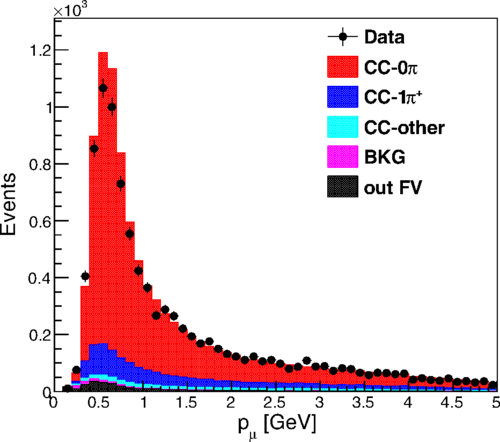
\includegraphics[height=0.25\textheight]{Chapters/Figures/SamplesAndSelections/cc0pi_selection}
\par\end{centering}
}\subfloat[$\protect\numubar$ CC-0$\pi$ Selection\cite{Campbell2018a}]{\begin{centering}
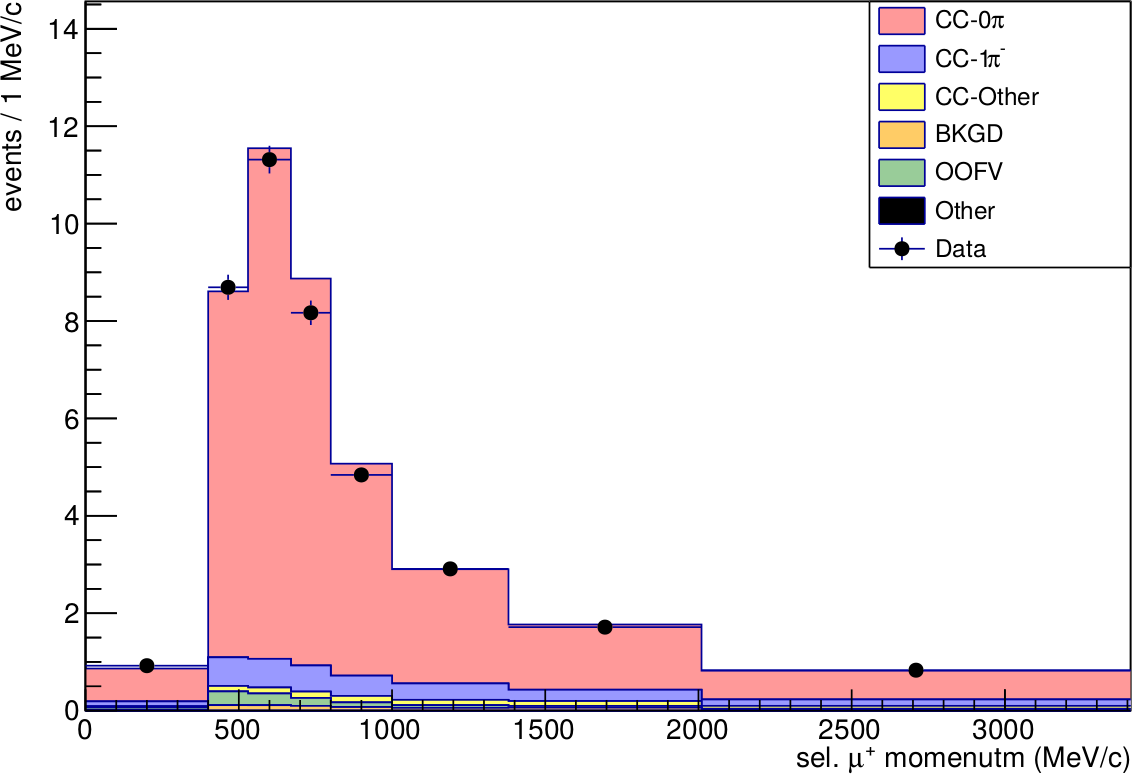
\includegraphics[height=0.25\textheight]{Chapters/Figures/SamplesAndSelections/numubarcc0pi_selection}
\par\end{centering}
}
\par\end{centering}
\caption[The \podtitle{} \numutitle{} and \numubartitle{} CC-$0\pi$ Selection
Kinematics]{The $\pod$ $\protect\numu$ and $\protect\numubar$ CC-$0\pi$ selection
kinematics. They importantly share the same pre-selection cuts as
this analysis. The error bars are statistical only with the prediction
sorted into various truth topologies.\label{fig:numuandnumubarCC0pi}}
\end{figure}

This paragraph is a layout of the topics in the chapter. First discussed
is the event reconstruction using the ``Global'' reconstruction
software in \prettyref{sec:The-ND280-Global-Reco}. The next discussion
is on the sample selections in \prettyref{sec:The-P0D-Selection-Cuts}.
With the selections established, three CC-inclusive selection are
described in the following order: the $\numu$ in foreword horn current
(FHC) mode selection, the $\numubar$ in reverse horn current (RHC)
mode selection, and the $\numu$ background in RHC mode selection.
The penultimate topic is an examination of the collected samples and
their kinematic properties in \prettyref{sec:Selection-Kinematics}.
Finally, the chapter summary is provided in \prettyref{sec:SelectionSummary}.


\section{The ND280 Global Reconstruction\label{sec:The-ND280-Global-Reco}}

The task of the Global reconstruction is to combine all of the ND280
information into a combined reconstructed object. It was originally
designed to identify CC-$0\pi$ events in the Tracker, FGD+TPC, region
and has been extended to operate with all of ND280.

The Global reconstruction is a software package that attempts to recognize
patterns of deposited energy in ND280 and categorize it accordingly.
Particles that deposit energy in long, linear segments are categorized
as tracks. If multiple tracks originate from a common origin (vertex),
it is likely that a true neutrino interaction event occurred near
the reconstructed vertex. Particle cascade or shower reconstruction
in Global will not be discussed since they are not selected in this
technote.

Each subdetector reconstruction algorithm is run separately as the
seed to Global's track matching algorithms. This includes the $\pod$'s
track-finding algorithm, which defines a $\pod$ track as a linear
sequence of ``nodes'' with one node at each bar layer. Each node
represents the approximate position where the particle intersected
the bar layer. To facilitate inter-detector matching, Global attempts
to ``re-fit'' the $\pod$ track using a Kalman filter\cite{kalmanFilter}.
The re-fit procedure also corrects for particle energy loss as a function
of length and multiple scattering processes. A $\pod$ vertex, which
is the assumed location of the neutrino interaction, is then associated
with the re-fit track using another Kalman filter algorithm. Matching
tracks between the $\pod$ and the TPC is done automatically in the
ND280 Global fit.


\section[Selection Cuts]{The \podtitle{} Selection Cuts\label{sec:The-P0D-Selection-Cuts}}

The selection of CC-inclusive events uses a series of cuts to select
the muon track. Prior to any cuts and after the reconstruction, corrections
are applied first to both data and MC events to correct for well known
residual differences between them. This includes correcting the MC
flux prediction using the secondary beamline data and reconstruction
efficiency corrections. A complete list of the corrections applied
are given in the following reference\cite{Abe2015c}. The pre-selection
cuts (``precuts'') are then applied to extract events that start
in the $\pod$ water target (WT) fiducial volume (FV).

The following sections will describe the precuts common to all CC-inclusive
selections. The next section describes the specific selections and
their cuts to select the main track associated as the lepton candidate.
Finally the lepton candidate and event kinematics for all the samples
are described.

\subsection{Precuts\label{subsec:Precuts}}

The precuts were initially developed to select $\numu$ CC-inclusive
events using the $\pod$ and TPC subdetector reconstruction algorithms
separately\cite{AbePhyRevD9652017,Das2016}. They were then used with
the Global reconstruction software for the $\numu$ $\cczeropi$ selection
in the FHC beam configuration\cite{PhysRevD.97.012001}. All cuts
were implemented in psyche\cite{Soto2017} which is the software interface
that BANFF uses to select events.

Prior to the precuts, neutrino interaction data event must be collected
and reconstructed for each T2K beam spill. Each T2K beam spill has
eight bunches that are 58 ns long and temporally separated by 581
ns. When the beam spill occurs, the $\pod$'s Trip-T electronics are
triggered to collect data in preset integration cycles aligned with
the bunches. Each integration cycle is 480 ns long and is followed
by a 100 ns dead-time to prepare for the next cycle\cite{Das2016}.
The data collected in each cycle is used to reconstruct neutrino interaction
events using the ND280 subdetector and Global software packages.

Each reconstructed event must pass the following cuts before being
assigned to a selection:
\begin{enumerate}
\item The event has a ``good'' data quality flag.
\begin{itemize}
\item An event is rejected if any electronics element or subdetector in
ND280 is reported as ``bad'' during the corresponding bunch.
\end{itemize}
\item There is at least one (1) track reconstructed in the TPC.
\begin{itemize}
\item There are no restrictions on the number of tracks fully contained
in the $\pod$ or exiting into other subdetectors. 
\end{itemize}
\item The track in the TPC must have more than 18 nodes.
\begin{itemize}
\item The TPC reconstruction gathers the vertical and horizontal micromegas
that registered collected charge into clusters of ``hits''. Each
cluster's charge distribution is used to get a vertical (horizontal)
position that is more accurate than the individual readout micromegas.
A node is constructed out of each cluster with associated track state
information. The set of nodes are used to fit a helix shaped track.
\end{itemize}
\item The reconstructed vertex is within the $\pod$ WT FV.
\begin{itemize}
\item The $\pod$ FV is defined to include as much of the WT regions as
possible. Its X and Y borders are 25 cm away from the $\pod$ule edges
while the Z borders intersect the last and first half downstream $\pod$ule
in the upstream ECal and central ECal, respectively. The FV edges
are listed in \prettyref{tab:FVDef}. This volume, while used for
track-based analyzes in the past, was optimized for $\pizero$ and
$\nue$ analyses.
\end{itemize}
\item All tracks that enter the TPC pass the veto cut
\begin{itemize}
\item An event is rejected if any $\pod$ track enters the TPC from outside
the ``corridor'' volume. This cut was designed to eliminate broken
tracks when the pre-Global separate subdetector reconstruction was
used \cite{Campbell2014}. In practice, this cut ensures that Global
tracks entering the TPC are away from its X and Y edges. The corridor
definition is the same as defined in the $\numubar/\numu$ cross section
ratio analysis technical note\cite{Campbell2017} and shown in \prettyref{tab:FVDef}.
\end{itemize}
\end{enumerate}
\begin{table}[H]
\caption[The \podtitle{} Water Target Fiducial Volume and Veto Corridor Definitions]{The $\pod$ WT FV (left) and veto corridor volume (right) in the
ND280 coordinate system. The corridor spans from the 5th (8th) to
40th (80th) $\pod$ule (scintillator layer). All the units are given
in millimeters.\label{tab:FVDef}}

\centering{}%
\begin{tabular}{cc}
\toprule 
\multicolumn{1}{c}{$\pod$ WT FV} & \multicolumn{1}{c}{Corridor Volume}\tabularnewline
\midrule
\midrule 
$-836<X<764$ & $-988<X<910$\tabularnewline
$-871<Y<869$ & $-1020<Y<1010$\tabularnewline
$-2969<Z<-1264$ & $-3139<Z<-900$\tabularnewline
\bottomrule
\end{tabular}
\end{table}

After passing of all the precuts, a single, global track, which is
observed in the TPC, is assigned as the lepton candidate or ``main
track'' of a selected event. While the main track is different for
each selected event, the momentum reconstruction is the same. The
momentum of the main track, $P$, is sum of its measured momentum
in the TPC, $P_{\text{TPC}}$, with the estimate momentum lost in
the $\pod$, $\Delta P_{\pod}$
\begin{equation}
P=P_{\text{TPC}}+\Delta P_{\pod}.\label{eq:momentumP0D}
\end{equation}
The momentum lost in the $\pod$ is estimated by summing the total
momentum loss along the track path $\mathcal{C}$ 
\begin{equation}
\Delta P=\int_{\mathcal{C}}\left(\frac{dP}{dx}\right)dx,\label{eq:energyloss}
\end{equation}
where $dP/dx$ is the momentum loss function. The momentum loss function
is related to the energy loss function, $dE/dx$ via the chain rule
\begin{equation}
\begin{aligned}\frac{dE}{dx} & =\left(\frac{dE}{dP}\right)\left(\frac{dP}{dx}\right)\\
 & =\frac{d}{dP}\left(\sqrt{P^{2}c^{2}+m^{2}c^{4}}\right)\left(\frac{dP}{dx}\right)\\
 & =\left(\frac{Pc^{2}}{E}\right)\left(\frac{dP}{dx}\right)\\
 & =\beta c\left(\frac{dP}{dx}\right),
\end{aligned}
\label{eq:chainrule}
\end{equation}
where $\beta$ is the particle velocity as a ratio of the speed of
light $c$. Since the reconstructed track's path $\mathcal{C}$ is
not infinitesimally precise due to inherent detector resolution, we
must replace the integral with a sum and differential $dx\rightarrow\Delta x$.
We then arrive at the expression of the momentum loss estimate in
the $\pod$ as
\begin{equation}
\Delta P_{\pod}=\frac{1}{c}\sum_{t}\left[\left(\frac{dE}{dx}\right)\left(\frac{\Delta x}{\beta}\right)\right]_{t},\label{eq:momentumP0DFull}
\end{equation}
where $t$ is a discrete step in $x$ connecting the track nodes.
For most tracks entering the TPC, they will be highly relativistic
in the $\pod$ ($\beta\approx1$), and \eqref{eq:momentumP0DFull}
simplifies to 
\begin{equation}
\Delta P_{\pod}=\frac{1}{c}\sum_{t}\left[\left(\frac{dE}{dx}\right)\Delta x\right]_{t}.\label{eq:momentumP0DSimplified}
\end{equation}
The next sections describe the selection cuts, first in FHC mode and
then RHC mode.

\subsection{The \numutitle{} in FHC Mode CC-Inclusive Selection \label{subsec:numuCCInclusive}}

As discussed in \mbox{Section~\ref{subsec:Precuts}}, this selection
is the basis for the $\pod$ $\numu$ $\cczeropi$ analysis\cite{PhysRevD.97.012001}.
In FHC mode, the vast majority of neutrino interactions are $\numu$
CC events that produce an outgoing, negatively charged muon. If there
is no negatively charged track in the TPC, the event is likely not
a $\numu$-induced interaction. Therefore, the $\numu$ in FHC mode
CC-inclusive selection in FHC mode has one final cut after the precuts:
\begin{enumerate}
\item At least one negatively charged track is reconstructed in the TPC.
\begin{itemize}
\item An event is rejected if none of the TPC tracks have a reported negative
curvature.
\end{itemize}
\end{enumerate}
If the event passes this cut, the highest momentum negative (curvature)
track, or HMNT, is selected as the lepton candidate. This selection
and all subsequent selections are branched into two categories based
on the number of tracks counted in the $\pod$. If there is only one
$\pod$ track, and hence only one track in the TPC as required by
the precuts, the event is categorized as a ``$\numu$ in FHC Mode
CC 1-Track'' event. Otherwise, the event is categorized as a ``$\numu$
in FHC Mode CC N-Tracks'' event.

\subsection{The \numubartitle{} in RHC Mode CC-Inclusive Selection \label{subsec:numubarRHCCCInclusive}}

In RHC mode, the majority of the beam neutrinos are $\numubar$ since
the horn focuses negatively charged pions and deflects positively
charged pions. However, the $\numu$ background interaction rate in
RHC mode is larger than the $\numubar$ background in FHC mode. The
reason for this is two fold. Firstly, the antineutrino-nuclear scattering
cross section is suppressed by \textasciitilde 1/3 compared to the
neutrino-nuclear scattering cross section as explained in \mbox{Section~\ref{subsec:Neutrino-Scattering-with-Matter}}.
Secondly, the $\numu$ flux in RHC is relatively large due to the
excess of positively charged pions generated at the target. Therefore
there is a non-negligible ``wrong-sign'' background in RHC mode
that we need to reject.

Prior to this analysis, a $\numubar$ CC-$0\pi$ selection was developed
for the $\pod$\cite{Campbell2018a}. The $\numubar$ CC-$0\pi$ selection
is quite similar to the $\numu$ CC-inclusive selection in FHC mode,
but relied on the $\pod$ local reconstruction for a particle identification
cut. The $\pod$ local reconstruction is, however, unavailable in
the event selection software used in the BANFF fit called psyche.
So a new selection was developed specifically for this analysis to
select $\numubar$ interactions in RHC mode.

The $\numubar$ in RHC mode CC-inclusive selection uses the precuts
described in \mbox{Section~\ref{subsec:Precuts}} and the has two
cuts:
\begin{enumerate}
\item At least one positively charged track is reconstructed in the TPC.
\begin{itemize}
\item An event is rejected if none of the TPC tracks have a reported positive
curvature.
\end{itemize}
\item The highest momentum positive (curvature) track, or HMPT, must be
the highest momentum track.
\begin{itemize}
\item If the highest momentum track has negative curvature, then the event
is rejected.
\end{itemize}
\end{enumerate}
If the event passes these two cuts, the HMPT is the lepton candidate.
If there is only one $\pod$ track, the event is categorized as a
``$\numubar$ in RHC Mode CC 1-Track'' event. Otherwise, the event
is categorized as a ``$\numubar$ in RHC Mode CC N-Tracks'' event.

\subsection{The \numutitle{} in RHC Mode CC-Inclusive Selection \label{subsec:numuRHCCCInclusive}}

As explained in the previous subsection, the $\numu$ background interaction
rate in RHC mode is relatively large compared to the $\numubar$ interaction
rate. Having a measurement of this background is critical for the
oscillation analysis due to the small number of expected $\numubar\rightarrow\nuebar$
counts. To date, there is no $\pod$ measurement of $\numu$ background
in RHC mode, nor any $\pod$ selection to do so. So like the $\numubar$
CC-inclusive selection, a new $\pod$ selection was developed exclusively
for this analysis to select $\numu$ background events in RHC mode.

The $\numu$ background in RHC mode CC-inclusive selection uses the
precuts described in Subsection \ref{subsec:Precuts} and has two
cuts:
\begin{enumerate}
\item At least one negatively charged track is reconstructed in the TPC.
\begin{itemize}
\item An event is rejected if none of the TPC tracks have a reported negative
curvature.
\end{itemize}
\item The HMNT must be the highest momentum track.
\begin{itemize}
\item If the highest momentum track has positive curvature, then the event
is rejected.
\end{itemize}
\end{enumerate}
If the event passes these two cuts, the HMNT is the lepton candidate.
If there is only one $\pod$ track, the event is categorized as a
``$\numu$ Background in RHC Mode CC 1-Track'' event. Otherwise,
the event is categorized as a ``$\numu$ Background in RHC Mode CC
N-Tracks'' event.


\section{Selection Kinematics\label{sec:Selection-Kinematics}}

This section examines the kinematics for each of selections and their
respective branches while differentiating between water-in and water-out
mode. The data sets used in this analysis are runs 2-8 in both $\pod$
water-in and water-out (air) modes as shown in \prettyref{tab:T2K-MC-Data-POT}.
There will be no data events shown to prevent any potential analysis
biases. Simulated events will be arranged into various true categories
to study selection kinematics, efficiencies, and purities.

\begin{table}
\caption[T2K Data-Taking Periods and Collected POT Used in the Analysis]{T2K data-taking periods and collected POT used in the analysis. The
bottom four rows are the aggregated periods grouped by horn current
and $\pod$ status, which is how the data analysis is performed. Note
that the horns were run briefly at +205 kA for Run 3b when operations
resumed after 2011 T\={o}hoku earthquake.\label{tab:T2K-MC-Data-POT}}

\centering{}%
\begin{tabular}{ccccc}
\toprule 
Run & Horn & $\pod$ & Data POT & MC POT\tabularnewline
period & current {[}kA{]} & status & $\left(\times10^{20}\right)$ & $\left(\times10^{20}\right)$\tabularnewline
\midrule
\midrule 
2 & +250 & Water & 0.433934 & 12.0341\tabularnewline
 &  & Air & 0.359149 & 9.23937\tabularnewline
3b & +205 &  & 0.217273 & 4.47864\tabularnewline
3c & +250 &  & 1.36447 & 26.3227\tabularnewline
4 &  &  & 1.78271 & 34.996\tabularnewline
 &  & Water & 1.64277 & 34.9712\tabularnewline
5c & -250 &  & 0.43468 & 22.7766\tabularnewline
6b &  & Air & 1.28838 & 14.174\tabularnewline
6c &  &  & 0.505895 & 5.27562\tabularnewline
6d &  &  & 0.775302 & 6.884\tabularnewline
6e &  &  & 0.847902 & 8.59439\tabularnewline
7b &  & Water & 2.43682 & 33.7046\tabularnewline
8 & +250 &  & 1.58053 & 26.4664\tabularnewline
 &  & Air & 4.14897 & 36.0694\tabularnewline
Sand & +250 &  & - & 11.1988\tabularnewline
Sand & -250 &  & - & 12.9201\tabularnewline
\midrule
\midrule 
2, 3b, 3c, 4, 8 & FHC & Air & 7.872757 & 111.09\tabularnewline
2, 4, 8 &  & Water & 3.656589 & 73.47\tabularnewline
6b, 6c, 6d, 6e & RHC & Air & 3.382490 & 35.262\tabularnewline
5c, 7b &  & Water & 2.852340 & 54.53\tabularnewline
\bottomrule
\end{tabular}
\end{table}

True interactions for these selections are generally divided into
four classes:
\begin{itemize}
\item A neutrino-induced CCQE interaction ($\nu$ CCQE):
\begin{itemize}
\item Only NEUT generated neutrino-induced CCQE event at the interaction
vertex.
\end{itemize}
\item A neutrino-induced non-CCQE interaction ($\nu$ non-CCQE):
\begin{itemize}
\item Any NEUT generated neutrino-induced CC and NC event \textit{except}
neutrino-induced CCQE at the interaction vertex.
\end{itemize}
\item An antineutrino-induced CCQE interaction ($\overline{\nu}$ CCQE):
\begin{itemize}
\item Only NEUT generated antineutrino-induced CCQE event at the interaction
vertex.
\end{itemize}
\item An antineutrino-induced non-CCQE interaction ($\overline{\nu}$ non-CCQE):
\begin{itemize}
\item Any NEUT generated antineutrino-induced CC and NC event \textit{except}
antineutrino-induced CCQE at the interaction vertex.
\end{itemize}
\end{itemize}
These signal classes must occur in the $\pod$ WT FV in order to be
selected. The non-CCQE category can be further divided among the dominant
T2K CC and all NC interactions modes as enumerated in \prettyref{tab:NEUTReaction}.
An out of FV (OOFV) event is any true event that occurs in ND280,
but is falsely reconstructed in the $\pod$ FV. Another important
ND280 background are true neutrino and antineutrino CC interactions
occurring in the sand surrounding the ND280 pit with the muon track
falsely reconstructed in the FV. These events are referred to as ``sand
muon'' events and are accounted for accordingly. Since these categories
are used frequently in this chapter, the legends used in the histograms
are enlarged for the reader's convenience in \prettyref{fig:enlarged_legends}.

\begin{table}
\caption[Enumeration of NEUT Interaction Modes]{Enumeration of the NEUT interaction modes which are also used in
\prettyref{fig:enlarged_legends}. An arrow indicates a sequence of
integer steps from left to right of the arrow. \label{tab:NEUTReaction}}

\centering{}%
\begin{tabular}{clc}
\toprule 
\multicolumn{2}{c}{Interaction mode} & $\nu$ ($\antinu$) NEUT enumeration\tabularnewline
\midrule
\midrule 
\multicolumn{2}{c}{CCQE} & $1$ ($-1$)\tabularnewline
\midrule 
 & 2p2h & $2$ ($-2)$\tabularnewline
\cmidrule{2-3} \cmidrule{3-3} 
 & CC-$1\pi$ & $11\rightarrow16$ ($-11\rightarrow-16$)\tabularnewline
\cmidrule{2-3} \cmidrule{3-3} 
\multirow{2}{*}{non-CCQE} & CC-N$\pi$ & $21$ ($-21$)\tabularnewline
\cmidrule{2-3} \cmidrule{3-3} 
 & CC-DIS & $26$ ($-26$)\tabularnewline
\cmidrule{2-3} \cmidrule{3-3} 
 & CC-Other & $17,22,23$ ($-17,-22,-23$)\tabularnewline
\cmidrule{2-3} \cmidrule{3-3} 
 & NC & $31\rightarrow100$ ($-31\rightarrow-100$)\tabularnewline
\bottomrule
\end{tabular}
\end{table}

The ND280 MC uses the GEANT4 software toolkit \cite{Agostinelli:2002hh}
to simulate the passage of particles through matter. A GEANT4 particle
is assigned to a reconstructed track if it contributed the most to
the track's reconstructed hits. The most likely truth matched particles
include protons (p), both negatively and positively charged muons
($\mu^{\pm}$), pions ($\pi^{\pm})$, and electrons/positrons ($e^{\pm})$.
In addition, any electron and positron generated from pair production
are grouped together as ``$e^{\pm}/\gamma$''. Particles that do
not match any of these categories is labeled as ``other''.

\begin{figure}
\begin{centering}
\subfloat[CCQE and non-CCQE]{\begin{centering}
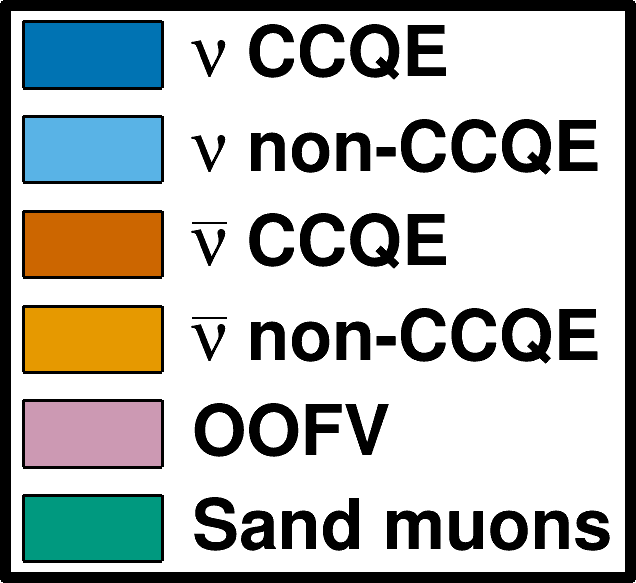
\includegraphics[height=1.32in]{Chapters/Figures/SamplesAndSelections/NEUTCCQELike_legend}
\par\end{centering}
}\subfloat[Neutrino interactions]{\begin{centering}
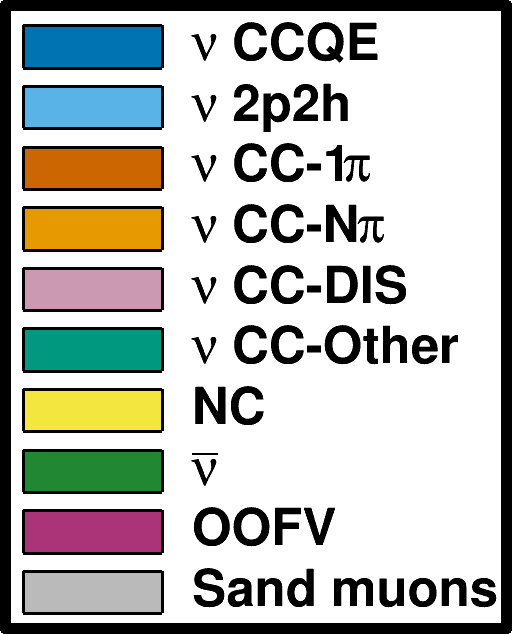
\includegraphics[height=2.26in]{Chapters/Figures/SamplesAndSelections/NEUTNuInteraction_legend}
\par\end{centering}
}\subfloat[Antineutrino interactions]{\centering{}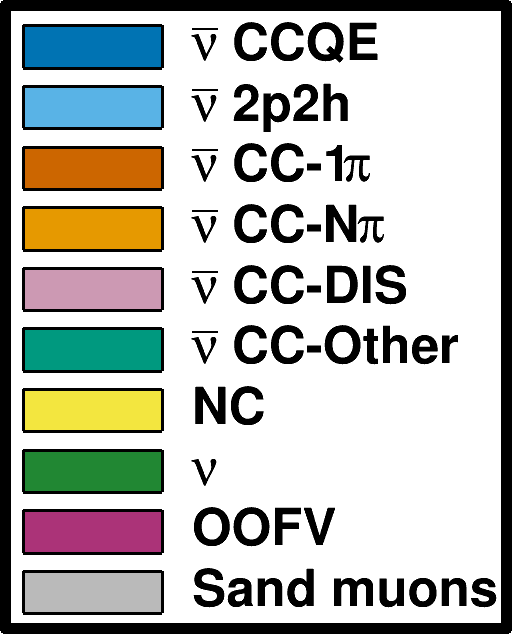
\includegraphics[height=2.26in]{Chapters/Figures/SamplesAndSelections/NEUTAntiNuInteraction_legend}}\subfloat[True particle]{\begin{centering}
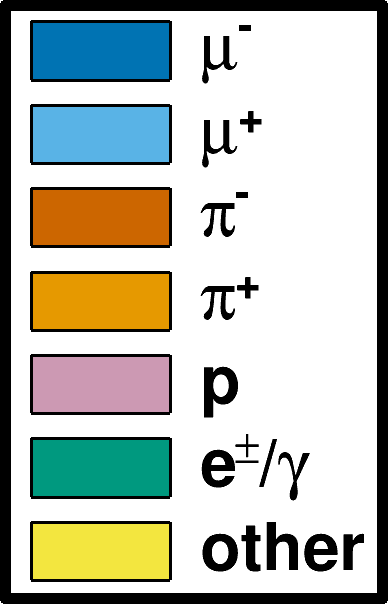
\includegraphics[height=1.57in]{Chapters/Figures/SamplesAndSelections/TrueParticle_legend}
\par\end{centering}
}
\par\end{centering}
\caption[Frequently Used Legends in the Analysis]{Frequently used legends that are enlarged for the reader's convenience.
\label{fig:enlarged_legends}}
\end{figure}


\subsection{The \numutitle{} in FHC Mode CC 1-Track Sample\label{subsec:numuFHCCC1Trk}}

This selection provides the CCQE-like samples in FHC mode. \prettyref{fig:numuFHCCC1TrkRecoCCQE}
and \prettyref{fig:numuFHCCC1TrkRecoParticle} displays the momentum
and angular distributions that are inputs to BANFF. Comparing between
water-in and water-out modes, we see that the reconstructed kinematics
are nearly identical. In the majority of cases, the lepton candidate
is the true muon, making this a very pure $\numu$ sample. We also
see that there are non-CCQE events, which without a particle identification
cut, are a irreducible background. Following this paragraph and the
following sections, only the $\pod$ water-in mode kinematics will
be shown.

\begin{figure}
\begin{centering}
\subfloat[Water-out Momentum]{\begin{centering}
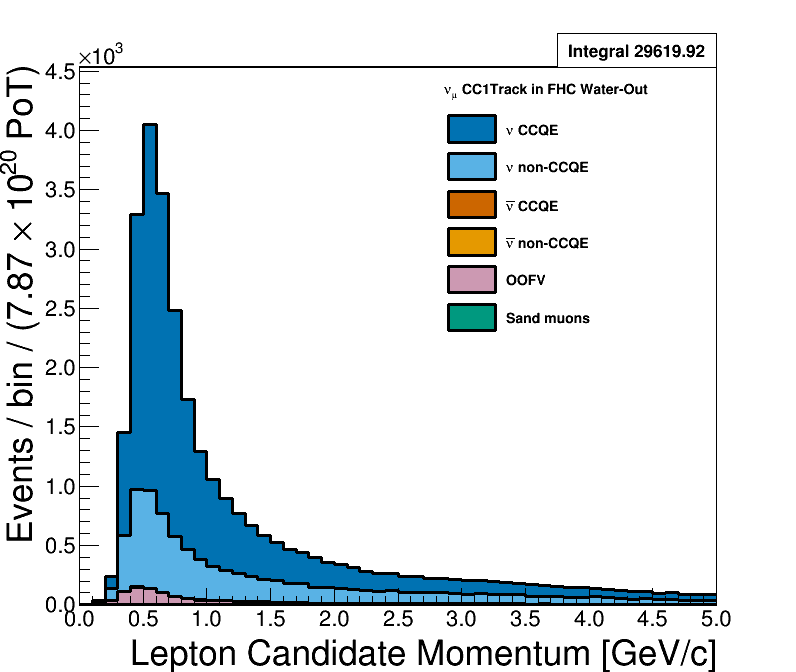
\includegraphics[width=0.45\textwidth]{Chapters/Figures/SamplesAndSelections/air/numu/CC1Track/FluxAndEventWeights/numuCC1TrackWaterOut_recoP_mu_MC_only_NEUTCCQELike_fhc_air}
\par\end{centering}
}\subfloat[Water-out $\cos\theta$]{\begin{centering}
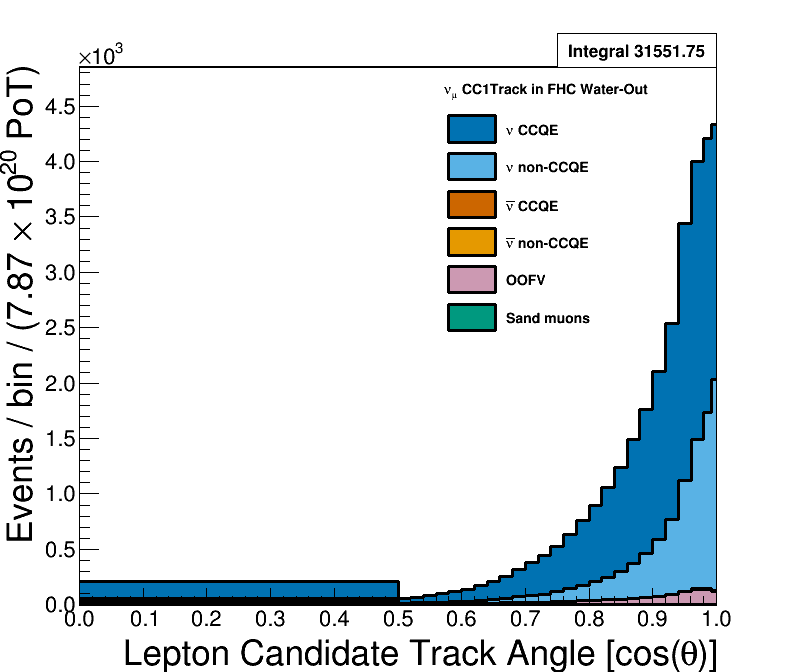
\includegraphics[width=0.45\textwidth]{Chapters/Figures/SamplesAndSelections/air/numu/CC1Track/FluxAndEventWeights/numuCC1TrackWaterOut_recocosq_mu_MC_only_NEUTCCQELike_fhc_air}
\par\end{centering}
}
\par\end{centering}
\begin{centering}
\subfloat[Water-in Momentum]{\begin{centering}
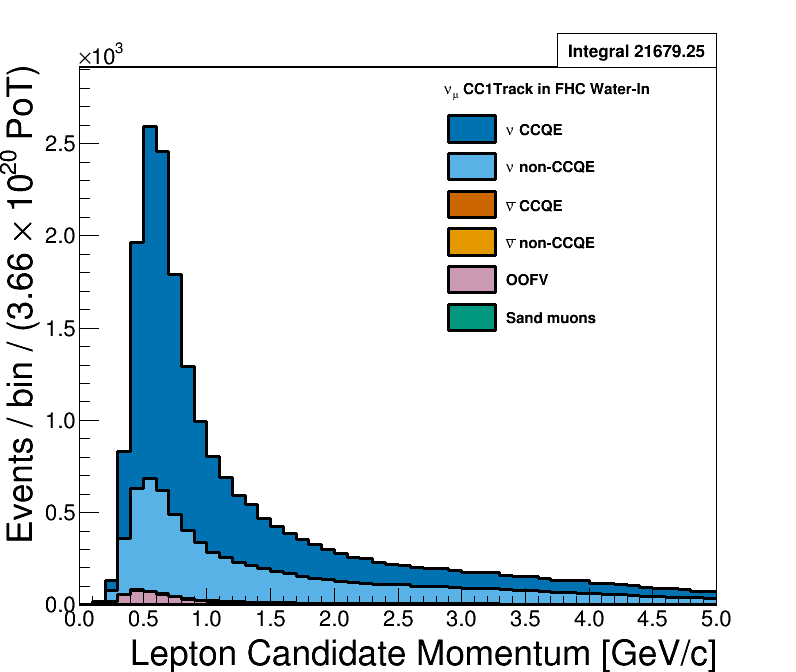
\includegraphics[width=0.45\textwidth]{Chapters/Figures/SamplesAndSelections/water/numu/CC1Track/FluxAndEventWeights/numuCC1TrackWaterIn_recoP_mu_MC_only_NEUTCCQELike_fhc_water}
\par\end{centering}
}\subfloat[Water-in $\cos\theta$]{\begin{centering}
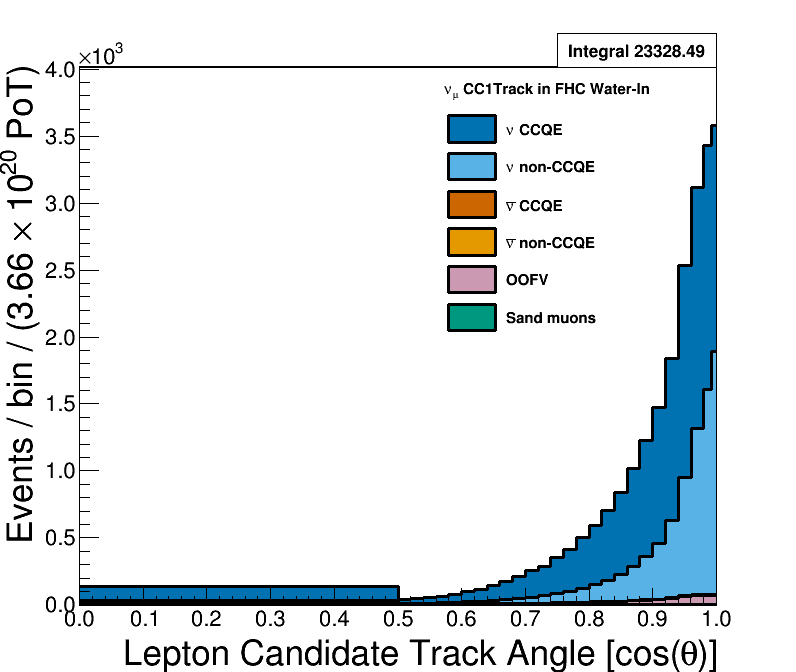
\includegraphics[width=0.45\textwidth]{Chapters/Figures/SamplesAndSelections/water/numu/CC1Track/FluxAndEventWeights/numuCC1TrackWaterIn_recocosq_mu_MC_only_NEUTCCQELike_fhc_water}
\par\end{centering}
}
\par\end{centering}
\caption[Reconstructed Kinematics of the $\numu$ in FHC Mode CC 1-Track Selection
Categorized by CCQE and Non-CCQE Interactions]{Reconstructed kinematics of the $\protect\numu$ in FHC Mode CC 1-Track
selection categorized by CCQE and non-CCQE interactions. The top figures,
(a) and (b), use the $\pod$ water-out MC and are normalized to the
FHC water-out mode POT. The bottom figures, (c) and (d), use the $\pod$
water-in MC and are normalized to the FHC water-in mode POT. Also
a single bin is used in the range of $0\protect\leq\cos\theta<0.5$
in figures (b) and (d).\label{fig:numuFHCCC1TrkRecoCCQE}}
\end{figure}

\begin{figure}
\begin{centering}
\subfloat[Water-out Momentum]{\begin{centering}
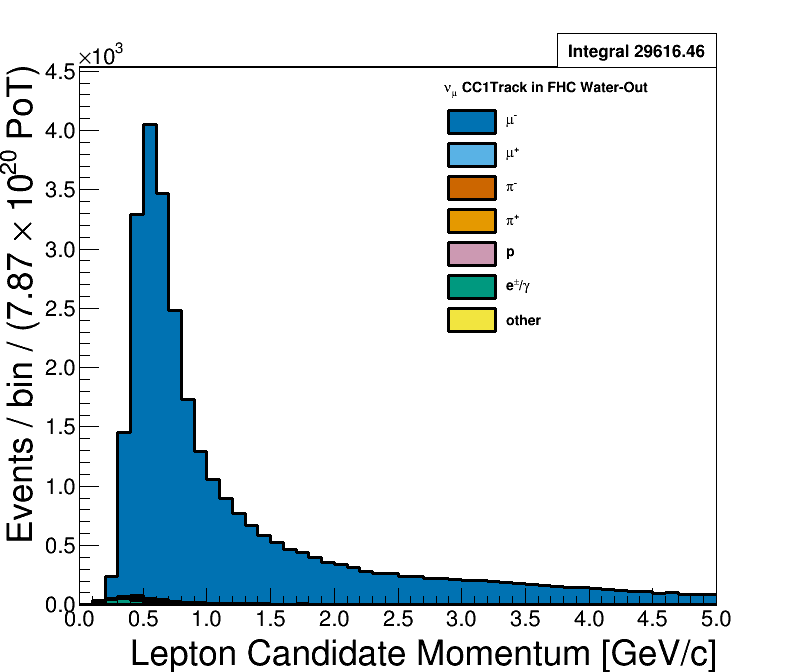
\includegraphics[width=0.45\textwidth]{Chapters/Figures/SamplesAndSelections/air/numu/CC1Track/FluxAndEventWeights/numuCC1TrackWaterOut_recoP_mu_MC_only_LeptonCandidateTruePDG_fhc_air}
\par\end{centering}
}\subfloat[Water-out $\cos\theta$]{\begin{centering}
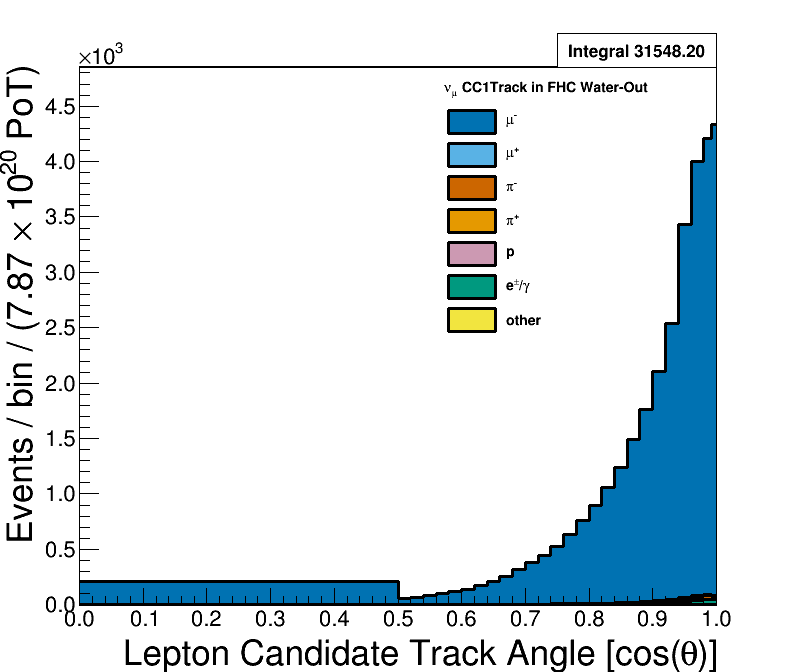
\includegraphics[width=0.45\textwidth]{Chapters/Figures/SamplesAndSelections/air/numu/CC1Track/FluxAndEventWeights/numuCC1TrackWaterOut_recocosq_mu_MC_only_LeptonCandidateTruePDG_fhc_air}
\par\end{centering}
}
\par\end{centering}
\begin{centering}
\subfloat[Water-in Momentum]{\begin{centering}
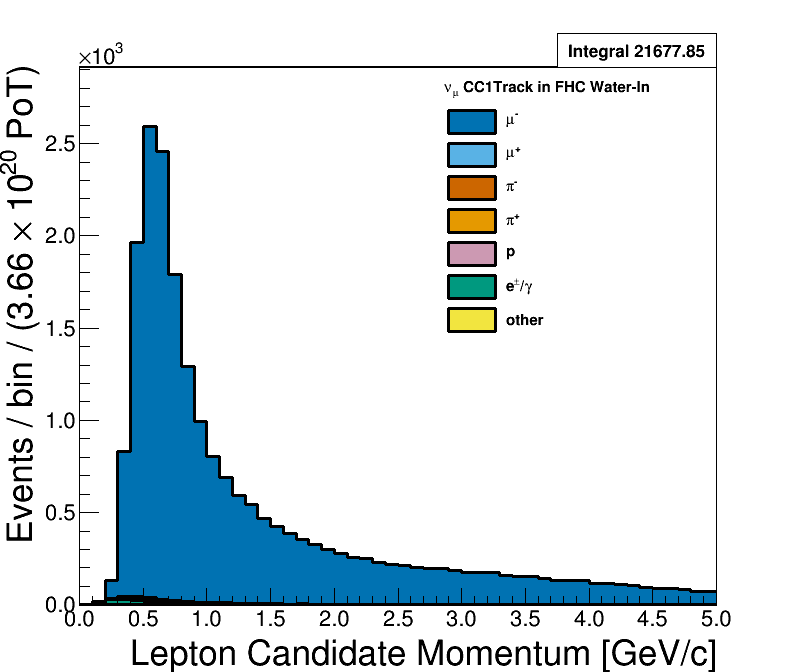
\includegraphics[width=0.45\textwidth]{Chapters/Figures/SamplesAndSelections/water/numu/CC1Track/FluxAndEventWeights/numuCC1TrackWaterIn_recoP_mu_MC_only_LeptonCandidateTruePDG_fhc_water}
\par\end{centering}
}\subfloat[Water-in $\cos\theta$]{\begin{centering}
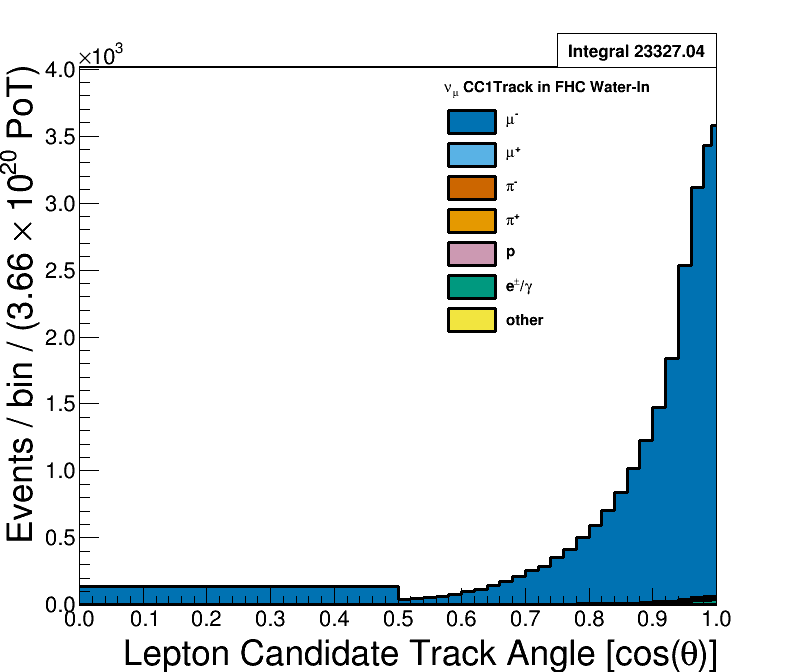
\includegraphics[width=0.45\textwidth]{Chapters/Figures/SamplesAndSelections/water/numu/CC1Track/FluxAndEventWeights/numuCC1TrackWaterIn_recocosq_mu_MC_only_LeptonCandidateTruePDG_fhc_water}
\par\end{centering}
}
\par\end{centering}
\caption[Reconstructed Kinematics of the $\numu$ in FHC Mode CC 1-Track Selection
Categorized by the True Particle Matched to the Main Track]{Reconstructed kinematics of the $\protect\numu$ in FHC Mode CC 1-Track
selection categorized by the true particle matched to the main track.
The top figures, (a) and (b), use the $\pod$ water-out MC and are
normalized to the FHC water-out mode POT. The bottom figures, (c)
and (d), use the $\pod$ water-in MC and are normalized to the FHC
water-in mode POT. Also a single bin is used in the range of $0\protect\leq\cos\theta<0.5$
in figures (b) and (d).\label{fig:numuFHCCC1TrkRecoParticle}}
\end{figure}

The target nuclei between water-in and water-out modes is shown in
\prettyref{fig:Vertex-position-numucc1trk}. Scattering on the carbon
nucleus is the dominant interaction in both modes since the scintillating
bars are constructed of polyethylene \ce{[(CH_2CH_2)_n]} plastic.
In water-in mode, the oxygen nucleus is a significant target with
hydrogen having a small contribution as well. The brass layers between
the $\pod$ules and the water bags introduce copper and zinc nuclei
scattering events too. The events on lead nuclei are true OOFV and
primarily occur in the last $\podule$.

\begin{figure}
\begin{centering}
\subfloat[Water-in]{\begin{centering}
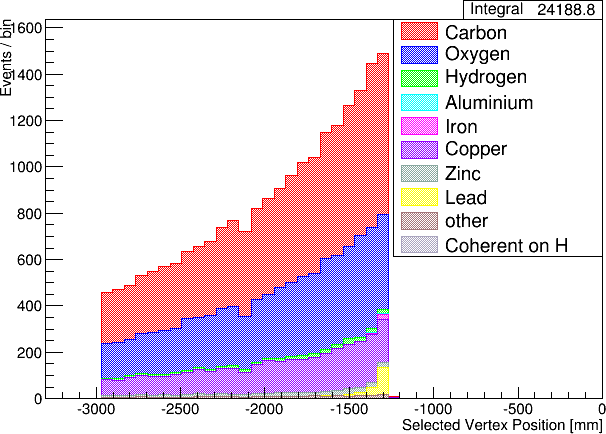
\includegraphics[width=0.45\textwidth]{Chapters/Figures/SamplesAndSelections/VertexZPosition_WaterIn_NumuFHCCC1Track}
\par\end{centering}
}\subfloat[Water-out]{\begin{centering}
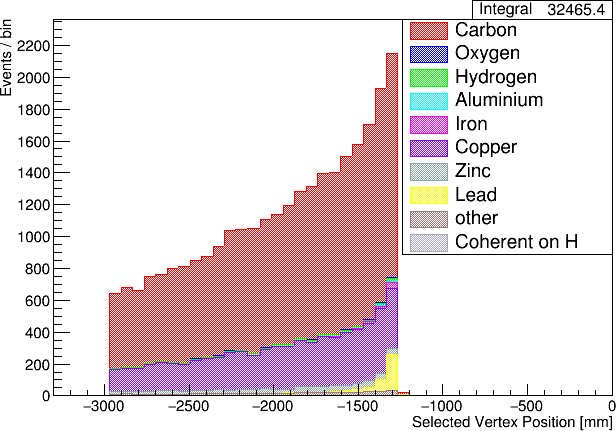
\includegraphics[width=0.45\textwidth]{Chapters/Figures/SamplesAndSelections/VertexZPosition_WaterOut_NumuFHCCC1Track}
\par\end{centering}
}
\par\end{centering}
\caption[Reconstructed Vertex Z Position of the $\numu$ in FHC Mode CC 1-Track
Selection]{Reconstructed vertex Z position of the $\protect\numu$ in FHC Mode
CC 1-Track selection. The events are categorized by the true target
nucleus. The number of selected events increases with increasing Z
since the probability of an interaction increases as the neutrino
crosses more media in the $\pod$. Due to a software bug in the MC,
coherent events on hydrogen (Coherent on H) are a unique category.\label{fig:Vertex-position-numucc1trk}}
\end{figure}

We can examine the efficiencies and purities differentially for true
$\numu$ CCQE interactions in \prettyref{fig:numuFHCCC1TrkRecoEffPur}.
The efficiency, $\epsilon$, and purity, $\rho$, are defined as
\begin{equation}
\epsilon=\frac{N_{\text{Selected}}^{\text{True}}}{N^{\text{True}}}\quad\rho=\frac{N_{\text{Selected}}^{\text{True}}}{N_{\text{Selected}}},\label{eq:effpur}
\end{equation}
where $N_{\text{Selected}}^{\text{True}}$ is the number of true,
selected events, $N^{\text{True}}$ is the number of true events,
and $N_{\text{Selected}}$ is the number of selected events. They
demonstrate that the purity is highest near $0.5$ GeV/c with the
efficiency highly dependent on the track angle.

\begin{figure}
\begin{centering}
\subfloat[True $\protect\numu$ CCQE Efficiency]{\begin{centering}
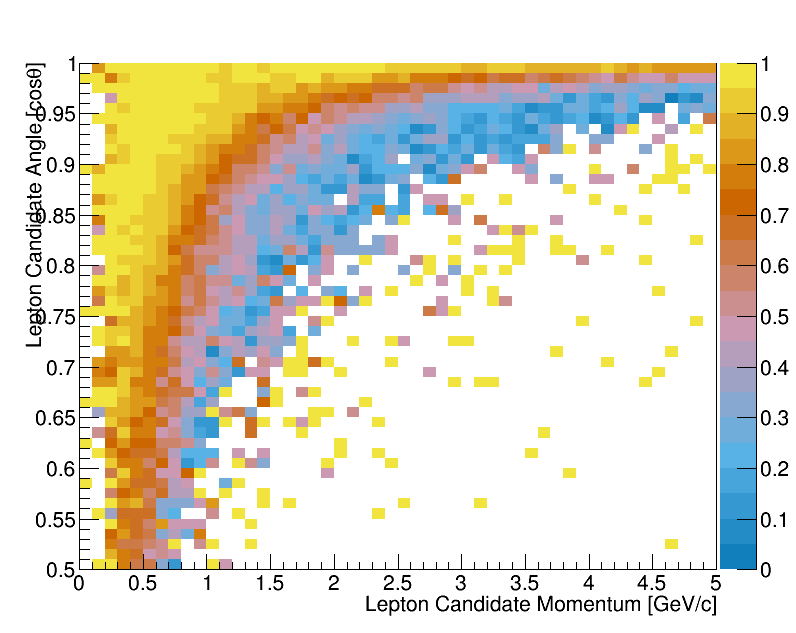
\includegraphics[width=0.45\textwidth]{Chapters/Figures/SamplesAndSelections/air/numu/CC1Track/FluxAndEventWeights/eff}
\par\end{centering}
}\subfloat[True $\protect\numu$ CCQE Purity]{\begin{centering}
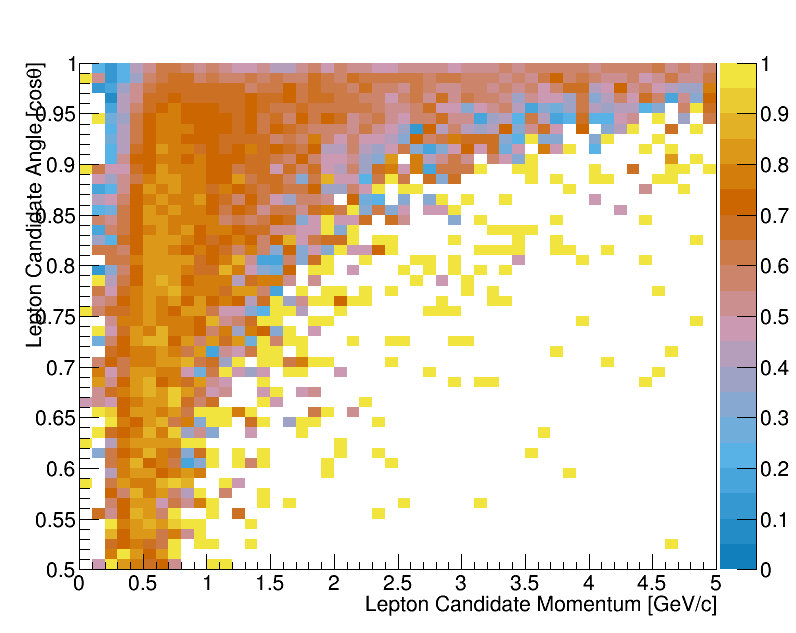
\includegraphics[width=0.45\textwidth]{Chapters/Figures/SamplesAndSelections/air/numu/CC1Track/FluxAndEventWeights/pur}
\par\end{centering}
}
\par\end{centering}
\caption[Efficiency and Purity of the $\numu$ in FHC Mode CC 1-Track Selection]{Efficiency and purity of the $\protect\numu$ in FHC Mode CC 1-Track
selection. True events are defined as correctly matched $\protect\muminus$
tracks from $\protect\numu$-induced CCQE interactions at the vertex.
\label{fig:numuFHCCC1TrkRecoEffPur}}
\end{figure}

The underlying true kinematics of the interactions are shown in \prettyref{fig:numuFHCCC1TrkTrue}.
Using \prettyref{fig:NuMuCCQE} as reference, the kinematics shown
are the true neutrino energy $E_{\nu}=k_{0}$ and 4-momentum transfer
$Q^{2}=-q^{2}$. These two variables are of theoretical importance
since they are used to generate events using NEUT and are used in
the BANFF fit. An interesting CCQE-like final state in this selection
are correlated nucleon pair scattering called ``2 particle, 2 hole''
(2p2h)\footnote{The name 2p2h originates from Condensed Matter Physics which motivated
the model. In solid state matter, a ``hole'' refers to the absence
of an electron in a valence band. In the High Energy Physics context,
2p2h considers neighboring and interacting nucleon pairs (2p) scattering
from an incoming neutrino. The imparted energy on the pair excites
them to higher energy states leaving two ``hole'' states (2h) behind.\medskip{}
} events\cite{Martini:2009uj}. Interaction model parameters for 2p2h
have large systematic uncertainties in T2K and are included the BANFF
fit. Therefore these events could help reduce the 2p2h model uncertainties.

\begin{figure}
\begin{centering}
\subfloat[True Neutrino Energy]{\begin{centering}
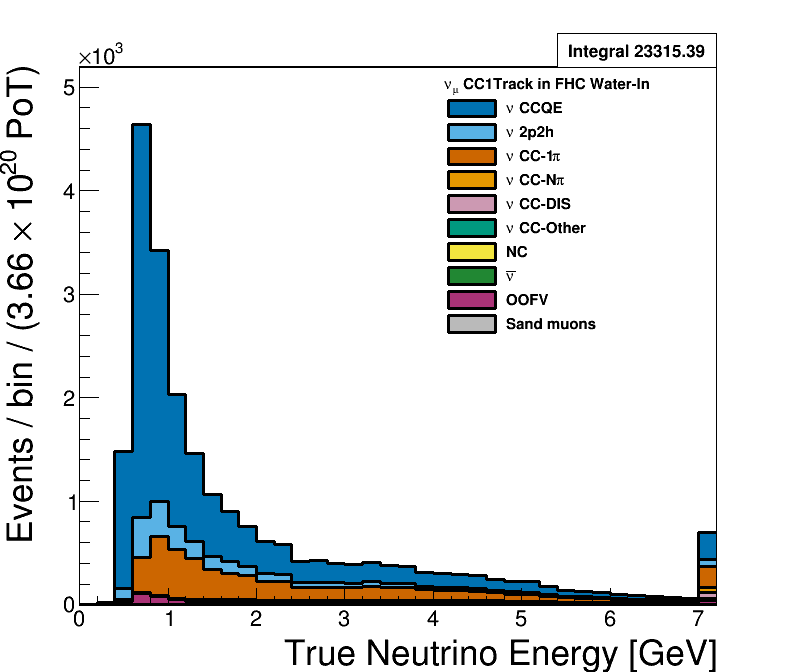
\includegraphics[width=0.45\textwidth]{Chapters/Figures/SamplesAndSelections/water/numu/CC1Track/FluxAndEventWeights/numuCC1TrackWaterIn_trueE_nu_MC_only_NEUTNuReactionCodes_fhc_water}
\par\end{centering}
}\subfloat[True $Q^{2}$]{\begin{centering}
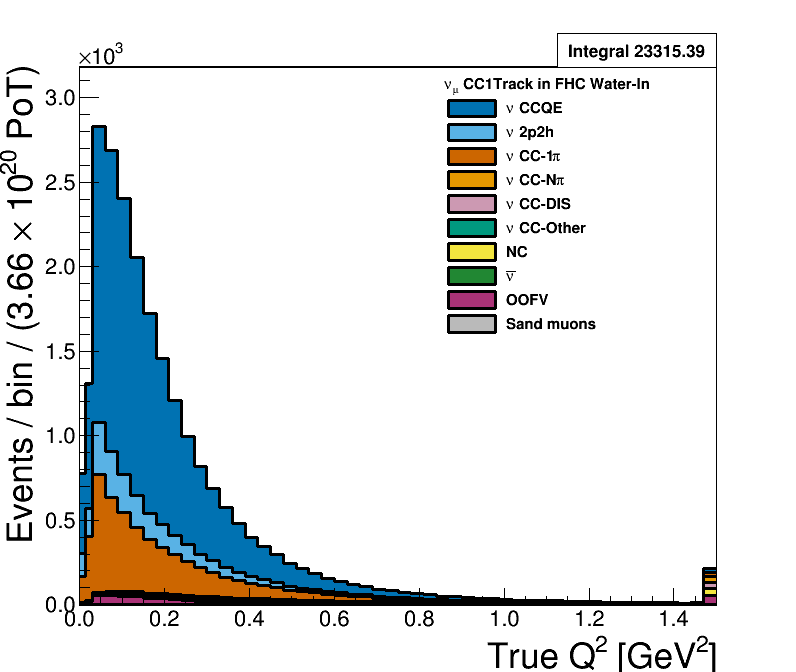
\includegraphics[width=0.45\textwidth]{Chapters/Figures/SamplesAndSelections/water/numu/CC1Track/FluxAndEventWeights/numuCC1TrackWaterIn_trueQ2_MC_only_NEUTNuReactionCodes_fhc_water}
\par\end{centering}
}
\par\end{centering}
\caption[True Kinematics of the $\numu$ in FHC Mode CC 1-Track Selection]{True kinematics of the $\protect\numu$ in FHC Mode CC 1-Track selection.
Water-in mode is displayed here only with the last bin shown is used
as overflow. The figures use the $\pod$ water-in MC and are normalized
to the FHC water-in mode POT. \label{fig:numuFHCCC1TrkTrue}}
\end{figure}

This selection contains a modest fraction of non-CCQE interactions.
The largest contamination is $1\pion$ interactions, which can happen
primarily for a couple of reasons. Firstly, when the final state pion
is produced, it is subject to final state interactions (FSI) where
a pion can be absorbed or scattered in the nucleus. Secondly, and
more importantly, a pion might not be reconstructed as a track in
the $\pod$ if its energy is below reconstruction threshold. Together,
the large $1\pion$ background affects the sensitivity to CC-$0\pi$
and CC-$1\pi$ model parameters in the BANFF fit.

\subsection{The \numutitle{} in FHC Mode CC N-Tracks Sample\label{subsec:numuFHCCCNTrk}}

This selection provides non-CCQE-like samples in FHC mode inputs to
the BANFF fit. The reconstructed momentum and angular distributions
are shown in \prettyref{fig:numuFHCCCNTrkRecoCCQE} and \prettyref{fig:numuFHCCCNTrkRecoParticle}.
Since this selection is not optimized for any particular CC topology,
there are a variety of interaction modes present including 1$\pion$,
multiple pion (N$\pion$) and deep inelastic scattering (DIS). There
are a number of events with a mis-identified main track that are matched
to electrons and pions. There is also a relatively larger OOFV contamination
compared with the 1-Track selection with some events originating in
the upstream ECal as seen in \prettyref{fig:Vertex-position-numuccNtrk}.
The vertex position and target materials are quite similar between
the 1-Track and N-Tracks selections.

\begin{figure}
\begin{centering}
\subfloat[Momentum]{\begin{centering}
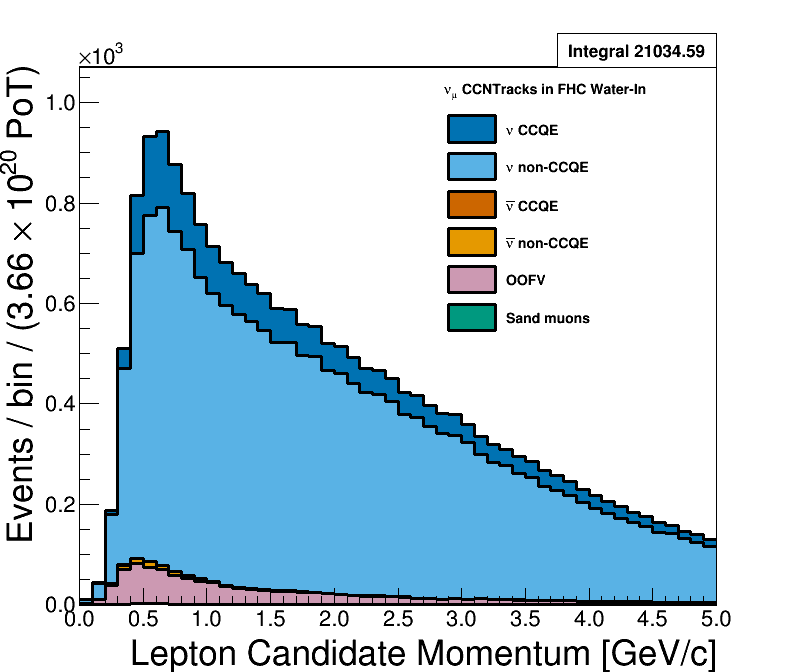
\includegraphics[width=0.45\textwidth]{Chapters/Figures/SamplesAndSelections/water/numu/CCNTracks/FluxAndEventWeights/numuCCNTracksWaterIn_recoP_mu_MC_only_NEUTCCQELike_fhc_water}
\par\end{centering}
}\subfloat[$\cos\theta$]{\begin{centering}
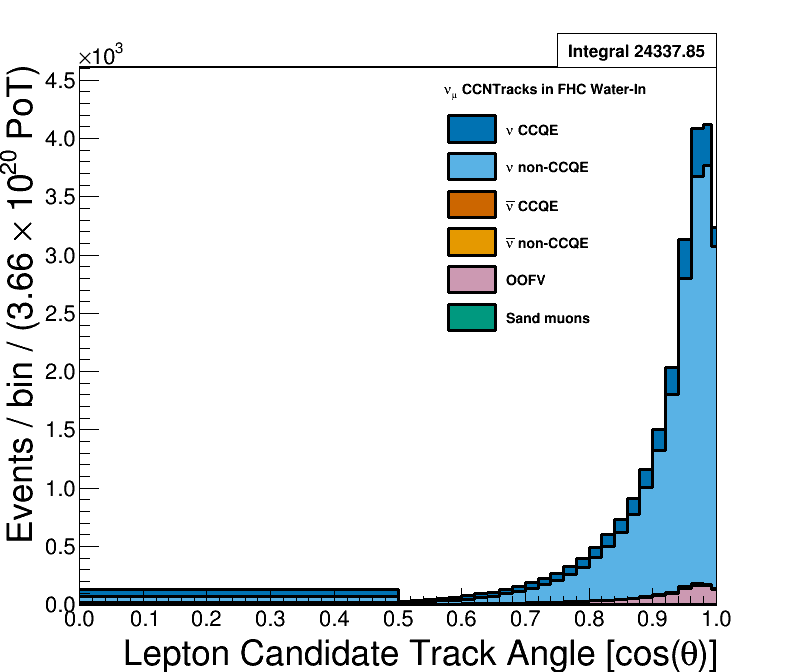
\includegraphics[width=0.45\textwidth]{Chapters/Figures/SamplesAndSelections/water/numu/CCNTracks/FluxAndEventWeights/numuCCNTracksWaterIn_recocosq_mu_MC_only_NEUTCCQELike_fhc_water}
\par\end{centering}
}
\par\end{centering}
\caption[Reconstructed Kinematics of the $\numu$ in FHC Mode CC N-Tracks Selection
Categorized by CCQE and Non-CCQE Interactions]{Reconstructed kinematics of the $\protect\numu$ in FHC Mode CC N-Tracks
selection categorized by CCQE and non-CCQE interactions. The figures
use the $\pod$ water-in MC and are normalized to the FHC water-in
mode POT. Also a single bin is used in the range of $0\protect\leq\cos\theta<0.5$
in figure (b).\label{fig:numuFHCCCNTrkRecoCCQE}}
\end{figure}

\begin{figure}
\begin{centering}
\subfloat[Momentum]{\begin{centering}
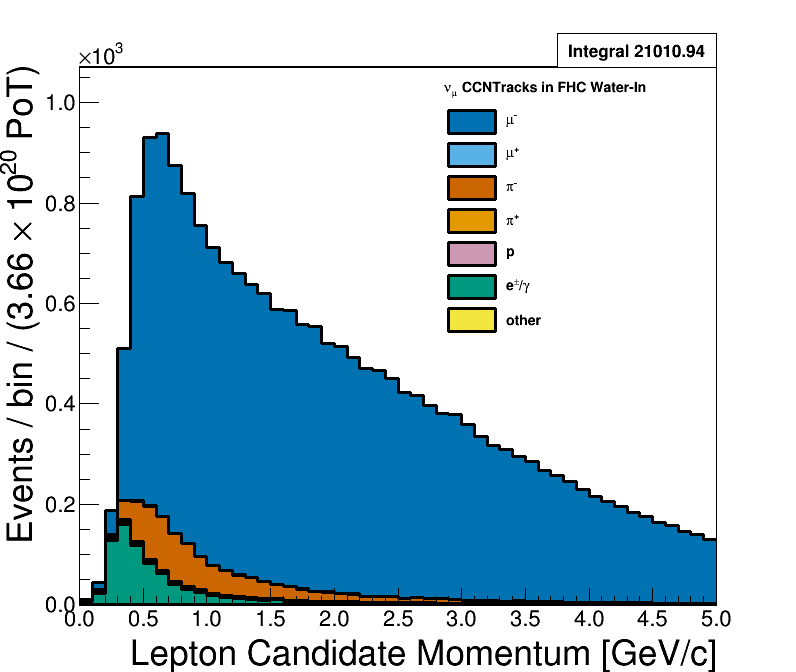
\includegraphics[width=0.45\textwidth]{Chapters/Figures/SamplesAndSelections/water/numu/CCNTracks/FluxAndEventWeights/numuCCNTracksWaterIn_recoP_mu_MC_only_LeptonCandidateTruePDG_fhc_water}
\par\end{centering}
}\subfloat[$\cos\theta$]{\begin{centering}
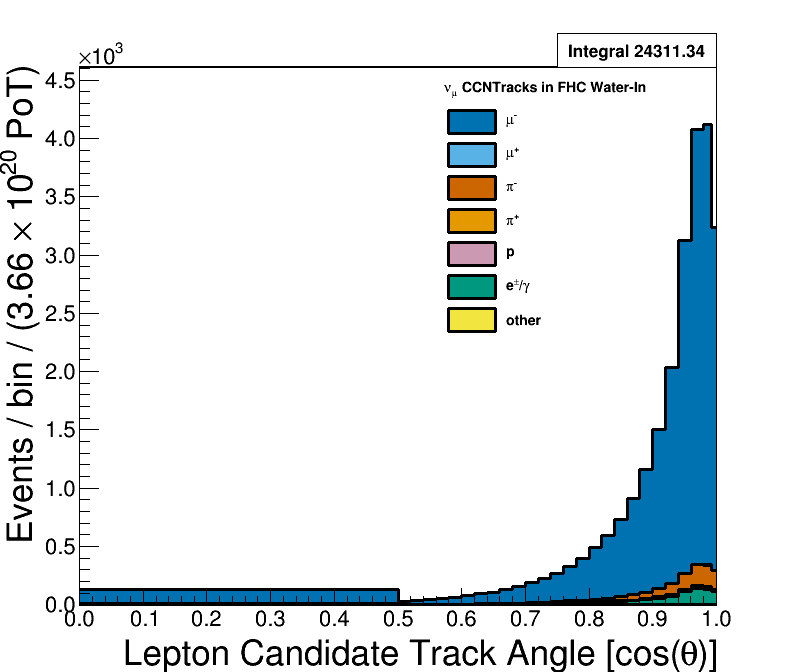
\includegraphics[width=0.45\textwidth]{Chapters/Figures/SamplesAndSelections/water/numu/CCNTracks/FluxAndEventWeights/numuCCNTracksWaterIn_recocosq_mu_MC_only_LeptonCandidateTruePDG_fhc_water}
\par\end{centering}
}
\par\end{centering}
\caption[Reconstructed Kinematics of the $\numu$ in FHC Mode CC N-Tracks Selection
Categorized by the True Particle Matched to the Main Track]{Reconstructed kinematics of the $\protect\numu$ in FHC Mode CC N-Tracks
selection categorized by the true particle matched to the main track.
The figures use the $\pod$ water-in MC and are normalized to the
FHC water-in mode POT. Also a single bin is used in the range of $0\protect\leq\cos\theta<0.5$
in figures (b) and (d).\label{fig:numuFHCCCNTrkRecoParticle}}
\end{figure}

\begin{figure}
\begin{centering}
\subfloat[Water-in]{\begin{centering}
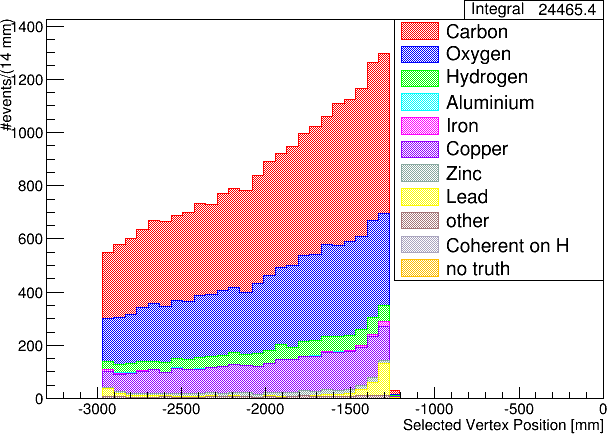
\includegraphics[width=0.45\textwidth]{Chapters/Figures/SamplesAndSelections/VertexZPosition_WaterIn_NumuFHCCCNTracks}
\par\end{centering}
}\subfloat[Water-out]{\begin{centering}
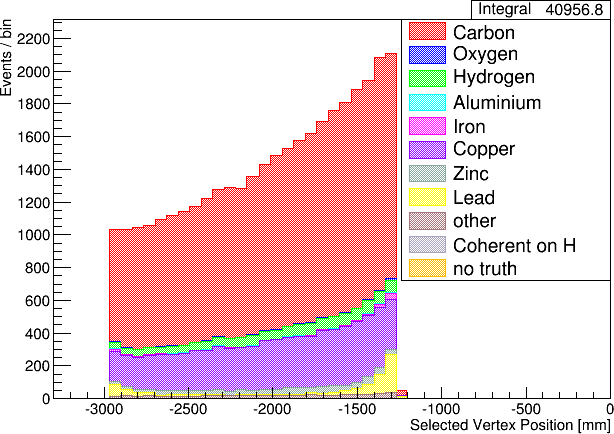
\includegraphics[width=0.45\textwidth]{Chapters/Figures/SamplesAndSelections/VertexZPosition_WaterOut_NumuFHCCCNTracks}
\par\end{centering}
}
\par\end{centering}
\caption[Reconstructed Vertex Z Position of the $\numu$ in FHC Mode CC N-Tracks
Selection Categorized by the True Target Nucleus]{Reconstructed vertex Z position of the $\protect\numu$ in FHC Mode
CC N-Tracks selection categorized by the true target nucleus. The
number of events increases with increasing Z since the probability
of an interaction increases as the neutrino crosses more media in
the $\pod$. Due to a software bug in the MC, coherent events on hydrogen
(Coherent on H) are a unique category.\label{fig:Vertex-position-numuccNtrk}}
\end{figure}

We can examine the efficiencies and purities differentially for the
selection in \prettyref{fig:numuFHCCCNTrkRecoEffPur}. For the efficiency
and purity only, the true signal is any $\numu$ CC interaction except
$\numu$ CCQE (CC non-QE), which the CC 1-Track topology selection
is designed to select. The efficiency is high for the higher momenta
and higher angle tracks suggesting this is a high $Q^{2}$ selection.
In addition, the purity is around \textasciitilde 70\% in this region.

\begin{figure}
\begin{centering}
\subfloat[True $\protect\numu$ CC non-QE Efficiency]{\begin{centering}
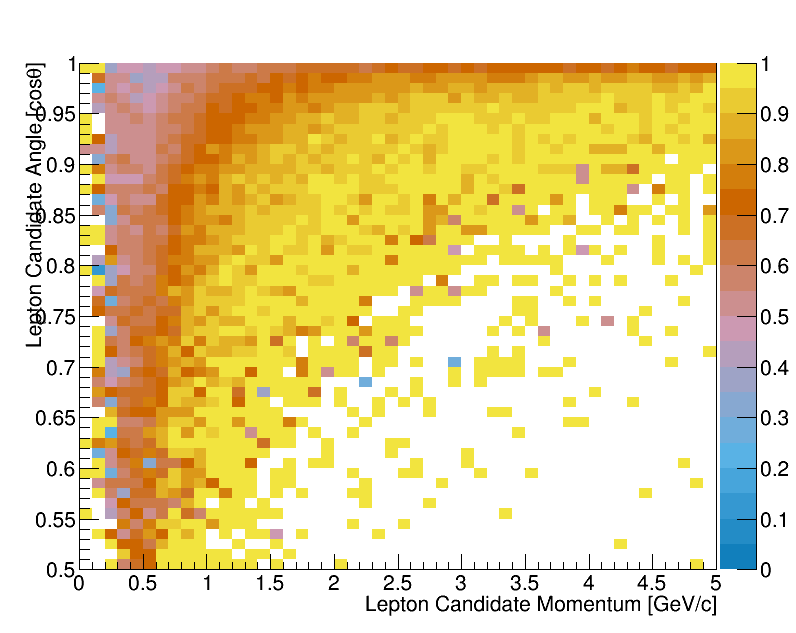
\includegraphics[width=0.45\textwidth]{Chapters/Figures/SamplesAndSelections/air/numu/CCNTracks/FluxAndEventWeights/eff}
\par\end{centering}
}\subfloat[True $\protect\numu$ CC non-QE Purity]{\begin{centering}
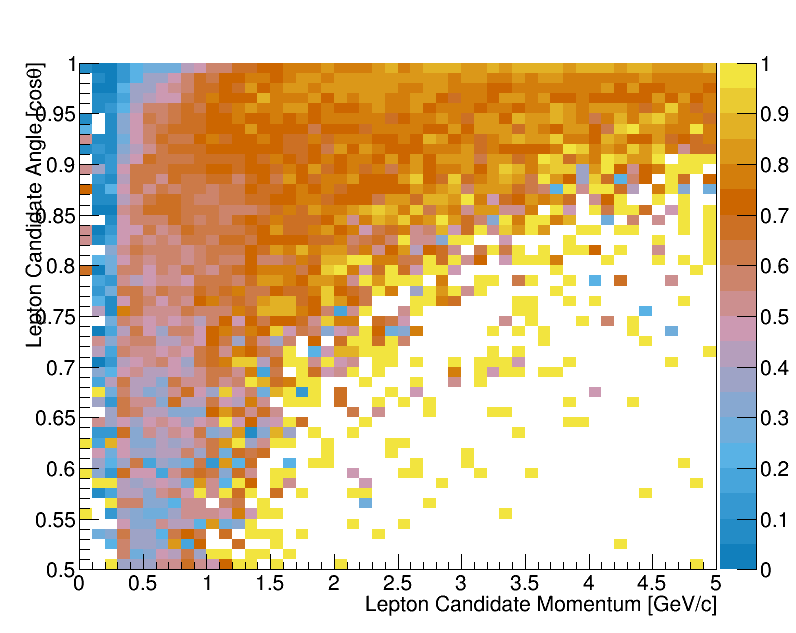
\includegraphics[width=0.45\textwidth]{Chapters/Figures/SamplesAndSelections/air/numu/CCNTracks/FluxAndEventWeights/pur}
\par\end{centering}
}
\par\end{centering}
\caption[Efficiency and Purity of the $\numu$ in FHC Mode CC N-Tracks Selection]{Efficiency and purity of the $\protect\numu$ in FHC Mode CC N-Tracks
selection. True events are defined as correctly matched $\protect\muminus$
tracks from $\protect\numu$-induced CC non-QE interactions at the
vertex.\label{fig:numuFHCCCNTrkRecoEffPur}}
\end{figure}

The fundamental kinematics of the selection are shown in \prettyref{fig:numuFHCCCNTrkTrue}.
The selection is relatively $\numu$-pure and captures the high energy
tail of the neutrino flux. True kinematics that describe the $1\pion,$
$N\pion$, and DIS models are parameterized in $Q^{2}$ and the hadronic
system mass $W$. Using \prettyref{fig:NuMuCCQE}, we can define the
invariant mass of hadronic system as
\begin{equation}
\begin{aligned}W^{2}c^{4} & =\left(p+q\right)^{2}=p^{2}+2p\cdot q+q^{2}\\
 & =M_{N}^{2}c^{4}+2M_{N}c^{2}\left(k_{0}-k_{0}^{\prime}\right)-Q^{2},
\end{aligned}
\label{eq:hadronicsystemmassW}
\end{equation}
where $M_{N}$ is the mass of the struck nucleon and $k_{0}$/$k_{0}^{\prime}$
is the energy of the neutrino/outgoing lepton. A dominant mode in
the selection is from the $1\pion$ interaction from a $\Delta$ resonance.
A resonance is clearly seen in the $W$ distribution in \prettyref{fig:numuFHCCCNTrkTrue},
which comes from the $\Delta$ baryon which has a rest mass of $1.232$
GeV/$\csq$.

\begin{figure}
\begin{centering}
\subfloat[True Neutrino Energy]{\begin{centering}
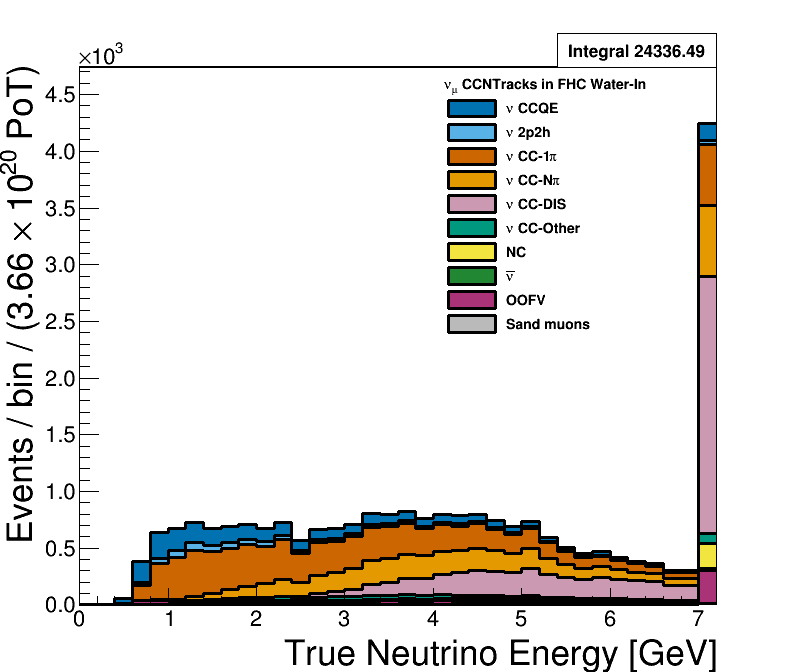
\includegraphics[width=0.45\textwidth]{Chapters/Figures/SamplesAndSelections/water/numu/CCNTracks/FluxAndEventWeights/numuCCNTracksWaterIn_trueE_nu_MC_only_NEUTNuReactionCodes_fhc_water}
\par\end{centering}
}\subfloat[True $Q^{2}$]{\begin{centering}
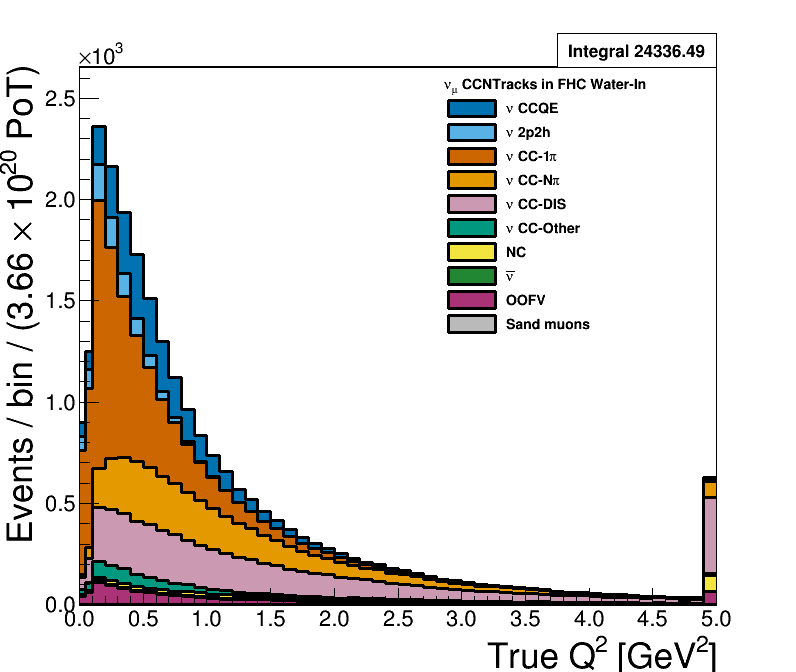
\includegraphics[width=0.45\textwidth]{Chapters/Figures/SamplesAndSelections/water/numu/CCNTracks/FluxAndEventWeights/numuCCNTracksWaterIn_trueQ2_MC_only_NEUTNuReactionCodes_fhc_water}
\par\end{centering}
}
\par\end{centering}
\begin{centering}
\subfloat[True $W$]{\begin{centering}
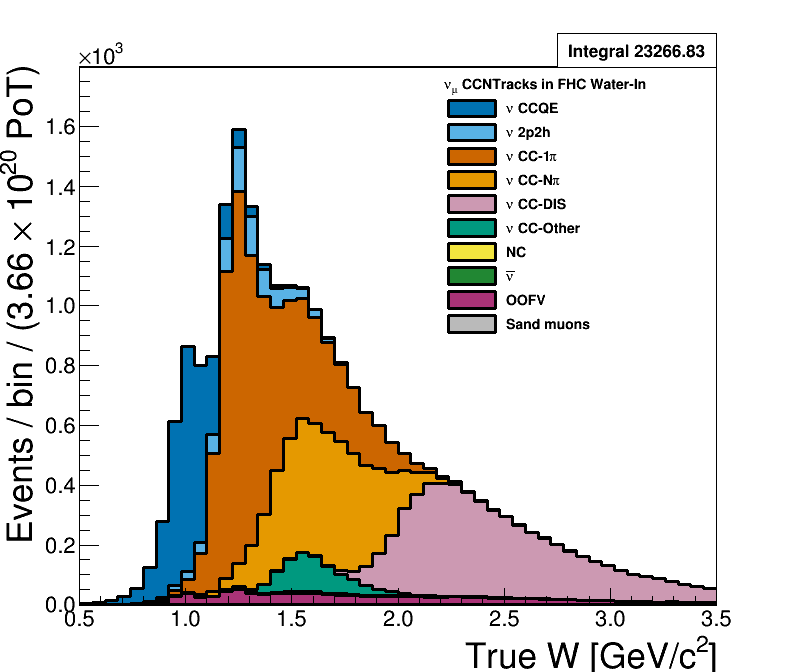
\includegraphics[width=0.45\textwidth]{Chapters/Figures/SamplesAndSelections/water/numu/CCNTracks/FluxAndEventWeights/numuCCNTracksWaterIn_trueW_MC_only_NEUTNuReactionCodes_fhc_water}
\par\end{centering}
}
\par\end{centering}
\caption[True Kinematics of the $\numu$ in FHC Mode CC N-Tracks Selection]{True kinematics of the $\protect\numu$ in FHC Mode CC N-Tracks selection.
The last bin shown in (a) and (b) is used as overflow. The figures
use the $\pod$ water-in MC and are normalized to the FHC water-in
mode POT. In figure (c), the largest resonance comes from the $\Delta$
baryon. There are higher order resonances in (c) as well.\label{fig:numuFHCCCNTrkTrue}}
\end{figure}

The origin of the mis-identified tracks, in particular the pion matched
tracks, becomes more clear since this is a high $Q^{2}$ selection.
The $N\pi$ and DIS events, which are high $Q^{2}$ events, can yield
a post-FSI charged pion track. These pions could have more energy
than the outgoing muon or could be the only particle observed in the
TPC.

\subsection{The \numubartitle{} in RHC Mode CC 1-Track Sample\label{subsec:numubarRHCCC1Trk}}

This selection provides the $\numubar$ CCQE-like samples in RHC mode
that are inputs to the BANFF fit. In \prettyref{fig:numubarRHCCC1TrkReco}
and \prettyref{fig:numubarRHCCC1TrkRecoParticle} display the momentum
and angular distributions for this selection. The selection is highly
$\numubar$-pure with the selected lepton candidate being positively
charged muons. There is a large OOFV background from proton tracks.
They are high momentum ($>1$ GeV/c) tracks which, at these energies,
are minimum ionizing and can reach into the TPC.

\begin{figure}[t]
\begin{centering}
\subfloat[Momentum]{\begin{centering}
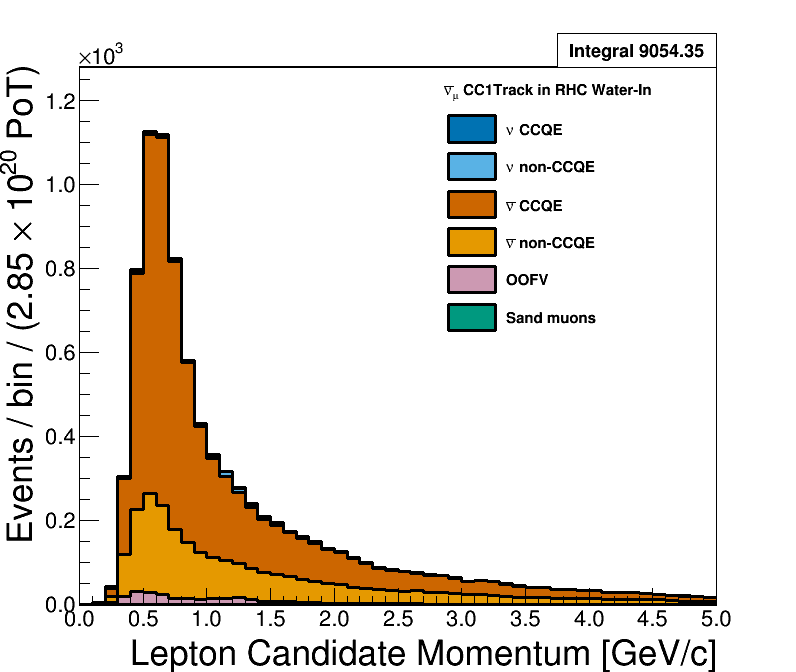
\includegraphics[width=0.45\textwidth]{Chapters/Figures/SamplesAndSelections/water/numubarRHC/CC1Track/FluxAndEventWeights/numubarRHCCC1TrackWaterIn_recoP_mu_MC_only_NEUTCCQELike_rhc_water}
\par\end{centering}
}\subfloat[$\cos\theta$]{\begin{centering}
`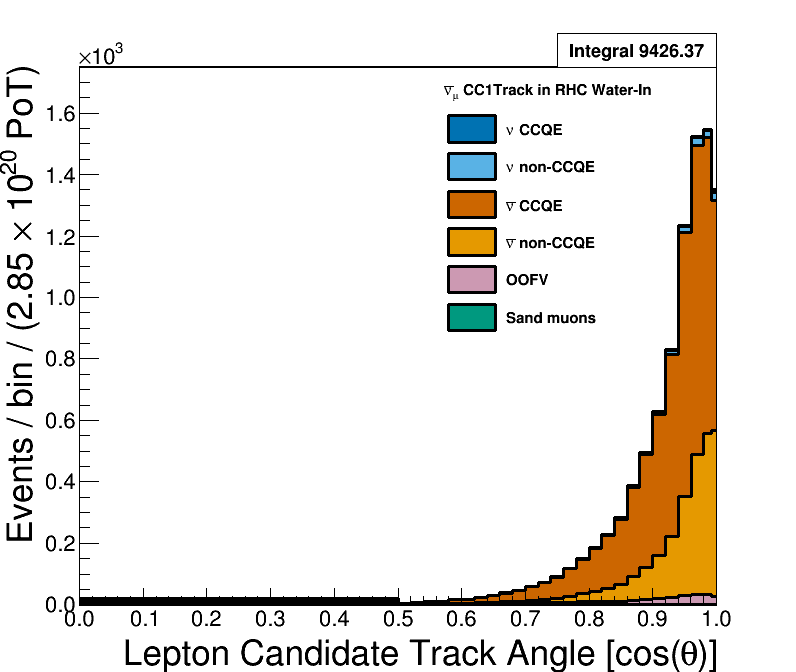
\includegraphics[width=0.45\textwidth]{Chapters/Figures/SamplesAndSelections/water/numubarRHC/CC1Track/FluxAndEventWeights/numubarRHCCC1TrackWaterIn_recocosq_mu_MC_only_NEUTCCQELike_rhc_water}
\par\end{centering}
}
\par\end{centering}
\caption[Reconstructed Kinematics of the $\numubar$ in RHC Mode CC 1-Track
Selection Categorized by CCQE and Non-CCQE Interactions]{Reconstructed kinematics of the $\protect\numubar$ in RHC Mode CC
1-Track selection categorized by CCQE and non-CCQE interactions. The
figures use the $\pod$ water-in MC and are normalized to the RHC
water-in mode POT. Also a single bin is used in the range of $0\protect\leq\cos\theta<0.5$
in figure (b).\label{fig:numubarRHCCC1TrkReco}}
\end{figure}

\begin{figure}
\begin{centering}
\subfloat[Water-in]{\begin{centering}
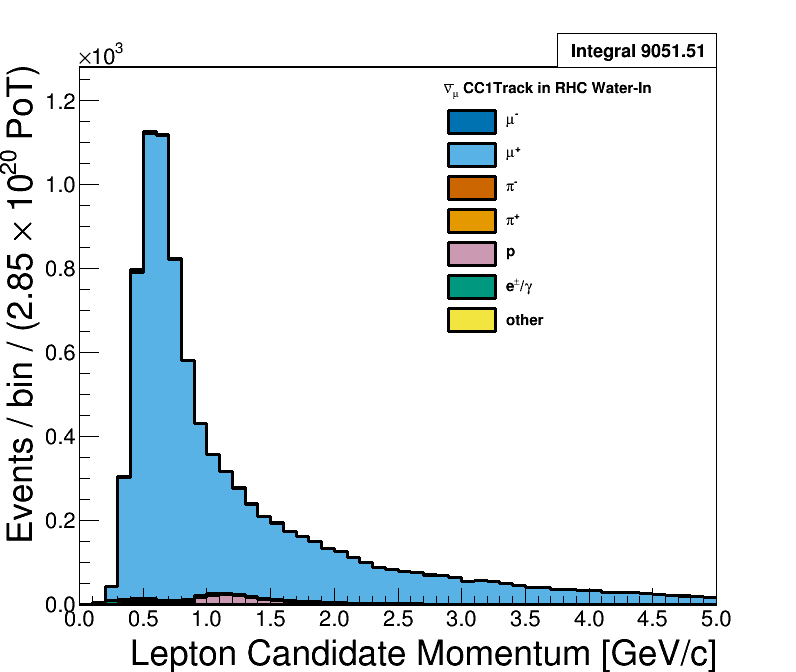
\includegraphics[width=0.45\textwidth]{Chapters/Figures/SamplesAndSelections/water/numubarRHC/CC1Track/FluxAndEventWeights/numubarRHCCC1TrackWaterIn_recoP_mu_MC_only_LeptonCandidateTruePDG_rhc_water}
\par\end{centering}
}\subfloat[Water-in]{\begin{centering}
`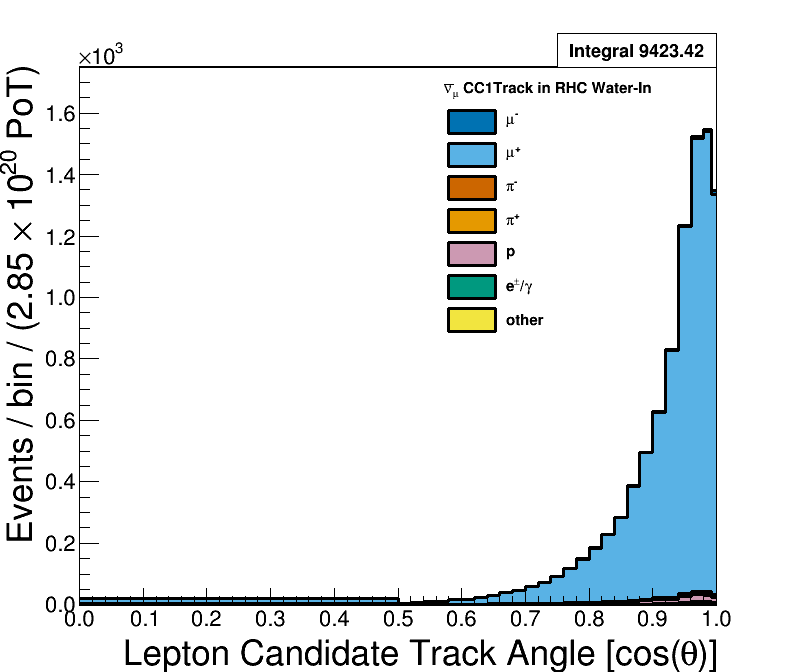
\includegraphics[width=0.45\textwidth]{Chapters/Figures/SamplesAndSelections/water/numubarRHC/CC1Track/FluxAndEventWeights/numubarRHCCC1TrackWaterIn_recocosq_mu_MC_only_LeptonCandidateTruePDG_rhc_water}
\par\end{centering}
}
\par\end{centering}
\caption[Reconstructed Kinematics of the $\numubar$ in RHC Mode CC 1-Track
Selection Categorized by the True Particle Matched to the Main Track]{Reconstructed kinematics of the $\protect\numubar$ in RHC Mode CC
1-Track selection categorized by the true particle matched to the
main track. The figures use the $\pod$ water-in MC and are normalized
to the RHC water-in mode POT. Also a single bin is used in the range
of $0\protect\leq\cos\theta<0.5$ in figure (b).\label{fig:numubarRHCCC1TrkRecoParticle}}
\end{figure}

We can examine the efficiencies and purities differentially for the
selection in \prettyref{fig:numubarRHCCC1TrkRecoEffPur}. For the
efficiency and purity only, the true signal is a true $\numubar$
CCQE interaction. The two distributions are very similar to the efficiency
and purity observed in the $\numu$ in FHC Mode CC 1-Track sample,
with the efficiency being relatively high (90\%) for high statistics
regions.

\begin{figure}
\begin{centering}
\subfloat[True $\protect\numubar$ CCQE Efficiency]{\begin{centering}
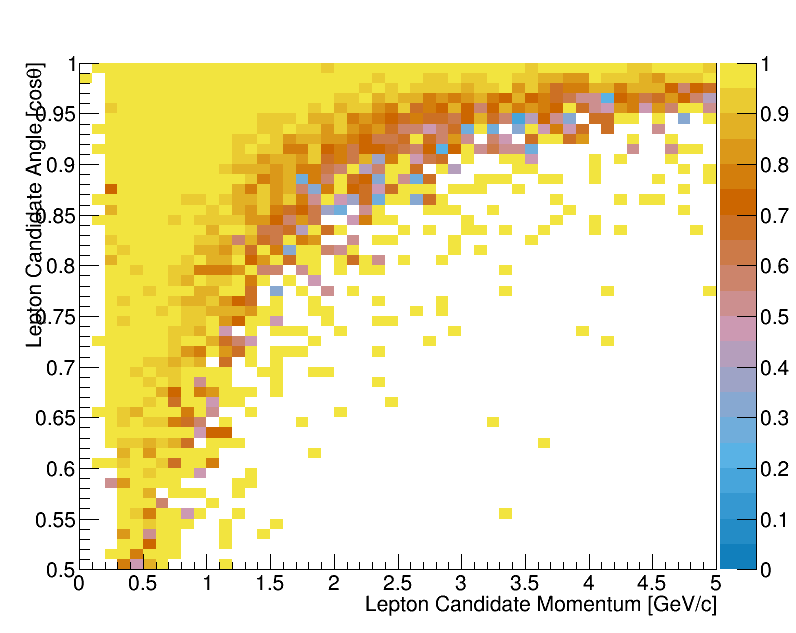
\includegraphics[width=0.45\textwidth]{Chapters/Figures/SamplesAndSelections/air/numubarRHC/CC1Track/FluxAndEventWeights/eff}
\par\end{centering}
}\subfloat[True $\protect\numubar$ CCQE Purity]{\begin{centering}
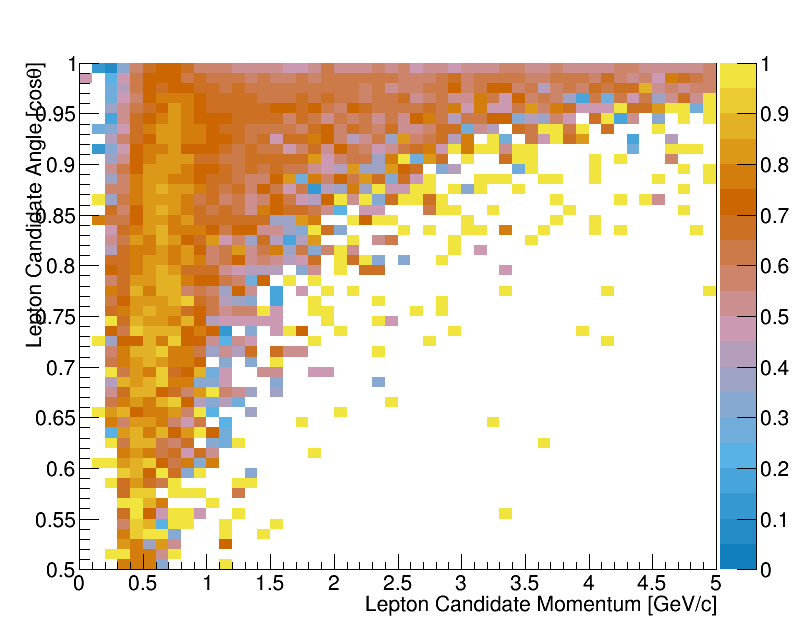
\includegraphics[width=0.45\textwidth]{Chapters/Figures/SamplesAndSelections/air/numubarRHC/CC1Track/FluxAndEventWeights/pur}
\par\end{centering}
}
\par\end{centering}
\caption[Efficiency and Purity of the $\numubar$ in RHC Mode CC 1-Track Selection]{Efficiency and purity of the $\protect\numubar$ in RHC Mode CC 1-Track
selection. The true events are $\protect\numubar$ CCQE at the vertex
and the selected lepton candidate is the true $\protect\muplus$.\label{fig:numubarRHCCC1TrkRecoEffPur}}
\end{figure}

The underlying true kinematics, $E_{\nu}$ and $Q^{2}$, of the interactions
are shown in \prettyref{fig:numubarRHCCC1TrkTrue}. We see a similar
true reaction composition with that of the $\numu$ in FHC Mode sample
in \mbox{Section~\ref{subsec:numuFHCCC1Trk}}. Most reactions are
true CCQE with a mixture of 2p2h and $1\pion$ events. As previously
seen in \mbox{Section~\ref{subsec:numuFHCCC1Trk}}, the significant
$1\pi$ contamination may reduce the sensitivity to both CC-$0\pi$
and CC-$1\pi$ model parameters in the BANFF fit.

\begin{figure}
\begin{centering}
\subfloat[True Neutrino Energy]{\begin{centering}
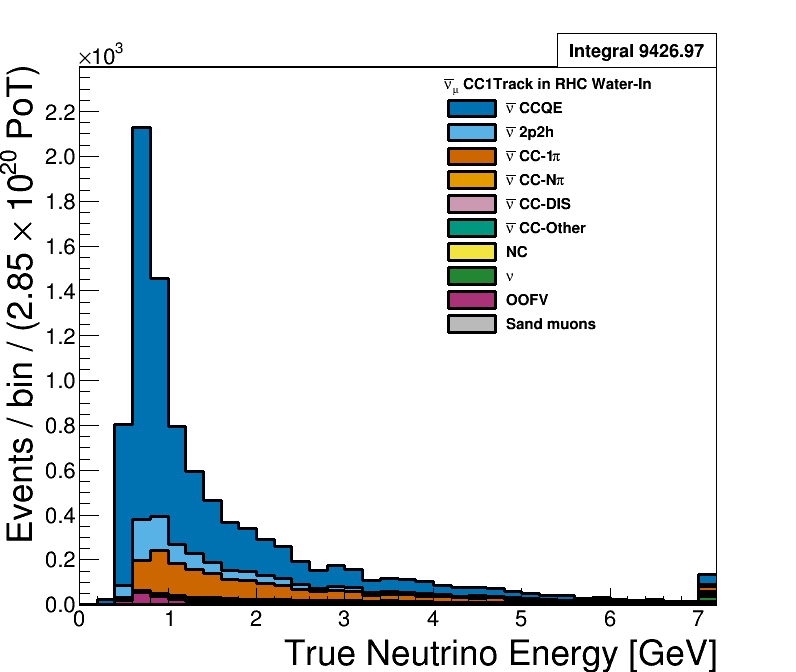
\includegraphics[width=0.45\textwidth]{Chapters/Figures/SamplesAndSelections/water/numubarRHC/CC1Track/FluxAndEventWeights/numubarRHCCC1TrackWaterIn_trueE_nu_MC_only_NEUTAntiNuReactionCodes_rhc_water}
\par\end{centering}
}\subfloat[True $Q^{2}$]{\begin{centering}
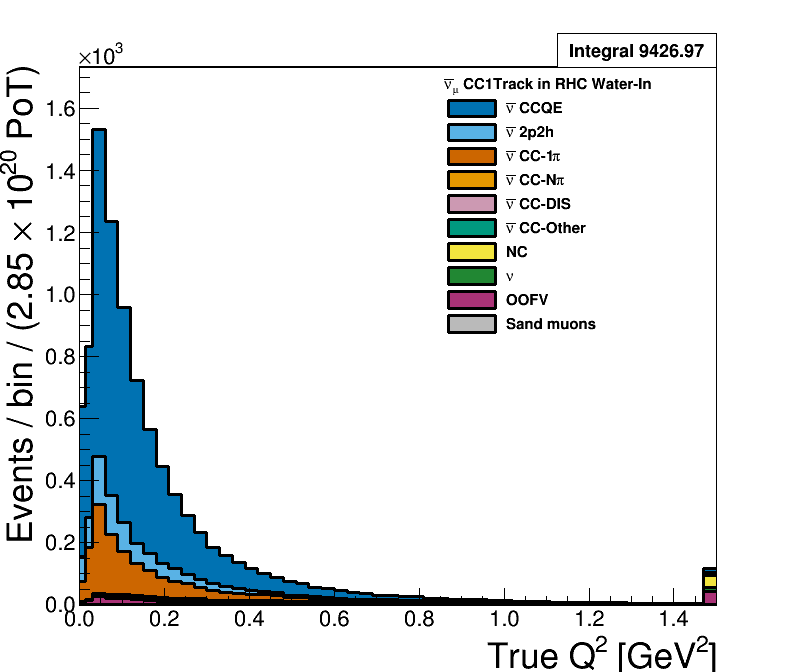
\includegraphics[width=0.45\textwidth]{Chapters/Figures/SamplesAndSelections/water/numubarRHC/CC1Track/FluxAndEventWeights/numubarRHCCC1TrackWaterIn_trueQ2_MC_only_NEUTAntiNuReactionCodes_rhc_water}
\par\end{centering}
}
\par\end{centering}
\caption[True Kinematics of the $\numubar$ in RHC Mode CC 1-Track Selection]{True kinematics of the $\protect\numubar$ in RHC Mode CC 1-Track
selection. Water-in mode is displayed here only with the last bin
shown is used as overflow. The figures use the $\pod$ water-in MC
and are normalized to the RHC water-in mode POT.\label{fig:numubarRHCCC1TrkTrue}}
\end{figure}


\subsection{The \numubartitle{} in RHC Mode CC N-Tracks Sample}

This selection provides the $\numubar$ non-CCQE-like samples in RHC
mode. \prettyref{fig:numubarRHCCCNTrkReco} and \prettyref{fig:numubarRHCCCNTrkRecoParticle}
display the momentum and angular distributions that are inputs to
BANFF. The most striking feature of this selection is the number of
mis-identified events. In particular tracks matched to protons are
selected as the HMPT when the protons are minimum ionizing particles
themselves, which is about $1.3$ GeV/c. In addition, the intrinsic
$\numu$ background contribution is comparable to the desired $\numubar$
flavor. These two features should be addressed to increase the utility
of the selection for the next iteration of the analysis.

\begin{figure}
\begin{centering}
\subfloat[Momentum]{\begin{centering}
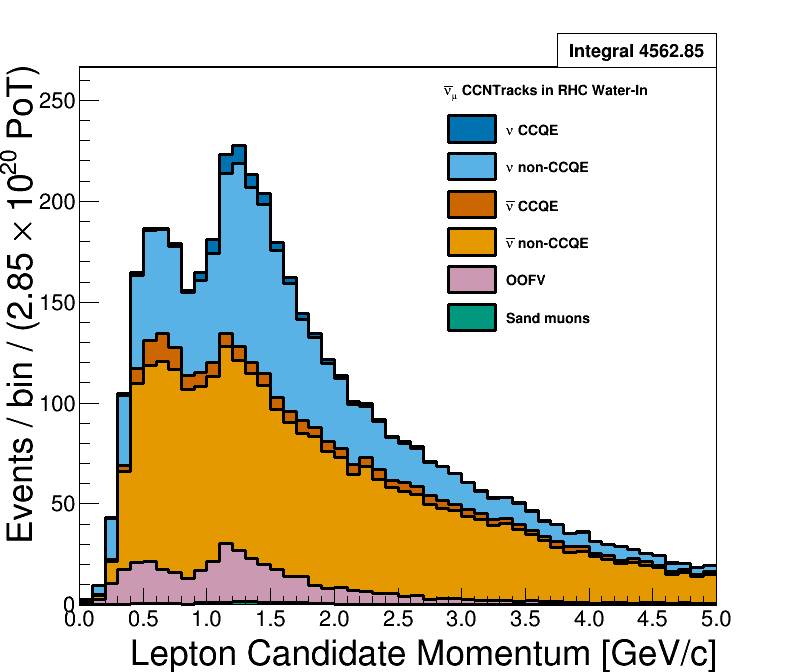
\includegraphics[width=0.45\textwidth]{Chapters/Figures/SamplesAndSelections/water/numubarRHC/CCNTracks/FluxAndEventWeights/numubarRHCCCNTracksWaterIn_recoP_mu_MC_only_NEUTCCQELike_rhc_water}
\par\end{centering}
}\subfloat[$\cos\theta$]{\begin{centering}
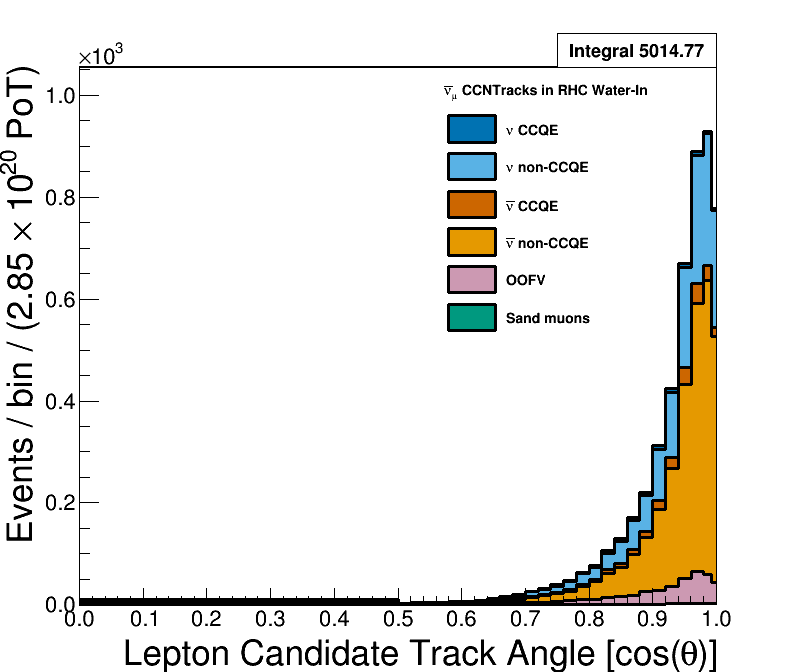
\includegraphics[width=0.45\textwidth]{Chapters/Figures/SamplesAndSelections/water/numubarRHC/CCNTracks/FluxAndEventWeights/numubarRHCCCNTracksWaterIn_recocosq_mu_MC_only_NEUTCCQELike_rhc_water}
\par\end{centering}
}
\par\end{centering}
\caption[Reconstructed Kinematics of the $\numubar$ in RHC Mode CC N-Tracks
Selection Categorized by CCQE and Non-CCQE Interactions]{Reconstructed kinematics of the $\protect\numubar$ in RHC Mode CC
N-Tracks selection categorized by CCQE and non-CCQE interactions.
The figures use the $\pod$ water-in MC and are normalized to the
RHC water-in mode POT. Also a single bin is used in the range of $0\protect\leq\cos\theta<0.5$
in figure (b).\label{fig:numubarRHCCCNTrkReco}}
\end{figure}

\begin{figure}
\begin{centering}
\subfloat[Momentum]{\begin{centering}
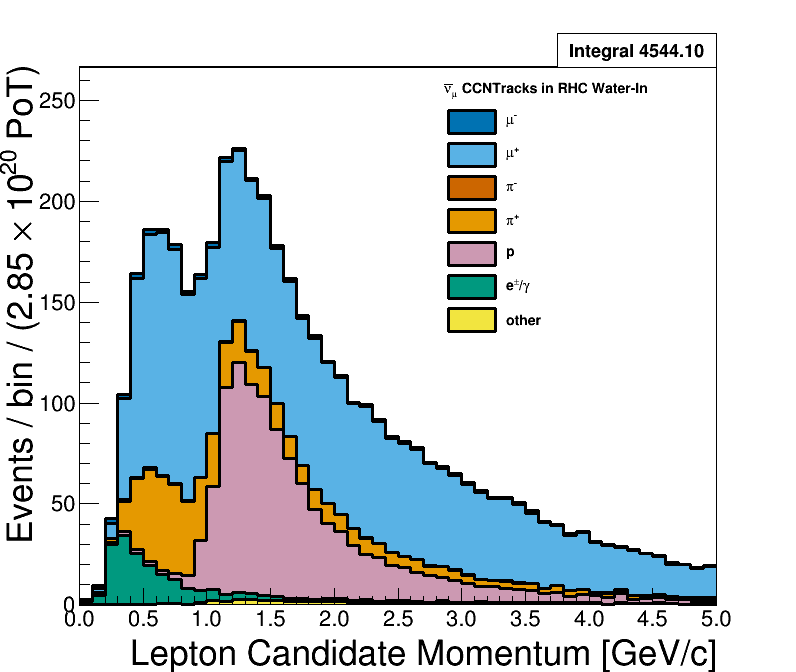
\includegraphics[width=0.45\textwidth]{Chapters/Figures/SamplesAndSelections/water/numubarRHC/CCNTracks/FluxAndEventWeights/numubarRHCCCNTracksWaterIn_recoP_mu_MC_only_LeptonCandidateTruePDG_rhc_water}
\par\end{centering}
}\subfloat[$\cos\theta$]{\begin{centering}
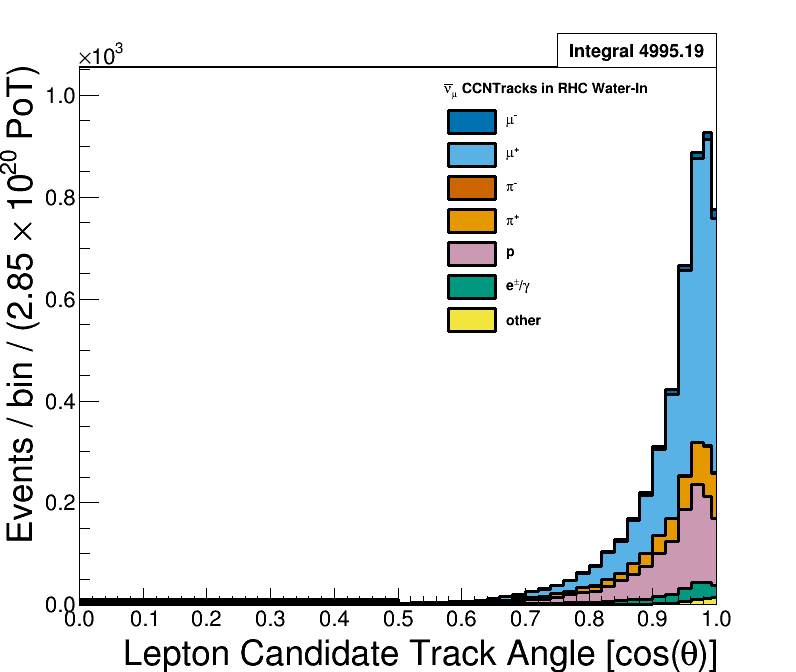
\includegraphics[width=0.45\textwidth]{Chapters/Figures/SamplesAndSelections/water/numubarRHC/CCNTracks/FluxAndEventWeights/numubarRHCCCNTracksWaterIn_recocosq_mu_MC_only_LeptonCandidateTruePDG_rhc_water}
\par\end{centering}
}
\par\end{centering}
\caption[Reconstructed Kinematics of the $\numubar$ in RHC Mode CC N-Tracks
Selection Categorized by the True Particle Matched to the Main Track]{Reconstructed kinematics of the $\protect\numubar$ in RHC Mode CC
N-Tracks selection categorized by the true particle matched to the
main track. The figures use the $\pod$ water-in MC and are normalized
to the RHC water-in mode POT. Also a single bin is used in the range
of $0\protect\leq\cos\theta<0.5$ in figure (b).\label{fig:numubarRHCCCNTrkRecoParticle}}
\end{figure}

We can examine the efficiencies and purities differentially for the
selection in \prettyref{fig:numuFHCCCNTrkRecoEffPur}. For the efficiency
and purity only, the true signal is any $\numubar$ CC interaction
except $\numubar$ CCQE which the CC 1-Track selection is designed
to select. Both the efficiency and purity are low where statistics
are high due to the wrong sign background.

\begin{figure}
\begin{centering}
\subfloat[True $\protect\numubar$ CC non-QE Efficiency]{\begin{centering}
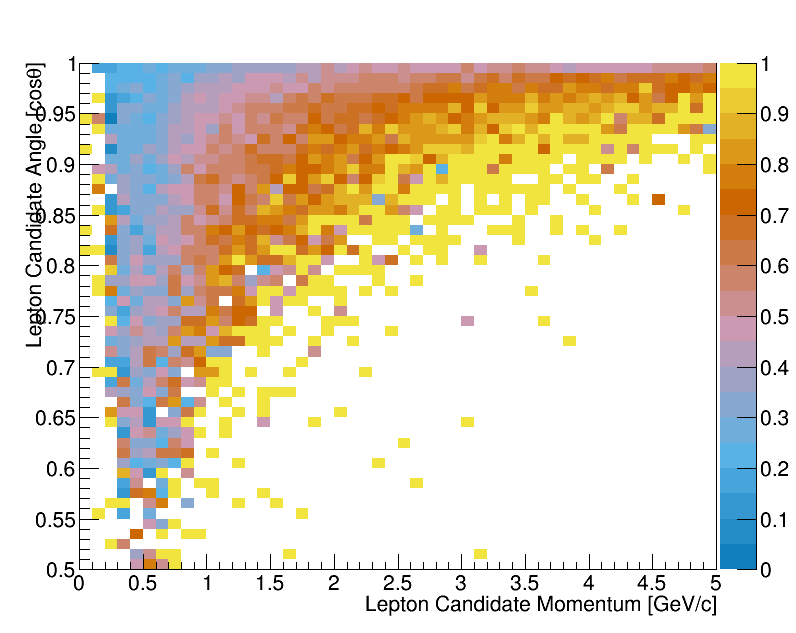
\includegraphics[width=0.45\textwidth]{Chapters/Figures/SamplesAndSelections/air/numubarRHC/CCNTracks/FluxAndEventWeights/eff}
\par\end{centering}
}\subfloat[True $\protect\numubar$ CC non-QE Purity]{\begin{centering}
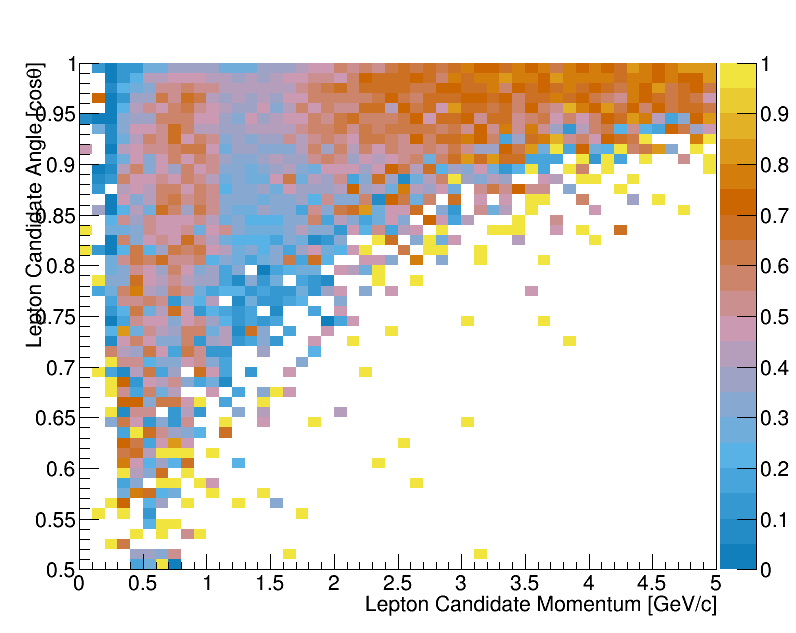
\includegraphics[width=0.45\textwidth]{Chapters/Figures/SamplesAndSelections/air/numubarRHC/CCNTracks/FluxAndEventWeights/pur}
\par\end{centering}
}
\par\end{centering}
\caption[Efficiency and Purity of the $\numubar$ in RHC Mode CC N-Tracks Selection]{Efficiency and purity of the $\protect\numubar$ in RHC Mode CC N-Tracks
selection. True events are defined as correctly matched $\protect\muplus$
tracks from $\protect\numubar$-induced CC non-QE interactions at
the vertex. \label{fig:numubarRHCCCNTrkRecoEffPur}}
\end{figure}

The underlying true kinematics, $E_{\nu}$, $Q^{2}$, and $W$, of
the interactions are shown in \prettyref{fig:numubarRHCCCNTrkTrue}.
Here we see in better detail the origin of the $\numu$ contamination.
As a function of increasing energy, the $\numubar$ content is decreasing
while the relative $\numu$ contribution is increasing. The $\numu$
events also have high $Q^{2}$ which explains the significant number
of misidentified proton main track events. For the hadronic final
states, the shape of the $\numubar$-induced resonances is similar
to what we saw in \prettyref{fig:numuFHCCCNTrkTrue}. Interestingly,
the $\numu$ background hadronic mass distribution does not peak in
any one region.

\begin{figure}
\begin{centering}
\subfloat[True Neutrino Energy]{\begin{centering}
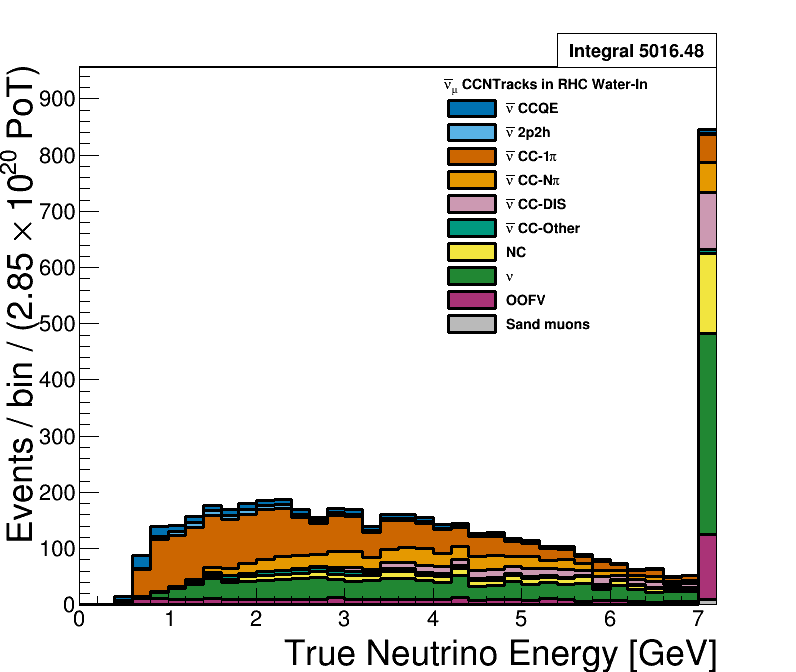
\includegraphics[width=0.45\textwidth]{Chapters/Figures/SamplesAndSelections/water/numubarRHC/CCNTracks/FluxAndEventWeights/numubarRHCCCNTracksWaterIn_trueE_nu_MC_only_NEUTAntiNuReactionCodes_rhc_water}
\par\end{centering}
}\subfloat[True $Q^{2}$]{\begin{centering}
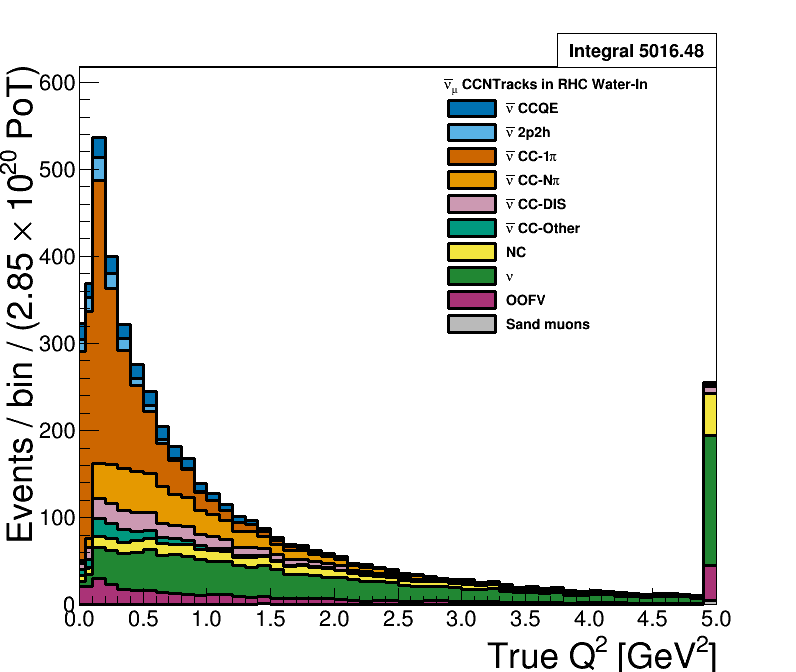
\includegraphics[width=0.45\textwidth]{Chapters/Figures/SamplesAndSelections/water/numubarRHC/CCNTracks/FluxAndEventWeights/numubarRHCCCNTracksWaterIn_trueQ2_MC_only_NEUTAntiNuReactionCodes_rhc_water}
\par\end{centering}
}
\par\end{centering}
\begin{centering}
\subfloat[True $W$]{\begin{centering}
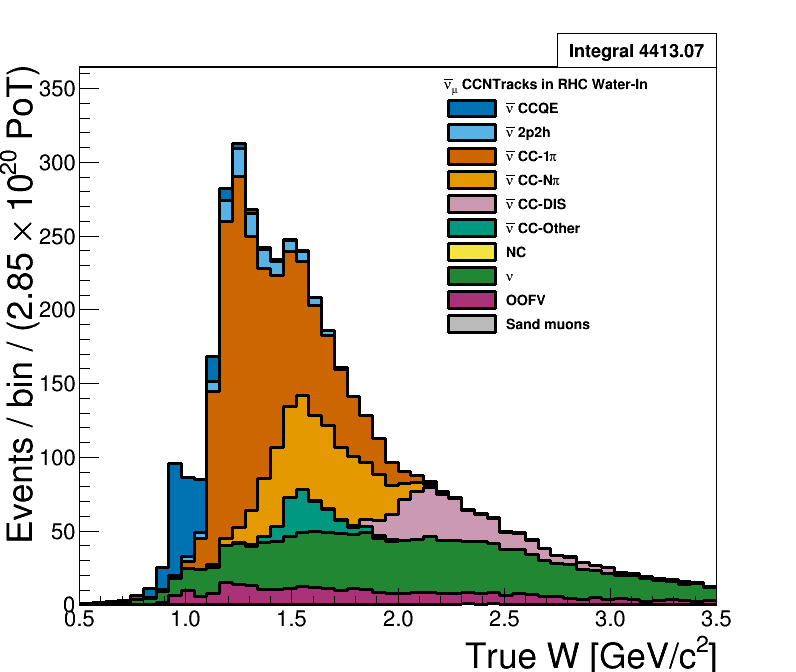
\includegraphics[width=0.45\textwidth]{Chapters/Figures/SamplesAndSelections/water/numubarRHC/CCNTracks/FluxAndEventWeights/numubarRHCCCNTracksWaterIn_trueW_MC_only_NEUTAntiNuReactionCodes_rhc_water}
\par\end{centering}
}
\par\end{centering}
\caption[True Kinematics of the $\numubar$ in RHC Mode CC N-Tracks Selection]{True kinematics of the $\protect\numubar$ in RHC Mode CC N-Tracks
selection. The last bin shown in (a) and (b) is used as overflow.
The figures use the $\pod$ water-in MC and are normalized to the
RHC water-in mode POT. \label{fig:numubarRHCCCNTrkTrue}}
\end{figure}


\subsection{The \numutitle{} Background in RHC Mode CC 1-Track Sample}

This selection provides the $\numu$ in RHC, also called wrong-sign
background, CCQE-like samples . \prettyref{fig:numuRHCCC1TrkReco}
and \prettyref{fig:numuRHCCC1TrkRecoParticle} display the momentum
and angular distributions inputs to the BANFF fit. We can see this
is a relatively low-angle selection compared to previous selections.
Importantly the selection is relatively $\numu$-pure which should
help constrain the wrong-sign background in the fit. However, the
CCQE purity is modest given number of correctly identified lepton
candidates. This feature needs to be addressed in the next iteration
of the analysis.

\begin{figure}
\begin{centering}
\subfloat[Momentum]{\begin{centering}
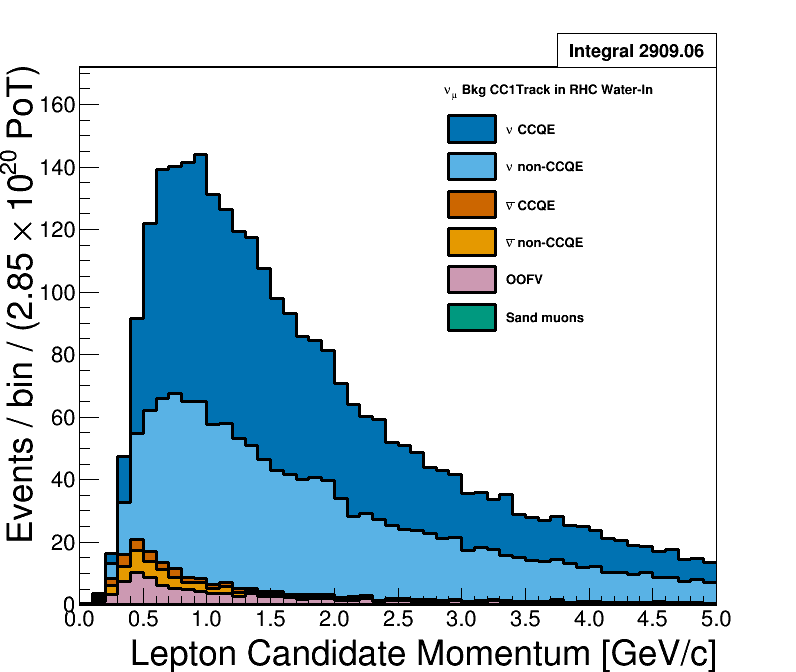
\includegraphics[width=0.45\textwidth]{Chapters/Figures/SamplesAndSelections/water/numubkgRHC/CC1Track/FluxAndEventWeights/numubkgRHCCC1TrackWaterIn_recoP_mu_MC_only_NEUTCCQELike_rhc_water}
\par\end{centering}
}\subfloat[$\cos\theta$]{\begin{centering}
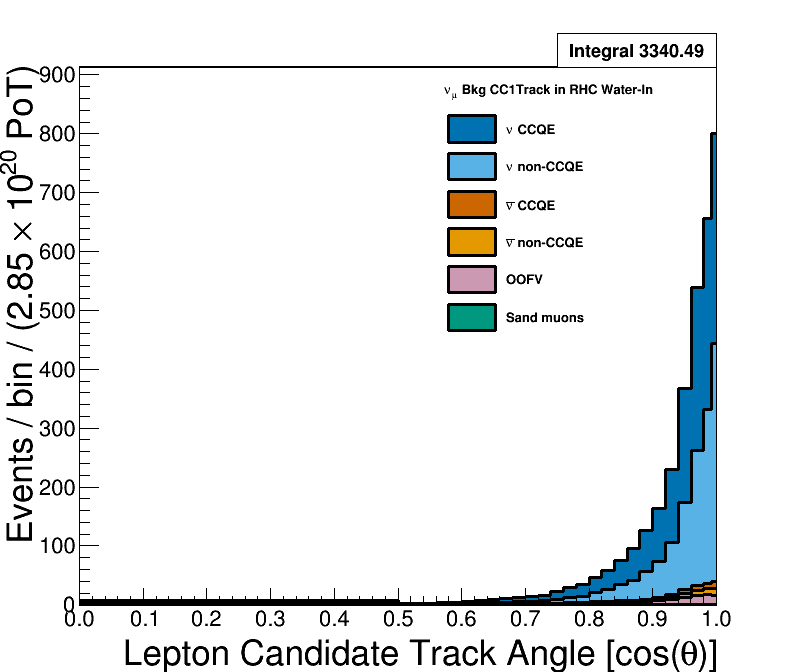
\includegraphics[width=0.45\textwidth]{Chapters/Figures/SamplesAndSelections/water/numubkgRHC/CC1Track/FluxAndEventWeights/numubkgRHCCC1TrackWaterIn_recocosq_mu_MC_only_NEUTCCQELike_rhc_water}
\par\end{centering}
}
\par\end{centering}
\caption[Reconstructed Kinematics of the $\numu$ Background in RHC Mode CC
1-Track Selection Categorized by CCQE and Non-CCQE Interactions]{Reconstructed kinematics of the $\protect\numu$ Background in RHC
Mode CC 1-Track selection categorized by CCQE and non-CCQE interactions.
The figures use the $\pod$ water-in MC and are normalized to the
RHC water-in mode POT. Also a single bin is used in the range of $0\protect\leq\cos\theta<0.5$
in figure (b).\label{fig:numuRHCCC1TrkReco}}
\end{figure}

\begin{figure}
\begin{centering}
\subfloat[Momentum]{\begin{centering}
\includegraphics[width=0.45\textwidth]{Chapters/Figures/SamplesAndSelections/water/numubkgRHC/CC1Track/FluxAndEventWeights/numubkgRHCCC1TrackWaterIn_recoP_mu_MC_only_LeptonCandidateTruePDG_rhc_water}
\par\end{centering}
}\subfloat[$\cos\theta$]{\begin{centering}
\includegraphics[width=0.45\textwidth]{Chapters/Figures/SamplesAndSelections/water/numubkgRHC/CC1Track/FluxAndEventWeights/numubkgRHCCC1TrackWaterIn_recocosq_mu_MC_only_LeptonCandidateTruePDG_rhc_water}
\par\end{centering}
}
\par\end{centering}
\caption[Reconstructed Kinematics of the $\numu$ Background in RHC Mode CC
1-Track Selection Categorized by the True Particle Matched to the
Main Track]{Reconstructed kinematics of the $\protect\numu$ Background in RHC
Mode CC 1-Track selection categorized by the true particle matched
to the main track. The figures use the $\pod$ water-in MC and are
normalized to the RHC water-in mode POT. Also a single bin is used
in the range of $0\protect\leq\cos\theta<0.5$ in figure (b).\label{fig:numuRHCCC1TrkRecoParticle}}
\end{figure}

We can examine the efficiencies and purities differentially for the
selection in \prettyref{fig:numuRHCCC1TrkRecoEffPur}. For the efficiency
and purity only, the true signal is a true $\numu$ CCQE interaction.
The efficiency is similar to the $\numu$ in FHC Mode CC 1-Track topology
efficiency with banded $p-\theta$ regions. As for the purity, it
is roughly 70\% in a banded region between low momenta, low angle
and high momenta, high angle tracks.

\begin{figure}
\begin{centering}
\subfloat[True $\protect\numu$ CCQE Efficiency]{\begin{centering}
\includegraphics[width=0.45\textwidth]{Chapters/Figures/SamplesAndSelections/air/numubkgRHC/CC1Track/FluxAndEventWeights/eff}
\par\end{centering}
}\subfloat[True $\protect\numu$ CCQE Purity]{\begin{centering}
\includegraphics[width=0.45\textwidth]{Chapters/Figures/SamplesAndSelections/air/numubkgRHC/CC1Track/FluxAndEventWeights/pur}
\par\end{centering}
}
\par\end{centering}
\caption[Efficiency and Purity of the $\numu$ Background in RHC Mode CC 1-Track
Selection]{Efficiency and purity of the $\protect\numu$ Background in RHC Mode
CC 1-Track selection. The true events are $\protect\numu$ CCQE at
the vertex and the selected lepton candidate is the true $\protect\muminus$.
\label{fig:numuRHCCC1TrkRecoEffPur}}
\end{figure}

The underlying true kinematics, $E_{\nu}$ and $Q^{2}$, of the selection
are shown in \prettyref{fig:numuRHCCC1TrkTrue}. The number of the
wrong-sign background events peaks at 1 GeV and is a broad peak compared
to the designed sharp $\numubar$ peak at 0.6 GeV as shown in \prettyref{fig:numubarRHCCC1TrkTrue}.
Since these are higher energy events, there is more available energy
to produce resonance states that produce $1\pi$ topologies. This
explains the significant non-CCQE event contamination.

\begin{figure}
\begin{centering}
\subfloat[True Neutrino Energy]{\begin{centering}
\includegraphics[width=0.45\textwidth]{Chapters/Figures/SamplesAndSelections/water/numubkgRHC/CC1Track/FluxAndEventWeights/numubkgRHCCC1TrackWaterIn_trueE_nu_MC_only_NEUTNuReactionCodes_rhc_water}
\par\end{centering}
}\subfloat[True $Q^{2}$]{\begin{centering}
\includegraphics[width=0.45\textwidth]{Chapters/Figures/SamplesAndSelections/water/numubkgRHC/CC1Track/FluxAndEventWeights/numubkgRHCCC1TrackWaterIn_trueQ2_MC_only_NEUTNuReactionCodes_rhc_water}
\par\end{centering}
}
\par\end{centering}
\caption[True Kinematics of the $\numu$ Background in RHC Mode CC 1-Track
Selection]{True kinematics of the $\protect\numu$ Background in RHC Mode CC
1-Track selection. Water-in mode is displayed here only with the last
bin shown is used as overflow. The figures use the $\pod$ water-in
MC and are normalized to the RHC water-in mode POT.\label{fig:numuRHCCC1TrkTrue}}
\end{figure}


\subsection{The \numutitle{} Background in RHC Mode CC N-Tracks Sample}

This selection provides the non-CCQE-like samples for the $\numu$
background in RHC mode. \prettyref{fig:numuRHCCCNTrkReco} and \prettyref{fig:numuRHCCCNTrkRecoParticle}
show the momentum and angular distributions that are inputs to the
BANFF fit. We can see the selection is relatively $\numu$-pure with
a significant mis-identified track rate. Interestingly, the misidentified
pion main tracks have a high momentum tail.

\begin{figure}
\begin{centering}
\subfloat[Momentum]{\begin{centering}
\includegraphics[width=0.45\textwidth]{Chapters/Figures/SamplesAndSelections/water/numubkgRHC/CCNTracks/FluxAndEventWeights/numubkgRHCCCNTracksWaterIn_recoP_mu_MC_only_NEUTCCQELike_rhc_water}
\par\end{centering}
}\subfloat[$\cos\theta$]{\begin{centering}
\includegraphics[width=0.45\textwidth]{Chapters/Figures/SamplesAndSelections/water/numubkgRHC/CCNTracks/FluxAndEventWeights/numubkgRHCCCNTracksWaterIn_recocosq_mu_MC_only_NEUTCCQELike_rhc_water}
\par\end{centering}
}
\par\end{centering}
\caption[Reconstructed Kinematics of the $\numu$ Background in RHC Mode CC
N-Tracks Selection Categorized by CCQE and Non-CCQE Interactions]{Reconstructed kinematics of the $\protect\numu$ Background in RHC
Mode CC 1-Track selection categorized by CCQE and non-CCQE interactions.
The figures use the $\pod$ water-in MC and are normalized to the
RHC water-in mode POT. Also a single bin is used in the range of $0\protect\leq\cos\theta<0.5$
in figure (b).\label{fig:numuRHCCCNTrkReco}}
\end{figure}

\begin{figure}
\begin{centering}
\subfloat[Momentum]{\begin{centering}
\includegraphics[width=0.45\textwidth]{Chapters/Figures/SamplesAndSelections/water/numubkgRHC/CCNTracks/FluxAndEventWeights/numubkgRHCCCNTracksWaterIn_recoP_mu_MC_only_LeptonCandidateTruePDG_rhc_water}
\par\end{centering}
}\subfloat[$\cos\theta$]{\begin{centering}
\includegraphics[width=0.45\textwidth]{Chapters/Figures/SamplesAndSelections/water/numubkgRHC/CCNTracks/FluxAndEventWeights/numubkgRHCCCNTracksWaterIn_recocosq_mu_MC_only_LeptonCandidateTruePDG_rhc_water}
\par\end{centering}
}
\par\end{centering}
\caption[Reconstructed Kinematics of the $\numu$ Background in RHC Mode CC
N-Tracks Selection Categorized by the True Particle Matched to the
Main Track]{Reconstructed kinematics of the $\protect\numu$ Background in RHC
Mode CC 1-Track selection categorized by the true particle matched
to the main track. The figures use the $\pod$ water-in MC and are
normalized to the RHC water-in mode POT. Also a single bin is used
in the range of $0\protect\leq\cos\theta<0.5$ in figure (b).\label{fig:numuRHCCCNTrkRecoParticle}}
\end{figure}

We can examine the $\numu$ CC non-QE efficiency and purity of the
selection in \prettyref{fig:numuRHCCCNTrkRecoEffPur}. There is a
reduction in the purity below 1.5 GeV/c due to the the $\numubar$
selections occupying the same phase space. Fortunately, the efficiency
and purity are relatively high above 1.5 GeV/c.

\begin{figure}
\begin{centering}
\subfloat[True $\protect\numu$ CC non-QE Efficiency]{\begin{centering}
\includegraphics[width=0.45\textwidth]{/home/mhogan/Documents/graduateDisseration/Chapters/Figures/SamplesAndSelections/air/numubkgRHC/CCNTracks/FluxAndEventWeights/eff}
\par\end{centering}
}\subfloat[True $\protect\numu$ CC non-QE Purity]{\begin{centering}
\includegraphics[width=0.45\textwidth]{/home/mhogan/Documents/graduateDisseration/Chapters/Figures/SamplesAndSelections/air/numubkgRHC/CCNTracks/FluxAndEventWeights/pur}
\par\end{centering}
}
\par\end{centering}
\caption[Efficiency and Purity of the $\numu$ Background in RHC Mode CC N-Tracks
Selection]{Efficiency and purity of the $\protect\numu$ Background in RHC Mode
CC N-Tracks selection. True events are defined as correctly matched
$\protect\muminus$ tracks from $\protect\numu$-induced CC non-QE
interactions at the vertex. \label{fig:numuRHCCCNTrkRecoEffPur}}
\end{figure}

The underlying true kinematics, $E_{\nu}$, $Q^{2}$, and $W$, of
the interactions are shown in \prettyref{fig:numuRHCCCNTrkTrue}.
As we have seen before with the CC N-Tracks samples, these are high
$E_{\nu}$ events with large $Q^{2}$ exchanges. The invariant hadronic
system displays the previously seen resonances, with the largest still
being from the $\Delta$ baryon.

\begin{figure}
\begin{centering}
\subfloat[True Neutrino Energy]{\begin{centering}
\includegraphics[width=0.45\textwidth]{Chapters/Figures/SamplesAndSelections/water/numubkgRHC/CCNTracks/FluxAndEventWeights/numubkgRHCCCNTracksWaterIn_trueE_nu_MC_only_NEUTNuReactionCodes_rhc_water}
\par\end{centering}
}\subfloat[True $Q^{2}$]{\begin{centering}
\includegraphics[width=0.45\textwidth]{Chapters/Figures/SamplesAndSelections/water/numubkgRHC/CCNTracks/FluxAndEventWeights/numubkgRHCCCNTracksWaterIn_trueQ2_MC_only_NEUTNuReactionCodes_rhc_water}
\par\end{centering}
}
\par\end{centering}
\begin{centering}
\subfloat[True $W$]{\begin{centering}
\includegraphics[width=0.45\textwidth]{Chapters/Figures/SamplesAndSelections/water/numubkgRHC/CCNTracks/FluxAndEventWeights/numubkgRHCCCNTracksWaterIn_trueW_MC_only_NEUTNuReactionCodes_rhc_water}
\par\end{centering}
}
\par\end{centering}
\caption[True Kinematics of the $\numu$ Background in RHC Mode CC N-Tracks
Selection]{True kinematics of the $\protect\numu$ Background in RHC Mode CC
N-Tracks selection. The last bin shown in (a) and (b) is used as overflow.
The figures use the $\pod$ water-in MC and are normalized to the
RHC water-in mode POT. \label{fig:numuRHCCCNTrkTrue}}
\end{figure}


\section{Summary\label{sec:SelectionSummary}}

In this chapter we have examined the selection true and reconstruction
kinematics that will used in the BANFF fit. We see the 1-Track selections
yield some reasonably pure CCQE samples. By inverting that cut, we
obtain some information on the rate of other topologies like CC-$1\pi$
and high $Q^{2}$ CCDIS events. Importantly is the ability of these
samples to constrain the correct sign ($\numubar$) and wrong sign
($\numu$) backgrounds in RHC mode, which are very important in the
oscillation analysis. We can now move forward to the next chapter
to describe the fit parameters and the systematic uncertainties present
in the analysis.



\chapter{The BANFF Fit Parameters\label{chap:P0DinBANFF}}

This chapter explores the fit binning and penalty terms in the test
statistic used for this analysis. The BANFF fit includes three sources
of systematic uncertainties: neutrino flux, cross section model, and
detector inefficiencies. The sources of systematic uncertainty, also
referred to just as systematics, will be defined and their effects
on the analysis will be examined. These three terms directly affect
the flux of neutrinos, efficiency of reconstruction, and the cross
section for $\nu_{\alpha}$ terms, respectively, in the predicted
rate equation given in \eqref{eq:Nsig}. 

This chapter is presented in the following order. The method to define
histogram fit bins in the likelihood ratio is discussed in \prettyref{sec:Fit-Binning}.
The parameterization of each penalty term in the test statistic is
described in \prettyref{sec:Systematic-Uncertainties-and} in the
following order: the neutrino flux model, the detector inefficiencies,
and the cross section model. The chapter summary is provided in \prettyref{sec:ParameterizationSummary}.


\section{Fit Binning\label{sec:Fit-Binning}}

The $\pod$-only BANFF fit uses the samples described in \prettyref{chap:P0DSelections}
to evaluate the log-likelihood ratio term, $\chi_{\text{LLR}}^{2}$.
Since this is a binned likelihood in $(p,\cos\theta)$, the bin edges
need to be defined first.

The BANFF fit binning is optimized to ensure at least 1 predicted
Monte Carlo (MC) event in each bin for every $\pod$ sample when scaled
to the collected data POT. The fit bins must also account for detector
smearing effects. In order to mitigate smearing and event migration,
the reconstructed muon track kinematics were examined against correctly
identified tracks in one-dimensional kinematic slices. The kinematics
are scanned across their full phase spaces in order to understand
the required width for a fit bin. The first fit bin is always defined
starting from the kinematic maximum.

To determine the optimal momentum fit bins, the momentum resolution
with the MC truth matched muon is analyzed. The momentum resolution
is defined as
\[
R(r,t)=\frac{r-t}{t},
\]
where $r$ is the reconstructed momentum and $t$ is the true muon
momentum. The mean (bias) and standard deviation (stddev) of $R$
are used as proxies for the true bias and resolution for the prediction.
Both quantities and prediction errors were extracted using a bootstrapping
algorithm\cite{springer_series978-0-387-84858-7} in very fine bins
of reconstructed momentum. The bootstrapping algorithm works by random
sampling with replacement of the true muon momentum. For each bias
and stddev prediction, at least 1000 bootstrapping samples were generated.
Each bootstrap bias and stddev value were saved to calculate a prediction
mean and error. In the case of relatively ``large'' prediction errors,
additional 10000 bootstrapping samples were generated. The main track
momentum resolution for the $\numu$ in FHC Mode CC 1-Track sample
is shown in \prettyref{fig:MomentumKinematicsBootstrappingNumuCC1Track}
to illustrate the results.

\begin{figure}
\begin{centering}
\subfloat[Momentum distribution]{\centering{}\includegraphics[width=0.48\textwidth]{Chapters/Figures/P0DBANFFParameterization/MomentumKinematicsNumuCC1Track}}\subfloat[Momentum resolution]{\centering{}\includegraphics[width=0.45\textwidth]{Chapters/Figures/P0DBANFFParameterization/MomentumKinematicsUncertaintiesNumuCC1Track}}
\par\end{centering}
\caption[Main Track Momentum Resolution for the $\numu$ in FHC Mode CC 1-Track
Sample]{Main track momentum resolution for the $\protect\numu$ in FHC Mode
CC 1-Track sample. Only correctly identified muons are used. The number
of events is scaled to $10^{20}$ POT, which is the approximate scale
for all the samples in this analysis. A dashed line indicates the
maximum of the distribution peak from figure (a). The resolution of
the momentum measurement is shown in figure (b) whose error bars are
estimated using bootstrapping. In the inset is the momentum resolution
zoomed near the momentum distribution maximum.\label{fig:MomentumKinematicsBootstrappingNumuCC1Track}}
\end{figure}

The optimal $\cos\theta$ fit bins were determined in a very similar
manner with the momentum fit bins. While the fit bins and physics
are dictated in $\cos\theta$ space, the detector smearing is a function
$\theta$. In addition, since the angle can be nearly zero for the
most forward-going tracks, the resolution was not used to characterize
the angular uncertainties. Instead, the difference (``residual'')
between the true and reconstructed angle $\theta$ with respect to
(wrt) the ND280 Z-axis was analyzed. The same bootstrapping algorithm
described above was used to determine the mean and stddev of the $\theta$
residuals. The main track angular residuals for the $\numu$ in FHC
Mode CC 1-Track sample are shown in \prettyref{fig:AngularKinematicsBootstrappingNumuCC1Track}
to illustrate the results.

\begin{figure}
\begin{centering}
\subfloat[Angular distribution]{\begin{centering}
\includegraphics[width=0.475\textwidth]{Chapters/Figures/P0DBANFFParameterization/AngleKinematicsNumuCC1Track}
\par\end{centering}
}\subfloat[Angular residuals]{\begin{centering}
\includegraphics[width=0.45\textwidth]{Chapters/Figures/P0DBANFFParameterization/AngleKinematicsUncertaintiesNumuCC1Track}
\par\end{centering}
}
\par\end{centering}
\caption[Main Track Angular Residuals for the $\numu$ in FHC Mode CC 1-Track
Sample]{Main track angular residuals for the $\protect\numu$ in FHC Mode
CC 1-Track sample. Only correctly identified muons are used. The number
of events is scaled to $10^{20}$ POT, which is the approximate scale
for all the samples in this analysis. A dashed line indicates the
maximum of the distribution peak from figure (a). The residual of
the angular measurement is shown in figure (b) whose error bars are
estimated using bootstrapping. \label{fig:AngularKinematicsBootstrappingNumuCC1Track}}
\end{figure}

This procedure to define fit bin edges emphasizes regions of high
statistics and mitigates regions with low statistics. Since the MC
provides about $10\times$ the data statistics, the statistical uncertainty
for each bin should be negligible in high statistics regions. However,
this does not account for the low statistics regions predicted by
the nominal MC. We tackle this problem and other systematic uncertainties
for the fit bins using bin normalizations as explained in \mbox{Chapter~\ref{chap:BANFF-Likelihood}}. 

\subsection{Fit Bin Edges}

There are a total 988 fit bins with water-in and water-out modes sharing
the same bin edges. The finalized fit bins are tabulated below.
\begin{itemize}
\item The $\numu$ in FHC Mode CC 1-Track water-in and water-out samples:
\begin{itemize}
\item $p$ {[}GeV/c{]}: 0, 0.3, 0.4, 0.5, 0.6, 0.7, 0.8, 1, 1.25, 1.5, 2,
3, 4, 5.5, 30
\item $\cos\theta$ : -1, 0.7, 0.8 , 0.88, 0.94, 0.96, 0.975, 0.99, 1
\end{itemize}
\item The $\numu$ in FHC Mode CC N-Tracks water-in and water-out samples:
\begin{itemize}
\item $p$ {[}GeV/c{]}: 0, 0.4, 0.5, 0.6, 0.7, 0.8, 1, 1.2, 1.5, 1.8, 2.2,
2.7, 3.5, 5, 10, 30
\item $\cos\theta$ : -1, 0.65, 0.77, 0.85, 0.9, 0.94, 0.97, 0.99, 1
\end{itemize}
\item The $\numubar$ in RHC Mode CC 1-Track water-in and water-out samples:
\begin{itemize}
\item $p$ {[}GeV/c{]}: 0, 0.4, 0.5, 0.6, 0.7, 0.8, 1, 1.25, 1.5, 2, 3,
30
\item $\cos\theta$ : -1, 0.82, 0.87, 0.9, 0.93, 0.95, 0.97, 0.99, 1
\end{itemize}
\item The $\numubar$ in RHC Mode CC N-Tracks water-in and water-out samples:
\begin{itemize}
\item $p$ {[}GeV/c{]}: 0, 0.5, 0.9, 1.25, 1.6, 2, 3, 8, 30
\item $\cos\theta$ : -1, 0.8, 0.89, 0.95, 0.97, 0.99, 1
\end{itemize}
\item The $\numu$ in RHC CC 1-Track water-in and water-out samples:
\begin{itemize}
\item $p$ {[}GeV/c{]}: 0, 0.4, 0.6, 0.8, 1.1, 2, 10
\item $\cos\theta$ : -1, 0.78, 0.84, 0.89, 0.92, 0.95, 0.97, 0.98, 0.99,
1
\end{itemize}
\item The $\numu$ in RHC CC N-Tracks water-in and water-out samples:
\begin{itemize}
\item $p$ {[}GeV/c{]}: 0, 0.4, 0.6, 0.8, 1, 1.5, 2, 3, 10
\item $\cos\theta$ : -1, 0.7, 0.8, 0.85, 0.9, 0.94, 0.965, 0.98, 0.99,
1
\end{itemize}
\end{itemize}
%


\section{Systematic Uncertainties and Penalty Terms\label{sec:Systematic-Uncertainties-and}}

This section provides details on the penalty terms, and hence fit
parameters, in the BANFF fit. The cross section and flux penalty terms
in this analysis are identical to the previous near detector constraint
studies\cite{Wret2019,Bienstock2017}. This provides a one-to-one
comparison between the $\pod$-only and FGD-only flux and cross section
predictions. However, due to the different detector technologies between
the $\pod$ and FGD, different bin normalization parameters are necessary.

The fit parameters are described in the following order. The first
set of parameters are the flux terms. This is followed by a description
of the fit bin normalization parameters. The final topic is a description
of the cross section parameters.


\subsection{Flux Model Parameters}

The T2K neutrino flux model is a description of the neutrino beam
energy spectrum for each run period and flavor. This model includes
simulations of the proton beam interactions and subsequent hadron
production at the target. The predicted hadron production rate, including
inside and outside the graphite target, is tuned to the results from
the replica target\footnote{The NA61/SHINE experiment has two graphite targets. A thin 2 cm target
and a thick 90 cm target. The thick target is a replica of the T2K
graphite target.} experiment NA61/SHINE\cite{Abgrall:2016fs} and other hadron production
experiments. The uncertainties in the unoscillated flux tuning are
dominated by hadron production. Smaller effects on the unoscillated
flux uncertainty include the proton beam profile, off-axis angle,
horn current, and horn alignment. Further details about the flux model
and uncertainties can be found in the following reference\cite{Abe:2017vif}.
The flux parameters are especially important since they are used as
inputs to the oscillation analysis. 

The flux penalty term in the BANFF fit is defined as
\begin{equation}
\chi_{\text{Flux}}^{2}=\left(\flux-\flux_{0}\right)^{T}\left(V^{\text{Flux}}\right)^{-1}\left(\flux-\flux_{0}\right),\label{eq:DeltaChi2Flux}
\end{equation}
where $\vec{b}$ is the vector of flux parameter values, $\vec{b}_{0}$
is the vector of the initial parameter values, and $V^{\text{Flux}}$
is the flux covariance matrix. As a remainder, all penalty terms in
this analysis have the form of \eqref{eq:DeltaChi2Flux}. Each flux
parameter is a neutrino energy bin normalization starting at one (1).
Formally, a flux bin is defined as 
\begin{equation}
b_{i}=\frac{N_{\nu_{\alpha},i}^{\prime}}{N_{\nu_{\alpha},i}},\label{eq:fluxtermdef}
\end{equation}
where $N_{\nu_{\alpha},i}$ and $N_{\nu_{\alpha},i}^{\prime}$ are
the predicted and ND constrained $\nu_{\alpha}$ event rates, respectively,
in the $i$th energy bin. In other words, \textit{each flux term is
a ratio of rates}. \textit{Further, all penalty terms and covariance
terms are dimensionless}. A postfit value of 1.1 indicates that all
events in that energy bin have an additional weight of 1.1, signaling
that the postfit prefers to increase that neutrino flux by 10\%. Equivalently,
this means $N_{\nu_{\alpha},i}^{\prime}$ is 10\% greater than $N_{\nu_{\alpha},i}$. 

In the BANFF fit, both ND280 and SK flux parameters are estimated
simultaneously. This is achieved using correlations between ND280
and SK flux parameters in the covariance matrix. The covariance matrix
is provided by the T2K flux group and is shown in \prettyref{fig:BANFF-pre-fit-flux-covariance}.
Also shown in \prettyref{fig:BANFF-pre-fit-flux-covariance} is the
Pearson linear correlation coefficient matrix which is defined as
\begin{equation}
\rho_{i,j}=\frac{V_{i,j}}{\sqrt{V_{i,i}V_{j,j}}},\label{eq:pearson-correlation}
\end{equation}
where $i$ and $j$ are bins in $V$.

\begin{figure}
\centering{}\subfloat[Covariance matrix]{\begin{centering}
\includegraphics[width=0.45\textwidth]{Chapters/Figures/P0DBANFFParameterization/BANFF_Flux_matrix}
\par\end{centering}
}\subfloat[Correlation matrix]{\begin{centering}
\includegraphics[width=0.45\textwidth]{Chapters/Figures/P0DBANFFParameterization/BANFF_Flux_matrix_corr}
\par\end{centering}
}\caption[The BANFF Prefit Flux Covariance Matrix]{The BANFF prefit flux covariance matrix. Figure (a) is shows the covariance
matrix which is the uncertainty of the normalization for the neutrino
flux at both ND280 and SK. The covariance matrix is divided into submatrices
in groups by detector, beam mode, and neutrino flavor. Figure (b)
is the linear correlation coefficient for each covariance term. \label{fig:BANFF-pre-fit-flux-covariance}}
\end{figure}

\begin{figure}
\begin{centering}
\subfloat[Unoscillated SK FHC flux]{\begin{centering}
\includegraphics[width=0.45\textwidth]{Chapters/Figures/Systematics/SKFHCFlux}
\par\end{centering}
}\subfloat[Unoscillated SK RHC flux]{\begin{centering}
\includegraphics[width=0.45\textwidth]{Chapters/Figures/Systematics/SKRHCFlux}
\par\end{centering}
}
\par\end{centering}
\caption[Neutrino Flux Prediction at SK and Flux Bin Edges]{Neutrino flux prediction at SK and flux bin edges. The flux prediction
for FHC (RHC) mode is shown in figure on the left (right). The flux
normalization parameters have an assigned energy range and are the
same for both the SK and ND280 detectors. The energy binning used
is shown below the plots. \label{fig:UnoscillatedFluxSK}}
\end{figure}

The tabulated flux parameters/bins and uncertainties in this analysis
are given in \prettyref{tab:Fluxbinning}. These are the first set
of parameters in the fit. The flux parameters are differentiated by
neutrino energy, horn current/polarity (FHC mode and RHC mode), neutrino
flavor ($\numu$, $\numubar$, $\nue$, and $\nuebar$), and detector
(ND280 and SK). There are 50 ND280 and 50 SK flux parameters to yield
a total of 100 flux normalizations. In addition, the bin edges are
shared between the ND280 and SK. The SK neutrino flux and the flux
bin edges are shown in \prettyref{fig:UnoscillatedFluxSK}. \newpage{}

\begin{center}
\begin{longtable}[c]{cccc}
\hline
\caption[Flux Binning and Uncertainties]{Flux binning and uncertainties used in the BANFF fit.\label{tab:Fluxbinning}}
\tabularnewline
\textbf{Fit index} & \textbf{Beam mode} & \textbf{Bin edges {[}GeV{]}} & \textbf{Prefit}\tabularnewline
\hline
\endfirsthead
\hline
\tabularnewline
\textbf{Fit index} & \textbf{Beam mode} & \textbf{Bin edges {[}GeV{]}} & \textbf{Prefit}\tabularnewline
\hline
\endhead 
0 & ND280 $\numu$ FHC & 0.0 - 0.4 & 1$\pm$0.100909\tabularnewline
1 &  & 0.4 - 0.5 & 1$\pm$0.099431\tabularnewline
2 &  & 0.5 - 0.6 & 1$\pm$0.092025\tabularnewline
3 &  & 0.6 - 0.7 & 1$\pm$0.085239\tabularnewline
4 &  & 0.7 - 1.0 & 1$\pm$0.105356\tabularnewline
5 &  & 1.0 - 1.5 & 1$\pm$0.104375\tabularnewline
6 &  & 1.5 - 2.5 & 1$\pm$0.073612\tabularnewline
7 &  & 2.5 - 3.5 & 1$\pm$0.068993\tabularnewline
8 &  & 3.5 - 5.0 & 1$\pm$0.082334\tabularnewline
9 &  & 5.0 - 7.0 & 1$\pm$0.097308\tabularnewline
10 &  & 7.0 - 30 & 1$\pm$0.114706\tabularnewline
11 & ND280 $\numubar$ FHC & 0.0 - 0.7 & 1$\pm$0.103804\tabularnewline
12 &  & 0.7 - 1.0 & 1$\pm$0.084158\tabularnewline
13 &  & 1.0 - 1.5 & 1$\pm$0.081349\tabularnewline
14 &  & 1.5 - 2.5 & 1$\pm$0.085208\tabularnewline
15 &  & 2.5 - 30 & 1$\pm$0.087735\tabularnewline
16 & ND280 $\nue$ FHC & 0.0 - 0.5 & 1$\pm$0.091336\tabularnewline
17 &  & 0.5 - 0.7 & 1$\pm$0.089699\tabularnewline
18 &  & 0.7 - 0.8 & 1$\pm$0.084648\tabularnewline
19 &  & 0.8 - 1.5 & 1$\pm$0.079722\tabularnewline
20 &  & 1.5 - 2.5 & 1$\pm$0.079766\tabularnewline
21 &  & 2.5 - 4.0 & 1$\pm$0.081399\tabularnewline
22 &  & 4.0 - 30 & 1$\pm$0.095795\tabularnewline
23 & ND280 $\nuebar$ FHC & 0.0 - 2.5 & 1$\pm$0.072069\tabularnewline
24 &  & 2.5 - 30 & 1$\pm$0.142921\tabularnewline
25 & ND280 $\numu$ RHC & 0.0 - 0.7 & 1$\pm$0.094066\tabularnewline
26 &  & 0.7 - 1.0 & 1$\pm$0.079866\tabularnewline
27 &  & 1.0 - 1.5 & 1$\pm$0.080948\tabularnewline
28 &  & 1.5 - 2.5 & 1$\pm$0.083251\tabularnewline
29 &  & 2.5 - 30 & 1$\pm$0.082653\tabularnewline
30 & ND280 $\numubar$ RHC & 0.0 - 0.4 & 1$\pm$0.107277\tabularnewline
31 &  & 0.4 - 0.5 & 1$\pm$0.098851\tabularnewline
32 &  & 0.5 - 0.6 & 1$\pm$0.089710\tabularnewline
33 &  & 0.6 - 0.7 & 1$\pm$0.084692\tabularnewline
34 &  & 0.7 - 1.0 & 1$\pm$0.106871\tabularnewline
35 &  & 1.0 - 1.5 & 1$\pm$0.098711\tabularnewline
36 &  & 1.5 - 2.5 & 1$\pm$0.073350\tabularnewline
37 &  & 2.5 - 3.5 & 1$\pm$0.070520\tabularnewline
38 &  & 3.5 - 5.0 & 1$\pm$0.092905\tabularnewline
39 &  & 5.0 - 7.0 & 1$\pm$0.089083\tabularnewline
40 &  & 7.0 - 30 & 1$\pm$0.134911\tabularnewline
41 & ND280 $\nue$ RHC & 0.0 - 2.5 & 1$\pm$0.066214\tabularnewline
42 &  & 2.5 - 30 & 1$\pm$0.086977\tabularnewline
43 & ND280 $\nuebar$ RHC & 0.0 - 0.5 & 1$\pm$0.095575\tabularnewline
44 &  & 0.5 - 0.7 & 1$\pm$0.089033\tabularnewline
45 &  & 0.7 - 0.8 & 1$\pm$0.088406\tabularnewline
46 &  & 0.8 - 1.5 & 1$\pm$0.081472\tabularnewline
47 &  & 1.5 - 2.5 & 1$\pm$0.078353\tabularnewline
48 &  & 2.5 - 4.0 & 1$\pm$0.089427\tabularnewline
49 &  & 4.0 - 30 & 1$\pm$0.156972\tabularnewline
50 & SK $\numu$ FHC & 0.0 - 0.4 & 1$\pm$0.102555\tabularnewline
51 &  & 0.4 - 0.5 & 1$\pm$0.101771\tabularnewline
52 &  & 0.5 - 0.6 & 1$\pm$0.092573\tabularnewline
53 &  & 0.6 - 0.7 & 1$\pm$0.084265\tabularnewline
54 &  & 0.7 - 1.0 & 1$\pm$0.102271\tabularnewline
55 &  & 1.0 - 1.5 & 1$\pm$0.084528\tabularnewline
56 &  & 1.5 - 2.5 & 1$\pm$0.066909\tabularnewline
57 &  & 2.5 - 3.5 & 1$\pm$0.072355\tabularnewline
58 &  & 3.5 - 5.0 & 1$\pm$0.085299\tabularnewline
59 &  & 5.0 - 7.0 & 1$\pm$0.096725\tabularnewline
60 &  & 7.0 - 30 & 1$\pm$0.114112\tabularnewline
61 & SK $\numubar$ FHC & 0.0 - 0.7 & 1$\pm$0.103129\tabularnewline
62 &  & 0.7 - 1.0 & 1$\pm$0.078327\tabularnewline
63 &  & 1.0 - 1.5 & 1$\pm$0.082367\tabularnewline
64 &  & 1.5 - 2.5 & 1$\pm$0.082121\tabularnewline
65 &  & 2.5 - 30 & 1$\pm$0.085123\tabularnewline
66 & SK $\nue$ FHC & 0.0 - 0.5 & 1$\pm$0.090918\tabularnewline
67 &  & 0.5 - 0.7 & 1$\pm$0.087065\tabularnewline
68 &  & 0.7 - 0.8 & 1$\pm$0.082527\tabularnewline
69 &  & 0.8 - 1.5 & 1$\pm$0.076514\tabularnewline
70 &  & 1.5 - 2.5 & 1$\pm$0.075773\tabularnewline
71 &  & 2.5 - 4.0 & 1$\pm$0.082078\tabularnewline
72 &  & 4.0 - 30 & 1$\pm$0.092882\tabularnewline
73 & SK $\nuebar$ FHC & 0.0 - 2.5 & 1$\pm$0.071921\tabularnewline
74 &  & 2.5 - 30 & 1$\pm$0.128982\tabularnewline
75 & SK $\numu$ RHC & 0.0 - 0.7 & 1$\pm$0.093954\tabularnewline
76 &  & 0.7 - 1.0 & 1$\pm$0.076369\tabularnewline
77 &  & 1.0 - 1.5 & 1$\pm$0.074900\tabularnewline
78 &  & 1.5 - 2.5 & 1$\pm$0.078108\tabularnewline
79 &  & 2.5 - 30 & 1$\pm$0.077505\tabularnewline
80 & SK $\numubar$ RHC & 0.0 - 0.4 & 1$\pm$0.108593\tabularnewline
81 &  & 0.4 - 0.5 & 1$\pm$0.101912\tabularnewline
82 &  & 0.5 - 0.6 & 1$\pm$0.092787\tabularnewline
83 &  & 0.6 - 0.7 & 1$\pm$0.082669\tabularnewline
84 &  & 0.7 - 1.0 & 1$\pm$0.102090\tabularnewline
85 &  & 1.0 - 1.5 & 1$\pm$0.087732\tabularnewline
86 &  & 1.5 - 2.5 & 1$\pm$0.068117\tabularnewline
87 &  & 2.5 - 3.5 & 1$\pm$0.069902\tabularnewline
88 &  & 3.5 - 5.0 & 1$\pm$0.091711\tabularnewline
89 &  & 5.0 - 7.0 & 1$\pm$0.084736\tabularnewline
90 &  & 7.0 - 30 & 1$\pm$0.115488\tabularnewline
91 & SK $\nue$ RHC & 0.0 - 2.5 & 1$\pm$0.066204\tabularnewline
92 &  & 2.5 - 30 & 1$\pm$0.082645\tabularnewline
93 & SK $\nuebar$ RHC & 0.0 - 0.5 & 1$\pm$0.095453\tabularnewline
94 &  & 0.5 - 0.7 & 1$\pm$0.088889\tabularnewline
95 &  & 0.7 - 0.8 & 1$\pm$0.085644\tabularnewline
96 &  & 0.8 - 1.5 & 1$\pm$0.078536\tabularnewline
97 &  & 1.5 - 2.5 & 1$\pm$0.075246\tabularnewline
98 &  & 2.5 - 4.0 & 1$\pm$0.086384\tabularnewline
99 &  & 4.0 - 30 & 1$\pm$0.152507\tabularnewline
\hline
\end{longtable}
\par\end{center}


\subsection{Detector Inefficiencies And Bins Normalization Parameters}

In the BANFF fit, fit bin normalization parameters are used to penalize
variations in the fit bins. Varying fit bins without constraint is
nonphysical due to known detector inefficiencies and their systematic
uncertainties. This information is incorporated into the penalty term,
$\chi_{\text{Det}}^{2}$. Since improperly modeled inefficiencies
can cause events to migrate from bin-to-bin, numerous fake ``toy
experiments'' are performed to evaluate the systematic uncertainties
in detector inefficiencies. When all toy experiments are analyzed
together, correlated variations among fit bins become apparent. These
correlations provide the constraints on freely changing bin normalizations.
We will see the result of running such toy experiment variations in
the coming pages. Hitherto in this technote, detector inefficiency
uncertainties will be referred to as detector systematics.

All the detector systematics are evaluated either as observable variations
or weights. An observable variation affects the physical observables
of selected events like the calculated energy loss of a track in the
$\pod$. A weight is a multiplicative factor that alters the normalization
of a single event in a bin. There are detector systematics that affect
the $\pod$-only, TPC-only, or both.

This section is organized as follows. The systematics treatment model
for the detector systematics developed to evaluate their effects on
the analysis is described in \mbox{Section~\ref{subsec:Systematic-Treatment-Models}}.
The specific systematic uncertainties relevant to this analysis are
described in \mbox{Section~\ref{subsec:Detector-Systematics}}. The
detector systematics penalty term used in the BANFF fit is described
in \mbox{Section~\ref{subsec:Detector-Systematics-Penalty}}. Finally,
the procedure to determine the initial bin normalization is presented
in \mbox{Section~\ref{subsec:Bin-Normalization-Parameters}}.

\subsubsection{Systematic Treatment Models\label{subsec:Systematic-Treatment-Models}}

The BANFF fit analysis uses toy experiment variations to evaluate
the effect of detector systematics on the analysis samples. Each toy
experiment loops over all the predicted events and varies the known
detector systematic effects. Each systematic effect either varies
the event's efficiency weight or event observables. Both the observable
variation and efficiency-like weight treatments rely on data-driven
studies by comparing data and MC predictions in a control sample\footnote{Each control sample is validated in T2K prior to introduction to the
BANFF analysis.} (CS). By using a large ensemble of toy experiments, the effect of
the detector systematics on the samples is evaluated. 

Efficiency-like corrections alter the number of predicted events in
a fit bin. The model used to evaluate efficiency-like systematics
is given by
\begin{equation}
\epsilon_{\text{Data}}(o)=\left(\frac{\epsilon_{\text{Data}}(o)}{\epsilon_{\text{MC}}(o)}\right)_{\text{CS}}\epsilon_{\text{MC}}(o),\label{eq:effdatafromCS}
\end{equation}
where $\epsilon_{\text{MC}}/\epsilon_{\text{Data}}$ denotes the mean
selection efficiency of the MC/data as a function of some observable
kinematic $o$, and $\left(\ \right)_{\text{CS}}$ refers to the selection
efficiency measured in a CS. We need to update this model to account
for statistical uncertainties in the CS. The updated model, with $o$
dependence assumed, is now 
\begin{equation}
\epsilon_{\text{Data}}^{\prime}=\left(\frac{\epsilon_{\text{Data}}+x_{\text{Data}}\cdot\sigma_{\epsilon_{\text{Data}}}}{\epsilon_{\text{MC}}+x_{\text{MC}}\cdot\sigma_{\epsilon_{\text{MC}}}}\right)_{\text{CS}}\epsilon_{\text{MC}}\label{eq:effdataWithErrfromCS}
\end{equation}
where $\sigma_{\epsilon_{\text{MC}}}/\sigma_{\epsilon_{\text{Data}}}$
is the standard deviation of the efficiency of the MC/Data and $x_{\text{Data}}$
and $x_{\text{MC}}$ are uncorrelated, random normally distributed
numbers from $\mathcal{N}\left(\mu=0,\sigma^{2}=1\right)$. All the
variations are applied to the event, simultaneously affecting all
observables, and the event selection is rerun. A weight is derived
depending if the event is selected, $w_{\text{eff}}$, or not selected,
$w_{\text{ineff}}$. These weights are given below
\begin{equation}
\begin{aligned}w_{\text{eff}} & =\frac{\epsilon_{\text{Data}}^{\prime}}{\epsilon_{\text{MC}}}\\
w_{\text{ineff}} & =\frac{1-\epsilon_{\text{Data}}^{\prime}}{1-\epsilon_{\text{MC}}}.
\end{aligned}
\label{eq:weighteff}
\end{equation}

Observable variation systematics are evaluated as shifts to physically
measured quantities like particle track momentum and track length.
The systematic can be evaluated in two different ways:
\begin{enumerate}
\item If the reconstructed observable, $o_{\text{reco}}$, has a known true
value, $o_{\text{true}}$, then the difference between those two is
used as scaling. The varied observable is given by
\begin{equation}
o^{\prime}=o_{\text{true}}+\left(o_{\text{reco}}-o_{\text{true}}\right)\left(s+x\sigma_{s}\right),\label{eq:recotrueobsvar}
\end{equation}
where $s$ is the mean scaling parameter used to match the true value,
$\sigma_{s}$ is the uncertainty on $s$, and $x$ is a random number
from $\mathcal{N}\left(\mu=0,\sigma^{2}=1\right)$. The mean scaling
parameter and its uncertainty are determined from the standard deviations
observed in the data and MC by
\begin{equation}
s=\frac{\delta^{\text{data}}}{\delta^{\text{MC}}}\quad\sigma_{s}=s\left|\frac{\sigma_{\delta^{\text{data}}}}{\delta^{\text{data}}}-\frac{\sigma_{\delta^{\text{MC}}}}{\delta^{\text{MC}}}\right|.\label{eq:scalingdefrecotrueobsvar}
\end{equation}
\item If the MC reconstructed observable is corrected to match the mean
from some CS reconstructed observable. The varied observable in this
case is given by
\begin{equation}
o^{\prime}=o_{\text{Nom}}+\Delta o+x\sigma_{\Delta o},\label{eq:obsvariation}
\end{equation}
where $o^{\prime}$ is the varied observable value, $o_{\text{Nom}}$
is the nominal MC value, $\Delta o$ is the average correction to
the observable, $\sigma_{\Delta o}$ is the uncertainty on the correction,
and $x$ is a random, normal number from $\mathcal{N}\left(\mu=0,\sigma^{2}=1\right)$.
\end{enumerate}
Additional uncertainties from the magnetic field are also special
cases of the 2nd observable variation method specifically for the
TPC momentum\cite{Wret2019}. They are:
\begin{itemize}
\item The TPC laser calibration corrections are applied after the magnetic
field (B-field) mapping corrections. The B-field corrections are applied
at event reconstruction while the calibration corrections are treated
as a systematic uncertainty. The varied momentum is given by
\begin{equation}
p^{\prime}=p_{\text{Nom}}+x\left(p_{\text{Map}}-p_{\text{Nom}}\right),\label{eq:obsvariationtpclaser}
\end{equation}
where $p_{\text{Nom}}$ is the nominal MC prediction using the B-field
corrections and $p_{\text{Map}}$ is the updated momentum using the
additional laser calibration mapping.
\item The momentum depends on some scale parameter $s$. The varied momentum
due to the scale uncertainty is given by
\begin{equation}
p^{\prime}=p_{\text{Nom}}\left(1+x\sigma_{s}\right),\label{eq:obsvariationtpcmomentumscale}
\end{equation}
where $\sigma_{s}$ is the uncertainty on the scale. In this parameterization,
$s$ is the scale of the ND280 solenoid current.
\end{itemize}
After all observables are varied and applied to the event, the event
selection cuts are applied again. By doing so after all variations
are applied, the full impact of the systematic on the sample and analysis
bins can be evaluated.

\subsubsection{Detector Systematics\label{subsec:Detector-Systematics}}

Since this analysis uses the $\pod$ and TPC detectors, systematics
that affect both must be included in the toy experiments. The complete
set of detector systematics and their treatment in the analysis are
listed in \prettyref{tab:List-of-detector}. The TPC-only systematics
that have been used in previous BANFF fit analysis are included in
this analysis. Details on the TPC-only systematics are discussed in
the following references\cite{Abe:2017vif,Wret2019}. There are four
$\pod$-only detector systematics that are considered for this BANFF
fit analysis:
\begin{itemize}
\item The $\pod$ detector energy loss scale,
\item The $\pod$ detector energy loss resolution,
\item The $\pod$-TPC inter-detector matching efficiency, and
\item The $\pod$ detector fiducial mass.
\end{itemize}
\begin{table}
\caption[List of Detector Systematics in the Analysis]{List of detector systematics in the analysis. The TPC-only systematics
are discussed in the following reference\cite{Abe:2017vif}. The $\pod$
mass and track matching systematics were not available in the BANFF
framework and treated as uncorrelated additions to the covariance
matrix. \label{tab:List-of-detector}}

\centering{}%
\begin{tabular}{lcl}
\toprule 
Systematic effect & Affected detectors & Treatment\tabularnewline
\midrule
\midrule 
$\pod$ energy loss scale & $\pod$ & observable variation\tabularnewline
$\pod$ energy loss resolution & $\pod$ & observable variation\tabularnewline
$\pod$ mass & $\pod$ & (see text)\tabularnewline
$\pod$-TPC matching eff. & $\pod$, TPC & (see text)\tabularnewline
Pion secondary interactions & $\pod$, TPC & efficiency\tabularnewline
Proton secondary interactions & $\pod$, TPC & efficiency\tabularnewline
Magnetic field distortion & TPC & observable variation\tabularnewline
TPC charge misassignment & TPC & efficiency\tabularnewline
TPC cluster efficiency & TPC & efficiency\tabularnewline
TPC momentum resolution & TPC & observable variation\tabularnewline
TPC momentum scale & TPC & observable variation\tabularnewline
TPC particle identification & TPC & observable variation\tabularnewline
TPC track quality efficiency & TPC & efficiency\tabularnewline
TPC tracking efficiency & TPC & efficiency\tabularnewline
\bottomrule
\end{tabular}
\end{table}

The $\pod$ energy loss scale and resolution affect the measured momentum
in the $\pod$ and are very significant sources of uncertainty. In
the $\numu$ CC-$0\pi$ cross section analysis\cite{PhysRevD.97.012001},
the same selection as the $\numu$ in FHC Mode CC 1-Track selection,
the scale and resolution contributed 1.3\% and 6.7\%, respectively,
to the cross section uncertainty. Those large uncertainties can be
attributed to the design of the $\pod$. It is optimized for $\pi^{0}$
detection as opposed to a dedicated tracking detector like the FGD.
Slight variations in the track reconstruction can significantly alter
the energy loss as measured in \eqref{eq:momentumP0DFull}.

The remaining systematics, the $\pod$ mass and the $\pod$-TPC matching
efficiency, were not available to analyze in toy experiments variations.
They were not implemented in the BANFF framework and unavailable to
implement due to time constraints on this author. Instead, they were
treated as additional uncorrelated systematics on each bin normalization
uncertainty with the normalization value remaining fixed. 

The $\pod$ mass uncertainty is a normalization systematic which affects
the event rate. This is a challenging systematic for analyses of recent
T2K data due to increasingly faulty sensors to measure the water content.
The procedure to fill the water bags required filling them in unison
to prevent uneven bulging. However, faulty sensors would provide poor
quality data, hence bags were under and overfilled. This effect alters
the expected event rate as a function of position.

Another problem with the mass uncertainty is due to structure deformations
in the $\pod$. To understand how the $\pod$ has deformed, it is
important to understand how the $\pod$ is mounted in the ND280 detector.
Each corner of the $\pod$ is mounted to the ND280 basket leaving
the those corners spatially fixed. When the water bags are filled,
the WT volume expands or ``bulges'' from the middle. The upstream
end of the $\pod$, the Upstream ECal, resists deformations since
it is physically against the ND280 support structure and magnet yoke.
The downstream end of the $\pod$, or the Central ECal (CECal), is
free to deform, however, since there is a few centimeters air gap
between it and the TPC. The CECal, which has a design thickness of
304 mm\cite{Assylbekov:2011sh}, was observed to bulge about 7-8 mm
from its center due to WT bulging as well\cite{Toki2016}. 

This left more water volume, and importantly more mass, in the most
downstream water bags compared to the upstream bags. This additional
mass or bulging effect is evident in the vertex distribution as a
function of the Z-position as shown in \prettyref{fig:P0DBulging}.

\begin{figure}
\begin{centering}
\includegraphics[width=0.45\textwidth]{Chapters/Figures/Systematics/EvidenceOfP0DBulging}
\par\end{centering}
\caption[Vertex Distribution Showing Evidence of \podtitle{} Bulging]{Vertex distribution showing evidence of bulging. In the $\protect\numubar$/$\protect\numu$
cross section ratio analysis, a significant excess of events in the
most downstream layer of the $\pod$ (black, dashed line box) was
observed. Initially thought to be OOFV events, the analyzers removed
the most downstream and upstream layers in their analysis. This distribution
was produced using the run 5, RHC period using selection precuts 1
through 4 and a having a positive track in the TPC. Each event is
categorized by true interaction mode according to NEUT. This figure
was altered for clarity from the following reference \cite{Campbell2017}.\label{fig:P0DBulging}}
\end{figure}

Prior $\pod$ analyses have estimated the mass uncertainty using similar
toy experiment techniques, but did not integrate them into the BANFF
framework. In particular in the $\numu$ in CC-$0\pi$ analysis\cite{PhysRevD.97.012001},
the $\pod$ mass had an 1.5\% systematic effect on the cross section.
Since the $\pod$ mass uncertainty estimate was determined using the
same toy experiment variation method, a conservative estimate of 2\%
on the mass uncertainty is included in this analysis.

The $\pod$ and TPC ($\pod$-TPC) inter-detector track matching efficiency
is estimated to have a small systematic effect on the analysis. It
was analyzed to have over a 99.8\% data and MC efficiency in the single
track $\numu$ CC-$0\pi$ analysis and thus was neglected. However,
since this analysis includes $>1$ track samples, the matching efficiency
for non-single track samples is unknown. The best constraint on multiple
track inter-detector matching is from the private T2K technical note
on the single bin $\numubar/\numu$ cross section analysis \cite{Campbell2017}.
The analysis estimated the uncertainty at less than 0.14\%, albeit
using the ``pre-Global'' technique mentioned in Chapter \ref{chap:P0DSelections}.
Because their track matching algorithm is different than Global's
algorithm, the uncertainty is not guaranteed to remain constant across
the fit bins. A conservative estimate of 1\% for the $\pod$-TPC matching
efficiency was chosen in order to account for the inherent uncertainty
in this systematic.

Now that we know the systematics that affect the analysis, we can
now begin to understand how the detector systematic penalty term $\chi_{\text{Det}}^{2}$
is modeled in the BANFF fit.

\subsubsection{Toy Experiments and the Detector Systematics Penalty\label{subsec:Detector-Systematics-Penalty}}

The bin normalization penalty parameters are restrictions on freely
varying fit bins. To determine the correlations between bins, a large
ensemble of toy experiments is generated. As described in \mbox{Section~\ref{subsec:Systematic-Treatment-Models}},
each toy experiment varies event observables, the momentum and angle
of the main track, and number of events in a fit bin. The bin normalization
parameter for the $i$th bin, or $d_{i}$, is defined as
\begin{equation}
d_{i}=\frac{\left\langle N_{i}\right\rangle _{\text{toys}}}{N_{i}},\label{eq:obsnormdef}
\end{equation}
where $N_{i}$ predicted number of events in fit bin $i$ and $\left\langle N_{i}\right\rangle _{\text{toys}}$
is the average number of events in fit bin $i$ evaluated over all
toy experiments (toys). The predicted event rate for bin $i$ is given
by
\begin{equation}
N_{i}=\sum_{k}^{N_{\text{MC}}}\delta_{i,k}^{\text{bin}}w_{k},\label{eq:bin-nominal}
\end{equation}
where $N_{\text{MC}}$ being the number of unweighted MC events, $\delta_{i,k}^{\text{bin}}$
determines if the $k$th event goes into analysis bin $i$ as a function
of $\left(p,\cos\theta\right)$, and $w_{k}$ is the product of all
of the weights applied to the $k$th event. The weights used in \eqref{eq:bin-nominal}
are 
\begin{equation}
w_{k}=w_{k}^{\text{POT}}\times w_{k}^{\text{Flux}}\times w_{k}^{\text{xsec}}\times w_{k}^{\text{Det}},\label{eq:EventWeights}
\end{equation}
(see \eqref{eq:n-predicted-BANFF} for all possible weights). The
number of events in fit bin $i$, averaged over all toy experiments
(toys), is given by 
\begin{equation}
\begin{aligned}\left\langle N_{i}\right\rangle _{\text{toys}} & =\frac{1}{N_{\text{toys}}}\sum_{t=1}^{N_{\text{toys}}}\left(N_{i}\right)_{t}\\
 & =\frac{1}{N_{\text{toys}}}\sum_{t=1}^{N_{\text{toys}}}\left(\sum_{k}^{N_{\text{MC}}}\left[\delta_{i,k}^{\text{bin}}w_{k}\right]\right)_{t},
\end{aligned}
\label{eq:NAvgToys}
\end{equation}
where now each MC event has a toy variation out of $N_{\text{toys}}$
total toys. We average the results of the toys to smooth out variations
among all toy experiments. In this analysis, and in previous BANFF
analyses as well, $N_{\text{toys}}=2000$ toys were generated as to
have a small sample size uncertainty.

As stated before, all the penalty parameters are dimensionless and
the detector systematics covariance matrix must be constructed carefully.
The bin-to-bin event rate covariance, $V_{i,j}^{\text{Cov}}$, between
bins $i$ and $j$ is
\begin{equation}
\begin{aligned}V_{i,j}^{\text{Cov}} & =\frac{1}{N_{\text{toys}}}\sum_{t=1}^{N_{\text{toys}}}\left(\left(N_{i}\right)_{t}-\left\langle N_{i}\right\rangle _{\text{toys}}\right)\left(\left(N_{j}\right)_{t}-\left\langle N_{j}\right\rangle _{\text{toys}}\right),\end{aligned}
\label{eq:detector-cov-terms}
\end{equation}
where $\left(N_{i}\right)_{t}$ is defined in \eqref{eq:NAvgToys}.
We also need to account for statistical uncertainties in the fit bins,
and so let us define $V_{i,j}^{\text{Stat}}$ as
\begin{equation}
V_{i,j}^{\text{Stat}}=\text{\ensuremath{\delta_{i,j}}}\sum_{k}^{N^{\text{MC}}}\delta_{i,k}^{\text{bin}}w_{k}^{2},\label{eq:detector-stat-terms}
\end{equation}
where $\delta_{i,j}$ is the Kronecker delta function. In order to
incorporate $V_{i,j}^{\text{Cov}}$ and $V_{i,j}^{\text{Stat}}$ uncertainties,
the total detector covariance matrix, $V_{i,j}^{\text{Det}}$, in
the BANFF fit is defined as 
\begin{equation}
V_{i,j}^{\text{Det}}=\frac{V_{i,j}^{\text{Cov}}+V_{i,j}^{\text{Stat}}}{N_{i}N_{j}},\label{eq:totaldetectorcovariance}
\end{equation}
which is indeed dimensionless as required by \eqref{eq:obsnormdef}
since we divided out the predicted event rate in bins $i$ and $j$.

As stated before, the $\pod$ mass and track matching efficiency systematics
are treated as uncorrelated systematics. In order to propagate their
systematic uncertainties into the analysis, the detector covariance
matrix given in \eqref{eq:totaldetectorcovariance} needs to be updated.
The updated covariance matrix is given by 
\begin{equation}
V_{i,j}^{\text{Det}}\leftarrow\left(\widetilde{V}_{i,j}^{\text{Det}}+\widetilde{\sigma}_{\text{Mass}}^{2}+\widetilde{\sigma}_{\text{Match}}^{2}\right)d_{i}d_{j},\label{eq:covarupdatefrac}
\end{equation}
where $\widetilde{V}_{i,j}^{\text{Det}}$ is the fractional covariance
\begin{equation}
\widetilde{V}_{i,j}^{\text{Det}}=\frac{V_{i,j}^{\text{Det}}}{d_{i}d_{j}},\label{eq:fractionalcovariance}
\end{equation}
$d_{i}$/$d_{j}$ are the bin normalization parameters, and $\widetilde{\sigma}_{\text{Mass}}^{2}=2\%$
and $\widetilde{\sigma}_{\text{Match}}^{2}=1\%$ are the $\pod$ mass
and $\pod$-TPC matching efficiency systematic uncertainties, respectively,
estimated in \mbox{Section~\ref{subsec:Detector-Systematics}}. Together,
the two additional sources of uncertainty increase each term in the
covariance matrix by $0.0005d_{i}d_{j}$. Specifically, the uncertainty
in all the bin normalization parameters (square-root of the diagonal
terms in the covariance matrix) increases by about $2.23\%$. The
updated detector covariance matrix now accounts for the $\pod$ mass
and TPC matching inefficiency systematics.

The penalty term, $\chi_{\text{Det}}^{2}$, in the fit is given by
\begin{equation}
\chi_{\text{Det}}^{2}=\left(\systematics-\vec{d_{0}}\right)^{T}\left(V^{\text{Det}}\right)^{-1}\left(\systematics-\vec{d_{0}}\right)^{T},\label{eq:DetPenalty}
\end{equation}
where $\vec{d_{0}}$ is the initial values of the parameters, and
$V^{\text{Det}}$ is given by \eqref{eq:covarupdatefrac}.

\subsubsection{Bin Normalization Parameters\label{subsec:Bin-Normalization-Parameters}}

While there could be one observable normalization for each analysis
bin, a single normalization can be assigned to multiple analysis bins.
The purpose is to reduce the number of fit parameters since the time
to fit increases non-linearly with the number of fit parameters and
events. Previously, the observable normalization edges were determined
by combining fit bins with ``similar'' covariance. This method proved
problematic since the fit bins with relatively higher statistics were
shared with the same observable normalization parameter. This left
the remaining low statistics regions of $(p,\cos\theta)$ phase space
more susceptible to systematic variations in the toy experiments.

A new procedure was developed to improve the shortcomings of old procedure
which required careful consideration of the statistical uncertainties
and variations between observable normalization prefit values. This
procedure can be imagined as reducing the number of contours in a
topographic map while considering external constraints from other
sensing data. The first step in the procedure is to initialize all
of the observable normalization bin edges to be the same as the fit
bin edges. All steps after this are performed iteratively.

Starting with observable normalization bin with the highest statistics,
a decision is made to merge it with all immediate adjacent bins. If
the individual fractional errors differ significantly before the merge,
do not merge them. In this analysis, a factor of 10 in fractional
uncertainty was determined to sufficiently describe bin similarity
by using values larger and smaller than 10 and observing no significant
differences in the end result. Additionally if the two unmerged bin
normalizations differ by more than 10\%, perform the bin merging.
This step serves to smooth out the observable normalization prefit
space. The procedure is also written in pseudocode in Algorithm \prettyref{alg:binedges}.

\begin{algorithm}
\SetKwData{MaxNorm}{max\_norm}
\SetKwData{MinNorm}{min\_norm}
\SetKwData{D}{d}
\SetKwData{F}{f}
\SetKwData{Redo}{redo}
\SetKwData{False}{\textbf{False}}
\SetKwData{True}{\textbf{True}}
\SetKwData{Dprime}{$\text{d}^\prime$}
\Repeat{\Redo is \False}
{
\Redo $\leftarrow$ \False\;
\For(//sorted from min to max $\delta\%$){each normalization bin \D}
{
  \For{each neighboring analysis bin \F}
  {
    \Dprime $\leftarrow$ normalization bin assigned to \F\;
    \If{\Dprime is same as \D}
    {
      Continue to next analysis bin\;
    }
    \If{$\delta\%(\D) \geq 10 \times \delta\%(\Dprime)$}
    {
      \D is assigned as normalization bin for \F\;
      \Redo $\leftarrow$ \True\;
      Continue to next analysis bin\;
    }
    \MaxNorm  $\leftarrow$ max(norm(\D), norm(\Dprime))\;
    \MinNorm $\leftarrow$ min(norm(\D), norm(\Dprime))\;
    \If{\MaxNorm $\geq 1.1 \times$ \MinNorm}
    {
      \D is assigned as normalization bin for \F\;
      \Redo $\leftarrow$ \True\;
    }
  }
}
Recalculate bin normalizations\;
}

\caption[Algorithm to Merge Normalization Bins]{Algorithm to merge normalization bins. The ``$\delta\%$'' operator
returns the fractional statistical uncertainty for the bin. Since
multiple fit bins can be assigned to a single normalization bin, the
statistics of all fits bins are included. The ``norm'' operator
returns the normalization value for a normalization bin determined
by \eqref{eq:bin-nominal}. Finally, the min/max functions return
the minimum/maximum element in a tuple, respectively. \label{alg:binedges}}
\end{algorithm}

The results of the procedure are shown visually in \prettyref{fig:Bin-normalization-edgesNumuFHC},
\prettyref{fig:Bin-normalization-edgesNumubarRHC}, and \prettyref{fig:Bin-normalization-edgesNuMuRHC}.
While the problem of the highest statistics bins being assigned to
a single observable normalization parameter is still present, fluctuations
between adjacent observable normalization parameters is iteratively
minimized. 

A considerable drawback to using toy experiments to estimate the bin
normalization values and covariance matrix is that not all detector
systematics affect the fit observables $(p,\cos\theta)$ in the same
way. There are non-symmetric systematics and they are especially non-Gaussian
in their effects. Therefore, the covariance matrix from \eqref{eq:totaldetectorcovariance}
is not an exact representation of the detector systematics. To demonstrate
this, results of varied number of events are shown in \prettyref{fig:Representative-event-variations}.
However, the bin normalization standard deviations are very wide and
able to effectively cover the range of possible bin normalizations,
which minimizes the non-Gaussian effects of the systematic. All the
varied toy experiment results are provided in Appendix \prettyref{app:NSigmaVariations}.

\begin{figure}
\subfloat[The $\protect\numu$ in FHC Mode CC 1-Track sample]{\begin{centering}
\includegraphics[width=0.95\textwidth]{Chapters/Figures/P0DBANFFParameterization/obsnorm/air/P0DFHCNumuCC1Tr}
\par\end{centering}
}

\subfloat[The $\protect\numu$ in FHC Mode CC N-Tracks sample]{\begin{centering}
\includegraphics[width=0.95\textwidth]{Chapters/Figures/P0DBANFFParameterization/obsnorm/air/P0DFHCNumuCCnTr}
\par\end{centering}
}

\caption[Bin Normalizations Edges for the $\numu$ in FHC Mode Samples]{Bin normalization edges for the $\protect\numu$ in FHC Mode samples.
The left and right plots show the bin normalization and the bin statistical
fractional error, respectively, if each fit bin had a single bin normalization.
The dashed lines indicate the edges of the bin normalization parameters
finalized for this analysis. Water-in and water-out modes are qualitatively
the same. \label{fig:Bin-normalization-edgesNumuFHC}}
\end{figure}

\begin{figure}
\subfloat[The $\protect\numubar$ in RHC Mode CC 1-Track sample]{\begin{centering}
\includegraphics[width=0.95\textwidth]{Chapters/Figures/P0DBANFFParameterization/obsnorm/air/P0DRHCANumuCC1Tr}
\par\end{centering}
}

\subfloat[The $\protect\numubar$ in RHC Mode CC N-Tracks sample]{\begin{centering}
\includegraphics[width=0.95\textwidth]{Chapters/Figures/P0DBANFFParameterization/obsnorm/air/P0DRHCANumuCCnTr}
\par\end{centering}
}

\caption[Bin Normalization Edges for the $\numubar$ in RHC Mode Samples]{Bin normalization edges for the $\protect\numubar$ in RHC Mode samples.
The left and right plots show the bin normalization and the bin statistical
fractional error, respectively, if each fit bin had a single bin normalization.
The dashed lines indicate the edges of the bin normalization parameters
finalized for this analysis. Water-in and water-out modes are qualitatively
the same. \label{fig:Bin-normalization-edgesNumubarRHC}}
\end{figure}

\begin{figure}
\subfloat[The $\protect\numu$ in RHC CC 1-Track sample]{\begin{centering}
\includegraphics[width=0.95\textwidth]{Chapters/Figures/P0DBANFFParameterization/obsnorm/air/P0DRHCNumuCC1Tr}
\par\end{centering}
}

\subfloat[The $\protect\numu$ in RHC CC N-Tracks sample]{\begin{centering}
\includegraphics[width=0.95\textwidth]{Chapters/Figures/P0DBANFFParameterization/obsnorm/air/P0DRHCNumuCCnTr}
\par\end{centering}
}

\caption[Bin Normalizations for the $\numu$ Background in RHC Mode Samples]{Bin normalization edges for the $\protect\numu$ Background in RHC
Mode samples. The left and right plots show the bin normalization
and the bin statistical fractional error, respectively, if each fit
bin had a single bin normalization. The dashed lines indicate the
edges of the bin normalization parameters finalized for this analysis.
Water-in and water-out modes are qualitatively the same.\label{fig:Bin-normalization-edgesNuMuRHC}}
\end{figure}

\begin{figure}
\begin{centering}
\subfloat[$\protect\numu$ in FHC CC 1-Track]{\begin{centering}
\includegraphics[width=0.445\textwidth]{Chapters/Figures/P0DBANFFParameterization/P0DObsnormSpreadNumuCC1Trk}
\par\end{centering}
}\subfloat[$\protect\numu$ in FHC CC N-Tracks]{\begin{centering}
\includegraphics[width=0.445\textwidth]{Chapters/Figures/P0DBANFFParameterization/P0DObsnormSpreadNumuCCNTrks}
\par\end{centering}
}
\par\end{centering}
\begin{centering}
\subfloat[$\protect\numubar$ in RHC CC 1-Track]{\begin{centering}
\includegraphics[width=0.445\textwidth]{Chapters/Figures/P0DBANFFParameterization/P0DObsnormSpreadNumubarRHCCC1Trk}
\par\end{centering}
}\subfloat[$\protect\numubar$ in RHC CC N-Tracks]{\begin{centering}
\includegraphics[width=0.445\textwidth]{Chapters/Figures/P0DBANFFParameterization/P0DObsnormSpreadNumubarRHCCCNTrks}
\par\end{centering}
}
\par\end{centering}
\begin{centering}
\subfloat[$\protect\numu$ in RHC CC 1-Track]{\begin{centering}
\includegraphics[width=0.445\textwidth]{Chapters/Figures/P0DBANFFParameterization/P0DObsnormSpreadNumuRHCCC1Trk}
\par\end{centering}
}\subfloat[$\protect\numu$ in RHC CC N-Tracks]{\begin{centering}
\includegraphics[width=0.445\textwidth]{Chapters/Figures/P0DBANFFParameterization/P0DObsnormSpreadNumuRHCCCNTrks}
\par\end{centering}
}
\par\end{centering}
\caption[Event Variations in Observable Normalization Bins]{Event variations in representative observable normalization bins.
Shown in each sub-figure the varied event rate from all toy experiments
in a particular observable normalization bin. The blue curve has all
the systematics enabled while the red curve has the ELossRes systematic
disabled. Vertical dashed lines show the unvaried, weighted MC prediction
and varied mean of all toy experiments. The ratio of the horizontal
positions of each vertical line is the prefit normalization value
for that bin. A Gaussian with variance extracted from the covariance
matrix is shown to illustrate the bin's estimate on the normalization
uncertainty. \label{fig:Representative-event-variations}}
\end{figure}

The detector systematic that had the largest effect on the observable
normalization prediction was the $\pod$ energy loss resolution (ELossRes)
which alters the amount of particle energy deposited in the $\pod$.
This systematic was developed for the $\numu$ CC-$0\pi$ cross section
analysis, it was identified as the largest detector systematic uncertainty
in the cross section measurement\cite{Yuan2016}. When the deposited
energy in the $\pod$ is varied, it also changes the distance the
truth matched particle travels in the $\pod$. Hence, this systematic
changes the likelihood of a particle being reconstructed as a track.
The observed effect is that for bins with relatively low muon momentum,
the number of predicted events can vary in a non-Gaussian manner as
shown in \prettyref{fig:Representative-event-variations}.

An unexpected phenomenon was observed when comparing the toy experiments
with and without the ELossRes variation applied. With the ELossRes
variation disabled in the toy experiments, a relatively large shift
in the bin prediction was observed compared to the nominal prediction.
This shift was expected, but what was not expected was the direction
of the shift as shown in \prettyref{fig:Representative-event-variations}.
In most cases, the shift is below the nominal MC value. However, in
many of the bins, that the shape location of the prediction is above
the expectation. This behavior was unexpected prior to running the
toy experiment variations.

A relationship between the prediction shape location and selection
purity as a function of $\left(p,\cos\theta\right)$ was discovered.
In high purity $\left(p,\cos\theta\right)$-regions of the 1-Track
samples, the shape location of the prediction in the disabled ELossRes
toy experiments was below the nominal MC prediction. When the 1-Track
sample purity was lower, however, the shape location was above it.
This effect is likely due to events migrating from the 1-Track samples
into the N-Tracks samples due to multiple particles in the event.

The finalized observable normalization bins are listed below. There
are in total $N_{\text{d}}=461$ bin normalization parameters. The
covariance matrix used in the BANFF fit is shown in \prettyref{fig:The-updated-detector-covariance}.
Their respective fit indices, prefit values, and prefit standard deviations
are tabulated in Appendix \prettyref{app:obsnorm}.
\begin{itemize}
\item The $\numu$ in FHC Mode CC 1-Track samples bin normalization edges:
\begin{itemize}
\item $p$ {[}GeV/c{]}: 0, 0.4, 0.6, 0.8, 1.25, 2, 3, 4, 5.5, 30
\item $\cos\theta$: -1, 0.7, 0.8, 0.94, 0.975, 0.99, 1
\end{itemize}
\item The $\numu$ in FHC Mode CC N-Tracks samples bin normalization edges:
\begin{itemize}
\item $p$ {[}GeV/c{]}: 0, 0.4, 0.6, 0.8, 1.2, 2.2, 3.5, 10, 30
\item $\cos\theta$ : -1, 0.77, 0.85, 0.9, 0.97, 1
\end{itemize}
\item The $\numubar$ in RHC Mode CC 1-Track samples bin normalization edges:
\begin{itemize}
\item $p$ {[}GeV/c{]}: 0, 0.5, 0.6, 0.8, 1.25, 2, 3, 30
\item $\cos\theta$ : -1, 0.82, 0.9, 0.95, 0.99, 1
\end{itemize}
\item The $\numubar$ in RHC Mode CC N-Tracks samples bin normalization
edges:
\begin{itemize}
\item $p$ {[}GeV/c{]}: 0, 0.5, 0.9, 1.25, 1.6, 3, 30
\item $\cos\theta$ : -1, 0.89, 0.95, 0.97, 0.99, 1
\end{itemize}
\item The $\numu$ in RHC Mode CC 1-Track samples bin normalization edges:
\begin{itemize}
\item $p$ {[}GeV/c{]}: 0, 0.4, 0.6, 0.8, 1.1, 2, 10
\item $\cos\theta$ : -1, 0.78, 0.84, 0.92, 0.95, 0.98, 0.99, 1
\end{itemize}
\item The $\numu$ in RHC Mode CC N-Tracks samples bin normalization edges:
\begin{itemize}
\item $p$ {[}GeV/c{]}: 0, 0.6, 1, 1.5, 2, 10
\item $\cos\theta$ : -1, 0.7, 0.8, 0.85, 0.98, 0.99, 1
\end{itemize}
\end{itemize}
\begin{figure}
\begin{centering}
\subfloat[Covariance matrix]{\begin{centering}
\includegraphics[height=0.4\textheight]{Chapters/Figures/P0DBANFFParameterization/P0DMass_TPCMatch_study/obsNorm_cov_updated}
\par\end{centering}
}
\par\end{centering}
\begin{centering}
\subfloat[Correlation matrix]{\begin{centering}
\includegraphics[height=0.4\textheight]{Chapters/Figures/P0DBANFFParameterization/corr_dete_pref}
\par\end{centering}
}
\par\end{centering}
\caption[Detector Penalty Covariance Matrix]{Detector penalty covariance matrix. Shown in figure (a) is covariance
matrix and (b) is the correlation matrix. Note that the parameter
indices, which represent the bin normalization indices, are offset
from their fit indices value by 99. \label{fig:The-updated-detector-covariance}}
\end{figure}

To better understand how effective the choice of bin normalizations
parameters are at characterizing the data variance, principal component
analysis was performed using all the available toy experiments. Principal
component analysis is the process of a eigenvalue decomposition of
a square matrix, $M$. The principal components of $M$, which describe
the data variance, are the eigenvectors. The relative importance of
each eigenvector is set by the magnitude of the associated eigenvalue.

Using this prescription, we define the sample variance, $S$, as
\[
S=\frac{1}{N_{\text{toys}}}X^{T}X,
\]
where $X$ is a $N_{\text{toys}}\times N_{\text{d}}$ matrix of the
predicted number of events (not the normalization!) in each normalization
bin. The eigenvalue decomposition of $S$ is given by
\[
S=U^{T}\Lambda U,
\]
where $U$ is the eigenvector matrix of $S$ and $\Lambda$ is a diagonal
matrix of the $S$ matrix eigenvalues. What is useful using principal
component analysis is that the eigenvalues and eigenvectors are sorted
from largest to smallest magnitude. The sample variance eigenvalues
are shown in \prettyref{tab:Eigenvalues-sample-covariance}. The first,
and hence largest, eigenvalue is two orders of magnitude larger than
the next largest eigenvalue, which means that the majority of the
bin-to-bin variance can be explained by the first eigenvector. The
first eigenvector's coefficients are shown in \prettyref{fig:Principal-components}.
We see that all the components are negative and clustered. This result
is interpreted to mean we can expect the bins normalizations postfit
values to shift all together uniformly.

\begin{table}
\caption[Eigenvalues of the Sample Covariance]{Eigenvalues of the sample covariance. The values are sorted from largest
to smallest in magnitude. Note that the parameter indices, which represent
the bin normalization indices, are offset from their fit indices value
by 99.\label{tab:Eigenvalues-sample-covariance}}

\begin{centering}
\begin{tabular}{|c||c|c|c|c|c|c|c|c|c|}
\hline 
Index & 0 & 1 & 2 & 3 & \ldots{} & 458 & 459 & 460 & 461\tabularnewline
Eigenvalue & 2029 & 16.45 & 12.87 & 11.10 & \ldots{} & 0.05325 & 0.05129 & 0.04955 & 0.03992\tabularnewline
\hline 
\end{tabular}
\par\end{centering}
\end{table}

\begin{figure}
\begin{centering}
\includegraphics[width=0.98\textwidth]{Chapters/Figures/P0DBANFFParameterization/EigenVector0}
\par\end{centering}
\caption[Principal Component for the Sample Variance]{Principal component for the sample variance. This is the eigenvector
associated with the largest eigenvalue of magnitude. Each parameter
coefficient refers to the slope of the axis that describes most of
the variance in the sample. The coefficients are all negative and
are of similar magnitude. Together, they suggest all the normalization
parameters respond linearly and uniformly. Note that the parameter
indices, which represent the bin normalization indices, are offset
from their fit indices value by 99.\label{fig:Principal-components}}

\end{figure}

Additionally, we can estimate the effective degrees of freedom for
the bin normalization parameters. The effective degrees of freedom
is given by
\begin{equation}
\text{df}(r)=\sum_{i=0}^{N_{\text{d}}}\frac{\lambda_{i}}{\lambda_{i}+r},\label{eq:effective-degrees-of-freedom}
\end{equation}
where $\lambda_{i}$ are the eigenvalues of $\Lambda$ and $r$ is
a tunable parameter\cite{springer_series978-0-387-84858-7}. The idea
behind \eqref{eq:effective-degrees-of-freedom} is that although all
$N_{\text{d}}$ coefficients will be non-zero, they are restricted
to vary by the magnitude of $r$. In particular, $r$ represents the
regularization strength for the detector systematics penalty, which
is set to one ($r=1$) in the BANFF fit. If there was no (regularization)
penalty, or $r=0$, then the number of degrees of freedom is df(0)=$N_{d}$.
It is found that there are about 137 effective degrees of freedom
for the bin normalization parameters, or 29\% of $N_{\text{d}}$.
This suggests that a much smaller number bin normalization parameters
can effectively describe the sample variance. This is particularly
important to consider for a future BANFF fit analysis since this can
provide a computational performance while maintaining predictability
power in the ND constraint measurement. No further reduction in the
number of bin normalization parameters were pursued due to time constraints.


\subsection{Cross Section Model}

There are a number of neutrino-nucleus interaction model parameters
implemented in the BANFF fit to account for the uncertainties in cross
section measurements. They are frequently updated to account for new
models and constraints from external data. The cross section models
used in this analysis use the T2K 2017 parameterization, which is
a canonical set of parameters shared among all analyses in T2K. A
gross description of the cross section model is provided here with
a full description in the following reference\cite{PhysRevLett.121.171802}.

There are three types of cross section parameters: shape, normalization,
and functional. A cross section shape parameter, $x^{\text{Shape}}$,
is defined as a shift in the location of a certain feature in the
cross section. The shape parameters are stored in one dimensional
splines 
\[
w\left(x^{\text{Shape}}\right)=\frac{d^{n}\sigma\left(x^{\text{Shape}}\right)}{dz^{n}}/\frac{d^{n}\sigma\left(x_{0}^{\text{Shape}}\right)}{dz^{n}},
\]
where $d^{n}\sigma/dz^{n}$ is a $n$ dimensional cross section of
$z$ dependent parameters, and $x_{0}^{\text{Shape}}$ is the nominal
value of the shape parameter. As a design choice, the shape location
parameters all start with a prefit value of zero (0). A cross section
normalization parameter, $x_{i}^{\text{Norm}}$, is defined as
\begin{equation}
x^{\text{Norm}}=\frac{p^{\prime}}{p},\label{eq:xsecnormdef}
\end{equation}
where $p$ and $p^{\prime}$ are NEUT nominal and ND constrained parameters,
respectively. And finally functional parameters are scalars to model
a cross section function of a true kinematic. For example, if a cross
section is given by $\sigma(x)=mx+b$, $m$ and $b$ are the functional
parameters in the model. Combining these parameters into a single
vector $\vec{x}$, the cross section penalty term, $\chi_{\text{Det}}^{2}$,
is given by
\[
\chi_{\text{Det}}^{2}=\left(\vec{x}-\vec{x}_{0}\right)^{T}\left(V^{\text{xsec}}\right)^{-1}\left(\vec{x}-\vec{x}_{0}\right),
\]
where $\vec{x}_{0}$ is the initial values of the cross section parameters,
and $V^{\text{xsec}}$ is the cross section model covariance matrix.

The next sections deal with the model parameterizations and systematic
uncertainties in the NEUT version 5.3.3\cite{Wret2019} interaction
library which is used in T2K MC and oscillation analysis.

\subsubsection{The CC-0\pititle{} Model}

The cross section models with the largest impact on T2K's oscillation
sensitivity are CCQE and CCQE-like interactions, collectively called
CC-0$\pion$. At energies near the $\nue$ appearance maximum, $E_{\nu}=0.6$
GeV, the CCQE interaction is the largest contributor to the neutrino
cross section as shown in \prettyref{fig:PredictedCCincxsec}. The
nominal CCQE model in NEUT is a Spectral Function (SF) from Benhar
\textit{et al}\cite{Benhar:1995}. \textcolor{black}{An alternative
CCQE model incorporates the Llewellyn-Smith dipole axial form factor}\footnote{A form factor is a measure of scattering amplitude in the form of
the Fourier transform of some charge distribution.}\cite{PhysRev.141.1298,LlewellynSmith:1971uhs} and BBBA05 vector
form factors coupled to a Smith-Moniz Relativistic Fermi Gas\cite{SMITH1972605,Niewczas:2015iea,Bradford2006}
(RFG). A CCQE-like excitation mode involves correlated nucleon pair
scattering called ``2 particle, 2 hole''\cite{Martini:2009uj} (2p2h).
An additional nuclear model called the ``Random Phase Approximation''
(RPA)\cite{Co:2006wnm,Nieves:2011pp} is used to to modify single
nucleon scattering by accounting for nucleon correlations inside the
nucleus. The default CC-$0\pi$ model for T2K analyses is the combination
of the \textcolor{black}{Llewellyn-Smit}h+RFG model, 2p2h excitation,
and RPA nuclear model. This combination was selected due to poor data
matching with the SF model\cite{Wret2019}.

The CC-$0\pi$ model has three CCQE parameters: the dipole axial form
factor mass $M_{A}^{\text{QE}}$ from the \textcolor{black}{Llewellyn-Smith}
model, and two Fermi momentum parameters $p_{F}$, one for \ce{^{12}C}
and one for \ce{^{16}O} that describe the momentum of nucleons on
the surface of a RFG. In the past, using these parameters has been
shown to work as effective parameters in T2K when unconstrained. In
this analysis, these three parameter are unconstrained. In other words,
a flat prior is used for $M_{A}^{\text{QE}}$, $p_{F}^{C}$, and $p_{F}^{O}$.

For the 2p2h excitation, there are a total of five parameters to describe
the model. Three are normalization terms: the $\nu$ interaction on
\ce{^{12}C}, the $\antinu$ interaction on \ce{^{12}C}, and the
scaling for \ce{^{12}C}$\rightarrow$\ce{^{16}O}. The remaining
two systematic parameters in the 2p2h excitation are shape parameters,
one for \ce{^{12}C} and one for \ce{^{16}O}. They are used constrain
the interplay of the contributing modes in 2p2h. One contributing
mode is the Meson Exchange Current (MEC) which involves a virtual
meson exchange between the nucleons. The other mode is nucleon-nucleon
(NN) correlations which involves virtual particle exchange. A shape
value of -1 determines 2p2h is completely due to MEC, 0 is the nominal
MC 2p2h model, and +1 determines 2p2h is completely due to NN. Any
differences in the event rate in the region between $\pm1$ is absorbed
by a interference term. However, since no existing T2K nor external
neutrino data can constrain the neutrino-induced 2p2h interaction,
a flat prior is set for all 2p2h parameters.

The other nuclear interaction in the CC-$0\pi$ model uses the Nieves
RPA model\cite{Nieves:2011pp} to describe nucleon correlations. The
RPA model primarily alters the single nucleon cross section and has
dependence on both $E_{\nu}$ and $Q^{2}$. A functional weighting
scheme called ``BeRPA'' having only $Q^{2}$ dependence was found
to work well to mimic the inherent uncertainties in the Nieves RPA
model. The BeRPA functional is given by
\begin{equation}
w\left(Q^{2}\right)=\begin{cases}
A\beta_{0}^{3}\left(x\right)+B\beta_{1}^{3}\left(x\right)+p_{1}\beta_{2}^{3}\left(x\right)+D\beta_{3}^{3}\left(x\right) & Q^{2}\leq U\\
1+p_{2}\exp\left(-E\left[Q^{2}-U\right]\right), & Q^{2}>U
\end{cases}\label{eq:BeRPA}
\end{equation}
where $x=Q^{2}/U$, $\beta_{i}^{n}\left(x\right)$ are the Bernstein
polynomials\cite{FAROUKI2012379} 
\begin{equation}
\beta_{i}^{n}\left(x\right)=\binom{n}{i}x^{i}\left(1-x\right)^{n-i}\quad x\in[0,1],\label{eq:BernsteinBasis}
\end{equation}
$p_{1}$ and $p_{2}$ absorb the continuity conditions, 
\begin{equation}
p_{1}=D+\frac{UE\left(D-1\right)}{3},\quad p_{2}=D-1,\label{eq:BeRPAContinuity}
\end{equation}
and $A$, $B$, $D$, $E$, and $U$ are the functional parameters.
The parameter $U$ is fixed to prevent unwieldy correlations from
appearing.

\subsubsection{The CC-$1$\pititle{} Model}

Another important exclusive channel in NEUT is resonance states that
produce a single pion or CC-$1\pi$. The CC-$1\pi$ model incorporates
the Rein-Seghal model of neutrino-induced $\Delta$ resonance decay\cite{PhysRevD.90.093001,Graczyk:2009qm,PhysRevD.77.053001,rein-sehgal}
with lepton mass corrections\cite{PhysRevD.77.053003,PhysRevD.76.113004}.
There are just three tunable parameters in the model. They are resonant
axial mass $M_{A}^{\text{Res}}$, the axial form factor normalization
$C_{A}^{5}$, and the isospin=$\nicefrac{1}{2}$ $\left(I_{1/2}\right)$
background normalization. These three parameters are known to effectively
describe neutrino-induced single pion production data from Brookhaven
National Laboratory\cite{PhysRevD.34.2554} and Argonne National Laboratory\cite{PhysRevD.25.1161}.
It is important to know that $M_{A}^{\text{Res}}$ and $C_{A}^{5}$
are strongly anticorrelated due to the parameterization of the form
factor
\begin{equation}
f\left(Q^{2}\right)=C_{A}^{5}\left(1+\frac{Q^{2}}{\left(M_{A}^{\text{Res}}c^{2}\right)^{2}}\right)^{-2}.\label{eq:CC1piaxialformfactor}
\end{equation}


\subsubsection{Coherent Pion Production}

Coherent scattering refers to scattering where the wavelength of the
incoming particle is larger than the target. In the case of coherent
neutrino-nucleus scattering, the neutrino's de Broglie wavelength
is larger than the size of the nucleus. In the scattering, no quantum
numbers are exchanged, but the nucleus experiences a momentum boost.
In coherent pion production, the in-flight virtual boson is converted
into a pion with that pion exchanging a Pomeron\cite{Abe2016} with
the nucleus. The coherent scattering model is described by Rein-Sehgal
\cite{REIN198329}. Lookup tables are used to scale the cross section
to external data\cite{Wret2019} and the Berger-Sehgal model \cite{PhysRevD.76.113004}.
Three tunable normalization parameters are used describe the coherent
production model: CC on \ce{^{12}C}, CC on \ce{^{16}O}, and NC on
all nuclei. As a design choice, both CC parameters are 100\% correlated
with one another, meaning that any change in one parameter changes
the other identically.

\subsubsection{High Energy Scattering Model}

There are two parameters that describe high energy neutrino scattering.
One is a CC deep inelastic scattering (DIS) interaction shape parameter
called ``CC DIS''. The other is a normalization for NC interactions
called ``NC Other''. The CC DIS parameter, which also includes multiple
pion production, is modeled as a function of $E_{\nu}$ with a simple
uncertainty relation of 
\[
\frac{0.4}{\Enu\text{ [GeV]}}(\%),
\]
where the uncertainty at 4.0 GeV is 10\%. The NC Other parameter is
a normalization on NC DIS, single kaon production, single $\eta$-meson
production, and NC elastic processes with a flat 30\% fractional uncertainty\cite{Wret2019}.

\subsubsection{Final State Interactions}

Final state interactions\cite{Golan:2012wx} (FSI) are effects that
alter final state pions from neutrino-nucleus events before the pion
exits the nucleus. The microscopic model in NEUT is a cascade implementation
of the Salcedo-Oset model\cite{SALCEDO1988557} which describes interactions
in the nucleus as probabilities of position and momentum tuned to
the world data\cite{PhysRevC.18.584}. These processes are divided
into six classes with one parameter for each. These classes are the
low energy inelastic scattering (INEL), high energy INEL, pion absorption
(ABS), pion production (PROD), low energy charge exchange (CEX), and
high energy CEX. The low and high energy transition for both the inelastic
scattering and charge exchange processes occurs at $p_{\pi}=500$
MeV/c.

\subsubsection{Fixed Parameters}

As mentioned in the CC-$0\pi$ model, the BeRPA $U$ parameter is
fixed to minimize correlations with the other BeRPA scale parameters.
However, there are four other fixed normalization parameters in the
BANFF fit since they correspond to SK only parameters. They are included
in the fit in order to maintain consistency between the ND280 constraint
and oscillation analysis parameterizations. In other words, they are
spectators in the BANFF fit. These parameters are the CC $\nue$/$\numu$
event rate ratio, CC $\nuebar$/$\numubar$ event rate ratio, NC-$1\gamma$
event rate, and NC other far detector event rate.

\subsubsection{Prefit Values and Covariance Matrix}

There are a total of 31 cross section parameters in the BANFF fit,
five of which are fixed. The fit parameters are listed in \prettyref{tab:Cross-Section-Model}
with the associated covariance matrix shown in \prettyref{fig:Cross-section-correlations-prefit}.
Following the definition of the flux and bin normalization parameters,
cross section parameters are defined as fractional differences either
in shape, scale, or normalization. If no prefit uncertainty is shown
in \prettyref{tab:Cross-Section-Model}, and emphasized using \textcolor{red}{red
font}, then the parameter had a flat prior assigned. A model parameter
with an asterisk $\left(^{*}\right)$ next to it is fixed in the fit.
Abbreviations used in this table are ``dim.-less'' for dimensionless,
``norm.'' for normalization, ``Near'' for ND280, ``Far'' for
Super-Kamiokande, and ``bkg'' for background. Parameters with physical
units are shown in both dimensionless and dimensional values for comparison.
Prefit values are relative to the NEUT nominal value.

\begin{figure}
\begin{centering}
\subfloat[Covariance matrix]{\begin{centering}
\includegraphics[height=0.4\textheight]{Chapters/Figures/P0DBANFFParameterization/cov_xsec_pref}
\par\end{centering}

}
\par\end{centering}
\begin{centering}
\subfloat[Correlation correlation]{\begin{centering}
\includegraphics[height=0.4\textheight]{Chapters/Figures/P0DBANFFParameterization/corr_xsec_pref}
\par\end{centering}
}
\par\end{centering}
\caption[Cross Section Parameters Prefit Covariance and Correlation Matrices]{Cross section parameters prefit covariance and correlation matrices.
\label{fig:Cross-section-correlations-prefit}}
\end{figure}

\begin{center}
\begin{longtable}[c]{|c|c|c|c|c|}
\hline
\caption[Cross Section Model Fit Parameters in the BANFF Fit]{Cross section model parameters in the fit. See the text for a full
description. \label{tab:Cross-Section-Model}}
\tabularnewline
\hline 
\textbf{Fit index} & \textbf{Topology} & \textbf{Model} & \textbf{Parameter} & \textbf{Prefit}\tabularnewline
\hline
\endfirsthead
\hline
\hline 
\textbf{Fit index} & \textbf{Topology} & \textbf{Model} & \textbf{Parameter} & \textbf{Prefit}\tabularnewline
\hline
\endhead
562 & All & FSI & Low energy INEL & $0\pm0.41$\tabularnewline
\cline{1-1} \cline{4-5} \cline{5-5} 
563 &  &  & High energy INEL & $0\pm0.34$\tabularnewline
\cline{1-1} \cline{4-5} \cline{5-5} 
564 & \multirow{2}{*}{} &  & PROD & $0\pm0.41$\tabularnewline
\cline{1-1} \cline{4-5} \cline{5-5} 
565 &  &  & ABS & $0\pm0.5$\tabularnewline
\cline{1-1} \cline{4-5} \cline{5-5} 
566 &  &  & Low energy CEX & $0\pm0.57$\tabularnewline
\cline{1-1} \cline{4-5} \cline{5-5} 
567 &  &  & High energy CEX & $0\pm0.28$\tabularnewline
\hline 
\multirow{2}{*}{\textcolor{red}{568}} & \textcolor{black}{CC-$0\pi$} & \textcolor{red}{Llewellyn-} & \textcolor{red}{$M_{A}^{\text{QE}}$ (dim.-less)} & \textcolor{red}{$1$}\tabularnewline
 &  & \textcolor{red}{Smith} & \textcolor{red}{$M_{A}^{\text{QE}}$ $\left(\text{GeV/}\csq\right)$} & \textcolor{red}{$1.20$}\tabularnewline
\cline{1-1} \cline{3-5} \cline{4-5} \cline{5-5} 
\multirow{2}{*}{\textcolor{red}{569}} &  & \textcolor{red}{RFG} & \textcolor{red}{$p_{F}^{C}$ (dim.-less)} & \textcolor{red}{$1$}\tabularnewline
 &  & \multirow{2}{*}{} & \textcolor{red}{$p_{F}^{C}$ $\left(\text{MeV/c}\right)$} & \textcolor{red}{$217$}\tabularnewline
\cline{1-1} \cline{4-5} \cline{5-5} 
\multirow{2}{*}{\textcolor{red}{570}} &  &  & \textcolor{red}{$p_{F}^{O}$ (dim.-less)} & \textcolor{red}{$1$}\tabularnewline
 &  &  & \textcolor{red}{$p_{F}^{O}$ $\left(\text{MeV/c}\right)$} & \textcolor{red}{$225$}\tabularnewline
\cline{1-1} \cline{3-5} \cline{4-5} \cline{5-5} 
\textcolor{red}{571} &  & \textcolor{red}{Nieves 2p2h} & \textcolor{red}{$\nu$ norm. on \ce{^{12}C}} & \textcolor{red}{$1$}\tabularnewline
\cline{1-1} \cline{4-5} \cline{5-5} 
\textcolor{red}{572} &  &  & \textcolor{red}{$\antinu$ norm. on \ce{^{12}C}} & \textcolor{red}{$1$}\tabularnewline
\cline{1-1} \cline{4-5} \cline{5-5} 
\textcolor{red}{573} &  &  & \textcolor{red}{\ce{^{12}C}$\rightarrow$\ce{^{16}O} norm.} & \textcolor{red}{$1$}\tabularnewline
\cline{1-1} \cline{4-5} \cline{5-5} 
\textcolor{red}{574} &  &  & \textcolor{red}{\ce{^{16}C} shape location} & \textcolor{red}{$0$}\tabularnewline
\cline{1-1} \cline{4-5} \cline{5-5} 
\textcolor{red}{575} &  &  & \textcolor{red}{\ce{^{12}O} shape location} & \textcolor{red}{$0$}\tabularnewline
\cline{1-1} \cline{3-5} \cline{4-5} \cline{5-5} 
576 &  & BeRPA & $A$ & $0.59\pm0.118$\tabularnewline
\cline{1-1} \cline{4-5} \cline{5-5} 
577 &  &  & $B$ & $1.05\pm0.21$\tabularnewline
\cline{1-1} \cline{4-5} \cline{5-5} 
578 &  &  & $D$ & $1.13\pm0.1695$\tabularnewline
\cline{1-1} \cline{4-5} \cline{5-5} 
579 &  &  & $E$ & $0.88\pm0.352$\tabularnewline
\cline{1-1} \cline{4-5} \cline{5-5} 
580 &  &  & $U$$^{*}$ & $1.2\pm0.1$\tabularnewline
\hline 
581 & CC-$1\pi$ & Rein-Seghal & $C_{A}^{5}$ & $0.96\pm0.148$\tabularnewline
\cline{1-1} \cline{4-5} \cline{5-5} 
\multirow{2}{*}{582} &  & resonant $1\pi$ & $M_{A}^{\text{Res}}$ (dim.-less) & $1.1263\pm0.157$\tabularnewline
 &  & prodction & $M_{A}^{\text{Res}}$ $\left(\text{GeV/}\csq\right)$ & $1.07\pm0.15$\tabularnewline
\cline{1-1} \cline{4-5} \cline{5-5} 
583 &  &  & $I_{1/2}$ bkg. norm. & $0.74\pm0.307$\tabularnewline
\hline 
584 & Other & Event rate & CC-$\nicefrac{\nue}{\numu}$$^{*}$ & $1\pm0.0282$\tabularnewline
\cline{1-1} \cline{4-5} \cline{5-5} 
585 &  & at SK & CC-$\nicefrac{\antinue}{\antinumu}$$^{*}$ & $1\pm0.0282$\tabularnewline
\cline{1-1} \cline{3-5} \cline{4-5} \cline{5-5} 
586 &  &  & CC DIS shape location & $0\pm0.4$\tabularnewline
\cline{1-1} \cline{3-5} \cline{4-5} \cline{5-5} 
587 &  & Coherent & CC norm. on \ce{^{12}C} & $1\pm0.3$\tabularnewline
\cline{1-1} \cline{4-5} \cline{5-5} 
588 &  & pion & CC norm. on \ce{^{16}O} & $1\pm0.3$\tabularnewline
\cline{1-1} \cline{4-5} \cline{5-5} 
589 &  & production & NC norm. & $1\pm0.3$\tabularnewline
\cline{1-1} \cline{3-5} \cline{4-5} \cline{5-5} 
590 &  & Event rate & NC-1$\gamma$$^{*}$ & $1\pm1$\tabularnewline
\cline{1-1} \cline{4-5} \cline{5-5} 
591 &  &  & NC Other Near & $1\pm0.3$\tabularnewline
\cline{1-1} \cline{4-5} \cline{5-5} 
592 &  &  & NC Other Far$^{*}$ & $1\pm0.3$\tabularnewline
\hline 
\end{longtable}
\par\end{center}


\section{Summary\label{sec:ParameterizationSummary}}

This chapter has described all the fit bins and parameters that go
into the BANFF fit. For the fit bins, they are used in the LLR term
to model the best possible fit between data and MC without any constraints.
However, since there are known systematic uncertainties in the flux,
detector inefficiencies, and cross sections, we have described their
parameterizations to force the fit work within those constraints.
The flux model is constrained by T2K primary and secondary beamline
data while the cross sections are constrained by external data. Finally,
the detector systematics are determined via an ensemble of toy experiments
based on well established control samples in the ND280 detector.

The next chapter describe the set of validation studies used to examine
how the BANFF fit performs.



\chapter{Validation of the BANFF Fit Procedure\label{chap:Fitter-Validation}}

This chapter will present the checks, tests and validations of the
BANFF fit using the MC simulation as input. The test using the weighted
MC as the data is referred as an Asimov\footnote{An Asimov data refers replacing the ensemble of simulated data sets
by a single representative one.} data fit\cite{Cowan:2010js}. There next are two other validation
tests that use two different data sets that have altered events weights
(reweighted) compared to the MC. These are referred to as fake data
sets.

The chapter is presented in the following order. The first topic is
the Asimov data fit discussed in \prettyref{sec:Asimov-Data-Fit}.
The following section explores the results of the two fake data fits
in \prettyref{sec:Fake-Data-Fits}. A chapter summary is provided
in \prettyref{sec:ValidationSummary}.


\section{Asimov Data Fit\label{sec:Asimov-Data-Fit}}

Asimov data refers to replacing the ensemble of simulated data sets
by a single representative one\cite{Cowan:2010js}. In this analysis,
this involves fitting the MC data set to itself for the primary purpose
of checking the closure of the fitting framework. The Asimov set is
produced with the same models as is implemented in the fitter and
has all parameters set to their prior central values as defined in
\prettyref{chap:P0DinBANFF}. Instead of statistically sampling from
the MC, which can insert statistical variations into the fit, the
Asimov data set is created by scaling the set down to the full T2K
POT with additional finer corrections like flux and cross section
weights. The prefit correlation matrix is shown in \prettyref{fig:Complete-prefit-correlation}.

\begin{figure}
\begin{centering}
\includegraphics[width=0.95\textwidth]{Chapters/Figures/Validation/Asimov/corr_pref}
\par\end{centering}
\caption[Complete Prefit Correlation Matrix for the BANFF Fit.]{Complete prefit correlation matrix for the BANFF fit. The first 100
parameters are the flux bins. Between 100 and 561 are the bin normalization
parameters. Finally 562 through 592 are the cross section parameters.
\label{fig:Complete-prefit-correlation}}

\end{figure}

In addition to running an Asimov fit, other metrics were examined
in the Asimov set. Shown first is a comparison of the event rates
before and after applying weights to the MC. Next is an examination
of the cross section weight functions. Finally is a set of scans of
the test statistic space to check that the sample and penalty terms
are behaving as expected. Then the Asimov data set fit is examined.


\subsection{Event Rate}

Shown in \prettyref{tab:eventtable} are the event rates for the various
samples for the Asimov fit. The data events column refers to real
T2K data collected in ND280. The proceeding columns refer to MC events
only after applying different weights. The POT weight is a gross normalization
that scales the MC event rate to the data rate. The other weights,
which were discussed in \prettyref{chap:BANFF-Likelihood}, are the
flux, cross section, and detector corrections. As expected, we see
that applying the POT weight scales the MC event rate close to that
of the data. The other weights are fine tuning corrections to the
rate from known systematics like flux and cross sections. The set
of samples after applying all the weights is referred to as Asimov
data set.

\newpage{}

\begin{landscape}

\begin{table}
\caption[Event Rate Table for Asimov Set]{Event rate table for Asimov set. The ``Raw MC'' column refers the
number of events in the sample from the nominal MC prediction without
any weights applied. From left to right, applications of weights are
applied to understand their affect on the samples. The ``POT only''
column refers to applying the POT weight to all events. Columns with
``POT+Flux'', ``POT+xsec'', and ``POT+Det'' refer to applying
the POT weight together with the flux, cross section, and detector
weights, respectively. The ``Prefit'' column has the POT, flux,
cross section, and detector (POT+Flux+xsec+Det) weights all multiplied
together. \label{tab:eventtable}}

\centering{}\begin{tabular}{lccccccc}
\toprule
Sample & Data   & Raw MC & \multicolumn{4}{c}{Application of weights} & Prefit  \\ 
name   & events & events & POT only & POT+Flux  & POT+xsec  & POT+Det &  POT+flux+xsec+Det \\
\midrule
\midrule
$\nu_\mu$ 1-Trk Wtr &  27151.00 &  526226.00 &  26270.98 &  28766.86 &  24222.45 &  26286.14 &  27327.94\\ 
$\nu_\mu$ N-Trks &  31013.00 &  529538.00 &  26708.61 &  31464.27 &  26267.19 &  26708.74 &  31098.20\\ 
$\overline{\nu}_\mu$ RHC 1-Trk &  8779.00 &  176007.00 &  9152.04 &  9365.78 &  8321.76 &  9161.91 &  8461.37\\ 
$\overline{\nu}_\mu$ RHC N-Trks &  4613.00 &  93132.00 &  4876.93 &  5014.74 &  4652.01 &  4876.81 &  4802.12\\ 
$\nu_\mu$ RHC 1-Trk &  3502.00 &  56861.00 &  2933.20 &  3182.20 &  2747.29 &  2938.29 &  3025.76\\ 
$\nu_\mu$ RHC N-Trks &  5424.00 &  85599.00 &  4460.10 &  4988.89 &  4413.01 &  4464.45 &  4956.19\\ 
$\nu_\mu$ 1-Trk Air &  23504.00 &  309373.00 &  23383.39 &  25319.17 &  21594.49 &  23402.63 &  23603.03\\ 
$\nu_\mu$ N-Trks &  32736.00 &  371986.00 &  28495.10 &  33255.58 &  27822.42 &  28505.66 &  32302.08\\ 
$\overline{\nu}_\mu$ RHC 1-Trk &  6681.00 &  75374.00 &  7374.13 &  7512.47 &  6732.25 &  7381.37 &  6767.79\\ 
$\overline{\nu}_\mu$ RHC N-Trks &  4437.00 &  47951.00 &  4689.16 &  4820.43 &  4446.52 &  4690.57 &  4544.72\\ 
$\nu_\mu$ RHC 1-Trk &  2324.00 &  20943.00 &  2049.01 &  2198.46 &  1916.33 &  2052.56 &  2067.12\\ 
$\nu_\mu$ RHC N-Trks &  4801.00 &  42098.00 &  4119.63 &  4586.22 &  4050.71 &  4122.39 &  4567.72\\ 
\midrule
Total &  154965.00 &  2335088.00 &  144512.28 &  160475.06 &  137186.41 &  144591.53 &  153524.03\\
\bottomrule
\end{tabular}

\end{table}

\end{landscape}

\newpage{}


\subsection{One Sigma Variation of Cross Section Parameters}

It is difficult to predict the impact of cross section parameters
variations in the BANFF fit since the fit samples contain many interaction
modes themselves. In particular, a single parameter variation can
also be explained by many parameters individually varied. To understand
the effect of the cross section parameter variations on the fit samples,
each cross section parameter was varied by $\pm1$ standard deviation.
This also ensures the spline weight functions, which are generated
for each event prior to the BANFF fit, are functioning properly. The
results of the variations are shown in Appendix \prettyref{app:NSigmaVariations}.


\subsection{Log-Likelihood Scans}

Log-likelihood scans of the sample and penalty terms were examined
in the Asimov data set. The results of the scans are shown in \prettyref{fig:TestStatisticScans}
with comparisons between the $\pod$-only samples and FGD-only samples
shown. It can be seen that the $\pod$-only data has similar sensitivity
and shape dependence on the flux parameters to that of the FGD-only
data. Also observed is that the penalties are the identical for both
$\pod$- and FGD-only sets and parabolic in shape as expected since
the penalties are modeled using a Gaussian. The complete set of scans
is contained in Appendix \prettyref{app:Log-Likelihood-Sample-Scans}
and Appendix \prettyref{app:Log-Likelihood-Penalty-Scans}.

\begin{figure}
\begin{centering}
\subfloat[Flux normalization \textbf{$b_{3}$ }$\Delta\chi_{\text{LLR}}^{2}$
scan]{\begin{centering}
\includegraphics[width=0.45\textwidth]{Chapters/Figures/Validation/Asimov/Flux03Sample}
\par\end{centering}
}\subfloat[FSI low energy inelastic shape location $\Delta\chi_{\text{LLR}}^{2}$
scan]{\begin{centering}
\includegraphics[width=0.45\textwidth]{Chapters/Figures/Validation/Asimov/FSIINELLOSample}
\par\end{centering}
}
\par\end{centering}
\begin{centering}
\subfloat[Flux normalization \textbf{$b_{3}$ }$\Delta\chi_{\text{Flux}}^{2}$
scan]{\begin{centering}
\includegraphics[width=0.45\textwidth]{Chapters/Figures/Validation/Asimov/Flux03Penalty}
\par\end{centering}
}\subfloat[FSI low energy inelastic shape location $\Delta\chi_{\text{xsec}}^{2}$
scan]{\begin{centering}
\includegraphics[width=0.45\textwidth]{Chapters/Figures/Validation/Asimov/FSIINELLOPenalty}
\par\end{centering}
}
\par\end{centering}
\caption[Test Statistic Scans for Variations of Fit Parameters in the Asimov
Set]{Comparison of $\Delta\chi^{2}$ scans for variations in fit parameters
in the Asimov set. Two parameters are varied: parameter 3 (left) corresponding
to a flux bin normalization and 562 (right) corresponding to a FSI
shape location parameter. The top panel shows the change in the LLR
test statistic $\Delta\chi_{\text{LLR}}^{2}$ while the bottom panel
shows the penalty terms. In all sub-figures are comparisons between
the BANFF/MaCH3 FGD 2017 results\cite{Abe:2017vif} against the BANFF
$\pod$-only results. Special thanks goes to Clarence Wret (c.wret@rochester.edu)
of the University of Rochester for generating the plots. \label{fig:TestStatisticScans}}
\end{figure}


\subsection{Fit Results}

The postfit results of the Asimov data fit are shown from \prettyref{fig:Asimov-fit-resultsND}
to \prettyref{fig:Asimov-fit-resultsXSEC}. In order to provide a
unified graphical representation for all the parameters, the prefit
and postfit cross section shape parameters are adjusted to be relative
to one (1).

\begin{figure}
\begin{centering}
\subfloat[ND280 $\protect\numu$ in FHC (0-10)]{\begin{centering}
\includegraphics[height=0.195\textheight]{Chapters/Figures/Validation/Asimov/nd_pf_numu_flux_parms}
\par\end{centering}
}\subfloat[ND280 $\protect\numubar$ in FHC (11-15)]{\begin{centering}
\includegraphics[height=0.195\textheight]{Chapters/Figures/Validation/Asimov/nd_pf_numub_flux_parms}
\par\end{centering}
}
\par\end{centering}
\begin{centering}
\subfloat[ND280 $\protect\nue$ in FHC (16-22)]{\begin{centering}
\includegraphics[height=0.195\textheight]{Chapters/Figures/Validation/Asimov/nd_pf_nue_flux_parms}
\par\end{centering}
}\subfloat[ND280 $\protect\nuebar$ in FHC (23-24)]{\begin{centering}
\includegraphics[height=0.195\textheight]{Chapters/Figures/Validation/Asimov/nd_pf_nueb_flux_parms}
\par\end{centering}
}
\par\end{centering}
\begin{centering}
\subfloat[ND280 $\protect\numu$ in RHC (25-29)]{\begin{centering}
\includegraphics[height=0.195\textheight]{Chapters/Figures/Validation/Asimov/nd_nf_numu_flux_parms}
\par\end{centering}
}\subfloat[ND280 $\protect\numubar$ in RHC (30-40)]{\begin{centering}
\includegraphics[height=0.195\textheight]{Chapters/Figures/Validation/Asimov/nd_nf_numub_flux_parms}
\par\end{centering}
}
\par\end{centering}
\begin{centering}
\subfloat[ND280 $\protect\nue$ in RHC (41-42)]{\begin{centering}
\includegraphics[height=0.195\textheight]{Chapters/Figures/Validation/Asimov/nd_nf_nue_flux_parms}
\par\end{centering}
}\subfloat[ND280 $\protect\nuebar$ in RHC (43-49)]{\begin{centering}
\includegraphics[height=0.195\textheight]{Chapters/Figures/Validation/Asimov/nd_nf_nueb_flux_parms}
\par\end{centering}
}
\par\end{centering}
\caption[Asimov Fit Results for the Flux at ND280]{Asimov fit results for the Flux at ND280. The numbers in parentheses
indicate the fit indices. \label{fig:Asimov-fit-resultsND} }
\end{figure}

\begin{figure}
\begin{centering}
\subfloat[SK $\protect\numu$ in FHC (50-60)]{\begin{centering}
\includegraphics[height=0.195\textheight]{Chapters/Figures/Validation/Asimov/sk_pf_numu_flux_parms}
\par\end{centering}
}\subfloat[SK $\protect\numubar$ in FHC (61-65)]{\begin{centering}
\includegraphics[height=0.195\textheight]{Chapters/Figures/Validation/Asimov/sk_pf_numub_flux_parms}
\par\end{centering}
}
\par\end{centering}
\begin{centering}
\subfloat[SK $\protect\nue$ in FHC (66-72)]{\begin{centering}
\includegraphics[height=0.195\textheight]{Chapters/Figures/Validation/Asimov/sk_pf_nue_flux_parms}
\par\end{centering}
}\subfloat[SK $\protect\nuebar$ in FHC (73-74)]{\begin{centering}
\includegraphics[height=0.195\textheight]{Chapters/Figures/Validation/Asimov/sk_pf_nueb_flux_parms}
\par\end{centering}
}
\par\end{centering}
\begin{centering}
\subfloat[SK $\protect\numu$ in RHC (75-79)]{\begin{centering}
\includegraphics[height=0.195\textheight]{Chapters/Figures/Validation/Asimov/sk_nf_numu_flux_parms}
\par\end{centering}
}\subfloat[SK $\protect\numubar$ in RHC (80-90)]{\begin{centering}
\includegraphics[height=0.195\textheight]{Chapters/Figures/Validation/Asimov/sk_nf_numub_flux_parms}
\par\end{centering}
}
\par\end{centering}
\begin{centering}
\subfloat[SK $\protect\nue$ in RHC (91-92)]{\begin{centering}
\includegraphics[height=0.195\textheight]{Chapters/Figures/Validation/Asimov/sk_nf_nue_flux_parms}
\par\end{centering}
}\subfloat[SK $\protect\nuebar$ in RHC (93-99)]{\begin{centering}
\includegraphics[height=0.195\textheight]{Chapters/Figures/Validation/Asimov/sk_nf_nueb_flux_parms}
\par\end{centering}
}
\par\end{centering}
\caption[Asimov Fit Results for the Flux at Super-K]{Asimov fit results for the Flux at Super-K. The numbers in parentheses
indicate the fit indices . \label{fig:Asimov-fit-resultsSKFHC} }
\end{figure}

\begin{figure}
\begin{centering}
\subfloat[Water-in obsnorms (100 - 330)]{\begin{centering}
\includegraphics[height=0.4\textheight]{Chapters/Figures/Validation/Asimov/ParameterPlots_ObsNorm_P0D_Water}
\par\end{centering}
}
\par\end{centering}
\begin{centering}
\subfloat[Water-out obsnorms (331-561)]{\begin{centering}
\includegraphics[height=0.4\textheight]{Chapters/Figures/Validation/Asimov/ParameterPlots_ObsNorm_P0D_Air}
\par\end{centering}
}
\par\end{centering}
\caption[Asimov Fit Results for the Bin Normalization Parameters]{Asimov fit results for the obsnorm parameters. The numbers in parentheses
indicate the fit indices. The large jumps in the bin normalization
parameters is an artifact of the indexing choice with the indices
increasing in increasing momentum in constant angular slices. Compare
the changes in the bin normalizations in the $\protect\numu$ in FHC
Mode CC 1-Track in \prettyref{fig:Bin-normalization-edgesNumuFHC}.
\label{fig:Asimov-fit-resultsObsnorm}}
\end{figure}

\begin{figure}
\begin{centering}
\subfloat[FSI (562-567)]{\begin{centering}
\includegraphics[height=0.4\textheight]{Chapters/Figures/Validation/Asimov/FSI_parameters}
\par\end{centering}
}
\par\end{centering}
\begin{centering}
\subfloat[Cross Section (568-592)]{\begin{centering}
\includegraphics[height=0.4\textheight]{Chapters/Figures/Validation/Asimov/ParameterPlots_XSec}
\par\end{centering}
}
\par\end{centering}
\caption[Asimov Fit Results for the Cross Section and FSI Parameters]{Asimov fit results for the FSI and cross section parameters. The numbers
in parentheses indicate the fit indices. In order to provide a consistent
presentation of parameter changes between prefit and postfit among
all parameters, shape location and scale parameters are adjusted to
prefits of one (1). In effect, the value and uncertainties for all
parameters are fractional changes. \label{fig:Asimov-fit-resultsXSEC}}
\end{figure}

We see that the postfit parameters have uncertainties that are different
compared to their prefit values. This is expected since correlations
between the sub-matrices in the covariance matrix, which were assumed
uncorrelated to start, have been calculated. The complete postfit
correlation matrix is shown in \prettyref{fig:Complete-postfit-correlation}
and the flux and cross section only correlation matrix is shown in
\prettyref{fig:XsecFlux-postfit-correlation}. We observe significant
anti-correlations between each of the sub-matrices, which is predicted
from \eqref{eq:n-predicted-general} since any increase in one parameter
weight forces a decrease in the others.

\begin{figure}
\begin{centering}
\includegraphics[height=0.4\textheight]{Chapters/Figures/Validation/Asimov/corr_post}
\par\end{centering}
\caption[Complete Postfit Correlation Matrix for the Asimov Data Fit]{Complete postfit correlation matrix for the Asimov data fit.\label{fig:Complete-postfit-correlation}}
\end{figure}

\begin{figure}
\begin{centering}
\includegraphics[height=0.4\textheight]{Chapters/Figures/Validation/Asimov/corr_flux_xsec}
\par\end{centering}
\caption[Flux and Cross Section Postfit Correlation Matrix for the Asimov Data
Fit]{Flux and cross section postfit correlation matrix for the Asimov data
fit. The parameters from 1-100 are the flux parameters and all parameters
after are the cross section. \label{fig:XsecFlux-postfit-correlation}}
\end{figure}


\section{Fake Data Fits\label{sec:Fake-Data-Fits}}

In this section, we examine the results of BANFF fits when given data
sets with nonphysical alterations. As stated earlier, these are called
fake data sets since we are treating these as data in the fit. The
fake data sets initially start as the Asimov data set and have variations
applied to them. Here we are only interested in varying the flux and
cross section parameters since they are the parameters that are propagated
to the oscillation analysis. There were two fake data sets generated
for the tests. One data set varies the neutrino flux in a single flux
bin and the other varies the single pion production rate.

While other fake data sets could be generated that are more or less
similar to the Asimov data set, that is not the purpose of fitting
to fake data sets. \textit{The purpose of these tests is to show the
fit can converge when provided with non-Asimov data sets and we can
understand the results.} It is known in the BANFF group that the BANFF
fitting software is not guaranteed to converge on a global minimum
when using altered Asimov data. In particular, fitting FGD-only data
generated from random and uncorrelated variations of all fit flux,
cross section, and bin normalization parameters, 127 out of 500 fits
(\textasciitilde 25\%) reported fit convergence problems. So convergence
is not assured in all situations, but is possible. We can establish
that a credible $\pod$-only real data fit result is possible by demonstrating
1) the BANFF fit converges with $\pod$-only fake data and 2) that
we can sensibly understand those fit results.

The information provided from fake data tests is also useful to understand
possible biases in the fit results. For instance, since the $\pod$
samples have a relatively low sensitivity to CC-$1\pi$ interactions,
real differences between data and MC could be explained by variations
in non CC-$1\pi$ model parameters. We will get a sense of the biases
in the following two fake data tests. The first fake data test analyzed
is referred to as the ``High Energy Neutrino Flux Variation'' which
varies the high energy $\numu$ flux in FHC mode. The following fake
data test is referred to as the ``Single Pion Event Rate Variation''
which alters the single pion production event rate uniformly.

\subsection{High Energy Neutrino Flux Variation}

This fake data set is almost identical to the Asimov data set expect
an arbitrarily large increase in the $\numu$ flux between 7 and 30
GeV by +25\% in FHC mode only. This variation was chosen since this
energy range corresponds precisely to flux parameter $b_{10}$ and
it could affect all analysis bins. The true neutrino energy distribution
of the fake data used in this study is shown in \prettyref{fig:Neutrino-flux-fake-data-set}
and \prettyref{fig:Neutrino-flux-fake-data-set-1}.

\begin{figure}
\begin{centering}
\subfloat[The $\protect\numu$ in FHC Mode CC 1-Track sample]{\begin{centering}
\includegraphics[height=0.4\textheight]{Chapters/Figures/Validation/NuMuFluxVariationFakeData/NuMu1Trk}
\par\end{centering}
}
\par\end{centering}
\begin{centering}
\subfloat[The $\protect\numu$ in FHC Mode CC N-Tracks sample]{\begin{centering}
\includegraphics[height=0.4\textheight]{Chapters/Figures/Validation/NuMuFluxVariationFakeData/NuMuNTrks}
\par\end{centering}
}
\par\end{centering}
\caption[Neutrino Energy Distributions in the High Energy Neutrino Flux Variation
Fake Data Set]{Neutrino energy distributions in the High Energy Neutrino Flux variation
fake data set. The fake data (dashed-blue) is nearly identical to
the Asimov set (black) except the +25\% increase in the $\protect\numu$
in FHC mode rate at energies greater than 7 GeV. In the figures, ``Nominal
MC'' refers to the Asimov prediction and ``Fake Data'' is the altered
data set. The ratio of the fake data to the nominal MC is shown below
each histogram with the errors being statistical only.\label{fig:Neutrino-flux-fake-data-set}}
\end{figure}
\begin{figure}
\begin{centering}
\subfloat[The $\protect\numubar$ in RHC Mode CC 1-Track sample]{\begin{centering}
\includegraphics[width=0.48\textwidth]{Chapters/Figures/Validation/NuMuFluxVariationFakeData/ANuMuRHC1Trk}
\par\end{centering}
}\subfloat[The $\protect\numubar$ in RHC Mode CC N-Tracks sample]{\begin{centering}
\includegraphics[width=0.48\textwidth]{Chapters/Figures/Validation/NuMuFluxVariationFakeData/ANuMuRHCNTrks}
\par\end{centering}
}
\par\end{centering}
\begin{centering}
\subfloat[The $\protect\numu$ in RHC Mode CC 1-Track sample]{\begin{centering}
\includegraphics[width=0.48\textwidth]{Chapters/Figures/Validation/NuMuFluxVariationFakeData/NuMuRHC1Trk}
\par\end{centering}
}\subfloat[The $\protect\numu$ in RHC Mode CC N-Tracks sample]{\begin{centering}
\includegraphics[width=0.48\textwidth]{Chapters/Figures/Validation/NuMuFluxVariationFakeData/NuMuRHCNTrks}
\par\end{centering}
}
\par\end{centering}
\caption[Neutrino Energy Distributions in the High Energy Neutrino Flux Variation
Fake Data Set (Continued)]{Neutrino energy distributions in the High Energy Neutrino Flux variation
fake data set (continued). The fake data (dashed-blue) is nearly identical
to the Asimov set (black) except the +25\% increase in the $\protect\numu$
in FHC mode rate at energies greater than 7 GeV. In the figures, ``Nominal
MC'' refers to the Asimov prediction and ``Fake Data'' is the altered
data set. The ratio of the fake data to the nominal MC is shown below
each histogram with the errors being statistical only.\label{fig:Neutrino-flux-fake-data-set-1}}
\end{figure}

The postfit parameter plots are shown in \prettyref{fig:Postfit-numu-flux-fake-data}.
We see that the target flux parameter $b_{10}$ has significantly
increased from its prefit value by almost +20\%. However, due to correlations
in the flux covariance matrix, other flux parameters have also changed.
The BANFF fit prefers to increase the previous energy flux parameter
and the high energy $\nue$ flux parameters as well. While we saw
that the flux and hence event rate was not changed in the RHC samples,
the RHC flux parameters are also slightly affected. However, the RHC
flux parameters are still well within prefit uncertainties. The statement
is true for the cross section and FSI parameters. We can conclude
from this study that the fit will resolve large, nonphysical differences
between the Asimov prediction and the data with many correlated parameter
variations.

\begin{figure}
\begin{centering}
\subfloat[The ND280 FHC mode flux parameters]{\begin{centering}
\includegraphics[width=0.48\textwidth]{Chapters/Figures/Validation/NuMuFluxVariationFakeData/ND280NuMu_b10Shown}
\par\end{centering}
}\subfloat[The ND280 RHC mode flux parameters]{\begin{centering}
\includegraphics[width=0.48\textwidth]{Chapters/Figures/Validation/NuMuFluxVariationFakeData/ND280ANuMu}
\par\end{centering}
}
\par\end{centering}
\begin{centering}
\subfloat[Cross section parameters]{\begin{centering}
\includegraphics[width=0.48\textwidth]{Chapters/Figures/Validation/NuMuFluxVariationFakeData/XSec}
\par\end{centering}
}\subfloat[The FSI parameters]{\begin{centering}
\includegraphics[width=0.48\textwidth]{Chapters/Figures/Validation/NuMuFluxVariationFakeData/FSI}
\par\end{centering}
}
\par\end{centering}
\caption[Postfit Parameters for the High Energy Neutrino in FHC Flux Fake Data
fit]{Postfit parameters for the high energy $\protect\numu$ in FHC flux
variation fake data fit. All the flux parameters in FHC are shown
together and ordered sequentially from left to right. The same is
true the RHC flux.\label{fig:Postfit-numu-flux-fake-data}}
\end{figure}


\subsection{Single Pion Event Rate Variation}

This fake data set is very to similar to the Asimov set except for
a +25\% increase in the number of resonant single pion events in all
analysis samples. This was implemented by taking all true NEUT CC-$1\pi$
events, extracting the event weight, and increasing it by +25\%. This
is what is observed in the lepton candidate momentum distributions
as shown in \prettyref{fig:lepton-moentum-single-pion-fake-data}
and \prettyref{fig:lepton-moentum-single-pion-fake-data-1}.

\begin{figure}
\begin{centering}
\subfloat[The $\protect\numu$ in FHC Mode CC 1-Track sample]{\begin{centering}
\includegraphics[height=0.4\textheight]{Chapters/Figures/Validation/CA5Variation/NuMu1Trk}
\par\end{centering}
}
\par\end{centering}
\begin{centering}
\subfloat[$\protect\numu$ in FHC Mode CC N-Tracks]{\begin{centering}
\includegraphics[height=0.4\textheight]{Chapters/Figures/Validation/CA5Variation/NuMuNTrks}
\par\end{centering}
}
\par\end{centering}
\caption[Lepton Candidate Momentum Distributions in the Single Pion Event Rate
Variation Fake Data Set]{Lepton candidate momentum distributions in the Single Pion Event Rate
Variation fake data set. The nominal MC and fake data predictions
are shown as solid and dashed lines, respectively. True CC-$1\pi$
events are differentiated from all other interactions to illustrate
the event scaling applied. A ratio plot of CC-$1\pi$ events to all
other interaction events shown beneath each main histogram. \label{fig:lepton-moentum-single-pion-fake-data}}
\end{figure}
\begin{figure}
\begin{centering}
\subfloat[$\protect\numubar$ in RHC Mode CC 1-Track]{\begin{centering}
\includegraphics[width=0.48\textwidth]{Chapters/Figures/Validation/CA5Variation/ANuMuRHC1Trk}
\par\end{centering}
}\subfloat[$\protect\numubar$ in RHC Mode CC N-Tracks]{\begin{centering}
\includegraphics[width=0.48\textwidth]{Chapters/Figures/Validation/CA5Variation/ANuMuRHCNTrks}
\par\end{centering}
}
\par\end{centering}
\begin{centering}
\subfloat[$\protect\numu$ in RHC Mode CC 1-Track]{\begin{centering}
\includegraphics[width=0.48\textwidth]{Chapters/Figures/Validation/CA5Variation/NuMuRHC1Trk}
\par\end{centering}
}\subfloat[$\protect\numu$ in RHC Mode CC N-Tracks]{\begin{centering}
\includegraphics[width=0.48\textwidth]{Chapters/Figures/Validation/CA5Variation/NuMuRHCNTrks}
\par\end{centering}
}
\par\end{centering}
\caption[Lepton Candidate Momentum Distributions in the Single Pion Event Rate
Variation Fake Data Set (Continued)]{Lepton candidate momentum distributions in the Single Pion Event Rate
Variation fake data set (continued). The nominal MC and fake data
predictions are shown as solid and dashed lines, respectively. True
CC-$1\pi$ events are differentiated from all other interactions to
illustrate the event scaling applied. A ratio plot of CC-$1\pi$ events
to all other interaction events shown beneath each main histogram.
\label{fig:lepton-moentum-single-pion-fake-data-1}}
\end{figure}

This fake data test will help us understand the BANFF fit response
due to poor data matching with a cross section model. The ideal result
of this test is that the postfit value of $C_{A}^{5}$ is increased
by +25\% and all other parameters are unchanged like the results seen
in Appendix \prettyref{app:NSigmaVariations}. However, this is not
a realistic expectation given that there are no dedicated CC-$1\pi$
samples, thus the sensitivity to CC-$1\pi$ parameters is expected
to be small. In particular, the $C_{A}^{5}$ and $M_{A}^{\text{Res}}$
parameters are strongly anticorrelated with one another, meaning that
these parameters will be forced to shift in opposite directions. From
our intuition gained in the first fake data fit, we can expect non-CC-$1\pi$
parameters to vary especially groups of flux parameters together.

The postfit results for this fake data set are shown in \prettyref{fig:Postfit-single-pion-fake-data}.
We observe that the CC-$1\pi$ parameter $C_{A}^{5}$ increased by
\textasciitilde 10\%, but this is not enough to account for the input
fake data shift. We also notice that due to anticorrelations, $M_{A}^{\text{Res}}$
was decreased by several percent. What the fit prefers is to increase
the isospin=$\nicefrac{1}{2}$ background, 2p2h normalization, and
all the flux parameters. As seen in the first fake data set, we see
that in the presence of nonphysical variations to the physics, the
fit prefers to spread out variations among the other parameters. However,
this time the variations are shared among both the flux and cross
section parameters.

\begin{figure}
\begin{centering}
\subfloat[ND280 FHC Flux]{\begin{centering}
\includegraphics[width=0.48\textwidth]{Chapters/Figures/Validation/CA5Variation/ND280NuMu}
\par\end{centering}
}\subfloat[ND280 RHC Flux]{\begin{centering}
\includegraphics[width=0.48\textwidth]{Chapters/Figures/Validation/CA5Variation/ND280ANuMu}
\par\end{centering}
}
\par\end{centering}
\begin{centering}
\subfloat[FSI parameters]{\begin{centering}
\includegraphics[width=0.48\textwidth]{Chapters/Figures/Validation/CA5Variation/FSI}
\par\end{centering}
}\subfloat[Cross section parameters]{\begin{centering}
\includegraphics[width=0.48\textwidth]{Chapters/Figures/Validation/CA5Variation/XSec}
\par\end{centering}
}
\par\end{centering}
\caption[Postfit Parameters for the \texorpdfstring{$C_A^5$}{CA5} Fake Data
Fit]{Postfit parameters for the Single Pion Event Rate Variation fake data
fit. All the flux parameters in FHC are shown together and ordered
sequentially from left to right. The same is true the RHC flux.\label{fig:Postfit-single-pion-fake-data}}
\end{figure}


\section{Summary\label{sec:ValidationSummary}}

We have validated that the BANFF fit works and tested its robustness
in a variety of scenarios. We learned from the Asimov data set, which
is the T2K nominal MC corrected to data POT with fine tuning corrections,
in particular how the flux and cross section parameters affect the
samples. In the fake data sets, we saw the effect of the penalty terms
and how their correlations influence the fit. While more rigorous
tests could establish where biases exist, these limitations are beyond
the scope of this technote. What has been established is that sensible
fit results using the $\pod$ selections are possible. We will now
use the real $\pod$ data in the BANFF fit.



\chapter{Results of the BANFF Fit Using the \podtitle{} Samples \label{chap:Fitter-Results}}

This chapter explores the results of performing the BANFF fit using
the $\pod$-only samples. We have confirmed that the fit machinery
is working and that the samples demonstrate sensitivity to flux and
cross section parameters. The focus in this chapter is to examine
the results of the $\pod$-only data fit and compare it against the
FGD-only result.

The chapter will proceed in the following order. First, since we have
remained purposefully blind up to this state in the analysis, the
data will be examined in \prettyref{sec:Prefit-Sample-Distributions}.
Next the postfit results will be carefully examined and compared with
that of the FGD-only fit in \prettyref{sec:Postfit-Results}. Finally,
a chapter summary is provided in \prettyref{sec:ResultsSummary}.


\section{Prefit Sample Distributions\label{sec:Prefit-Sample-Distributions}}

This section presents the first look at the data for the 12 samples
according to the fit bins set in \prettyref{chap:P0DinBANFF}. The
samples are categorized into four true interaction modes as described
earlier: $\nu$ CCQE, $\nu$ non-CCQE, $\antinu$ CCQE, and $\antinu$
non-CCQE. However, true fiducial volume (FV) and out of FV events
are not differentiated in this case. The prefit samples with the data
shown are presented between \prettyref{fig:Data-and-prefit-wtr-numu1Trk}
and \prettyref{fig:Data-and-prefit-air-numuRHCNTrks}. First the water-in
samples are displayed, and then the water-out samples are shown. As
we saw before, the water-in and water-out samples are qualitatively
the same.

In general, we notice good agreement between the data and prefit distributions.
Their agreement is represented in one-dimensional profiles with the
data to prefit ratio shown below the histograms. Evidence of the $\pod$
bulging effect in the most downstream layers can be seen in all water-in
samples. In particular, since there is more true mass in the most
downstream layers, particles with lower momenta are more likely to
enter the TPC than predicted by the MC using the as-built mass. Better
agreement is observed in the water-out periods, but there is some
data tension.

\begin{figure}
\begin{centering}
\subfloat[Momentum in MeV/c]{\begin{centering}
\includegraphics[width=0.48\textwidth]{Chapters/Figures/FitterResults/Prefit/png/P0D_Water_NuMu_CC1Track_mumom_rxn_prefit}
\par\end{centering}
}\subfloat[$\cos\theta$]{\begin{centering}
\includegraphics[width=0.48\textwidth]{Chapters/Figures/FitterResults/Prefit/png/P0D_Water_NuMu_CC1Track_mucostheta_rxn_prefit}
\par\end{centering}
}
\par\end{centering}
\begin{centering}
\subfloat[Momentum-$\cos\theta$]{\begin{centering}
\includegraphics[width=0.99\textwidth]{Chapters/Figures/FitterResults/Prefit/output-0}
\par\end{centering}
}
\par\end{centering}
\caption[Prefit for the Water-In \numutitle{} in FHC Mode CC 1-Track Sample]{Data and prefit expectation for the $\pod$ Water-In $\protect\numu$
in FHC Mode CC 1-Track sample. Sub-figure (a) shows the momentum one-dimensional
profile in all but the highest momentum fit bin. Sub-figure (b) shows
the $\cos\theta$ one-dimensional profile in all but the highest angle
fit bin. Shown in both (a) and (b) is the ratio between data and the
prefit value. Sub-figure (c) shows a grid of two-dimensional data
and prefit distributions in the same phase space as (a) and (b). Moving
from top-left to bottom-right in (c) is the data, prefit, data to
prefit ratio, and data to prefit difference. \label{fig:Data-and-prefit-wtr-numu1Trk}
}
\end{figure}

\begin{figure}
\begin{centering}
\subfloat[Momentum in MeV/c]{\begin{centering}
\includegraphics[width=0.48\textwidth]{Chapters/Figures/FitterResults/Prefit/png/P0D_Water_NuMu_CCNTracks_mumom_rxn_prefit}
\par\end{centering}
}\subfloat[$\cos\theta$]{\begin{centering}
\includegraphics[width=0.48\textwidth]{Chapters/Figures/FitterResults/Prefit/png/P0D_Water_NuMu_CCNTracks_mucostheta_rxn_prefit}
\par\end{centering}
}
\par\end{centering}
\begin{centering}
\subfloat[Momentum-$\cos\theta$]{\begin{centering}
\includegraphics[width=0.99\textwidth]{Chapters/Figures/FitterResults/Prefit/output-1}
\par\end{centering}
}
\par\end{centering}
\caption[Prefit for the Water-In \numutitle{} in FHC Mode CC N-Tracks Sample]{Data and prefit expectation for the $\pod$ Water-In $\protect\numu$
in FHC Mode CC N-Tracks sample. Sub-figure (a) shows the momentum
one-dimensional profile in all but the highest momentum fit bin. Sub-figure
(b) shows the $\cos\theta$ one-dimensional profile in all but the
highest angle fit bin. Shown in both (a) and (b) is the ratio between
data and the prefit value. Sub-figure (c) shows a grid of two-dimensional
data and prefit distributions in the same phase space as (a) and (b).
Moving from top-left to bottom-right in (c) is the data, prefit, data
to prefit ratio, and data to prefit difference.\label{fig:Data-and-prefit-wtr-numuNTrks}
}
\end{figure}

\begin{figure}
\begin{centering}
\subfloat[Momentum in MeV/c]{\begin{centering}
\includegraphics[width=0.48\textwidth]{Chapters/Figures/FitterResults/Prefit/png/P0D_Water_NuMubar_in_Anti_NuMode_CC1Track_mumom_rxn_prefit}
\par\end{centering}
}\subfloat[$\cos\theta$]{\begin{centering}
\includegraphics[width=0.48\textwidth]{Chapters/Figures/FitterResults/Prefit/png/P0D_Water_NuMubar_in_Anti_NuMode_CC1Track_mucostheta_rxn_prefit}
\par\end{centering}
}
\par\end{centering}
\begin{centering}
\subfloat[Momentum-$\cos\theta$]{\begin{centering}
\includegraphics[width=0.99\textwidth]{Chapters/Figures/FitterResults/Prefit/output-2}
\par\end{centering}
}
\par\end{centering}
\caption[Prefit for the Water-In \numubartitle{} in RHC Mode CC 1-Track Sample]{Data and prefit expectation for the $\pod$ Water-In $\protect\numubar$
in RHC Mode CC 1-Track sample. Sub-figure (a) shows the momentum one-dimensional
profile in all but the highest momentum fit bin. Sub-figure (b) shows
the $\cos\theta$ one-dimensional profile in all but the highest angle
fit bin. Shown in both (a) and (b) is the ratio between data and the
prefit value. Sub-figure (c) shows a grid of two-dimensional data
and prefit distributions in the same phase space as (a) and (b). Moving
from top-left to bottom-right in (c) is the data, prefit, data to
prefit ratio, and data to prefit difference.\label{fig:Data-and-prefit-wtr-numubarRHC1Trk}
}
\end{figure}

\begin{figure}
\begin{centering}
\subfloat[Momentum in MeV/c]{\begin{centering}
\includegraphics[width=0.48\textwidth]{Chapters/Figures/FitterResults/Prefit/png/P0D_Water_NuMubar_in_Anti_NuMode_CCNTracks_mumom_rxn_prefit}
\par\end{centering}
}\subfloat[$\cos\theta$]{\begin{centering}
\includegraphics[width=0.48\textwidth]{Chapters/Figures/FitterResults/Prefit/png/P0D_Water_NuMubar_in_Anti_NuMode_CCNTracks_mucostheta_rxn_prefit}
\par\end{centering}
}
\par\end{centering}
\begin{centering}
\subfloat[Momentum-$\cos\theta$]{\begin{centering}
\includegraphics[width=0.99\textwidth]{Chapters/Figures/FitterResults/Prefit/output-3}
\par\end{centering}
}
\par\end{centering}
\caption[Prefit for the Water-In \numubartitle{} in RHC Mode CC N-Tracks Sample]{Data and prefit expectation for the $\pod$ Water-In $\protect\numubar$
in RHC Mode CC N-Tracks sample. Sub-figure (a) shows the momentum
one-dimensional profile in all but the highest momentum fit bin. Sub-figure
(b) shows the $\cos\theta$ one-dimensional profile in all but the
highest angle fit bin. Shown in both (a) and (b) is the ratio between
data and the prefit value. Sub-figure (c) shows a grid of two-dimensional
data and prefit distributions in the same phase space as (a) and (b).
Moving from top-left to bottom-right in (c) is the data, prefit, data
to prefit ratio, and data to prefit difference.\label{fig:Data-and-prefit-wtr-numubarRHCNTrks}
}
\end{figure}

\begin{figure}
\begin{centering}
\subfloat[Momentum in MeV/c]{\begin{centering}
\includegraphics[width=0.48\textwidth]{Chapters/Figures/FitterResults/Prefit/png/P0D_Water_NuMu_Bkg_in_Anti_NuMode_CC1Track_mumom_rxn_prefit}
\par\end{centering}
}\subfloat[$\cos\theta$]{\begin{centering}
\includegraphics[width=0.48\textwidth]{Chapters/Figures/FitterResults/Prefit/png/P0D_Water_NuMu_Bkg_in_Anti_NuMode_CC1Track_mucostheta_rxn_prefit}
\par\end{centering}
}
\par\end{centering}
\begin{centering}
\subfloat[Momentum-$\cos\theta$]{\begin{centering}
\includegraphics[width=0.99\textwidth]{Chapters/Figures/FitterResults/Prefit/output-4}
\par\end{centering}
}
\par\end{centering}
\caption[Prefit for the Water-In \numutitle{} in RHC Mode CC 1-Track Sample]{Data and prefit expectation for the $\pod$ Water-In $\protect\numu$
in RHC Mode CC 1-Track sample. Sub-figure (a) shows the momentum one-dimensional
profile in all but the highest momentum fit bin. Sub-figure (b) shows
the $\cos\theta$ one-dimensional profile in all but the highest angle
fit bin. Shown in both (a) and (b) is the ratio between data and the
prefit value. Sub-figure (c) shows a grid of two-dimensional data
and prefit distributions in the same phase space as (a) and (b). Moving
from top-left to bottom-right in (c) is the data, prefit, data to
prefit ratio, and data to prefit difference.\label{fig:Data-and-prefit-wtr-numuRHC1Trk}
}
\end{figure}

\begin{figure}
\begin{centering}
\subfloat[Momentum in MeV/c]{\begin{centering}
\includegraphics[width=0.48\textwidth]{Chapters/Figures/FitterResults/Prefit/png/P0D_Water_NuMu_Bkg_in_Anti_NuMode_CCNTracks_mumom_rxn_prefit}
\par\end{centering}
}\subfloat[$\cos\theta$]{\begin{centering}
\includegraphics[width=0.48\textwidth]{Chapters/Figures/FitterResults/Prefit/png/P0D_Water_NuMu_Bkg_in_Anti_NuMode_CCNTracks_mucostheta_rxn_prefit}
\par\end{centering}
}
\par\end{centering}
\begin{centering}
\subfloat[Momentum-$\cos\theta$]{\begin{centering}
\includegraphics[width=0.99\textwidth]{Chapters/Figures/FitterResults/Prefit/output-5}
\par\end{centering}
}
\par\end{centering}
\caption[Prefit for the Water-In \numutitle{} in RHC Mode CC N-Tracks Sample]{Data and prefit expectation for the $\pod$ Water-In $\protect\numu$
in RHC Mode CC N-Tracks sample. Sub-figure (a) shows the momentum
one-dimensional profile in all but the highest momentum fit bin. Sub-figure
(b) shows the $\cos\theta$ one-dimensional profile in all but the
highest angle fit bin. Shown in both (a) and (b) is the ratio between
data and the prefit value. Sub-figure (c) shows a grid of two-dimensional
data and prefit distributions in the same phase space as (a) and (b).
Moving from top-left to bottom-right in (c) is the data, prefit, data
to prefit ratio, and data to prefit difference.\label{fig:Data-and-prefit-wtr-numuRHCNTrks}
}
\end{figure}

\begin{figure}
\begin{centering}
\subfloat[Momentum in MeV/c]{\begin{centering}
\includegraphics[width=0.48\textwidth]{Chapters/Figures/FitterResults/Prefit/png/P0D_Air_NuMu_CC1Track_mumom_rxn_prefit}
\par\end{centering}
}\subfloat[$\cos\theta$]{\begin{centering}
\includegraphics[width=0.48\textwidth]{Chapters/Figures/FitterResults/Prefit/png/P0D_Air_NuMu_CC1Track_mucostheta_rxn_prefit}
\par\end{centering}
}
\par\end{centering}
\begin{centering}
\subfloat[Momentum-$\cos\theta$]{\begin{centering}
\includegraphics[width=0.99\textwidth]{Chapters/Figures/FitterResults/Prefit/output-6}
\par\end{centering}
}
\par\end{centering}
\caption[Prefit for the Water-Out \numutitle{} in FHC Mode CC 1-Track Sample]{Data and prefit expectation for the $\pod$ Water-Out $\protect\numu$
in FHC Mode CC 1-Track sample. Sub-figure (a) shows the momentum one-dimensional
profile in all but the highest momentum fit bin. Sub-figure (b) shows
the $\cos\theta$ one-dimensional profile in all but the highest angle
fit bin. Shown in both (a) and (b) is the ratio between data and the
prefit value. Sub-figure (c) shows a grid of two-dimensional data
and prefit distributions in the same phase space as (a) and (b). Moving
from top-left to bottom-right in (c) is the data, prefit, data to
prefit ratio, and data to prefit difference. \label{fig:Data-and-prefit-air-numu1Trk}
}
\end{figure}

\begin{figure}
\begin{centering}
\subfloat[Momentum in MeV/c]{\begin{centering}
\includegraphics[width=0.48\textwidth]{Chapters/Figures/FitterResults/Prefit/png/P0D_Air_NuMu_CCNTracks_mumom_rxn_prefit}
\par\end{centering}
}\subfloat[$\cos\theta$]{\begin{centering}
\includegraphics[width=0.48\textwidth]{Chapters/Figures/FitterResults/Prefit/png/P0D_Air_NuMu_CCNTracks_mucostheta_rxn_prefit}
\par\end{centering}
}
\par\end{centering}
\begin{centering}
\subfloat[Momentum-$\cos\theta$]{\begin{centering}
\includegraphics[width=0.99\textwidth]{Chapters/Figures/FitterResults/Prefit/output-7}
\par\end{centering}
}
\par\end{centering}
\caption[Prefit for the Water-Out \numutitle{} in FHC Mode CC N-Tracks Sample]{Data and prefit expectation for the $\pod$ Water-Out $\protect\numu$
in FHC Mode CC N-Tracks sample. Sub-figure (a) shows the momentum
one-dimensional profile in all but the highest momentum fit bin. Sub-figure
(b) shows the $\cos\theta$ one-dimensional profile in all but the
highest angle fit bin. Shown in both (a) and (b) is the ratio between
data and the prefit value. Sub-figure (c) shows a grid of two-dimensional
data and prefit distributions in the same phase space as (a) and (b).
Moving from top-left to bottom-right in (c) is the data, prefit, data
to prefit ratio, and data to prefit difference. \label{fig:Data-and-prefit-air-numuNTrks}
}
\end{figure}

\begin{figure}
\begin{centering}
\subfloat[Momentum in MeV/c]{\begin{centering}
\includegraphics[width=0.48\textwidth]{Chapters/Figures/FitterResults/Prefit/png/P0D_Air_NuMubar_in_Anti_NuMode_CC1Track_mumom_rxn_prefit}
\par\end{centering}
}\subfloat[$\cos\theta$]{\begin{centering}
\includegraphics[width=0.48\textwidth]{Chapters/Figures/FitterResults/Prefit/png/P0D_Air_NuMubar_in_Anti_NuMode_CC1Track_mucostheta_rxn_prefit}
\par\end{centering}
}
\par\end{centering}
\begin{centering}
\subfloat[Momentum-$\cos\theta$]{\begin{centering}
\includegraphics[width=0.99\textwidth]{Chapters/Figures/FitterResults/Prefit/output-8}
\par\end{centering}
}
\par\end{centering}
\caption[Prefit for the Water-Out \numubartitle{} in RHC Mode CC 1-Track Sample]{Data and prefit expectation for the $\pod$ Water-Out $\protect\numubar$
in RHC Mode CC 1-Track sample. Sub-figure (a) shows the momentum one-dimensional
profile in all but the highest momentum fit bin. Sub-figure (b) shows
the $\cos\theta$ one-dimensional profile in all but the highest angle
fit bin. Shown in both (a) and (b) is the ratio between data and the
prefit value. Sub-figure (c) shows a grid of two-dimensional data
and prefit distributions in the same phase space as (a) and (b). Moving
from top-left to bottom-right in (c) is the data, prefit, data to
prefit ratio, and data to prefit difference. \label{fig:Data-and-prefit-air-numubarRHC1Trk}
}
\end{figure}

\begin{figure}
\begin{centering}
\subfloat[Momentum in MeV/c]{\begin{centering}
\includegraphics[width=0.48\textwidth]{Chapters/Figures/FitterResults/Prefit/png/P0D_Air_NuMubar_in_Anti_NuMode_CCNTracks_mumom_rxn_prefit}
\par\end{centering}
}\subfloat[$\cos\theta$]{\begin{centering}
\includegraphics[width=0.48\textwidth]{Chapters/Figures/FitterResults/Prefit/png/P0D_Air_NuMubar_in_Anti_NuMode_CCNTracks_mucostheta_rxn_prefit}
\par\end{centering}
}
\par\end{centering}
\begin{centering}
\subfloat[Momentum-$\cos\theta$]{\begin{centering}
\includegraphics[width=0.99\textwidth]{Chapters/Figures/FitterResults/Prefit/output-9}
\par\end{centering}
}
\par\end{centering}
\caption[Prefit for the Water-Out \numubartitle{} in RHC Mode CC N-Tracks
Sample]{Data and prefit expectation for the $\pod$ Water-Out $\protect\numubar$
in RHC Mode CC N-Tracks sample. Sub-figure (a) shows the momentum
one-dimensional profile in all but the highest momentum fit bin. Sub-figure
(b) shows the $\cos\theta$ one-dimensional profile in all but the
highest angle fit bin. Shown in both (a) and (b) is the ratio between
data and the prefit value. Sub-figure (c) shows a grid of two-dimensional
data and prefit distributions in the same phase space as (a) and (b).
Moving from top-left to bottom-right in (c) is the data, prefit, data
to prefit ratio, and data to prefit difference. \label{fig:Data-and-prefit-air-numubarRHCNTrks}
}
\end{figure}

\begin{figure}
\begin{centering}
\subfloat[Momentum in MeV/c]{\begin{centering}
\includegraphics[width=0.48\textwidth]{Chapters/Figures/FitterResults/Prefit/png/P0D_Air_NuMu_Bkg_in_Anti_NuMode_CC1Track_mumom_rxn_prefit}
\par\end{centering}
}\subfloat[$\cos\theta$]{\begin{centering}
\includegraphics[width=0.48\textwidth]{Chapters/Figures/FitterResults/Prefit/png/P0D_Air_NuMu_Bkg_in_Anti_NuMode_CC1Track_mucostheta_rxn_prefit}
\par\end{centering}
}
\par\end{centering}
\begin{centering}
\subfloat[Momentum-$\cos\theta$]{\begin{centering}
\includegraphics[width=0.99\textwidth]{Chapters/Figures/FitterResults/Prefit/output-10}
\par\end{centering}
}
\par\end{centering}
\caption[Prefit for the Water-Out \numutitle{} in RHC Mode CC 1-Track Sample]{Data and prefit expectation for the $\pod$ Water-Out $\protect\numu$
in RHC Mode CC 1-Track sample. Sub-figure (a) shows the momentum one-dimensional
profile in all but the highest momentum fit bin. Sub-figure (b) shows
the $\cos\theta$ one-dimensional profile in all but the highest angle
fit bin. Shown in both (a) and (b) is the ratio between data and the
prefit value. Sub-figure (c) shows a grid of two-dimensional data
and prefit distributions in the same phase space as (a) and (b). Moving
from top-left to bottom-right in (c) is the data, prefit, data to
prefit ratio, and data to prefit difference. \label{fig:Data-and-prefit-air-numuRHC1Trk}
}
\end{figure}

\begin{figure}
\begin{centering}
\subfloat[Momentum in MeV/c]{\begin{centering}
\includegraphics[width=0.48\textwidth]{Chapters/Figures/FitterResults/Prefit/png/P0D_Air_NuMu_Bkg_in_Anti_NuMode_CCNTracks_mumom_rxn_prefit}
\par\end{centering}
}\subfloat[$\cos\theta$]{\begin{centering}
\includegraphics[width=0.48\textwidth]{Chapters/Figures/FitterResults/Prefit/png/P0D_Air_NuMu_Bkg_in_Anti_NuMode_CCNTracks_mucostheta_rxn_prefit}
\par\end{centering}
}
\par\end{centering}
\begin{centering}
\subfloat[Momentum-$\cos\theta$]{\begin{centering}
\includegraphics[width=0.99\textwidth]{Chapters/Figures/FitterResults/Prefit/output-11}
\par\end{centering}
}
\par\end{centering}
\caption[Prefit for the Water-Out \numutitle{} in RHC Mode CC N-Tracks Sample]{Data and prefit expectation for the $\pod$ Water-Out $\protect\numu$
in RHC Mode CC N-Tracks sample. Sub-figure (a) shows the momentum
one-dimensional profile in all but the highest momentum fit bin. Sub-figure
(b) shows the $\cos\theta$ one-dimensional profile in all but the
highest angle fit bin. Shown in both (a) and (b) is the ratio between
data and the prefit value. Sub-figure (c) shows a grid of two-dimensional
data and prefit distributions in the same phase space as (a) and (b).
Moving from top-left to bottom-right in (c) is the data, prefit, data
to prefit ratio, and data to prefit difference. \label{fig:Data-and-prefit-air-numuRHCNTrks}
}
\end{figure}


\section{Postfit Results\label{sec:Postfit-Results}}

The results of the $\pod$-only BANFF fit are presented here. Starting
with an initial test statistic of $\chi_{\text{ND}280}^{2}=3022.2$,
the MINUIT optimization routine required 149661 iterations to find
the global minimum at $\hat{\chi}_{\text{ND}280}^{2}=1412.28$. An
additional 176000 iterations were required to calculate the Hessian
matrix. The computing resources used for the fit are presented in
Appendix \prettyref{chap:Computing-Resources}.

Specific topics on the postfit results are presented in the following
order. First is an examination of the postfit samples in one-dimensional
profiles and two-dimensional spaces. The second, final topic is a
comparison of the parameter values among the prefit, $\pod$-only,
and FGD-only results.

\subsection{Postfit Sample Distributions}

Presented below are the 12 samples again, but with the parameters
extracted from the fit applied to the fit bins. This ensures that
we have a) not altered the data, and b) that the fitted parameters
(postfit) have improved the data matching as a result. The samples
are shown in \prettyref{fig:Data-and-postfit-wtr-numu1Trk} to \prettyref{fig:Data-and-postfit-air-numuRHCNTrks}
in the same order as presented in the previous section.

We see an improved agreement between the postfit prediction and the
data. Still, there is some poor data matching, in particular, in the
lowest momentum bins. This seems to be balanced between the water-in
and water-out modes since the flux parameters affect the samples the
same way. Given there still is tension in those lowest momentum bins,
perhaps the water mass systematic uncertainty was under estimated
in this analysis.

It is hypothesized that if the mass systematic was indeed underestimated,
the data to postfit ratio would converge towards 1 with decreasing
$\cos\theta$ in the water-in sample's lowest momentum bins. If better
agreement is observed in those higher angle bins compared to the lower
angle bins, this would support the idea that the mass systematic uncertainty
is underestimated. However, there was a weak trend observed in the
water-in samples, and such a weak one could be coincidental given
the number of bins. Therefore, it is difficult to draw any conclusions
if the mass systematic uncertainty was underestimated until other
constraints are provided.

\begin{figure}
\begin{centering}
\subfloat[Momentum in MeV/c]{\begin{centering}
\includegraphics[width=0.48\textwidth]{Chapters/Figures/FitterResults/Postfit/png/P0D_Water_NuMu_CC1Track_mumom_rxn_postfit}
\par\end{centering}
}\subfloat[$\cos\theta$]{\begin{centering}
\includegraphics[width=0.48\textwidth]{Chapters/Figures/FitterResults/Postfit/png/P0D_Water_NuMu_CC1Track_mucostheta_rxn_postfit}
\par\end{centering}
}
\par\end{centering}
\begin{centering}
\subfloat[Momentum-$\cos\theta$]{\begin{centering}
\includegraphics[width=0.99\textwidth]{Chapters/Figures/FitterResults/Postfit/output-0}
\par\end{centering}
}
\par\end{centering}
\caption[Postfit for the Water-In \numutitle{} in FHC Mode CC 1-Track Sample]{Data and postfit for the $\pod$ Water-In $\protect\numu$ in FHC
Mode CC 1-Track sample. Sub-figure (a) shows the momentum one-dimensional
profile in all but the highest momentum fit bin. Sub-figure (b) shows
the $\cos\theta$ one-dimensional profile in all but the highest angle
fit bin. Shown in both (a) and (b) is the ratio between data and the
postfit value. Sub-figure (c) shows a grid of two-dimensional data
and postfit distributions in the same phase space as (a) and (b).
Moving from top-left to bottom-right in (c) is the data, postfit,
data to postfit ratio, and data to postfit difference. \label{fig:Data-and-postfit-wtr-numu1Trk}
}
\end{figure}

\begin{figure}
\begin{centering}
\subfloat[Momentum in MeV/c]{\begin{centering}
\includegraphics[width=0.48\textwidth]{Chapters/Figures/FitterResults/Postfit/png/P0D_Water_NuMu_CCNTracks_mumom_rxn_postfit}
\par\end{centering}
}\subfloat[$\cos\theta$]{\begin{centering}
\includegraphics[width=0.48\textwidth]{Chapters/Figures/FitterResults/Postfit/png/P0D_Water_NuMu_CCNTracks_mucostheta_rxn_postfit}
\par\end{centering}
}
\par\end{centering}
\begin{centering}
\subfloat[Momentum-$\cos\theta$]{\begin{centering}
\includegraphics[width=0.99\textwidth]{Chapters/Figures/FitterResults/Postfit/output-1}
\par\end{centering}
}
\par\end{centering}
\caption[Postfit for the Water-In \numutitle{} in FHC Mode CC N-Tracks Sample]{Data and postfit for the $\pod$ Water-In $\protect\numu$ in FHC
Mode CC 1-Track sample. Sub-figure (a) shows the momentum one-dimensional
profile in all but the highest momentum fit bin. Sub-figure (b) shows
the $\cos\theta$ one-dimensional profile in all but the highest angle
fit bin. Shown in both (a) and (b) is the ratio between data and the
postfit value. Sub-figure (c) shows a grid of two-dimensional data
and postfit distributions in the same phase space as (a) and (b).
Moving from top-left to bottom-right in (c) is the data, postfit,
data to postfit ratio, and data to postfit difference. \label{fig:Data-and-postfit-wtr-numuNTrks}
}
\end{figure}

\begin{figure}
\begin{centering}
\subfloat[Momentum in MeV/c]{\begin{centering}
\includegraphics[width=0.45\textwidth,height=0.45\textheight,keepaspectratio]{Chapters/Figures/FitterResults/Postfit/png/P0D_Water_NuMubar_in_Anti_NuMode_CC1Track_mumom_rxn_postfit}
\par\end{centering}
}\subfloat[$\cos\theta$]{\begin{centering}
\includegraphics[width=0.45\textwidth,height=0.45\textheight,keepaspectratio]{Chapters/Figures/FitterResults/Postfit/png/P0D_Water_NuMubar_in_Anti_NuMode_CC1Track_mucostheta_rxn_postfit}
\par\end{centering}
}
\par\end{centering}
\begin{centering}
\subfloat[Momentum-$\cos\theta$]{\begin{centering}
\includegraphics[width=0.99\textwidth]{Chapters/Figures/FitterResults/Postfit/output-2}
\par\end{centering}
}
\par\end{centering}
\caption[Postfit for the Water-In \numubartitle{} in RHC Mode CC 1-Track Sample]{Data and postfit for the $\pod$ Water-In $\protect\numubar$ in RHC
Mode CC 1-Track sample. Sub-figure (a) shows the momentum one-dimensional
profile in all but the highest momentum fit bin. Sub-figure (b) shows
the $\cos\theta$ one-dimensional profile in all but the highest angle
fit bin. Shown in both (a) and (b) is the ratio between data and the
postfit value. Sub-figure (c) shows a grid of two-dimensional data
and postfit distributions in the same phase space as (a) and (b).
Moving from top-left to bottom-right in (c) is the data, postfit,
data to postfit ratio, and data to postfit difference. \label{fig:Data-and-postfit-wtr-numubarRHC1Trk}
}
\end{figure}

\begin{figure}
\begin{centering}
\subfloat[Momentum in MeV/c]{\begin{centering}
\includegraphics[width=0.45\textwidth,height=0.45\textheight,keepaspectratio]{Chapters/Figures/FitterResults/Postfit/png/P0D_Water_NuMubar_in_Anti_NuMode_CCNTracks_mumom_rxn_postfit}
\par\end{centering}
}\subfloat[$\cos\theta$]{\begin{centering}
\includegraphics[width=0.45\textwidth,height=0.45\textheight,keepaspectratio]{Chapters/Figures/FitterResults/Postfit/png/P0D_Water_NuMubar_in_Anti_NuMode_CCNTracks_mucostheta_rxn_postfit}
\par\end{centering}
}
\par\end{centering}
\begin{centering}
\subfloat[Momentum-$\cos\theta$]{\begin{centering}
\includegraphics[width=0.99\textwidth]{Chapters/Figures/FitterResults/Postfit/output-3}
\par\end{centering}
}
\par\end{centering}
\caption[Postfit for the Water-In \numubartitle{} in RHC Mode CC 1-Track Sample]{Data and postfit for the $\pod$ Water-In $\protect\numubar$ in RHC
Mode CC N-Tracks sample. Sub-figure (a) shows the momentum one-dimensional
profile in all but the highest momentum fit bin. Sub-figure (b) shows
the $\cos\theta$ one-dimensional profile in all but the highest angle
fit bin. Shown in both (a) and (b) is the ratio between data and the
postfit value. Sub-figure (c) shows a grid of two-dimensional data
and postfit distributions in the same phase space as (a) and (b).
Moving from top-left to bottom-right in (c) is the data, postfit,
data to postfit ratio, and data to postfit difference. \label{fig:Data-and-postfit-wtr-numubarRHCNTrks}
}
\end{figure}

\begin{figure}
\begin{centering}
\subfloat[Momentum in MeV/c]{\begin{centering}
\includegraphics[width=0.45\textwidth,height=0.45\textheight,keepaspectratio]{Chapters/Figures/FitterResults/Postfit/png/P0D_Water_NuMu_Bkg_in_Anti_NuMode_CC1Track_mumom_rxn_postfit}
\par\end{centering}
}\subfloat[$\cos\theta$]{\begin{centering}
\includegraphics[width=0.45\textwidth,height=0.45\textheight,keepaspectratio]{Chapters/Figures/FitterResults/Postfit/png/P0D_Water_NuMu_Bkg_in_Anti_NuMode_CC1Track_mucostheta_rxn_postfit}
\par\end{centering}
}
\par\end{centering}
\begin{centering}
\subfloat[Momentum-$\cos\theta$]{\begin{centering}
\includegraphics[width=0.99\textwidth]{Chapters/Figures/FitterResults/Postfit/output-4}
\par\end{centering}
}
\par\end{centering}
\caption[Postfit for the Water-In \numutitle{} in RHC Mode CC 1-Track Sample]{Data and postfit for the $\pod$ Water-In $\protect\numu$ in RHC
Mode CC 1-Track sample. Sub-figure (a) shows the momentum one-dimensional
profile in all but the highest momentum fit bin. Sub-figure (b) shows
the $\cos\theta$ one-dimensional profile in all but the highest angle
fit bin. Shown in both (a) and (b) is the ratio between data and the
postfit value. Sub-figure (c) shows a grid of two-dimensional data
and postfit distributions in the same phase space as (a) and (b).
Moving from top-left to bottom-right in (c) is the data, postfit,
data to postfit ratio, and data to postfit difference. \label{fig:Data-and-postfit-wtr-numuRHC1Trk}
}
\end{figure}

\begin{figure}
\begin{centering}
\subfloat[Momentum in MeV/c]{\begin{centering}
\includegraphics[width=0.45\textwidth,height=0.45\textheight,keepaspectratio]{Chapters/Figures/FitterResults/Postfit/png/P0D_Water_NuMu_Bkg_in_Anti_NuMode_CCNTracks_mumom_rxn_postfit}
\par\end{centering}
}\subfloat[$\cos\theta$]{\begin{centering}
\includegraphics[width=0.45\textwidth,height=0.45\textheight,keepaspectratio]{Chapters/Figures/FitterResults/Postfit/png/P0D_Water_NuMu_Bkg_in_Anti_NuMode_CCNTracks_mucostheta_rxn_postfit}
\par\end{centering}
}
\par\end{centering}
\begin{centering}
\subfloat[Momentum-$\cos\theta$]{\begin{centering}
\includegraphics[width=0.99\textwidth]{Chapters/Figures/FitterResults/Postfit/output-5}
\par\end{centering}
}
\par\end{centering}
\caption[Postfit for the Water-In \numutitle{} in RHC Mode CC N-Tracks Sample]{Data and postfit for the $\pod$ Water-In $\protect\numu$ in RHC
Mode CC N-Tracks sample. Sub-figure (a) shows the momentum one-dimensional
profile in all but the highest momentum fit bin. Sub-figure (b) shows
the $\cos\theta$ one-dimensional profile in all but the highest angle
fit bin. Shown in both (a) and (b) is the ratio between data and the
postfit value. Sub-figure (c) shows a grid of two-dimensional data
and postfit distributions in the same phase space as (a) and (b).
Moving from top-left to bottom-right in (c) is the data, postfit,
data to postfit ratio, and data to postfit difference. \label{fig:Data-and-postfit-wtr-numuRHCNTrks}
}
\end{figure}

\begin{figure}
\begin{centering}
\subfloat[Momentum in MeV/c]{\begin{centering}
\includegraphics[width=0.45\textwidth,height=0.45\textheight,keepaspectratio]{Chapters/Figures/FitterResults/Postfit/png/P0D_Air_NuMu_CC1Track_mumom_rxn_postfit}
\par\end{centering}
}\subfloat[$\cos\theta$]{\begin{centering}
\includegraphics[width=0.45\textwidth,height=0.45\textheight,keepaspectratio]{Chapters/Figures/FitterResults/Postfit/png/P0D_Air_NuMu_CC1Track_mucostheta_rxn_postfit}
\par\end{centering}
}
\par\end{centering}
\begin{centering}
\subfloat[Momentum-$\cos\theta$]{\begin{centering}
\includegraphics[width=0.99\textwidth]{Chapters/Figures/FitterResults/Postfit/output-6}
\par\end{centering}
}
\par\end{centering}
\caption[Postfit for the Water-Out \numutitle{} in FHC Mode CC 1-Track Sample]{Data and postfit for the $\pod$ Water-Out $\protect\numu$ in FHC
Mode CC 1-Track sample. Sub-figure (a) shows the momentum one-dimensional
profile in all but the highest momentum fit bin. Sub-figure (b) shows
the $\cos\theta$ one-dimensional profile in all but the highest angle
fit bin. Shown in both (a) and (b) is the ratio between data and the
postfit value. Sub-figure (c) shows a grid of two-dimensional data
and postfit distributions in the same phase space as (a) and (b).
Moving from top-left to bottom-right in (c) is the data, postfit,
data to postfit ratio, and data to postfit difference. \label{fig:Data-and-postfit-air-numu1Trk}
}
\end{figure}

\begin{figure}
\begin{centering}
\subfloat[Momentum in MeV/c]{\begin{centering}
\includegraphics[width=0.45\textwidth,height=0.45\textheight,keepaspectratio]{Chapters/Figures/FitterResults/Postfit/png/P0D_Air_NuMu_CCNTracks_mumom_rxn_postfit}
\par\end{centering}
}\subfloat[$\cos\theta$]{\begin{centering}
\includegraphics[width=0.45\textwidth,height=0.45\textheight,keepaspectratio]{Chapters/Figures/FitterResults/Postfit/png/P0D_Air_NuMu_CCNTracks_mucostheta_rxn_postfit}
\par\end{centering}
}
\par\end{centering}
\begin{centering}
\subfloat[Momentum-$\cos\theta$]{\begin{centering}
\includegraphics[width=0.99\textwidth]{Chapters/Figures/FitterResults/Postfit/output-7}
\par\end{centering}
}
\par\end{centering}
\caption[Postfit for the Water-Out \numutitle{} in FHC Mode CC N-Tracks Sample]{Data and postfit for the $\pod$ Water-Out $\protect\numu$ in FHC
Mode CC N-Tracks sample. Sub-figure (a) shows the momentum one-dimensional
profile in all but the highest momentum fit bin. Sub-figure (b) shows
the $\cos\theta$ one-dimensional profile in all but the highest angle
fit bin. Shown in both (a) and (b) is the ratio between data and the
postfit value. Sub-figure (c) shows a grid of two-dimensional data
and postfit distributions in the same phase space as (a) and (b).
Moving from top-left to bottom-right in (c) is the data, postfit,
data to postfit ratio, and data to postfit difference. \label{fig:Data-and-postfit-air-numuNTrks}
}
\end{figure}

\begin{figure}
\begin{centering}
\subfloat[Momentum in MeV/c]{\begin{centering}
\includegraphics[width=0.45\textwidth,height=0.45\textheight,keepaspectratio]{Chapters/Figures/FitterResults/Postfit/png/P0D_Air_NuMubar_in_Anti_NuMode_CC1Track_mumom_rxn_postfit}
\par\end{centering}
}\subfloat[$\cos\theta$]{\begin{centering}
\includegraphics[width=0.45\textwidth,height=0.45\textheight,keepaspectratio]{Chapters/Figures/FitterResults/Postfit/png/P0D_Air_NuMubar_in_Anti_NuMode_CC1Track_mucostheta_rxn_postfit}
\par\end{centering}
}
\par\end{centering}
\begin{centering}
\subfloat[Momentum-$\cos\theta$]{\begin{centering}
\includegraphics[width=0.99\textwidth]{Chapters/Figures/FitterResults/Postfit/output-8}
\par\end{centering}
}
\par\end{centering}
\caption[Postfit for the Water-Out \numubartitle{} in RHC Mode CC 1-Track
Sample]{Data and postfit for the $\pod$ Water-Out $\protect\numubar$ in
RHC Mode CC 1-Track sample. Sub-figure (a) shows the momentum one-dimensional
profile in all but the highest momentum fit bin. Sub-figure (b) shows
the $\cos\theta$ one-dimensional profile in all but the highest angle
fit bin. Shown in both (a) and (b) is the ratio between data and the
postfit value. Sub-figure (c) shows a grid of two-dimensional data
and postfit distributions in the same phase space as (a) and (b).
Moving from top-left to bottom-right in (c) is the data, postfit,
data to postfit ratio, and data to postfit difference. \label{fig:Data-and-postfit-air-numubarRHC1Trk}
}
\end{figure}

\begin{figure}
\begin{centering}
\subfloat[Momentum in MeV/c]{\begin{centering}
\includegraphics[width=0.45\textwidth,height=0.45\textheight,keepaspectratio]{Chapters/Figures/FitterResults/Postfit/png/P0D_Air_NuMubar_in_Anti_NuMode_CCNTracks_mumom_rxn_postfit}
\par\end{centering}
}\subfloat[$\cos\theta$]{\begin{centering}
\includegraphics[width=0.45\textwidth,height=0.45\textheight,keepaspectratio]{Chapters/Figures/FitterResults/Postfit/png/P0D_Air_NuMubar_in_Anti_NuMode_CCNTracks_mucostheta_rxn_postfit}
\par\end{centering}
}
\par\end{centering}
\begin{centering}
\subfloat[Momentum-$\cos\theta$]{\begin{centering}
\includegraphics[width=0.99\textwidth]{Chapters/Figures/FitterResults/Postfit/output-9}
\par\end{centering}
}
\par\end{centering}
\caption[Postfit for the Water-Out \numubartitle{} in RHC Mode CC N-Tracks
Sample]{Data and postfit for the $\pod$ Water-Out $\protect\numubar$ in
RHC Mode CC N-Tracks sample. Sub-figure (a) shows the momentum one-dimensional
profile in all but the highest momentum fit bin. Sub-figure (b) shows
the $\cos\theta$ one-dimensional profile in all but the highest angle
fit bin. Shown in both (a) and (b) is the ratio between data and the
postfit value. Sub-figure (c) shows a grid of two-dimensional data
and postfit distributions in the same phase space as (a) and (b).
Moving from top-left to bottom-right in (c) is the data, postfit,
data to postfit ratio, and data to postfit difference. \label{fig:Data-and-postfit-air-numubarRHCNTrks}
}
\end{figure}

\begin{figure}
\begin{centering}
\subfloat[Momentum in MeV/c]{\begin{centering}
\includegraphics[width=0.45\textwidth,height=0.45\textheight,keepaspectratio]{Chapters/Figures/FitterResults/Postfit/png/P0D_Air_NuMu_Bkg_in_Anti_NuMode_CC1Track_mumom_rxn_postfit}
\par\end{centering}
}\subfloat[$\cos\theta$]{\begin{centering}
\includegraphics[width=0.45\textwidth,height=0.45\textheight,keepaspectratio]{Chapters/Figures/FitterResults/Postfit/png/P0D_Air_NuMu_Bkg_in_Anti_NuMode_CC1Track_mucostheta_rxn_postfit}
\par\end{centering}
}
\par\end{centering}
\begin{centering}
\subfloat[Momentum-$\cos\theta$]{\begin{centering}
\includegraphics[width=0.99\textwidth]{Chapters/Figures/FitterResults/Postfit/output-10}
\par\end{centering}
}
\par\end{centering}
\caption[Postfit for the Water-Out \numutitle{} in RHC Mode CC 1-Track Sample]{Data and postfit for the $\pod$ Water-Out $\protect\numu$ in RHC
Mode CC 1-Track sample. Sub-figure (a) shows the momentum one-dimensional
profile in all but the highest momentum fit bin. Sub-figure (b) shows
the $\cos\theta$ one-dimensional profile in all but the highest angle
fit bin. Shown in both (a) and (b) is the ratio between data and the
postfit value. Sub-figure (c) shows a grid of two-dimensional data
and postfit distributions in the same phase space as (a) and (b).
Moving from top-left to bottom-right in (c) is the data, postfit,
data to postfit ratio, and data to postfit difference. \label{fig:Data-and-postfit-air-numuRHC1Trk}
}
\end{figure}

\begin{figure}
\begin{centering}
\subfloat[Momentum in MeV/c]{\begin{centering}
\includegraphics[width=0.45\textwidth,height=0.45\textheight,keepaspectratio]{Chapters/Figures/FitterResults/Postfit/png/P0D_Air_NuMu_Bkg_in_Anti_NuMode_CCNTracks_mumom_rxn_postfit}
\par\end{centering}
}\subfloat[$\cos\theta$]{\begin{centering}
\includegraphics[width=0.45\textwidth,height=0.45\textheight,keepaspectratio]{Chapters/Figures/FitterResults/Postfit/png/P0D_Air_NuMu_Bkg_in_Anti_NuMode_CCNTracks_mucostheta_rxn_postfit}
\par\end{centering}
}
\par\end{centering}
\begin{centering}
\subfloat[Momentum-$\cos\theta$]{\begin{centering}
\includegraphics[width=0.99\textwidth]{Chapters/Figures/FitterResults/Postfit/output-11}
\par\end{centering}
}
\par\end{centering}
\caption[Postfit for the Water-Out \numutitle{} in RHC Mode CC N-Tracks Sample]{Data and postfit for the $\pod$ Water-Out $\protect\numu$ in RHC
Mode CC N-Tracks sample. Sub-figure (a) shows the momentum one-dimensional
profile in all but the highest momentum fit bin. Sub-figure (b) shows
the $\cos\theta$ one-dimensional profile in all but the highest angle
fit bin. Shown in both (a) and (b) is the ratio between data and the
postfit value. Sub-figure (c) shows a grid of two-dimensional data
and postfit distributions in the same phase space as (a) and (b).
Moving from top-left to bottom-right in (c) is the data, postfit,
data to postfit ratio, and data to postfit difference. \label{fig:Data-and-postfit-air-numuRHCNTrks}
}
\end{figure}

Now that we have examined the postfit samples and seen that the prediction
has indeed changed, we can proceed to look at the parameter values.

\subsection{Parameter Value and Correlation Comparisons}

The postfit parameters from the $\pod$-only BANFF fit are shown in
\prettyref{fig:Postfit-ND280-flux} through \prettyref{fig:Prefit-and-postfit-bin-normalization}.
A complete listing of the prefit and postfit values is given in Appendix
\prettyref{app:PostfitParameters}. Additionally, a comparison is
made between the $\pod$-only results with that of the FGD-only results.
It must be stated that while the $\pod$-only and FGD-only fits are
using the same 2017 canonical cross section parameterization, the
analyses had different POT exposures. This $\pod$-only analysis fit
uses run periods $2-8$, or about $11.5\times10^{20}$ $\left(6.23\times10^{20}\right)$
POT in FHC (RHC) mode. The FGD-only fit uses runs $2-6$, or about
$5.81\times10^{20}$ $\left(2.84\times10^{20}\right)$ POT in FHC
(RHC) modes. So the $\pod$-only fit has an additional statistical
advantage. This does not affect the actual fitting procedure since
the POT weights scale the MC prediction to the data.

In order to understand how the two analyses compare to each other
in terms of sensitivity to the flux and cross section parameters,
we need to examine each detector's integrated mass-luminosity. The
number of incident neutrinos crossing either the FGD or $\pod$ detector
is the product of its respective fiducial mass and POT exposure. While
the $\pod$ has much more mass, the water-in and water-out modes are
mutually exclusive, resulting in a reduced aggregate POT exposure
as compared to each static FGD for each water-in and water-out running
periods. Also since the FGD2 has a larger water mass fraction compared
to the $\pod$ water-in mode, the expected number of neutrino-oxygen
interaction events are very similar. The comparative advantage of
the $\pod$-only data lies in the number of neutrino-carbon events,
which is about 10 times greater than the FGD. These numbers and more
are tabulated in \prettyref{tab:Neutrino-exposure-P0DFGD}.

\begin{landscape}%

\begin{table}
\caption[Neutrino-Nucleon Exposure on Target Elements]{Neutrino-nucleon exposure on target elements in the $\pod$-only and
FGD-only analyses. The FGD1 and FGD2 masses were calculated using
the following sources\cite{Amaudruz:2012agx,Longhin2016,Lodovico2017}.
The $\pod$ mass was taken from the following source\cite{Schwehr2018}.
The other mass elements include hydrogen, copper, and heavier elements.\label{tab:Neutrino-exposure-P0DFGD}}

\centering{}%
\begin{tabular}{ccccccccccc}
\toprule 
\multirow{2}{*}{Detector} & \multicolumn{4}{c}{Fiducial volume mass} & \multicolumn{2}{c}{POT $\left(10^{20}\right)$} & kg POT & \multicolumn{3}{c}{$\pod$-to-FGD (kg POT)}\tabularnewline
 & (kg) & \ce{^{12}C} (\%) & \ce{^{16}O} (\%) & other (\%) & FHC & RHC & $\left(10^{24}\right)$ & \ce{^{12}C} & \ce{^{16}O} & other\tabularnewline
\midrule
\midrule 
$\pod$ Water-out & 3570 & 70 & 0.67 & 19.33 & 7.872 & - & 2.81 & \multirow{2}{*}{3.99} & \multirow{2}{*}{-} & \multirow{2}{*}{9.21}\tabularnewline
FGD1 & 985 & 86 & 3.7 & 10.3 & 5.81 & - & 0.572 &  &  & \tabularnewline
\midrule 
$\pod$ Water-In & 5470 & 45 & 30 & 25 & 3.657 & - & 2.00 & \multirow{2}{*}{10.63} & \multirow{2}{*}{1.43} & \multirow{2}{*}{8.05}\tabularnewline
FGD2 & 972 & 15 & 74 & 11 & 5.81 & - & 0.565 &  &  & \tabularnewline
\midrule 
$\pod$ Water-out & 3570 & 70 & 0.67 & 19.33 & - & 3.382 & 1.207 & \multirow{2}{*}{3.513} & \multirow{2}{*}{-} & \multirow{2}{*}{8.10}\tabularnewline
FGD1 & 985 & 86 & 3.7 & 10.3 & - & 2.84 & 0.280 &  &  & \tabularnewline
\midrule 
$\pod$ Water-In & 5470 & 45 & 30 & 25 & - & 2.852 & 1.56 & \multirow{2}{*}{16.9} & \multirow{2}{*}{2.29} & \multirow{2}{*}{12.8}\tabularnewline
FGD2 & 972 & 15 & 74 & 11 & - & 2.84 & 0.276 &  &  & \tabularnewline
\bottomrule
\end{tabular}
\end{table}

\end{landscape}%

There is good agreement between the $\pod$-only and FGD-only BANFF
flux parameter values. The flux parameters in both fits follow the
same shape trends, but with the $\pod$-only fit parameters having
a higher expectation comparatively. Also, the magnitude of the flux
uncertainties is similar between the two, which suggests that the
two configurations are statistically similar.

If we examine the bin normalization parameters for the $\pod$-only
fit in \prettyref{fig:Prefit-and-postfit-bin-normalization}, they
are suggesting a reduction in the event rate across most bins. This
high flux, low bin normalization result is likely due to the anticorrelated
relationship between them as indicated in the correlation matrix shown
in \prettyref{fig:Postfit-correlation-matrix}. This has been observed
in previous BANFF analyses. Interestingly, the results of the principal
components analysis on the bin normalizations in Section \ref{subsec:Bin-Normalization-Parameters}
are observed here as well. The analysis predicted most of the parameters
would shift in unison, and we see that trend largely replicated in
the postfit values. This indicates that we can possibly reduce the
number of bin normalizations and still obtain a similar postfit result.

The cross section parameters are also quite similar between the two
fits, with some larger uncertainties in the $\pod$-only result. The
CCQE and BeRPA parameters are in very good agreement with both preferring
a significant increase in the BeRPA $B$ scale parameter. There is
tension in the fits with the $M_{A}^{\text{Res}}$ parameter which
is not currently understood. However, if the difference in the postfit
parameters is distributed according to a chi-squared distribution,
then this deviation is not unexpected. 

A couple of interesting features are observed in the 2p2h parameters.
Firstly is the 2p2h $\nu$ normalization on carbon which is about
two-times larger in the $\pod$-only fit than the FGD-only fit. This
normalization result is currently an unknown phenomenon. It could
be explained by the fact that the $\pod$ has nearly twice as much
non-carbon and non-oxygen elements, which is mostly brass, by mass
fraction as in the FGD (see \prettyref{tab:Neutrino-exposure-P0DFGD}).
The second feature involves the 2p2h shape parameters, \textit{both
of which have postfit values at the physical limit of +1}, or +2 as
shown graphically in \prettyref{fig:Postfit-Xsec}. This predicts
that the 2p2h interaction has no nucleon-nucleon correlation mode
and is only due to the pionless-Delta-decay mode. This result is an
artifact of the cross section parameterization that is also shared
with the FGD result. This issue has been addressed in the latest cross
section parameterization and BANFF analysis\cite{Morrison2019}.

To provide an uncertainty on those shape parameters, even though they
are situated at a discontinuity in the derivative, a ``mirrored''
spline was implemented as shown in \prettyref{fig:The-mirrored-spline}.
The mirrored spline was shown by the BANFF group to not affect the
postfit results while providing a calculable uncertainty in MINUIT
for the Hessian matrix\cite{Bienstock2017}. To further investigate
the impact of a mirrored spline, the oscillation analysis group used
the same splines in the Bayesian analysis, which uses a Markov chain
Monte Carlo method to explore the parameter space. The Bayesian analysis
observed some small relative changes in the 2p2h and $I_{1/2}$ background
normalizations and BeRPA $E$ root-mean-square using the mirrored
spline. However, the parameters that received the largest shifts are
already poorly constrained by the ND280 data, and so they have a minuscule
effect on the fit.

The postfit correlations are shown in \prettyref{fig:Postfit-correlation-matrix}.
The full matrix shows large anticorrelations between the systematic
parameters sets. Largest in magnitude are the flux and cross section
parameters. To better see the correlations for those sets, they are
zoomed into on \prettyref{fig:Prefit-and-post-fluxxsec-correlation}.
For only the cross section parameters, the correlations are shown
in \prettyref{fig:Prefit-and-post-xsec-correlation}.

\begin{figure}
\begin{centering}
\subfloat[$\protect\numu$ in FHC Flux]{\begin{centering}
\includegraphics[width=0.45\textwidth,height=0.18\textheight,keepaspectratio]{Chapters/Figures/FitterResults/P0DvsTN324/output_nd5_numode_numu_bins}
\par\end{centering}
}\subfloat[$\protect\numubar$ in FHC Flux]{\begin{centering}
\includegraphics[width=0.45\textwidth,height=0.18\textheight,keepaspectratio]{Chapters/Figures/FitterResults/P0DvsTN324/output_nd5_numode_numub_bins}
\par\end{centering}
}
\par\end{centering}
\begin{centering}
\subfloat[$\protect\nue$ in FHC Flux]{\begin{centering}
\includegraphics[width=0.45\textwidth,height=0.18\textheight,keepaspectratio]{Chapters/Figures/FitterResults/P0DvsTN324/output_nd5_numode_nue_bins}
\par\end{centering}
}\subfloat[$\protect\nuebar$ in FHC Flux]{\begin{centering}
\includegraphics[width=0.45\textwidth,height=0.18\textheight,keepaspectratio]{Chapters/Figures/FitterResults/P0DvsTN324/output_nd5_numode_nueb_bins}
\par\end{centering}
}
\par\end{centering}
\begin{centering}
\subfloat[$\protect\numu$ in RHC Flux]{\begin{centering}
\includegraphics[width=0.45\textwidth,height=0.18\textheight,keepaspectratio]{Chapters/Figures/FitterResults/P0DvsTN324/output_nd5_anumode_numu_bins}
\par\end{centering}
}\subfloat[$\protect\numubar$ in RHC Flux]{\begin{centering}
\includegraphics[width=0.45\textwidth,height=0.18\textheight,keepaspectratio]{Chapters/Figures/FitterResults/P0DvsTN324/output_nd5_anumode_numub_bins}
\par\end{centering}
}
\par\end{centering}
\begin{centering}
\subfloat[$\protect\nue$ in RHC Flux]{\begin{centering}
\includegraphics[width=0.45\textwidth,height=0.18\textheight,keepaspectratio]{Chapters/Figures/FitterResults/P0DvsTN324/output_nd5_anumode_nue_bins}
\par\end{centering}
}\subfloat[$\protect\nuebar$ in RHC Flux]{\begin{centering}
\includegraphics[width=0.45\textwidth,height=0.18\textheight,keepaspectratio]{Chapters/Figures/FitterResults/P0DvsTN324/output_nd5_anumode_nueb_bins}
\par\end{centering}
}
\par\end{centering}
\caption[Postfit ND280 Flux Parameters for the \podtitle{}-only BANFF Fit]{Postfit ND280 flux parameters for the $\pod$-only (green) and FGD-only
(blue) BANFF fit as functions of neutrino energy. The energy that
maximizes the $\protect\numu\rightarrow\protect\nue$ oscillation
$\left(0.6\text{ GeV}\right)$ is shown with a dashed, black line.\label{fig:Postfit-ND280-flux}}
\end{figure}

\begin{figure}
\begin{centering}
\subfloat[$\protect\numu$ in FHC Flux]{\begin{centering}
\includegraphics[width=0.45\textwidth,height=0.18\textheight,keepaspectratio]{Chapters/Figures/FitterResults/P0DvsTN324/output_sk_numode_numu_bins}
\par\end{centering}
}\subfloat[$\protect\numubar$ in FHC Flux]{\begin{centering}
\includegraphics[width=0.45\textwidth,height=0.18\textheight,keepaspectratio]{Chapters/Figures/FitterResults/P0DvsTN324/output_sk_numode_numub_bins}
\par\end{centering}
}
\par\end{centering}
\begin{centering}
\subfloat[$\protect\nue$ in FHC Flux]{\begin{centering}
\includegraphics[width=0.45\textwidth,height=0.18\textheight,keepaspectratio]{Chapters/Figures/FitterResults/P0DvsTN324/output_sk_numode_nue_bins}
\par\end{centering}
}\subfloat[$\protect\nuebar$ in FHC Flux]{\begin{centering}
\includegraphics[width=0.45\textwidth,height=0.18\textheight,keepaspectratio]{Chapters/Figures/FitterResults/P0DvsTN324/output_sk_numode_nueb_bins}
\par\end{centering}
}
\par\end{centering}
\begin{centering}
\subfloat[$\protect\numu$ in RHC Flux]{\begin{centering}
\includegraphics[width=0.45\textwidth,height=0.18\textheight,keepaspectratio]{Chapters/Figures/FitterResults/P0DvsTN324/output_sk_anumode_numu_bins}
\par\end{centering}
}\subfloat[$\protect\numubar$ in RHC Flux]{\begin{centering}
\includegraphics[width=0.45\textwidth,height=0.18\textheight,keepaspectratio]{Chapters/Figures/FitterResults/P0DvsTN324/output_sk_anumode_numub_bins}
\par\end{centering}
}
\par\end{centering}
\begin{centering}
\subfloat[$\protect\nue$ in RHC Flux]{\begin{centering}
\includegraphics[width=0.45\textwidth,height=0.18\textheight,keepaspectratio]{Chapters/Figures/FitterResults/P0DvsTN324/output_sk_anumode_nue_bins}
\par\end{centering}
}\subfloat[$\protect\nuebar$ in RHC Flux]{\begin{centering}
\includegraphics[width=0.45\textwidth,height=0.18\textheight,keepaspectratio]{Chapters/Figures/FitterResults/P0DvsTN324/output_sk_anumode_nueb_bins}
\par\end{centering}
}
\par\end{centering}
\caption[Postfit SK Flux Parameters for the \podtitle{}-only BANFF Fit]{Postfit SK flux parameters for the $\pod$-only (green) and FGD-only
(blue) BANFF fit as functions of neutrino energy. The energy that
maximizes the $\protect\numu\rightarrow\protect\nue$ oscillation
$\left(0.6\text{ GeV}\right)$ is shown with a dashed, black line.\label{fig:Postfit-SK-flux}}
\end{figure}

\begin{figure}
\begin{centering}
\subfloat[CC-$0\pi$ Parameters]{\begin{centering}
\includegraphics[height=0.35\textheight]{Chapters/Figures/FitterResults/P0DvsTN324/output_CC-QE_and_2p2h_parameters}
\par\end{centering}
}
\par\end{centering}
\begin{centering}
\subfloat[BeRPA Parameters]{\begin{centering}
\includegraphics[width=0.45\textwidth]{Chapters/Figures/FitterResults/P0DvsTN324/output_BeRPA_parameters}
\par\end{centering}
}\subfloat[CC-$1\pi$ Parameters]{\begin{centering}
\includegraphics[width=0.45\textwidth]{Chapters/Figures/FitterResults/P0DvsTN324/output_CC-1#pi_parameters}
\par\end{centering}
}
\par\end{centering}
\begin{centering}
\subfloat[FSI Parameters]{\begin{centering}
\includegraphics[width=0.45\textwidth]{Chapters/Figures/FitterResults/P0DvsTN324/output_FSI_parameters}
\par\end{centering}
}\subfloat[CC-Other and NC-Other Parameters]{\begin{centering}
\includegraphics[width=0.45\textwidth]{Chapters/Figures/FitterResults/P0DvsTN324/output_Other}
\par\end{centering}
}
\par\end{centering}
\caption[Postfit Cross Section Parameters for the $\pod$-only BANFF Fit]{Postfit cross section parameters for the $\pod$-only (green) and
FGD-only (blue) BANFF fit. In these figures, all shape and scale factor
parameters are adjusted to 1 to provide a consistent graphical representation
of all fit parameters. Shape parameters always have a prefit value
of 0. Parameters without prefit uncertainties had a flat prior applied
to them and an asterisk ({*}) represents a fixed parameter. \label{fig:Postfit-Xsec}}
\end{figure}

\begin{figure}
\begin{centering}
\subfloat[Water-In]{\begin{centering}
\includegraphics[width=0.95\textwidth,height=0.425\textheight,keepaspectratio]{Chapters/Figures/FitterResults/Postfit/output_P0D_Water-In_Bin_Norm\lyxdot }
\par\end{centering}
}
\par\end{centering}
\begin{centering}
\subfloat[Water-Out]{\begin{centering}
\includegraphics[width=0.95\textwidth,height=0.425\textheight,keepaspectratio]{Chapters/Figures/FitterResults/Postfit/output_P0D_Water-Out_Bin_Norm\lyxdot }
\par\end{centering}
}
\par\end{centering}
\caption[Prefit and Postfit Bin Normalization Parameters]{Prefit and postfit $\pod$ bin normalization parameters.\label{fig:Prefit-and-postfit-bin-normalization}}
\end{figure}

\begin{figure}
\begin{centering}
\includegraphics[width=0.6\textwidth]{Chapters/Figures/FitterResults/2p2hShapeCSpline}
\par\end{centering}
\caption[The 2p2h Shape Mirrored Spline]{The ``mirrored'' spline for a single event. The spline represents
an event weight and variations from the prefit value of 0 alters the
event weight. The 2p2h shape splines are mirrored about the value
of +1 to provide an uncertainty in the postfit result.\label{fig:The-mirrored-spline}}
\end{figure}

\begin{figure}
\begin{centering}
\includegraphics[width=0.95\textwidth]{Chapters/Figures/FitterResults/Postfit/covariance/corr_post}
\par\end{centering}
\caption[Postfit Correlation Matrix]{Postfit correlation matrix. The first 100 parameters are the flux
parameters with the first 50 corresponding to ND280 and the last 50
with Super-K. Between 100 and 561 are the bin normalization parameters.
The last 31 are the cross section parameters.\label{fig:Postfit-correlation-matrix}}
\end{figure}

\begin{figure}
\begin{centering}
\subfloat[Prefit flux and cross sections correlations]{\begin{centering}
\includegraphics[height=0.4\textheight]{Chapters/Figures/FitterResults/Postfit/covariance/corr_flux_xsec_pref}
\par\end{centering}
\centering{}}
\par\end{centering}
\begin{centering}
\subfloat[Postfit flux and cross section correlations]{\begin{centering}
\includegraphics[height=0.4\textheight]{Chapters/Figures/FitterResults/Postfit/covariance/corr_flux_xsec}
\par\end{centering}
\centering{}}
\par\end{centering}
\caption[Prefit and Post Flux and Cross Section Parameter Correlations]{Prefit and post flux and cross section parameter correlations. In
(a) and (b), the prefit and postfit, respectively, correlation matrices
for the flux and cross section parameters are shown. The first 50
parameters correspond to the ND280 flux with the last 50 with the
SK flux. The final 31 parameters are for the cross section.\label{fig:Prefit-and-post-fluxxsec-correlation}}
\end{figure}

\begin{figure}
\begin{centering}
\includegraphics[width=0.98\textwidth]{Chapters/Figures/FitterResults/Postfit/covariance/corr_xsec}
\par\end{centering}
\caption[Prefit and Post Flux and Cross Section Parameter Correlations]{Postfit cross section correlation matrix\label{fig:Prefit-and-post-xsec-correlation}}
\end{figure}


\subsection{Receiver Operating Characteristic}

To demonstrate the differences between the $\pod$ and FGD parameter
estimates, receiver operating characteristic (ROC) curves are provided
in Appendix \prettyref{app:Receiver-Operating-Characteristi}. The
advantage of ROC curves over a p-value calculation is that the differences
between the two fits can be statistically quantified for all parameters.
These curves provide an indication of which fit has better constraints
in parameter space, suggest the limitation of each fit, and provide
guidance for future researchers.

\section{Summary\label{sec:ResultsSummary}}

In this chapter, we have explored the postfit results for the $\pod$-only
data set and compared it against the FGD-only fit. While the FGD-only
data samples have about twice as many more neutrino-oxygen events
than the $\pod$-only data, which helps with sensitivity of the oxygen
cross section parameters, the accumulated neutrino exposures are similar.
Moreover, we observe a good level of agreement between the two fits
with the largest differences observed with less constrained parameters
like those that characterize the 2p2h interaction. We will examine
in the final chapter the differences in the predicted neutrino energy
spectrum at SK using the $\pod$-only and FGD-only postfit results.



\chapter{Discussion\label{chap:Discussion}}

This chapter serves to summarize the methods and results shown in
this technote. Since the start of data collection, the fine-grained
detector (FGD) in ND280 has provided constraints on the neutrino flux
and neutrino-water interaction modes important to the oscillation
analysis. This technote is an analysis of an independent measurement
of the ND280 constraint using a maximum likelihood estimate in the
Beam and Near Detector Flux Task Force (BANFF) framework with samples
from the pi-zero detector ($\pod$).

Analysis samples have been developed with the $\pod$ to capture a
wide variety of interaction modes in T2K, importantly interactions
classified as charged current quasi-elastic (CCQE) which constitute
the highest cross section in the T2K neutrino energy spectrum. While
the $\pod$ has a larger volume compared to the FGD, which means it
has more neutrino interactions to select, the $\pod$ is less sensitive
to non-CCQE interactions like CC single pion production. This limitation
is largely due to the design of the detector and sample selection
which reduce its $\left(p,\cos\theta\right)$ sensitivity to the lower
energy outgoing muons. The systematic uncertainties inherent in the
samples were controlled for in a similar manner with previous BANFF
analyses.

The $\pod$-only data fit shows very good agreement with the FGD-only
result using the same flux and cross section parameters. Trends in
the postfit parameters like the flux shape and the quantum mechanical
correlation affects on the observable cross section were observed
in both sets of fits. 

Other topics discussed in this chapter are presented in the following
order. First shown is a prediction of the oscillated samples at SK
using the ND constraint in \prettyref{sec:Prediction-of-the}. Possible
analysis improvements are discussed in \prettyref{sec:Analysis-Improvements}.
Finally, the prospect of a joint $\pod$ and FGD fit are discussed
in \prettyref{sec:Future-Prospects:-Joint}.

\section{Prediction of the T2K Oscillation Analysis Samples\label{sec:Prediction-of-the}}

In this section, we analyze the BANFF fit as the input for the oscillation
analysis. We are explicitly NOT performing the oscillation analysis,
but we are building a prediction of the oscillated neutrino samples
using the P-Theta frequentist framework described in the 2017 oscillation
analysis publication\cite{Abe:2017vif}. We then compare the prediction
with the observed neutrino energy spectra of the four CCQE-enriched
samples at Super-Kamiokande (SK). These samples are the FHC mode ($\nu$-mode)
$\numu$ sample, the RHC mode ($\antinu$-mode) $\numubar$ sample,
the $\nu$-mode $\nue$ sample, and the $\antinu$-mode $\nuebar$
sample.

The SK prediction is built with the following ingredients: the flux
and cross section parameter estimates from the BANFF fit parameter
estimates and covariance matrix, the nominal set of SK detector systematics
in the frequentist analysis software, and the full three-flavor oscillation
probabilities. The full three-flavor oscillation parameters used are
the same as listed in TABLE II in the 2018 CP violation search paper\cite{Abe:2018wpn},
which are shown in \prettyref{tab:Oscillation-parameters-used} for
convenience. The observed spectra are also taken from the 2018 CP
violation search paper, which had a integrated luminosity of $2.2\times10^{21}$
POT.

The spectra are shown in the following order. First are the of the
$\numu$ CCQE and $\numubar$ CCQE-enriched samples together shown
in \prettyref{fig:Predicted-reconstructed-neutrino}. Next is the
$\nue$ CCQE-enriched sample shown in \prettyref{fig:Reconstructed-nue-CCQE-enriched}.
Finally is the $\nuebar$ CCQE-enriched sample shown in \prettyref{fig:Reconstructed-nuebar-CCQE-enriched}.
The integrated spectra are tabulated in \prettyref{tab:Number-of-events-SK-CCQE}.

\begin{table}
\caption[Oscillation Parameters Used as Inputs for Studies of Simulated Data]{Oscillation parameters used as inputs for studies of simulated data.\label{tab:Oscillation-parameters-used}}

\centering{}%
\begin{tabular}{lcc}
\toprule 
Parameter & Value & Units\tabularnewline
\midrule
\midrule 
Mass hierarchy & \multicolumn{2}{c}{Normal}\tabularnewline
$\Delta m_{21}^{2}$ & 7.53 & $10^{-5}\text{ eV}^{2}/c^{4}$\tabularnewline
$\left|\Delta m_{32}^{2}\right|$ & 2.509 & $10^{-3}\text{ eV}^{2}/c^{4}$\tabularnewline
$\sin^{2}\theta_{23}$ & 0.528 & 1\tabularnewline
$\sin^{2}2\theta_{12}$ & 0.846 & 1\tabularnewline
$\sin^{2}2\theta_{13}$ & 0.0857 & 1\tabularnewline
$\deltacp$ & -1.601 & rad\tabularnewline
$e^{-}$ density & 2.6 & $\text{g}/\text{cm}^{3}$\tabularnewline
Baseline length & 295 & km\tabularnewline
$\nu$-mode luminosity & 14.7 & $10^{20}$ POT\tabularnewline
$\antinu$-mode luminosity & 7.6 & $10^{20}$ POT\tabularnewline
\bottomrule
\end{tabular}
\end{table}

\begin{figure}
\begin{centering}
\subfloat[Prediction]{\begin{centering}
\includegraphics[width=0.8\textwidth]{Chapters/Figures/Discussion/hNumuNumubarPrediction}
\par\end{centering}
}
\par\end{centering}
\begin{centering}
\subfloat[Observed]{\begin{centering}
\includegraphics[width=0.8\textwidth]{Chapters/Figures/Discussion/numu_numubar_PRL1211718022018}
\par\end{centering}
}
\par\end{centering}
\caption[Reconstructed $\numu$ and $\numubar$ CCQE-enriched Energy Distributions
at SK]{Reconstructed $\protect\numu$ (left) and $\protect\numubar$ (right)
CCQE-enriched energy distributions at SK. The top figure is the predicted
spectra while the bottom is the observed spectra. The observed spectra
is taken from the 2018 CP violation search publication\cite{Abe:2018wpn}.
\label{fig:Predicted-reconstructed-neutrino}}
\end{figure}

\begin{figure}
\begin{centering}
\subfloat[Prediction]{\begin{centering}
\includegraphics[height=1.9in]{Chapters/Figures/Discussion/hNueFHCPrediction}
\par\end{centering}

}\subfloat[Observed]{\begin{centering}
\includegraphics[height=1.9in]{Chapters/Figures/Discussion/nue_PRL1211718022018}
\par\end{centering}
}
\par\end{centering}
\caption[Reconstructed $\nue$ CCQE-enriched Energy Distribution at SK]{Reconstructed $\protect\nue$ CCQE-enriched energy distribution at
SK. The observed spectra is taken from the 2018 CP violation search
publication\cite{Abe:2018wpn}.\label{fig:Reconstructed-nue-CCQE-enriched}}

\end{figure}

\begin{figure}
\begin{centering}
\subfloat[Prediction]{\begin{centering}
\includegraphics[height=1.9in]{Chapters/Figures/Discussion/hNuebarRHCPrediction}
\par\end{centering}
}\subfloat[Observed]{\begin{centering}
\includegraphics[height=1.9in]{Chapters/Figures/Discussion/nuebar_PRL1211718022018}
\par\end{centering}
}
\par\end{centering}
\caption[Reconstructed $\nue$ CCQE-Enriched Energy Distribution at SK]{Reconstructed $\protect\nuebar$ CCQE-enriched energy distribution
at SK. The observed spectra is taken from the 2018 CP violation search
publication\cite{Abe:2018wpn}.\label{fig:Reconstructed-nuebar-CCQE-enriched}}
\end{figure}

\begin{table}
\caption[Number of Events Expected in the SK CCQE-enriched Samples]{Number of events expected in the SK CCQE-enriched samples.\label{tab:Number-of-events-SK-CCQE}}

\centering{}%
\begin{tabular}{ccccc}
\toprule 
 & Prefit & $\pod$-only & FGD-only & Observed\tabularnewline
\midrule
\midrule 
$\numu$ CCQE ($<2.3$ GeV) & 207.34 & 252.41 & 228.07 & 201\tabularnewline
$\numubar$ CCQE ($<2.3$ GeV) & 49.67 & 58.14 & 52.47 & 57\tabularnewline
$\nue$ CCQE ($<1.3$ GeV) & 65.61 & 83.01 & 74.71 & 74\tabularnewline
$\nuebar$ CCQE ($<1.3$ GeV) & 7.74 & 9.03 & 8.15 & 7\tabularnewline
\bottomrule
\end{tabular}
\end{table}

We observe that each $\pod$-only predicted spectrum is systematically
higher than each FGD-only predicted spectrum. However, the more interesting
differences are the integrated prediction. While the FGD-only prediction
has better agreement with both the $\nue$ and $\numu$ CCQE samples,
the $\pod$-only prediction is agrees well with the $\numubar$ CCQE
sample. It is difficult to judge the agreement of the $\nuebar$ CCQE
sample due to small statistics. However, this all suggests that including
the $\pod$ data samples can improve the ND constraint in RHC mode.

\section{Analysis Improvements\label{sec:Analysis-Improvements}}

Looking forward, the $\pod$-only analysis can be improved significantly.
The $\pod$ selections in this technote are simplistic compared to
the recent developments in the T2K experiment. The author was a part
of the second generation cross section analysis of single pion production
in the $\pod$, which utilized deep learning techniques, to select
a relatively pure CC-$1\pi$ sample. These details are provided in
Appendix \prettyref{app:podcc1pi}. Additionally, the $\pod$ $\numubar$
CC-$0\pi$ analysis\cite{Campbell2018a} was able to achieve a high-purity
CCQE-like sample using almost identical cuts as presented in this
technote. However, both the CC-$1\pi$ and CC-$0\pi$ analyses use
cuts that are not yet available in the BANFF framework due to technical
difficulties and lack of expertise in the collaboration.

Also more validation studies could be done to understand the sensitivity
of the $\pod$ samples. A test of the biases of the fit parameters
requires fitting an ensemble of ``fake data'' sets, which are variations
of the Asimov set. This all requires significant amount of computational
time to complete\footnote{Also not to mention the carbon footprint left afterwards.}.

There are other possible improvements to the ND constraint analysis
using the methods developed for machine learning applications. The
following two sections are on topics to improve the BANFF fit analysis
in its current state. These methods are quite general and rely on
the fundamentals of parameter estimation techniques in statistics.
A section summary is provided to summarize their details.

First is a discussion on applying a different regularization strength.
Second is a method to reduce the number of effective bin normalization
parameters using a different penalty function called the Lasso.

\subsection{Regularization Strength}

Recall that the BANFF ND constraint test statistic is defined as

\[
\begin{aligned}\chi_{\text{ND280}}^{2} & =\chi_{\text{LLR}}^{2}\left(\vec{N}^{d},\vec{N}^{p}\right)+\chi_{\text{Penalty}}^{2}\left(\Delta\vec{y}\right)\end{aligned}
\]
where $\vec{N}^{d}$ and $\vec{N}^{p}$ are the binned data and prediction
measurements, respectively, and $\Delta\vec{y}$ is the difference
between postfit and prefit parameter values in the fit. This equation
is similar to the general class of parameter regression using regularization
\cite{springer_series978-0-387-84858-7} 
\begin{equation}
\begin{aligned}\hat{\beta} & =\underset{f\in\mathcal{F},\beta\in\mathbb{R}^{d}}{\text{argmin}}\left\{ L\left(\eta,f\left(\vec{\beta}\right)\right)+\lambda J\left(f\right)\right\} \end{aligned}
,\label{eq:GeneralRegularization}
\end{equation}
where $L$ is a loss function\footnote{$L$ is also called an objective function.}
of measurements $\eta$, $J\left(f\right)$ is a penalty function,
$f\left(\vec{\beta}\right)$ is a $d$-dimensional function of $\vec{\beta}$,
$\lambda$ is the regularization parameter, and $\mathcal{F}$ is
a space of function on which $J\left(f\right)$ is defined. In regularized
regression problems, the penalty term serves to solve an ill posed
problem by adding external information. Similarly, the regularization
parameter controls the importance of the penalty. We recognize that
the loss function $L$ is the log-likelihood ratio term $\chi_{\text{LLR}}^{2}$,
and penalty term is $J=\chi_{\text{Penalty}}^{2}$ with regularization
strength $\lambda=1$.

In defining the BANFF test statistic in \prettyref{chap:BANFF-Likelihood},
the regularization term $\lambda$ was set to 1 without justification.
We can test the effectiveness of this choice using cross-validation.
Cross-Validation provides an estimate on the prediction error as well
as determines the ``optimal'' choice of regularization. In cross-validation,
the input data is randomly split into $K$ equal sized partitions.
For the $k\in K$ data partition, we fit the model to the other $K-1$
parts of the data and calculate a prediction error $P$.

In this verification of the regularization strength, the test statistic
is altered to include a regularization term

\begin{equation}
\begin{aligned}\chi_{\text{ND280}}^{2} & =\chi_{\text{LLR}}^{2}+\lambda\chi_{\text{Penalty}}^{2}\left(\vec{y}\right)\\
 & =\chi_{\text{LLR}}^{2}+\lambda\left(\vec{y}-\vec{y}_{0}\right)^{T}V^{-1}\left(\vec{y}-\vec{y}_{0}\right),
\end{aligned}
\label{eq:RegularizedDeltaChi2ND280}
\end{equation}
and the data is split into $K=5$ partitions. The prediction error,
$P$, in this analysis is defined as 
\begin{equation}
P_{k}\left(\left(\chi_{\text{train}}^{2}\right)^{-k},\left(\chi_{\text{test}}^{2}\right)^{k}\right)=\left|\left(\chi_{\text{train}}^{2}\right)^{-k}-\left(\chi_{\text{test}}^{2}\right)^{k}\right|\label{eq:predictionerror}
\end{equation}
where $\left(\chi_{\text{train}}^{2}\right)^{-k}$ is the fitted model
statistic on all but the $k$th partition, and $\left(\chi_{\text{test}}^{2}\right)^{k}$
is prediction from the fitted model on the $k$th partition. This
definition of $P$ is useful since the penalty terms cancel, leaving
only the difference in log-likelihood terms. The optimal regularization
strength is determined by minimizing the cross-validation error, 
\begin{equation}
\begin{aligned}\text{CV}\left(\lambda\right) & =\left\langle \left|\chi_{\text{train}}^{2}-\chi_{\text{test}}^{2}\right|\right\rangle \\
 & =\frac{1}{5}\sum_{k=1}^{5}P_{k}\left(\left(\chi_{\text{train}}^{2}\right)^{-k},\left(\chi_{\text{test}}^{2}\right)^{k}\right),
\end{aligned}
\label{eq:CVerror}
\end{equation}
which is the average prediction error.

Results of the cross-validation are shown in \prettyref{fig:Cross-validation}.
We see that while the penalty strength of $\lambda=1$ nearly minimizes
the cross-validation error, slightly larger penalties are preferred.
The cross-validation error curve is minimized roughly at $\lambda=1.4$,
and it is roughly quadratic in the neighborhood around the minimum.
Therefore, a more regularized solution is preferred with the data
sample.

\begin{figure}
\begin{centering}
\subfloat[Wide view]{\begin{centering}
\includegraphics[width=0.45\textwidth]{Chapters/Figures/Discussion/CrossValidationScan}
\par\end{centering}

}\subfloat[Narrow view]{\begin{centering}
\includegraphics[width=0.45\textwidth]{Chapters/Figures/Discussion/CrossValidationScanZoom}
\par\end{centering}
}
\par\end{centering}
\caption[Cross-Validation Curve for the BANFF Fit Regularization Strength.]{Cross-validation curve for the BANFF fit regularization strength.
Figure (a) examines the cross-validation error for a wide range of
regularization strengths. Figure (b) zooms in on the minimized error.
The error bars shown are statistical only.  \label{fig:Cross-validation}}

\end{figure}

Another data fit with $\lambda=1.4$ was performed with the following
results. The MINUIT optimization routine required 175602 (149661)
iterations to find the global minimum at $\hat{\chi}_{\text{ND}280}^{2}=1344.89$
($1412.28$) with the regularized (non-regularized) penalty term.
The flux parameters have significantly reduced uncertainties compared
to the $\lambda=1$ result. The cross section parameters are relatively
the same as before except for the CC coherent uncertainties which
are much smaller. The was no observed changes in the bin normalization
parameters as well. This suggests that the flux covariance matrix
input needs to reexamined for future BANFF fit analyses. The postfit
parameters are presented in Appendix \prettyref{app:Regularized-Solution}.

\subsection{Alternative Penalty}

Consider solving the linear regression problem 
\begin{equation}
\vec{\eta}=X\vec{\beta}\label{eq:LinearProblem}
\end{equation}
where $X$ is a $p\times d$ matrix of $d$ model features from $p$
measurements, $\vec{\beta}$ is a vector of regression weights with
$p$ rows, and $\vec{\eta}$ is a response vector. There are many
approaches to solving \eqref{eq:LinearProblem} using \eqref{eq:GeneralRegularization}.
A popular solution is the $l_{2}$-regularization constraint\cite{springer_series978-0-387-84858-7}

\begin{equation}
\underset{\vec{\beta}\in\mathbb{R}^{d}}{\text{argmin}}\left\{ L\left(\vec{\eta},\vec{\beta}\right)+\lambda\sum_{i}\left|\beta_{i}\right|^{2}\right\} \label{eq:RidgeRegressionGeneral}
\end{equation}
where the sum of squares of the weights $\beta_{i}$ sets the constraint
and $L$ is the loss function. A popular choice of $L$ is using ordinary
least squares 
\[
L\left(\vec{\eta},\vec{\beta}\right)=\sum_{j}\left|\vec{\eta}-X\vec{\beta}\right|^{2},
\]
which provides the lowest variance in parameter weights. 

With some algebra, we can rewrite the BANFF test statistic \eqref{eq:minBANFFDeltaChiSqr}
into the form of \eqref{eq:RidgeRegressionGeneral}. We again recognize
$\chi_{\text{LLR}}^{2}$ is the loss function $L$ which leaves the
penalty term to be tackled. The (inverse) covariance matrix is symmetric
and real and can be decomposed as
\[
V^{-1}=U^{T}\Lambda U
\]
where $U$ and $\Lambda$ are the matrix of the eigenvectors and eigenvalues,
respectively, of $V^{-1}$. Since the eigenvalues are real and positive,
the matrix $\Lambda$ can be expressed as the square of a diagonal
matrix $\Gamma$
\[
\Lambda=\Gamma^{2}.
\]
We can now rewrite the penalty term as an inner product of two vectors.
\[
\begin{aligned}\chi_{\text{Penalty}}^{2} & =\left(\Delta\vec{y}\right)^{T}V^{-1}\left(\Delta\vec{y}\right)\\
 & \left(\Delta\vec{y}\right)^{T}U^{T}\Gamma^{2}U\left(\Delta\vec{y}\right)\\
 & =\left(\Gamma U\Delta\vec{y}\right)^{T}\left(\Gamma U\Delta\vec{y}\right).
\end{aligned}
\]
If we let $\vec{\psi}=\Gamma U\Delta\vec{y}$, then the penalty term
becomes
\[
\begin{aligned}\chi_{\text{Penalty}}^{2} & =\left(\vec{\psi}\right)^{T}\vec{\psi}=\sum_{j}\left|\psi_{j}\right|^{2}\end{aligned}
\]
and test statistic is now
\begin{equation}
\begin{aligned}\chi_{\text{ND280}}^{2} & =\chi_{\text{LLR}}^{2}\left(N^{d},N^{p}\right)+\left|\left|\psi\right|\right|_{2}^{2}\end{aligned}
,\label{eq:DeltaChiSqND280RidgeRegressionForm}
\end{equation}
where $\left|\left|\ \right|\right|_{2}^{2}$ is shorthand for the
$l_{2}$-regularization constraint sum of squares. We see that the
BANFF test statistic is indeed a $l_{2}$-regularized solution with
$\Delta\vec{y}$, recast as $\vec{\psi}$, acting as the parameter
weight vector and has the regularization strength $\lambda=1$.

Consider now another solution to \eqref{eq:LinearProblem} using the
$l_{1}$-regularization constraint or least absolute shrinkage and
selection operator (Lasso)\footnote{The Lasso or $l_{1}$-regularization constraint is commonly employed
in parameter estimation problems in linear systems. The Lasso has
been shown to work with generalized linear models\cite{JSSv033i01}.}

\begin{equation}
\underset{\vec{\beta}\in\mathbb{R}^{d}}{\text{argmin}}\left\{ L\left(\vec{\eta},\vec{\beta}\right)+\lambda\left|\left|\beta\right|\right|_{1}\right\} ,\label{eq:LassoRegressionGeneral}
\end{equation}
where $\left|\left|\ \right|\right|_{1}$ indicates the sum of absolute
values of the parameter weight terms. What is unique about the Lasso
is its ability to promote model solutions with few nonzero coefficient
weights, sometimes called sparse solutions. In other words, predictor
parameters with no model impact are excluded in the solution using
the $l_{1}$-regularized constraint. Thus the Lasso has the advantage
of providing an interpretable model in situations with very high parameter
spaces. However, the Lasso does not handle highly correlated variables
very well. This is overcome by combining the Lasso with $l_{2}$-regularization
which is called the elastic net constraint
\[
\underset{\vec{\beta}\in\mathbb{R}^{d}}{\text{argmin}}\left\{ L\left(\vec{\eta},\vec{\beta}\right)+\lambda\left(\frac{1}{2}\left(1-\alpha\right)\left|\left|\beta_{i}\right|\right|_{2}^{2}+\alpha\left|\left|\beta_{i}\right|\right|_{1}\right)\right\} ,
\]
where $\alpha$ is the ``budget'' between the Lasso and $l_{2}$-regularization.
The results of using the Lasso and elastic net with highly correlated
variables is shown in \prettyref{fig:The-Lasso-vs-elastic-net}. The
elastic net controls for strong within-group correlations and has
a unique solution. Further details about the Lasso and elastic net
can be found in the following reference \cite{alma991031702535903361}.

\begin{figure}
\begin{centering}
\includegraphics[width=0.75\textwidth]{Chapters/Figures/Discussion/LassoVsElasticNet}
\par\end{centering}
\caption[The Lasso vs Elastic Net Constraint]{The Lasso vs elastic net constraint. Six variables are shown and the
highly correlated variables are in groups of three. The Lasso estimate,
left, estimate exhibits erratic behavior as the regularization strength
$\lambda$ is varied. The elastic net, right, pulls highly correlated
variables together. In both panels, the vertical axis is the magnitude
of the parameter weights (coefficients), the bottom horizontal axis
is the regularization strength as measured by the estimate$\left|\left|\hat{\beta}\right|\right|_{1}$,
and top horizontal axis is the count of non-zero parameter weights.
This figure was taken directly from the following reference\cite{alma991031702535903361}.
\label{fig:The-Lasso-vs-elastic-net}}

\end{figure}

We can potentially reduce the dimensionality of the ND constraint
by utilizing the elastic net. Using the elastic net constraint provides
a data-driven method to determine the number of important bin normalizations
in the analysis. The method to define the fit binning described in
\prettyref{chap:P0DinBANFF} would be unchanged. What changes is that
instead of merging fit bins prior to the fit, the elastic net determines
which bin normalizations are important or not important. Along with
cross-validation, fit bins with minimal to no impact on the fit can
be excluded or combined with important fit bins. Then the best fit
parameters and covariance matrix using the current BANFF machinery
can still be found.

Another possibility in the future is for the BANFF fit to use the
elastic net to directly estimate the flux and cross section parameters.
The challenge with this approach is that using non-Gaussian priors,
the covariance matrix is no longer calculable using the Hess matrix.
This is a general critique of the BANFF fit postfit error estimates
since there are non-Gaussian priors for many of the cross section
parameters. Instead, bootstrap methods could be employed to infer
the parameter covariances. This is further discussed in the following
reference \cite{springer_series978-0-387-84858-7}.

\subsection{Analysis Improvement Summary}

We have explored topics that can potentially improve the BANFF fit
analysis. Improved sensitivity to CC-$0\pi$ and CC-$1\pi$ model
parameters using already developed $\pod$ selections is possible
if the BANFF software is updated. We also examined two topics developed
in machine learning practices to improve parameter estimation. The
first was a study on the strength of the penalty term. It was shown
that we can find a tuning, or regularization, parameter for the penalty
term that reduces the parameter variance but at cost of some parameter
bias. The second topic was a general discussion on using a different
BANFF fit test statistic called the Lasso. The Lasso has the attractive
feature, without user input, of determining which parameters are unimportant
in a model fit. The implication here is that the number bin normalization
parameters in the BANFF fit can be effectively shrunk using the data
itself.

\section{Future Prospects: Joint \podtitle{}+FGD Fit\label{sec:Future-Prospects:-Joint}}

There are potential improvements in a ``joint'' $\pod$+FGD BANFF
fit for the T2K experiment. As shown in the previous chapter, the
number of neutrino-carbon and neutrino-oxygen events can be significantly
increased by including the $\pod$ data. This will enhance the fit's
sensitivity, and possibly improve constraints on poorly constrained
parameters like that of the 2p2h interaction. There is an additional
observed tension in each of the predicted SK sample spectrum between
the $\pod$-only and FGD-only fits, which needs to be resolved.

However, since the fits were performed on different T2K run periods,
an equal POT exposure comparison is useful here. Proposing to run
a ``joint'' $\pod$+FGD ND constraint using T2K runs 2 - 8, the
updated neutrino-nucleus exposures are given in \prettyref{tab:Neutrino-exposure-P0DFGD-EqualPOT}.
We see that while the number of neutrino-carbon events is still larger
in the $\pod$. However, the $\pod$ has 25\% fewer neutrino-oxygen
events in FHC mode and 9\% more in RHC mode. We can estimate the fractional
statistical error ($\delta N$) reduction in a joint fit using the
data from \prettyref{tab:Neutrino-exposure-P0DFGD-EqualPOT} assuming
the FGD fit is the nominal ND constraint. The fractional errors decrease
approximately by
\[
\begin{aligned}\delta N_{^{12}C}^{\text{FGD1-FHC}} & =\frac{1}{\sqrt{N_{^{12}C}^{\text{FGD1-FHC}}}}\overset{+\pod\text{ Air}}{\longrightarrow}\frac{1}{\sqrt{(1+2.01)N_{^{12}C}^{\text{FGD1-FHC}}}}\sim\frac{1}{\sqrt{3.01}}\approx0.576\\
\delta N_{^{16}O}^{\text{FGD2-FHC}} & =\frac{1}{\sqrt{N_{^{16}O}^{\text{FGD2-FHC}}}}\overset{+\pod\text{ Water}}{\longrightarrow}\frac{1}{\sqrt{(1+0.72)N_{^{12}C}^{\text{FGD1-FHC}}}}\sim\frac{1}{\sqrt{1.72}}\approx0.762\\
\delta N_{^{12}C}^{\text{FGD1-RHC}} & =\frac{1}{\sqrt{N_{^{12}C}^{\text{FGD1-RHC}}}}\overset{+\pod\text{ Air}}{\longrightarrow}\frac{1}{\sqrt{(1+1.60)N_{^{12}C}^{\text{FGD1-RHC}}}}\sim\frac{1}{\sqrt{2.60}}\approx0.620\\
\delta N_{^{16}O}^{\text{FGD2-RHC}} & =\frac{1}{\sqrt{N_{^{16}O}^{\text{FGD2-RHC}}}}\overset{+\pod\text{ Water}}{\longrightarrow}\frac{1}{\sqrt{(1+1.04)N_{^{12}C}^{\text{FGD2-RHC}}}}\sim\frac{1}{\sqrt{2.04}}\approx0.700,
\end{aligned}
\]
where combinations of FGD1/2 and FHC/RHC represent the FGD in the
different beam modes, and an right-pointing arrow indicates adding
the $\pod$ data. These results indicate a fractional statistical
error reductions around $1/\sqrt{2}$ for both neutrino-oxygen events
and also potentially stronger flux constraint from higher statistics.

Employing both the FGD and $\pod$ in a joint BANFF fit was attempted,
but the fit failed to converge due to machine precision limits. Including
both detectors with the FGD parameterization described in reference
\cite{Bienstock2017} more than doubles the number of parameters and
events than a single detector-only fit. This not only requires more
iterations to ensure the test statistic global minimum is found, but
also requires more calculations per iteration as well. For instance,
the required time to ensure the joint $\pod$+FGD Asimov fit started
at the global minimum took 10 times larger than the $\pod$-only Asimov
fit. So parameter shrinkage must be performed on both analyses if
reasonable computational speed and maximum statistical power are desired
in the BANFF fit. This is further discussed in Appendix \prettyref{chap:Computing-Resources}.

\begin{landscape}%

\begin{table}
\caption[Neutrino-Nucleon Exposure on Target Elements in a $\pod$+FGD Joint
Fit]{Neutrino-nucleon exposure on target elements in a joint $\pod$ and
FGD analysis using T2K runs 2 - 8.\label{tab:Neutrino-exposure-P0DFGD-EqualPOT}}

\centering{}%
\begin{tabular}{ccccccc}
\toprule 
\multirow{2}{*}{Detector} & \multicolumn{2}{c}{POT $\left(10^{20}\right)$} & kg POT & \multicolumn{3}{c}{$\pod$-to-FGD (kg POT)}\tabularnewline
 & FHC & RHC & $\left(10^{24}\right)$ & \ce{^{12}C} & \ce{^{16}O} & other\tabularnewline
\midrule
\midrule 
$\pod$ Water-out & 7.872 & - & 2.81 & \multirow{2}{*}{2.01} & \multirow{2}{*}{-} & \multirow{2}{*}{4.64}\tabularnewline
FGD1 & 11.529 & - & 1.14 &  &  & \tabularnewline
\midrule 
$\pod$ Water-In & 3.657 & - & 2.00 & \multirow{2}{*}{5.36} & \multirow{2}{*}{0.724} & \multirow{2}{*}{4.06}\tabularnewline
FGD2 & 11.529 & - & 1.12 &  &  & \tabularnewline
\midrule 
$\pod$ Water-out & - & 3.382 & 1.207 & \multirow{2}{*}{1.60} & \multirow{2}{*}{-} & \multirow{2}{*}{3.69}\tabularnewline
FGD1 & - & 6.234 & 0.614 &  &  & \tabularnewline
\midrule 
$\pod$ Water-In & - & 2.852 & 1.56 & \multirow{2}{*}{7.72} & \multirow{2}{*}{1.04} & \multirow{2}{*}{5.85}\tabularnewline
FGD2 & - & 6.234 & 0.606 &  &  & \tabularnewline
\bottomrule
\end{tabular}
\end{table}

\end{landscape}%


\bibliographystyle{ieeetr}
\bibliography{Bibliography/TN370}


\appendix

\chapter[Bin Normalizations]{The \podtitle{}-Only Bin Normalization Parameters\label{app:obsnorm}}

The observable normalizations used in the $\pod$-only BANFF fit are
tabulated here. In \prettyref{tab:Observable-normalization-fit-bins},
FHC mode is assumed unless RHC mode is specified and the initialisms
``1-Trk'', ``N-Trks'', ``Wtr'', and ``Air'' represent the
1-Track selection, N-Tracks selection, $\pod$ water-in mode, and
$\pod$ water-out mode, respectively.

%%%There are 461 obsnorms%%%%
\begin{longtable}[c]{ccccc}
\hline
\caption[Observable Normalization Fit Bins]{Observable normalization fit bins. \label{tab:Observable-normalization-fit-bins}}
\tabularnewline
\textbf{Fit Index} & \textbf{Sample} & \textbf{p {[}GeV/c{]}} & \textbf{$\boldsymbol{\cos}\boldsymbol{\theta}$} & \textbf{Prefit}\tabularnewline
\hline
\endfirsthead
\hline
\textbf{Fit Index} & \textbf{Sample} & \textbf{p {[}GeV/c{]}} & \textbf{$\boldsymbol{\cos}\boldsymbol{\theta}$} & \textbf{Prefit}\tabularnewline
\hline
\endhead
$100$ & $\nu_{\mu}\text{ 1-Trk Wtr }$ & $0\leq p<0.40$ & $-1\leq\cos\theta<0.70$ & $1.21\pm0.67$\tabularnewline
$101$ &  & $0.40\leq p<0.60$ & $-1\leq\cos\theta<0.70$ & $0.87\pm0.18$\tabularnewline
$102$ &  & $0.60\leq p<0.80$ & $-1\leq\cos\theta<0.70$ & $1.12\pm0.44$\tabularnewline
$103$ &  & $0.80\leq p<1.25$ & $-1\leq\cos\theta<0.70$ & $1.13\pm0.43$\tabularnewline
$104$ &  & $1.25\leq p<2.00$ & $-1\leq\cos\theta<0.70$ & $1.02\pm0.17$\tabularnewline
$105$ &  & $2.00\leq p<3.00$ & $-1\leq\cos\theta<0.70$ & $0.93\pm0.20$\tabularnewline
$106$ &  & $3.00\leq p<4.00$ & $-1\leq\cos\theta<0.70$ & $1.00\pm0.28$\tabularnewline
$107$ &  & $4.00\leq p<5.50$ & $-1\leq\cos\theta<0.70$ & $0.82\pm0.33$\tabularnewline
$108$ &  & $5.50\leq p<30$ & $-1\leq\cos\theta<0.70$ & $1.26\pm0.58$\tabularnewline
$109$ &  & $0\leq p<0.40$ & $0.70\leq\cos\theta<0.80$ & $1.27\pm0.74$\tabularnewline
$110$ & $\nu_{\mu}\text{ 1-Trk Wtr }$ & $0.40\leq p<0.60$ & $0.70\leq\cos\theta<0.80$ & $0.89\pm0.18$\tabularnewline
$111$ &  & $0.60\leq p<0.80$ & $0.70\leq\cos\theta<0.80$ & $1.02\pm0.27$\tabularnewline
$112$ &  & $0.80\leq p<1.25$ & $0.70\leq\cos\theta<0.80$ & $1.09\pm0.33$\tabularnewline
$113$ &  & $1.25\leq p<2.00$ & $0.70\leq\cos\theta<0.80$ & $1.02\pm0.17$\tabularnewline
$114$ &  & $2.00\leq p<3.00$ & $0.70\leq\cos\theta<0.80$ & $0.96\pm0.15$\tabularnewline
$115$ &  & $3.00\leq p<4.00$ & $0.70\leq\cos\theta<0.80$ & $0.99\pm0.21$\tabularnewline
$116$ &  & $4.00\leq p<5.50$ & $0.70\leq\cos\theta<0.80$ & $0.94\pm0.29$\tabularnewline
$117$ &  & $5.50\leq p<30$ & $0.70\leq\cos\theta<0.80$ & $1.05\pm0.53$\tabularnewline
$118$ &  & $0\leq p<0.40$ & $0.80\leq\cos\theta<0.94$ & $1.33\pm0.78$\tabularnewline
$119$ &  & $0.40\leq p<0.60$ & $0.80\leq\cos\theta<0.94$ & $0.91\pm0.21$\tabularnewline
$120$ & $\nu_{\mu}\text{ 1-Trk Wtr }$ & $0.60\leq p<0.80$ & $0.80\leq\cos\theta<0.94$ & $0.97\pm0.14$\tabularnewline
$121$ &  & $0.80\leq p<1.25$ & $0.80\leq\cos\theta<0.94$ & $1.03\pm0.17$\tabularnewline
$122$ &  & $1.25\leq p<2.00$ & $0.80\leq\cos\theta<0.94$ & $1.01\pm0.09$\tabularnewline
$123$ &  & $2.00\leq p<3.00$ & $0.80\leq\cos\theta<0.94$ & $1.00\pm0.05$\tabularnewline
$124$ &  & $3.00\leq p<4.00$ & $0.80\leq\cos\theta<0.94$ & $1.00\pm0.12$\tabularnewline
$125$ &  & $4.00\leq p<5.50$ & $0.80\leq\cos\theta<0.94$ & $0.95\pm0.15$\tabularnewline
$126$ &  & $5.50\leq p<30$ & $0.80\leq\cos\theta<0.94$ & $0.96\pm0.38$\tabularnewline
$127$ &  & $0\leq p<0.40$ & $0.94\leq\cos\theta<0.97$ & $1.29\pm0.73$\tabularnewline
$128$ &  & $0.40\leq p<0.60$ & $0.94\leq\cos\theta<0.97$ & $0.93\pm0.22$\tabularnewline
$129$ &  & $0.60\leq p<0.80$ & $0.94\leq\cos\theta<0.97$ & $0.96\pm0.09$\tabularnewline
$130$ & $\nu_{\mu}\text{ 1-Trk Wtr }$ & $0.80\leq p<1.25$ & $0.94\leq\cos\theta<0.97$ & $1.02\pm0.11$\tabularnewline
$131$ &  & $1.25\leq p<2.00$ & $0.94\leq\cos\theta<0.97$ & $1.00\pm0.07$\tabularnewline
$132$ &  & $2.00\leq p<3.00$ & $0.94\leq\cos\theta<0.97$ & $1.00\pm0.03$\tabularnewline
$133$ &  & $3.00\leq p<4.00$ & $0.94\leq\cos\theta<0.97$ & $0.99\pm0.08$\tabularnewline
$134$ &  & $4.00\leq p<5.50$ & $0.94\leq\cos\theta<0.97$ & $1.00\pm0.14$\tabularnewline
$135$ &  & $5.50\leq p<30$ & $0.94\leq\cos\theta<0.97$ & $0.99\pm0.20$\tabularnewline
$136$ &  & $0\leq p<0.40$ & $0.97\leq\cos\theta<0.99$ & $1.25\pm0.65$\tabularnewline
$137$ &  & $0.40\leq p<0.60$ & $0.97\leq\cos\theta<0.99$ & $0.94\pm0.20$\tabularnewline
$138$ &  & $0.60\leq p<0.80$ & $0.97\leq\cos\theta<0.99$ & $0.95\pm0.08$\tabularnewline
$139$ &  & $0.80\leq p<1.25$ & $0.97\leq\cos\theta<0.99$ & $1.01\pm0.11$\tabularnewline
$140$ & $\nu_{\mu}\text{ 1-Trk Wtr }$ & $1.25\leq p<2.00$ & $0.97\leq\cos\theta<0.99$ & $1.00\pm0.07$\tabularnewline
$141$ &  & $2.00\leq p<3.00$ & $0.97\leq\cos\theta<0.99$ & $1.00\pm0.06$\tabularnewline
$142$ &  & $3.00\leq p<4.00$ & $0.97\leq\cos\theta<0.99$ & $1.00\pm0.03$\tabularnewline
$143$ &  & $4.00\leq p<5.50$ & $0.97\leq\cos\theta<0.99$ & $0.98\pm0.10$\tabularnewline
$144$ &  & $5.50\leq p<30$ & $0.97\leq\cos\theta<0.99$ & $0.97\pm0.14$\tabularnewline
$145$ &  & $0\leq p<0.40$ & $0.99\leq\cos\theta<1$ & $1.25\pm0.58$\tabularnewline
$146$ &  & $0.40\leq p<0.60$ & $0.99\leq\cos\theta<1$ & $0.93\pm0.18$\tabularnewline
$147$ &  & $0.60\leq p<0.80$ & $0.99\leq\cos\theta<1$ & $0.96\pm0.11$\tabularnewline
$148$ &  & $0.80\leq p<1.25$ & $0.99\leq\cos\theta<1$ & $1.01\pm0.11$\tabularnewline
$149$ &  & $1.25\leq p<2.00$ & $0.99\leq\cos\theta<1$ & $1.01\pm0.08$\tabularnewline
$150$ & $\nu_{\mu}\text{ 1-Trk Wtr }$ & $2.00\leq p<3.00$ & $0.99\leq\cos\theta<1$ & $1.01\pm0.10$\tabularnewline
$151$ &  & $3.00\leq p<4.00$ & $0.99\leq\cos\theta<1$ & $1.00\pm0.06$\tabularnewline
$152$ &  & $4.00\leq p<5.50$ & $0.99\leq\cos\theta<1$ & $1.00\pm0.05$\tabularnewline
$153$ &  & $5.50\leq p<30$ & $0.99\leq\cos\theta<1$ & $0.98\pm0.10$\tabularnewline
$154$ & $\nu_{\mu}\text{ N-Trks Wtr}$ & $0\leq p<0.40$ & $-1\leq\cos\theta<0.77$ & $1.18\pm0.61$\tabularnewline
$155$ &  & $0.40\leq p<0.60$ & $-1\leq\cos\theta<0.77$ & $0.89\pm0.15$\tabularnewline
$156$ &  & $0.60\leq p<0.80$ & $-1\leq\cos\theta<0.77$ & $1.01\pm0.16$\tabularnewline
$157$ &  & $0.80\leq p<1.20$ & $-1\leq\cos\theta<0.77$ & $1.03\pm0.19$\tabularnewline
$158$ &  & $1.20\leq p<2.20$ & $-1\leq\cos\theta<0.77$ & $1.02\pm0.15$\tabularnewline
$159$ &  & $2.20\leq p<3.50$ & $-1\leq\cos\theta<0.77$ & $1.04\pm0.16$\tabularnewline
$160$ & $\nu_{\mu}\text{ N-Trks Wtr}$ & $3.50\leq p<10.0$ & $-1\leq\cos\theta<0.77$ & $0.93\pm0.26$\tabularnewline
$161$ &  & $10.0\leq p<30$ & $-1\leq\cos\theta<0.77$ & $0.94\pm0.67$\tabularnewline
$162$ &  & $0\leq p<0.40$ & $0.77\leq\cos\theta<0.85$ & $1.13\pm0.56$\tabularnewline
$163$ &  & $0.40\leq p<0.60$ & $0.77\leq\cos\theta<0.85$ & $0.92\pm0.15$\tabularnewline
$164$ &  & $0.60\leq p<0.80$ & $0.77\leq\cos\theta<0.85$ & $0.98\pm0.07$\tabularnewline
$165$ &  & $0.80\leq p<1.20$ & $0.77\leq\cos\theta<0.85$ & $1.00\pm0.09$\tabularnewline
$166$ &  & $1.20\leq p<2.20$ & $0.77\leq\cos\theta<0.85$ & $1.01\pm0.08$\tabularnewline
$167$ &  & $2.20\leq p<3.50$ & $0.77\leq\cos\theta<0.85$ & $1.01\pm0.06$\tabularnewline
$168$ &  & $3.50\leq p<10.0$ & $0.77\leq\cos\theta<0.85$ & $0.98\pm0.16$\tabularnewline
$169$ &  & $10.0\leq p<30$ & $0.77\leq\cos\theta<0.85$ & $0.98\pm0.52$\tabularnewline
$170$ & $\nu_{\mu}\text{ N-Trks Wtr}$ & $0\leq p<0.40$ & $0.85\leq\cos\theta<0.90$ & $1.13\pm0.53$\tabularnewline
$171$ &  & $0.40\leq p<0.60$ & $0.85\leq\cos\theta<0.90$ & $0.92\pm0.14$\tabularnewline
$172$ &  & $0.60\leq p<0.80$ & $0.85\leq\cos\theta<0.90$ & $0.98\pm0.05$\tabularnewline
$173$ &  & $0.80\leq p<1.20$ & $0.85\leq\cos\theta<0.90$ & $1.00\pm0.07$\tabularnewline
$174$ &  & $1.20\leq p<2.20$ & $0.85\leq\cos\theta<0.90$ & $1.00\pm0.06$\tabularnewline
$175$ &  & $2.20\leq p<3.50$ & $0.85\leq\cos\theta<0.90$ & $1.01\pm0.05$\tabularnewline
$176$ &  & $3.50\leq p<10.0$ & $0.85\leq\cos\theta<0.90$ & $0.99\pm0.12$\tabularnewline
$177$ &  & $10.0\leq p<30$ & $0.85\leq\cos\theta<0.90$ & $1.03\pm0.46$\tabularnewline
$178$ &  & $0\leq p<0.40$ & $0.90\leq\cos\theta<0.97$ & $1.13\pm0.52$\tabularnewline
$179$ &  & $0.40\leq p<0.60$ & $0.90\leq\cos\theta<0.97$ & $0.94\pm0.13$\tabularnewline
$180$ & $\nu_{\mu}\text{ N-Trks Wtr}$ & $0.60\leq p<0.80$ & $0.90\leq\cos\theta<0.97$ & $0.97\pm0.06$\tabularnewline
$181$ &  & $0.80\leq p<1.20$ & $0.90\leq\cos\theta<0.97$ & $0.99\pm0.08$\tabularnewline
$182$ &  & $1.20\leq p<2.20$ & $0.90\leq\cos\theta<0.97$ & $1.00\pm0.07$\tabularnewline
$183$ &  & $2.20\leq p<3.50$ & $0.90\leq\cos\theta<0.97$ & $1.00\pm0.03$\tabularnewline
$184$ &  & $3.50\leq p<10.0$ & $0.90\leq\cos\theta<0.97$ & $0.99\pm0.10$\tabularnewline
$185$ &  & $10.0\leq p<30$ & $0.90\leq\cos\theta<0.97$ & $0.98\pm0.25$\tabularnewline
$186$ &  & $0\leq p<0.40$ & $0.97\leq\cos\theta<1$ & $1.09\pm0.47$\tabularnewline
$187$ &  & $0.40\leq p<0.60$ & $0.97\leq\cos\theta<1$ & $0.96\pm0.11$\tabularnewline
$188$ &  & $0.60\leq p<0.80$ & $0.97\leq\cos\theta<1$ & $0.96\pm0.09$\tabularnewline
$189$ &  & $0.80\leq p<1.20$ & $0.97\leq\cos\theta<1$ & $1.00\pm0.09$\tabularnewline
$190$ & $\nu_{\mu}\text{ N-Trks Wtr}$ & $1.20\leq p<2.20$ & $0.97\leq\cos\theta<1$ & $1.01\pm0.09$\tabularnewline
$191$ &  & $2.20\leq p<3.50$ & $0.97\leq\cos\theta<1$ & $1.01\pm0.08$\tabularnewline
$192$ &  & $3.50\leq p<10.0$ & $0.97\leq\cos\theta<1$ & $0.99\pm0.05$\tabularnewline
$193$ &  & $10.0\leq p<30$ & $0.97\leq\cos\theta<1$ & $0.97\pm0.13$\tabularnewline
$194$ & $\overline{\nu}_{\mu}\text{ RHC 1-Trk Wtr}$ & $0\leq p<0.50$ & $-1\leq\cos\theta<0.82$ & $1.00\pm0.36$\tabularnewline
$195$ &  & $0.50\leq p<0.60$ & $-1\leq\cos\theta<0.82$ & $0.90\pm0.15$\tabularnewline
$196$ &  & $0.60\leq p<0.80$ & $-1\leq\cos\theta<0.82$ & $1.05\pm0.26$\tabularnewline
$197$ &  & $0.80\leq p<1.25$ & $-1\leq\cos\theta<0.82$ & $1.04\pm0.20$\tabularnewline
$198$ &  & $1.25\leq p<2.00$ & $-1\leq\cos\theta<0.82$ & $1.00\pm0.17$\tabularnewline
$199$ &  & $2.00\leq p<3.00$ & $-1\leq\cos\theta<0.82$ & $1.01\pm0.17$\tabularnewline
$200$ & $\overline{\nu}_{\mu}\text{ RHC 1-Trk Wtr}$ & $3.00\leq p<30$ & $-1\leq\cos\theta<0.82$ & $1.00\pm0.39$\tabularnewline
$201$ &  & $0\leq p<0.50$ & $0.82\leq\cos\theta<0.90$ & $1.06\pm0.43$\tabularnewline
$202$ &  & $0.50\leq p<0.60$ & $0.82\leq\cos\theta<0.90$ & $0.91\pm0.13$\tabularnewline
$203$ &  & $0.60\leq p<0.80$ & $0.82\leq\cos\theta<0.90$ & $0.97\pm0.16$\tabularnewline
$204$ &  & $0.80\leq p<1.25$ & $0.82\leq\cos\theta<0.90$ & $1.04\pm0.17$\tabularnewline
$205$ &  & $1.25\leq p<2.00$ & $0.82\leq\cos\theta<0.90$ & $1.00\pm0.11$\tabularnewline
$206$ &  & $2.00\leq p<3.00$ & $0.82\leq\cos\theta<0.90$ & $0.99\pm0.11$\tabularnewline
$207$ &  & $3.00\leq p<30$ & $0.82\leq\cos\theta<0.90$ & $0.92\pm0.28$\tabularnewline
$208$ &  & $0\leq p<0.50$ & $0.90\leq\cos\theta<0.95$ & $1.07\pm0.44$\tabularnewline
$209$ &  & $0.50\leq p<0.60$ & $0.90\leq\cos\theta<0.95$ & $0.93\pm0.14$\tabularnewline
$210$ & $\overline{\nu}_{\mu}\text{ RHC 1-Trk Wtr}$ & $0.60\leq p<0.80$ & $0.90\leq\cos\theta<0.95$ & $0.96\pm0.11$\tabularnewline
$211$ &  & $0.80\leq p<1.25$ & $0.90\leq\cos\theta<0.95$ & $1.03\pm0.14$\tabularnewline
$212$ &  & $1.25\leq p<2.00$ & $0.90\leq\cos\theta<0.95$ & $1.01\pm0.08$\tabularnewline
$213$ &  & $2.00\leq p<3.00$ & $0.90\leq\cos\theta<0.95$ & $0.98\pm0.06$\tabularnewline
$214$ &  & $3.00\leq p<30$ & $0.90\leq\cos\theta<0.95$ & $0.95\pm0.17$\tabularnewline
$215$ &  & $0\leq p<0.50$ & $0.95\leq\cos\theta<0.99$ & $1.08\pm0.45$\tabularnewline
$216$ &  & $0.50\leq p<0.60$ & $0.95\leq\cos\theta<0.99$ & $0.93\pm0.16$\tabularnewline
$217$ &  & $0.60\leq p<0.80$ & $0.95\leq\cos\theta<0.99$ & $0.96\pm0.09$\tabularnewline
$218$ &  & $0.80\leq p<1.25$ & $0.95\leq\cos\theta<0.99$ & $1.02\pm0.12$\tabularnewline
$219$ &  & $1.25\leq p<2.00$ & $0.95\leq\cos\theta<0.99$ & $1.01\pm0.07$\tabularnewline
$220$ & $\overline{\nu}_{\mu}\text{ RHC 1-Trk Wtr}$ & $2.00\leq p<3.00$ & $0.95\leq\cos\theta<0.99$ & $1.00\pm0.04$\tabularnewline
$221$ &  & $3.00\leq p<30$ & $0.95\leq\cos\theta<0.99$ & $0.98\pm0.09$\tabularnewline
$222$ &  & $0\leq p<0.50$ & $0.99\leq\cos\theta<1$ & $1.09\pm0.43$\tabularnewline
$223$ &  & $0.50\leq p<0.60$ & $0.99\leq\cos\theta<1$ & $0.94\pm0.15$\tabularnewline
$224$ &  & $0.60\leq p<0.80$ & $0.99\leq\cos\theta<1$ & $0.93\pm0.10$\tabularnewline
$225$ &  & $0.80\leq p<1.25$ & $0.99\leq\cos\theta<1$ & $1.02\pm0.12$\tabularnewline
$226$ &  & $1.25\leq p<2.00$ & $0.99\leq\cos\theta<1$ & $1.01\pm0.08$\tabularnewline
$227$ &  & $2.00\leq p<3.00$ & $0.99\leq\cos\theta<1$ & $1.00\pm0.07$\tabularnewline
$228$ &  & $3.00\leq p<30$ & $0.99\leq\cos\theta<1$ & $0.99\pm0.05$\tabularnewline
$229$ & $\overline{\nu}_{\mu}\text{ RHC N-Trks Wtr}$ & $0\leq p<0.50$ & $-1\leq\cos\theta<0.89$ & $1.02\pm0.34$\tabularnewline
$230$ &  & $0.50\leq p<0.90$ & $-1\leq\cos\theta<0.89$ & $1.00\pm0.09$\tabularnewline
$231$ &  & $0.90\leq p<1.25$ & $-1\leq\cos\theta<0.89$ & $1.01\pm0.07$\tabularnewline
$232$ &  & $1.25\leq p<1.60$ & $-1\leq\cos\theta<0.89$ & $0.99\pm0.13$\tabularnewline
$233$ &  & $1.60\leq p<3.00$ & $-1\leq\cos\theta<0.89$ & $0.99\pm0.11$\tabularnewline
$234$ &  & $3.00\leq p<30$ & $-1\leq\cos\theta<0.89$ & $0.98\pm0.33$\tabularnewline
$235$ &  & $0\leq p<0.50$ & $0.89\leq\cos\theta<0.95$ & $1.05\pm0.34$\tabularnewline
$236$ &  & $0.50\leq p<0.90$ & $0.89\leq\cos\theta<0.95$ & $0.97\pm0.05$\tabularnewline
$237$ &  & $0.90\leq p<1.25$ & $0.89\leq\cos\theta<0.95$ & $1.02\pm0.06$\tabularnewline
$238$ &  & $1.25\leq p<1.60$ & $0.89\leq\cos\theta<0.95$ & $0.98\pm0.09$\tabularnewline
$239$ &  & $1.60\leq p<3.00$ & $0.89\leq\cos\theta<0.95$ & $0.99\pm0.06$\tabularnewline
$240$ & $\overline{\nu}_{\mu}\text{ RHC N-Trks Wtr}$ & $3.00\leq p<30$ & $0.89\leq\cos\theta<0.95$ & $0.98\pm0.14$\tabularnewline
$241$ &  & $0\leq p<0.50$ & $0.95\leq\cos\theta<0.97$ & $1.04\pm0.36$\tabularnewline
$242$ &  & $0.50\leq p<0.90$ & $0.95\leq\cos\theta<0.97$ & $0.97\pm0.05$\tabularnewline
$243$ &  & $0.90\leq p<1.25$ & $0.95\leq\cos\theta<0.97$ & $1.01\pm0.05$\tabularnewline
$244$ &  & $1.25\leq p<1.60$ & $0.95\leq\cos\theta<0.97$ & $1.00\pm0.09$\tabularnewline
$245$ &  & $1.60\leq p<3.00$ & $0.95\leq\cos\theta<0.97$ & $1.01\pm0.06$\tabularnewline
$246$ &  & $3.00\leq p<30$ & $0.95\leq\cos\theta<0.97$ & $0.98\pm0.12$\tabularnewline
$247$ &  & $0\leq p<0.50$ & $0.97\leq\cos\theta<0.99$ & $1.03\pm0.37$\tabularnewline
$248$ &  & $0.50\leq p<0.90$ & $0.97\leq\cos\theta<0.99$ & $1.01\pm0.05$\tabularnewline
$249$ &  & $0.90\leq p<1.25$ & $0.97\leq\cos\theta<0.99$ & $1.00\pm0.05$\tabularnewline
$250$ & $\overline{\nu}_{\mu}\text{ RHC N-Trks Wtr}$ & $1.25\leq p<1.60$ & $0.97\leq\cos\theta<0.99$ & $0.99\pm0.07$\tabularnewline
$251$ &  & $1.60\leq p<3.00$ & $0.97\leq\cos\theta<0.99$ & $1.01\pm0.07$\tabularnewline
$252$ &  & $3.00\leq p<30$ & $0.97\leq\cos\theta<0.99$ & $0.99\pm0.07$\tabularnewline
$253$ &  & $0\leq p<0.50$ & $0.99\leq\cos\theta<1$ & $1.07\pm0.39$\tabularnewline
$254$ &  & $0.50\leq p<0.90$ & $0.99\leq\cos\theta<1$ & $0.98\pm0.07$\tabularnewline
$255$ &  & $0.90\leq p<1.25$ & $0.99\leq\cos\theta<1$ & $1.02\pm0.08$\tabularnewline
$256$ &  & $1.25\leq p<1.60$ & $0.99\leq\cos\theta<1$ & $1.01\pm0.08$\tabularnewline
$257$ &  & $1.60\leq p<3.00$ & $0.99\leq\cos\theta<1$ & $0.99\pm0.09$\tabularnewline
$258$ &  & $3.00\leq p<30$ & $0.99\leq\cos\theta<1$ & $0.99\pm0.06$\tabularnewline
$259$ & $\nu_{\mu}\text{ RHC 1-Trk Wtr}$ & $0\leq p<0.40$ & $-1\leq\cos\theta<0.78$ & $1.24\pm0.60$\tabularnewline
$260$ &  & $0.40\leq p<0.60$ & $-1\leq\cos\theta<0.78$ & $0.91\pm0.16$\tabularnewline
$261$ &  & $0.60\leq p<0.80$ & $-1\leq\cos\theta<0.78$ & $1.00\pm0.13$\tabularnewline
$262$ &  & $0.80\leq p<1.10$ & $-1\leq\cos\theta<0.78$ & $1.02\pm0.21$\tabularnewline
$263$ &  & $1.10\leq p<2.00$ & $-1\leq\cos\theta<0.78$ & $1.03\pm0.17$\tabularnewline
$264$ &  & $2.00\leq p<10.0$ & $-1\leq\cos\theta<0.78$ & $0.99\pm0.21$\tabularnewline
$265$ &  & $0\leq p<0.40$ & $0.78\leq\cos\theta<0.84$ & $1.27\pm0.64$\tabularnewline
$266$ &  & $0.40\leq p<0.60$ & $0.78\leq\cos\theta<0.84$ & $0.95\pm0.16$\tabularnewline
$267$ &  & $0.60\leq p<0.80$ & $0.78\leq\cos\theta<0.84$ & $0.99\pm0.06$\tabularnewline
$268$ &  & $0.80\leq p<1.10$ & $0.78\leq\cos\theta<0.84$ & $0.98\pm0.11$\tabularnewline
$269$ &  & $1.10\leq p<2.00$ & $0.78\leq\cos\theta<0.84$ & $1.04\pm0.14$\tabularnewline
$270$ & $\nu_{\mu}\text{ RHC 1-Trk Wtr}$ & $2.00\leq p<10.0$ & $0.78\leq\cos\theta<0.84$ & $0.99\pm0.16$\tabularnewline
$271$ &  & $0\leq p<0.40$ & $0.84\leq\cos\theta<0.92$ & $1.20\pm0.60$\tabularnewline
$272$ &  & $0.40\leq p<0.60$ & $0.84\leq\cos\theta<0.92$ & $0.95\pm0.20$\tabularnewline
$273$ &  & $0.60\leq p<0.80$ & $0.84\leq\cos\theta<0.92$ & $0.97\pm0.07$\tabularnewline
$274$ &  & $0.80\leq p<1.10$ & $0.84\leq\cos\theta<0.92$ & $1.00\pm0.08$\tabularnewline
$275$ &  & $1.10\leq p<2.00$ & $0.84\leq\cos\theta<0.92$ & $1.00\pm0.08$\tabularnewline
$276$ &  & $2.00\leq p<10.0$ & $0.84\leq\cos\theta<0.92$ & $1.00\pm0.10$\tabularnewline
$277$ &  & $0\leq p<0.40$ & $0.92\leq\cos\theta<0.95$ & $1.10\pm0.52$\tabularnewline
$278$ &  & $0.40\leq p<0.60$ & $0.92\leq\cos\theta<0.95$ & $0.99\pm0.16$\tabularnewline
$279$ &  & $0.60\leq p<0.80$ & $0.92\leq\cos\theta<0.95$ & $0.95\pm0.06$\tabularnewline
$280$ & $\nu_{\mu}\text{ RHC 1-Trk Wtr}$ & $0.80\leq p<1.10$ & $0.92\leq\cos\theta<0.95$ & $0.99\pm0.04$\tabularnewline
$281$ &  & $1.10\leq p<2.00$ & $0.92\leq\cos\theta<0.95$ & $1.00\pm0.07$\tabularnewline
$282$ &  & $2.00\leq p<10.0$ & $0.92\leq\cos\theta<0.95$ & $1.00\pm0.06$\tabularnewline
$283$ &  & $0\leq p<0.40$ & $0.95\leq\cos\theta<0.98$ & $1.19\pm0.50$\tabularnewline
$284$ &  & $0.40\leq p<0.60$ & $0.95\leq\cos\theta<0.98$ & $0.98\pm0.15$\tabularnewline
$285$ &  & $0.60\leq p<0.80$ & $0.95\leq\cos\theta<0.98$ & $0.96\pm0.09$\tabularnewline
$286$ &  & $0.80\leq p<1.10$ & $0.95\leq\cos\theta<0.98$ & $0.99\pm0.07$\tabularnewline
$287$ &  & $1.10\leq p<2.00$ & $0.95\leq\cos\theta<0.98$ & $1.00\pm0.06$\tabularnewline
$288$ &  & $2.00\leq p<10.0$ & $0.95\leq\cos\theta<0.98$ & $1.00\pm0.04$\tabularnewline
$289$ &  & $0\leq p<0.40$ & $0.98\leq\cos\theta<0.99$ & $1.12\pm0.46$\tabularnewline
$290$ & $\nu_{\mu}\text{ RHC 1-Trk Wtr}$ & $0.40\leq p<0.60$ & $0.98\leq\cos\theta<0.99$ & $1.01\pm0.15$\tabularnewline
$291$ &  & $0.60\leq p<0.80$ & $0.98\leq\cos\theta<0.99$ & $0.98\pm0.09$\tabularnewline
$292$ &  & $0.80\leq p<1.10$ & $0.98\leq\cos\theta<0.99$ & $1.00\pm0.09$\tabularnewline
$293$ &  & $1.10\leq p<2.00$ & $0.98\leq\cos\theta<0.99$ & $0.98\pm0.07$\tabularnewline
$294$ &  & $2.00\leq p<10.0$ & $0.98\leq\cos\theta<0.99$ & $1.00\pm0.03$\tabularnewline
$295$ &  & $0\leq p<0.40$ & $0.99\leq\cos\theta<1$ & $1.29\pm0.47$\tabularnewline
$296$ &  & $0.40\leq p<0.60$ & $0.99\leq\cos\theta<1$ & $0.98\pm0.20$\tabularnewline
$297$ &  & $0.60\leq p<0.80$ & $0.99\leq\cos\theta<1$ & $0.95\pm0.16$\tabularnewline
$298$ &  & $0.80\leq p<1.10$ & $0.99\leq\cos\theta<1$ & $1.03\pm0.10$\tabularnewline
$299$ &  & $1.10\leq p<2.00$ & $0.99\leq\cos\theta<1$ & $1.01\pm0.08$\tabularnewline
$300$ & $\nu_{\mu}\text{ RHC 1-Trk Wtr}$ & $2.00\leq p<10.0$ & $0.99\leq\cos\theta<1$ & $1.00\pm0.03$\tabularnewline
$301$ & $\nu_{\mu}\text{ RHC N-Trks Wtr}$ & $0\leq p<0.60$ & $-1\leq\cos\theta<0.70$ & $0.97\pm0.21$\tabularnewline
$302$ &  & $0.60\leq p<1.00$ & $-1\leq\cos\theta<0.70$ & $1.01\pm0.13$\tabularnewline
$303$ &  & $1.00\leq p<1.50$ & $-1\leq\cos\theta<0.70$ & $1.01\pm0.15$\tabularnewline
$304$ &  & $1.50\leq p<2.00$ & $-1\leq\cos\theta<0.70$ & $1.15\pm0.19$\tabularnewline
$305$ &  & $2.00\leq p<10.0$ & $-1\leq\cos\theta<0.70$ & $0.95\pm0.23$\tabularnewline
$306$ &  & $0\leq p<0.60$ & $0.70\leq\cos\theta<0.80$ & $1.00\pm0.26$\tabularnewline
$307$ &  & $0.60\leq p<1.00$ & $0.70\leq\cos\theta<0.80$ & $0.99\pm0.08$\tabularnewline
$308$ &  & $1.00\leq p<1.50$ & $0.70\leq\cos\theta<0.80$ & $1.01\pm0.11$\tabularnewline
$309$ &  & $1.50\leq p<2.00$ & $0.70\leq\cos\theta<0.80$ & $0.98\pm0.09$\tabularnewline
$310$ & $\nu_{\mu}\text{ RHC N-Trks Wtr}$ & $2.00\leq p<10.0$ & $0.70\leq\cos\theta<0.80$ & $1.00\pm0.16$\tabularnewline
$311$ &  & $0\leq p<0.60$ & $0.80\leq\cos\theta<0.85$ & $1.01\pm0.28$\tabularnewline
$312$ &  & $0.60\leq p<1.00$ & $0.80\leq\cos\theta<0.85$ & $0.98\pm0.06$\tabularnewline
$313$ &  & $1.00\leq p<1.50$ & $0.80\leq\cos\theta<0.85$ & $1.00\pm0.08$\tabularnewline
$314$ &  & $1.50\leq p<2.00$ & $0.80\leq\cos\theta<0.85$ & $1.02\pm0.08$\tabularnewline
$315$ &  & $2.00\leq p<10.0$ & $0.80\leq\cos\theta<0.85$ & $0.98\pm0.11$\tabularnewline
$316$ &  & $0\leq p<0.60$ & $0.85\leq\cos\theta<0.98$ & $1.02\pm0.25$\tabularnewline
$317$ &  & $0.60\leq p<1.00$ & $0.85\leq\cos\theta<0.98$ & $0.98\pm0.07$\tabularnewline
$318$ &  & $1.00\leq p<1.50$ & $0.85\leq\cos\theta<0.98$ & $1.00\pm0.07$\tabularnewline
$319$ &  & $1.50\leq p<2.00$ & $0.85\leq\cos\theta<0.98$ & $1.00\pm0.07$\tabularnewline
$320$ & $\nu_{\mu}\text{ RHC N-Trks Wtr}$ & $2.00\leq p<10.0$ & $0.85\leq\cos\theta<0.98$ & $1.00\pm0.06$\tabularnewline
$321$ &  & $0\leq p<0.60$ & $0.98\leq\cos\theta<0.99$ & $1.02\pm0.24$\tabularnewline
$322$ &  & $0.60\leq p<1.00$ & $0.98\leq\cos\theta<0.99$ & $0.96\pm0.10$\tabularnewline
$323$ &  & $1.00\leq p<1.50$ & $0.98\leq\cos\theta<0.99$ & $1.01\pm0.09$\tabularnewline
$324$ &  & $1.50\leq p<2.00$ & $0.98\leq\cos\theta<0.99$ & $0.99\pm0.09$\tabularnewline
$325$ &  & $2.00\leq p<10.0$ & $0.98\leq\cos\theta<0.99$ & $0.99\pm0.04$\tabularnewline
$326$ &  & $0\leq p<0.60$ & $0.99\leq\cos\theta<1$ & $1.00\pm0.25$\tabularnewline
$327$ &  & $0.60\leq p<1.00$ & $0.99\leq\cos\theta<1$ & $0.98\pm0.11$\tabularnewline
$328$ &  & $1.00\leq p<1.50$ & $0.99\leq\cos\theta<1$ & $1.00\pm0.09$\tabularnewline
$329$ &  & $1.50\leq p<2.00$ & $0.99\leq\cos\theta<1$ & $1.01\pm0.10$\tabularnewline
$330$ & $\nu_{\mu}\text{ RHC N-Trks Wtr}$ & $2.00\leq p<10.0$ & $0.99\leq\cos\theta<1$ & $1.00\pm0.04$\tabularnewline
$331$ & $\nu_{\mu}\text{ 1-Trk Air}$ & $0\leq p<0.40$ & $-1\leq\cos\theta<0.70$ & $1.17\pm0.66$\tabularnewline
$332$ &  & $0.40\leq p<0.60$ & $-1\leq\cos\theta<0.70$ & $0.86\pm0.19$\tabularnewline
$333$ &  & $0.60\leq p<0.80$ & $-1\leq\cos\theta<0.70$ & $1.17\pm0.53$\tabularnewline
$334$ &  & $0.80\leq p<1.25$ & $-1\leq\cos\theta<0.70$ & $1.15\pm0.44$\tabularnewline
$335$ &  & $1.25\leq p<2.00$ & $-1\leq\cos\theta<0.70$ & $0.97\pm0.19$\tabularnewline
$336$ &  & $2.00\leq p<3.00$ & $-1\leq\cos\theta<0.70$ & $1.02\pm0.19$\tabularnewline
$337$ &  & $3.00\leq p<4.00$ & $-1\leq\cos\theta<0.70$ & $1.02\pm0.31$\tabularnewline
$338$ &  & $4.00\leq p<5.50$ & $-1\leq\cos\theta<0.70$ & $0.97\pm0.37$\tabularnewline
$339$ &  & $5.50\leq p<30$ & $-1\leq\cos\theta<0.70$ & $0.88\pm0.62$\tabularnewline
$340$ & $\nu_{\mu}\text{ 1-Trk Air}$ & $0\leq p<0.40$ & $0.70\leq\cos\theta<0.80$ & $1.27\pm0.75$\tabularnewline
$341$ &  & $0.40\leq p<0.60$ & $0.70\leq\cos\theta<0.80$ & $0.87\pm0.17$\tabularnewline
$342$ &  & $0.60\leq p<0.80$ & $0.70\leq\cos\theta<0.80$ & $1.04\pm0.31$\tabularnewline
$343$ &  & $0.80\leq p<1.25$ & $0.70\leq\cos\theta<0.80$ & $1.09\pm0.34$\tabularnewline
$344$ &  & $1.25\leq p<2.00$ & $0.70\leq\cos\theta<0.80$ & $1.01\pm0.18$\tabularnewline
$345$ &  & $2.00\leq p<3.00$ & $0.70\leq\cos\theta<0.80$ & $1.03\pm0.17$\tabularnewline
$346$ &  & $3.00\leq p<4.00$ & $0.70\leq\cos\theta<0.80$ & $0.94\pm0.27$\tabularnewline
$347$ &  & $4.00\leq p<5.50$ & $0.70\leq\cos\theta<0.80$ & $0.93\pm0.38$\tabularnewline
$348$ &  & $5.50\leq p<30$ & $0.70\leq\cos\theta<0.80$ & $1.00\pm0.58$\tabularnewline
$349$ &  & $0\leq p<0.40$ & $0.80\leq\cos\theta<0.94$ & $1.32\pm0.79$\tabularnewline
$350$ & $\nu_{\mu}\text{ 1-Trk Air}$ & $0.40\leq p<0.60$ & $0.80\leq\cos\theta<0.94$ & $0.90\pm0.20$\tabularnewline
$351$ &  & $0.60\leq p<0.80$ & $0.80\leq\cos\theta<0.94$ & $0.98\pm0.17$\tabularnewline
$352$ &  & $0.80\leq p<1.25$ & $0.80\leq\cos\theta<0.94$ & $1.04\pm0.19$\tabularnewline
$353$ &  & $1.25\leq p<2.00$ & $0.80\leq\cos\theta<0.94$ & $1.01\pm0.10$\tabularnewline
$354$ &  & $2.00\leq p<3.00$ & $0.80\leq\cos\theta<0.94$ & $1.00\pm0.07$\tabularnewline
$355$ &  & $3.00\leq p<4.00$ & $0.80\leq\cos\theta<0.94$ & $0.97\pm0.14$\tabularnewline
$356$ &  & $4.00\leq p<5.50$ & $0.80\leq\cos\theta<0.94$ & $1.06\pm0.22$\tabularnewline
$357$ &  & $5.50\leq p<30$ & $0.80\leq\cos\theta<0.94$ & $1.00\pm0.33$\tabularnewline
$358$ &  & $0\leq p<0.40$ & $0.94\leq\cos\theta<0.97$ & $1.29\pm0.73$\tabularnewline
$359$ &  & $0.40\leq p<0.60$ & $0.94\leq\cos\theta<0.97$ & $0.91\pm0.20$\tabularnewline
$360$ & $\nu_{\mu}\text{ 1-Trk Air}$ & $0.60\leq p<0.80$ & $0.94\leq\cos\theta<0.97$ & $0.97\pm0.11$\tabularnewline
$361$ &  & $0.80\leq p<1.25$ & $0.94\leq\cos\theta<0.97$ & $1.02\pm0.12$\tabularnewline
$362$ &  & $1.25\leq p<2.00$ & $0.94\leq\cos\theta<0.97$ & $1.00\pm0.07$\tabularnewline
$363$ &  & $2.00\leq p<3.00$ & $0.94\leq\cos\theta<0.97$ & $1.01\pm0.04$\tabularnewline
$364$ &  & $3.00\leq p<4.00$ & $0.94\leq\cos\theta<0.97$ & $0.98\pm0.09$\tabularnewline
$365$ &  & $4.00\leq p<5.50$ & $0.94\leq\cos\theta<0.97$ & $0.98\pm0.15$\tabularnewline
$366$ &  & $5.50\leq p<30$ & $0.94\leq\cos\theta<0.97$ & $0.98\pm0.21$\tabularnewline
$367$ &  & $0\leq p<0.40$ & $0.97\leq\cos\theta<0.99$ & $1.23\pm0.68$\tabularnewline
$368$ &  & $0.40\leq p<0.60$ & $0.97\leq\cos\theta<0.99$ & $0.91\pm0.20$\tabularnewline
$369$ &  & $0.60\leq p<0.80$ & $0.97\leq\cos\theta<0.99$ & $0.98\pm0.12$\tabularnewline
$370$ & $\nu_{\mu}\text{ 1-Trk Air}$ & $0.80\leq p<1.25$ & $0.97\leq\cos\theta<0.99$ & $1.02\pm0.11$\tabularnewline
$371$ &  & $1.25\leq p<2.00$ & $0.97\leq\cos\theta<0.99$ & $0.99\pm0.08$\tabularnewline
$372$ &  & $2.00\leq p<3.00$ & $0.97\leq\cos\theta<0.99$ & $1.01\pm0.06$\tabularnewline
$373$ &  & $3.00\leq p<4.00$ & $0.97\leq\cos\theta<0.99$ & $1.00\pm0.04$\tabularnewline
$374$ &  & $4.00\leq p<5.50$ & $0.97\leq\cos\theta<0.99$ & $0.98\pm0.11$\tabularnewline
$375$ &  & $5.50\leq p<30$ & $0.97\leq\cos\theta<0.99$ & $0.98\pm0.15$\tabularnewline
$376$ &  & $0\leq p<0.40$ & $0.99\leq\cos\theta<1$ & $1.21\pm0.58$\tabularnewline
$377$ &  & $0.40\leq p<0.60$ & $0.99\leq\cos\theta<1$ & $0.90\pm0.16$\tabularnewline
$378$ &  & $0.60\leq p<0.80$ & $0.99\leq\cos\theta<1$ & $0.99\pm0.12$\tabularnewline
$379$ &  & $0.80\leq p<1.25$ & $0.99\leq\cos\theta<1$ & $1.02\pm0.12$\tabularnewline
$380$ & $\nu_{\mu}\text{ 1-Trk Air}$ & $1.25\leq p<2.00$ & $0.99\leq\cos\theta<1$ & $1.01\pm0.09$\tabularnewline
$381$ &  & $2.00\leq p<3.00$ & $0.99\leq\cos\theta<1$ & $1.01\pm0.10$\tabularnewline
$382$ &  & $3.00\leq p<4.00$ & $0.99\leq\cos\theta<1$ & $1.00\pm0.06$\tabularnewline
$383$ &  & $4.00\leq p<5.50$ & $0.99\leq\cos\theta<1$ & $1.00\pm0.05$\tabularnewline
$384$ &  & $5.50\leq p<30$ & $0.99\leq\cos\theta<1$ & $0.98\pm0.10$\tabularnewline
$385$ & $\nu_{\mu}\text{ N-Trks Air}$ & $0\leq p<0.40$ & $-1\leq\cos\theta<0.77$ & $1.18\pm0.62$\tabularnewline
$386$ &  & $0.40\leq p<0.60$ & $-1\leq\cos\theta<0.77$ & $0.88\pm0.15$\tabularnewline
$387$ &  & $0.60\leq p<0.80$ & $-1\leq\cos\theta<0.77$ & $1.03\pm0.21$\tabularnewline
$388$ &  & $0.80\leq p<1.20$ & $-1\leq\cos\theta<0.77$ & $1.03\pm0.21$\tabularnewline
$389$ &  & $1.20\leq p<2.20$ & $-1\leq\cos\theta<0.77$ & $1.01\pm0.16$\tabularnewline
$390$ & $\nu_{\mu}\text{ N-Trks Air}$ & $2.20\leq p<3.50$ & $-1\leq\cos\theta<0.77$ & $1.00\pm0.22$\tabularnewline
$391$ &  & $3.50\leq p<10.0$ & $-1\leq\cos\theta<0.77$ & $0.99\pm0.32$\tabularnewline
$392$ &  & $10.0\leq p<30$ & $-1\leq\cos\theta<0.77$ & $0.93\pm0.69$\tabularnewline
$393$ &  & $0\leq p<0.40$ & $0.77\leq\cos\theta<0.85$ & $1.13\pm0.58$\tabularnewline
$394$ &  & $0.40\leq p<0.60$ & $0.77\leq\cos\theta<0.85$ & $0.91\pm0.14$\tabularnewline
$395$ &  & $0.60\leq p<0.80$ & $0.77\leq\cos\theta<0.85$ & $0.99\pm0.10$\tabularnewline
$396$ &  & $0.80\leq p<1.20$ & $0.77\leq\cos\theta<0.85$ & $1.01\pm0.11$\tabularnewline
$397$ &  & $1.20\leq p<2.20$ & $0.77\leq\cos\theta<0.85$ & $1.01\pm0.08$\tabularnewline
$398$ &  & $2.20\leq p<3.50$ & $0.77\leq\cos\theta<0.85$ & $1.00\pm0.08$\tabularnewline
$399$ &  & $3.50\leq p<10.0$ & $0.77\leq\cos\theta<0.85$ & $1.03\pm0.18$\tabularnewline
$400$ & $\nu_{\mu}\text{ N-Trks Air}$ & $10.0\leq p<30$ & $0.77\leq\cos\theta<0.85$ & $0.97\pm0.51$\tabularnewline
$401$ &  & $0\leq p<0.40$ & $0.85\leq\cos\theta<0.90$ & $1.12\pm0.55$\tabularnewline
$402$ &  & $0.40\leq p<0.60$ & $0.85\leq\cos\theta<0.90$ & $0.92\pm0.13$\tabularnewline
$403$ &  & $0.60\leq p<0.80$ & $0.85\leq\cos\theta<0.90$ & $0.99\pm0.08$\tabularnewline
$404$ &  & $0.80\leq p<1.20$ & $0.85\leq\cos\theta<0.90$ & $1.00\pm0.08$\tabularnewline
$405$ &  & $1.20\leq p<2.20$ & $0.85\leq\cos\theta<0.90$ & $1.01\pm0.07$\tabularnewline
$406$ &  & $2.20\leq p<3.50$ & $0.85\leq\cos\theta<0.90$ & $1.00\pm0.06$\tabularnewline
$407$ &  & $3.50\leq p<10.0$ & $0.85\leq\cos\theta<0.90$ & $0.98\pm0.13$\tabularnewline
$408$ &  & $10.0\leq p<30$ & $0.85\leq\cos\theta<0.90$ & $0.93\pm0.45$\tabularnewline
$409$ &  & $0\leq p<0.40$ & $0.90\leq\cos\theta<0.97$ & $1.09\pm0.51$\tabularnewline
$410$ & $\nu_{\mu}\text{ N-Trks Air}$ & $0.40\leq p<0.60$ & $0.90\leq\cos\theta<0.97$ & $0.93\pm0.11$\tabularnewline
$411$ &  & $0.60\leq p<0.80$ & $0.90\leq\cos\theta<0.97$ & $0.99\pm0.08$\tabularnewline
$412$ &  & $0.80\leq p<1.20$ & $0.90\leq\cos\theta<0.97$ & $1.00\pm0.08$\tabularnewline
$413$ &  & $1.20\leq p<2.20$ & $0.90\leq\cos\theta<0.97$ & $1.00\pm0.07$\tabularnewline
$414$ &  & $2.20\leq p<3.50$ & $0.90\leq\cos\theta<0.97$ & $1.00\pm0.03$\tabularnewline
$415$ &  & $3.50\leq p<10.0$ & $0.90\leq\cos\theta<0.97$ & $0.99\pm0.10$\tabularnewline
$416$ &  & $10.0\leq p<30$ & $0.90\leq\cos\theta<0.97$ & $0.97\pm0.28$\tabularnewline
$417$ &  & $0\leq p<0.40$ & $0.97\leq\cos\theta<1$ & $1.09\pm0.48$\tabularnewline
$418$ &  & $0.40\leq p<0.60$ & $0.97\leq\cos\theta<1$ & $0.94\pm0.12$\tabularnewline
$419$ &  & $0.60\leq p<0.80$ & $0.97\leq\cos\theta<1$ & $0.98\pm0.11$\tabularnewline
$420$ & $\nu_{\mu}\text{ N-Trks Air}$ & $0.80\leq p<1.20$ & $0.97\leq\cos\theta<1$ & $1.01\pm0.10$\tabularnewline
$421$ &  & $1.20\leq p<2.20$ & $0.97\leq\cos\theta<1$ & $1.01\pm0.09$\tabularnewline
$422$ &  & $2.20\leq p<3.50$ & $0.97\leq\cos\theta<1$ & $1.01\pm0.07$\tabularnewline
$423$ &  & $3.50\leq p<10.0$ & $0.97\leq\cos\theta<1$ & $0.99\pm0.06$\tabularnewline
$424$ &  & $10.0\leq p<30$ & $0.97\leq\cos\theta<1$ & $0.97\pm0.13$\tabularnewline
$425$ & $\overline{\nu}_{\mu}\text{ RHC 1-Trk Air}$ & $0\leq p<0.50$ & $-1\leq\cos\theta<0.82$ & $0.99\pm0.29$\tabularnewline
$426$ &  & $0.50\leq p<0.60$ & $-1\leq\cos\theta<0.82$ & $0.92\pm0.14$\tabularnewline
$427$ &  & $0.60\leq p<0.80$ & $-1\leq\cos\theta<0.82$ & $1.05\pm0.24$\tabularnewline
$428$ &  & $0.80\leq p<1.25$ & $-1\leq\cos\theta<0.82$ & $1.05\pm0.18$\tabularnewline
$429$ &  & $1.25\leq p<2.00$ & $-1\leq\cos\theta<0.82$ & $1.02\pm0.17$\tabularnewline
$430$ & $\overline{\nu}_{\mu}\text{ RHC 1-Trk Air}$ & $2.00\leq p<3.00$ & $-1\leq\cos\theta<0.82$ & $0.87\pm0.19$\tabularnewline
$431$ &  & $3.00\leq p<30$ & $-1\leq\cos\theta<0.82$ & $0.96\pm0.41$\tabularnewline
$432$ &  & $0\leq p<0.50$ & $0.82\leq\cos\theta<0.90$ & $1.03\pm0.35$\tabularnewline
$433$ &  & $0.50\leq p<0.60$ & $0.82\leq\cos\theta<0.90$ & $0.91\pm0.12$\tabularnewline
$434$ &  & $0.60\leq p<0.80$ & $0.82\leq\cos\theta<0.90$ & $1.00\pm0.16$\tabularnewline
$435$ &  & $0.80\leq p<1.25$ & $0.82\leq\cos\theta<0.90$ & $1.03\pm0.15$\tabularnewline
$436$ &  & $1.25\leq p<2.00$ & $0.82\leq\cos\theta<0.90$ & $0.99\pm0.12$\tabularnewline
$437$ &  & $2.00\leq p<3.00$ & $0.82\leq\cos\theta<0.90$ & $0.99\pm0.15$\tabularnewline
$438$ &  & $3.00\leq p<30$ & $0.82\leq\cos\theta<0.90$ & $0.93\pm0.31$\tabularnewline
$439$ &  & $0\leq p<0.50$ & $0.90\leq\cos\theta<0.95$ & $1.05\pm0.37$\tabularnewline
$440$ & $\overline{\nu}_{\mu}\text{ RHC 1-Trk Air}$ & $0.50\leq p<0.60$ & $0.90\leq\cos\theta<0.95$ & $0.92\pm0.11$\tabularnewline
$441$ &  & $0.60\leq p<0.80$ & $0.90\leq\cos\theta<0.95$ & $0.98\pm0.12$\tabularnewline
$442$ &  & $0.80\leq p<1.25$ & $0.90\leq\cos\theta<0.95$ & $1.03\pm0.12$\tabularnewline
$443$ &  & $1.25\leq p<2.00$ & $0.90\leq\cos\theta<0.95$ & $1.02\pm0.08$\tabularnewline
$444$ &  & $2.00\leq p<3.00$ & $0.90\leq\cos\theta<0.95$ & $0.97\pm0.08$\tabularnewline
$445$ &  & $3.00\leq p<30$ & $0.90\leq\cos\theta<0.95$ & $0.97\pm0.19$\tabularnewline
$446$ &  & $0\leq p<0.50$ & $0.95\leq\cos\theta<0.99$ & $1.06\pm0.37$\tabularnewline
$447$ &  & $0.50\leq p<0.60$ & $0.95\leq\cos\theta<0.99$ & $0.93\pm0.12$\tabularnewline
$448$ &  & $0.60\leq p<0.80$ & $0.95\leq\cos\theta<0.99$ & $0.97\pm0.11$\tabularnewline
$449$ &  & $0.80\leq p<1.25$ & $0.95\leq\cos\theta<0.99$ & $1.02\pm0.10$\tabularnewline
$450$ & $\overline{\nu}_{\mu}\text{ RHC 1-Trk Air}$ & $1.25\leq p<2.00$ & $0.95\leq\cos\theta<0.99$ & $1.00\pm0.07$\tabularnewline
$451$ &  & $2.00\leq p<3.00$ & $0.95\leq\cos\theta<0.99$ & $0.99\pm0.04$\tabularnewline
$452$ &  & $3.00\leq p<30$ & $0.95\leq\cos\theta<0.99$ & $0.99\pm0.10$\tabularnewline
$453$ &  & $0\leq p<0.50$ & $0.99\leq\cos\theta<1$ & $1.07\pm0.35$\tabularnewline
$454$ &  & $0.50\leq p<0.60$ & $0.99\leq\cos\theta<1$ & $0.89\pm0.12$\tabularnewline
$455$ &  & $0.60\leq p<0.80$ & $0.99\leq\cos\theta<1$ & $0.99\pm0.11$\tabularnewline
$456$ &  & $0.80\leq p<1.25$ & $0.99\leq\cos\theta<1$ & $1.02\pm0.11$\tabularnewline
$457$ &  & $1.25\leq p<2.00$ & $0.99\leq\cos\theta<1$ & $0.99\pm0.09$\tabularnewline
$458$ &  & $2.00\leq p<3.00$ & $0.99\leq\cos\theta<1$ & $1.01\pm0.07$\tabularnewline
$459$ &  & $3.00\leq p<30$ & $0.99\leq\cos\theta<1$ & $0.99\pm0.06$\tabularnewline
$460$ & $\overline{\nu}_{\mu}\text{ RHC N-Trks Air}$ & $0\leq p<0.50$ & $-1\leq\cos\theta<0.89$ & $1.00\pm0.29$\tabularnewline
$461$ &  & $0.50\leq p<0.90$ & $-1\leq\cos\theta<0.89$ & $1.00\pm0.10$\tabularnewline
$462$ &  & $0.90\leq p<1.25$ & $-1\leq\cos\theta<0.89$ & $1.04\pm0.09$\tabularnewline
$463$ &  & $1.25\leq p<1.60$ & $-1\leq\cos\theta<0.89$ & $0.98\pm0.14$\tabularnewline
$464$ &  & $1.60\leq p<3.00$ & $-1\leq\cos\theta<0.89$ & $0.98\pm0.13$\tabularnewline
$465$ &  & $3.00\leq p<30$ & $-1\leq\cos\theta<0.89$ & $0.92\pm0.33$\tabularnewline
$466$ &  & $0\leq p<0.50$ & $0.89\leq\cos\theta<0.95$ & $1.00\pm0.31$\tabularnewline
$467$ &  & $0.50\leq p<0.90$ & $0.89\leq\cos\theta<0.95$ & $0.99\pm0.06$\tabularnewline
$468$ &  & $0.90\leq p<1.25$ & $0.89\leq\cos\theta<0.95$ & $1.02\pm0.06$\tabularnewline
$469$ &  & $1.25\leq p<1.60$ & $0.89\leq\cos\theta<0.95$ & $0.99\pm0.11$\tabularnewline
$470$ & $\overline{\nu}_{\mu}\text{ RHC N-Trks Air}$ & $1.60\leq p<3.00$ & $0.89\leq\cos\theta<0.95$ & $0.99\pm0.06$\tabularnewline
$471$ &  & $3.00\leq p<30$ & $0.89\leq\cos\theta<0.95$ & $0.96\pm0.16$\tabularnewline
$472$ &  & $0\leq p<0.50$ & $0.95\leq\cos\theta<0.97$ & $1.00\pm0.32$\tabularnewline
$473$ &  & $0.50\leq p<0.90$ & $0.95\leq\cos\theta<0.97$ & $1.00\pm0.07$\tabularnewline
$474$ &  & $0.90\leq p<1.25$ & $0.95\leq\cos\theta<0.97$ & $1.00\pm0.06$\tabularnewline
$475$ &  & $1.25\leq p<1.60$ & $0.95\leq\cos\theta<0.97$ & $1.00\pm0.11$\tabularnewline
$476$ &  & $1.60\leq p<3.00$ & $0.95\leq\cos\theta<0.97$ & $1.00\pm0.06$\tabularnewline
$477$ &  & $3.00\leq p<30$ & $0.95\leq\cos\theta<0.97$ & $0.99\pm0.13$\tabularnewline
$478$ &  & $0\leq p<0.50$ & $0.97\leq\cos\theta<0.99$ & $1.03\pm0.32$\tabularnewline
$479$ &  & $0.50\leq p<0.90$ & $0.97\leq\cos\theta<0.99$ & $0.99\pm0.07$\tabularnewline
$480$ & $\overline{\nu}_{\mu}\text{ RHC N-Trks Air}$ & $0.90\leq p<1.25$ & $0.97\leq\cos\theta<0.99$ & $1.02\pm0.07$\tabularnewline
$481$ &  & $1.25\leq p<1.60$ & $0.97\leq\cos\theta<0.99$ & $0.99\pm0.10$\tabularnewline
$482$ &  & $1.60\leq p<3.00$ & $0.97\leq\cos\theta<0.99$ & $1.01\pm0.08$\tabularnewline
$483$ &  & $3.00\leq p<30$ & $0.97\leq\cos\theta<0.99$ & $0.98\pm0.09$\tabularnewline
$484$ &  & $0\leq p<0.50$ & $0.99\leq\cos\theta<1$ & $1.02\pm0.31$\tabularnewline
$485$ &  & $0.50\leq p<0.90$ & $0.99\leq\cos\theta<1$ & $1.01\pm0.07$\tabularnewline
$486$ &  & $0.90\leq p<1.25$ & $0.99\leq\cos\theta<1$ & $1.02\pm0.08$\tabularnewline
$487$ &  & $1.25\leq p<1.60$ & $0.99\leq\cos\theta<1$ & $0.98\pm0.10$\tabularnewline
$488$ &  & $1.60\leq p<3.00$ & $0.99\leq\cos\theta<1$ & $1.00\pm0.09$\tabularnewline
$489$ &  & $3.00\leq p<30$ & $0.99\leq\cos\theta<1$ & $0.99\pm0.07$\tabularnewline
$490$ & $\nu_{\mu}\text{ RHC 1-Trk Air}$ & $0\leq p<0.40$ & $-1\leq\cos\theta<0.78$ & $1.10\pm0.50$\tabularnewline
$491$ &  & $0.40\leq p<0.60$ & $-1\leq\cos\theta<0.78$ & $0.92\pm0.12$\tabularnewline
$492$ &  & $0.60\leq p<0.80$ & $-1\leq\cos\theta<0.78$ & $1.03\pm0.16$\tabularnewline
$493$ &  & $0.80\leq p<1.10$ & $-1\leq\cos\theta<0.78$ & $1.02\pm0.20$\tabularnewline
$494$ &  & $1.10\leq p<2.00$ & $-1\leq\cos\theta<0.78$ & $1.08\pm0.14$\tabularnewline
$495$ &  & $2.00\leq p<10.0$ & $-1\leq\cos\theta<0.78$ & $0.81\pm0.31$\tabularnewline
$496$ &  & $0\leq p<0.40$ & $0.78\leq\cos\theta<0.84$ & $1.23\pm0.50$\tabularnewline
$497$ &  & $0.40\leq p<0.60$ & $0.78\leq\cos\theta<0.84$ & $0.93\pm0.18$\tabularnewline
$498$ &  & $0.60\leq p<0.80$ & $0.78\leq\cos\theta<0.84$ & $0.93\pm0.09$\tabularnewline
$499$ &  & $0.80\leq p<1.10$ & $0.78\leq\cos\theta<0.84$ & $1.03\pm0.12$\tabularnewline
$500$ & $\nu_{\mu}\text{ RHC 1-Trk Air}$ & $1.10\leq p<2.00$ & $0.78\leq\cos\theta<0.84$ & $1.05\pm0.14$\tabularnewline
$501$ &  & $2.00\leq p<10.0$ & $0.78\leq\cos\theta<0.84$ & $1.00\pm0.21$\tabularnewline
$502$ &  & $0\leq p<0.40$ & $0.84\leq\cos\theta<0.92$ & $1.17\pm0.49$\tabularnewline
$503$ &  & $0.40\leq p<0.60$ & $0.84\leq\cos\theta<0.92$ & $0.95\pm0.15$\tabularnewline
$504$ &  & $0.60\leq p<0.80$ & $0.84\leq\cos\theta<0.92$ & $0.97\pm0.08$\tabularnewline
$505$ &  & $0.80\leq p<1.10$ & $0.84\leq\cos\theta<0.92$ & $1.00\pm0.10$\tabularnewline
$506$ &  & $1.10\leq p<2.00$ & $0.84\leq\cos\theta<0.92$ & $1.00\pm0.08$\tabularnewline
$507$ &  & $2.00\leq p<10.0$ & $0.84\leq\cos\theta<0.92$ & $1.04\pm0.16$\tabularnewline
$508$ &  & $0\leq p<0.40$ & $0.92\leq\cos\theta<0.95$ & $1.13\pm0.47$\tabularnewline
$509$ &  & $0.40\leq p<0.60$ & $0.92\leq\cos\theta<0.95$ & $0.99\pm0.13$\tabularnewline
$510$ & $\nu_{\mu}\text{ RHC 1-Trk Air}$ & $0.60\leq p<0.80$ & $0.92\leq\cos\theta<0.95$ & $0.94\pm0.09$\tabularnewline
$511$ &  & $0.80\leq p<1.10$ & $0.92\leq\cos\theta<0.95$ & $0.99\pm0.07$\tabularnewline
$512$ &  & $1.10\leq p<2.00$ & $0.92\leq\cos\theta<0.95$ & $1.00\pm0.06$\tabularnewline
$513$ &  & $2.00\leq p<10.0$ & $0.92\leq\cos\theta<0.95$ & $0.99\pm0.08$\tabularnewline
$514$ &  & $0\leq p<0.40$ & $0.95\leq\cos\theta<0.98$ & $1.06\pm0.46$\tabularnewline
$515$ &  & $0.40\leq p<0.60$ & $0.95\leq\cos\theta<0.98$ & $0.95\pm0.14$\tabularnewline
$516$ &  & $0.60\leq p<0.80$ & $0.95\leq\cos\theta<0.98$ & $0.97\pm0.11$\tabularnewline
$517$ &  & $0.80\leq p<1.10$ & $0.95\leq\cos\theta<0.98$ & $1.01\pm0.10$\tabularnewline
$518$ &  & $1.10\leq p<2.00$ & $0.95\leq\cos\theta<0.98$ & $1.00\pm0.07$\tabularnewline
$519$ &  & $2.00\leq p<10.0$ & $0.95\leq\cos\theta<0.98$ & $0.99\pm0.06$\tabularnewline
$520$ & $\nu_{\mu}\text{ RHC 1-Trk Air}$ & $0\leq p<0.40$ & $0.98\leq\cos\theta<0.99$ & $1.07\pm0.46$\tabularnewline
$521$ &  & $0.40\leq p<0.60$ & $0.98\leq\cos\theta<0.99$ & $1.00\pm0.15$\tabularnewline
$522$ &  & $0.60\leq p<0.80$ & $0.98\leq\cos\theta<0.99$ & $1.02\pm0.16$\tabularnewline
$523$ &  & $0.80\leq p<1.10$ & $0.98\leq\cos\theta<0.99$ & $0.96\pm0.10$\tabularnewline
$524$ &  & $1.10\leq p<2.00$ & $0.98\leq\cos\theta<0.99$ & $1.01\pm0.08$\tabularnewline
$525$ &  & $2.00\leq p<10.0$ & $0.98\leq\cos\theta<0.99$ & $0.99\pm0.04$\tabularnewline
$526$ &  & $0\leq p<0.40$ & $0.99\leq\cos\theta<1$ & $1.19\pm0.46$\tabularnewline
$527$ &  & $0.40\leq p<0.60$ & $0.99\leq\cos\theta<1$ & $0.89\pm0.17$\tabularnewline
$528$ &  & $0.60\leq p<0.80$ & $0.99\leq\cos\theta<1$ & $0.99\pm0.15$\tabularnewline
$529$ &  & $0.80\leq p<1.10$ & $0.99\leq\cos\theta<1$ & $0.99\pm0.10$\tabularnewline
$530$ & $\nu_{\mu}\text{ RHC 1-Trk Air}$ & $1.10\leq p<2.00$ & $0.99\leq\cos\theta<1$ & $1.00\pm0.09$\tabularnewline
$531$ &  & $2.00\leq p<10.0$ & $0.99\leq\cos\theta<1$ & $1.00\pm0.03$\tabularnewline
$532$ & $\nu_{\mu}\text{ RHC N-Trks Air}$ & $0\leq p<0.60$ & $-1\leq\cos\theta<0.70$ & $0.97\pm0.22$\tabularnewline
$533$ &  & $0.60\leq p<1.00$ & $-1\leq\cos\theta<0.70$ & $1.02\pm0.17$\tabularnewline
$534$ &  & $1.00\leq p<1.50$ & $-1\leq\cos\theta<0.70$ & $1.00\pm0.14$\tabularnewline
$535$ &  & $1.50\leq p<2.00$ & $-1\leq\cos\theta<0.70$ & $1.28\pm0.22$\tabularnewline
$536$ &  & $2.00\leq p<10.0$ & $-1\leq\cos\theta<0.70$ & $0.83\pm0.25$\tabularnewline
$537$ &  & $0\leq p<0.60$ & $0.70\leq\cos\theta<0.80$ & $0.98\pm0.22$\tabularnewline
$538$ &  & $0.60\leq p<1.00$ & $0.70\leq\cos\theta<0.80$ & $0.99\pm0.09$\tabularnewline
$539$ &  & $1.00\leq p<1.50$ & $0.70\leq\cos\theta<0.80$ & $1.00\pm0.11$\tabularnewline
$540$ & $\nu_{\mu}\text{ RHC N-Trks Air}$ & $1.50\leq p<2.00$ & $0.70\leq\cos\theta<0.80$ & $1.03\pm0.11$\tabularnewline
$541$ &  & $2.00\leq p<10.0$ & $0.70\leq\cos\theta<0.80$ & $1.04\pm0.20$\tabularnewline
$542$ &  & $0\leq p<0.60$ & $0.80\leq\cos\theta<0.85$ & $1.01\pm0.25$\tabularnewline
$543$ &  & $0.60\leq p<1.00$ & $0.80\leq\cos\theta<0.85$ & $0.98\pm0.08$\tabularnewline
$544$ &  & $1.00\leq p<1.50$ & $0.80\leq\cos\theta<0.85$ & $1.01\pm0.08$\tabularnewline
$545$ &  & $1.50\leq p<2.00$ & $0.80\leq\cos\theta<0.85$ & $1.00\pm0.08$\tabularnewline
$546$ &  & $2.00\leq p<10.0$ & $0.80\leq\cos\theta<0.85$ & $0.99\pm0.12$\tabularnewline
$547$ &  & $0\leq p<0.60$ & $0.85\leq\cos\theta<0.98$ & $0.99\pm0.22$\tabularnewline
$548$ &  & $0.60\leq p<1.00$ & $0.85\leq\cos\theta<0.98$ & $1.00\pm0.10$\tabularnewline
$549$ &  & $1.00\leq p<1.50$ & $0.85\leq\cos\theta<0.98$ & $1.01\pm0.07$\tabularnewline
$550$ & $\nu_{\mu}\text{ RHC N-Trks Air}$ & $1.50\leq p<2.00$ & $0.85\leq\cos\theta<0.98$ & $1.00\pm0.07$\tabularnewline
$551$ &  & $2.00\leq p<10.0$ & $0.85\leq\cos\theta<0.98$ & $1.00\pm0.07$\tabularnewline
$552$ &  & $0\leq p<0.60$ & $0.98\leq\cos\theta<0.99$ & $1.00\pm0.22$\tabularnewline
$553$ &  & $0.60\leq p<1.00$ & $0.98\leq\cos\theta<0.99$ & $0.99\pm0.12$\tabularnewline
$554$ &  & $1.00\leq p<1.50$ & $0.98\leq\cos\theta<0.99$ & $1.04\pm0.10$\tabularnewline
$555$ &  & $1.50\leq p<2.00$ & $0.98\leq\cos\theta<0.99$ & $0.99\pm0.10$\tabularnewline
$556$ &  & $2.00\leq p<10.0$ & $0.98\leq\cos\theta<0.99$ & $0.99\pm0.04$\tabularnewline
$557$ &  & $0\leq p<0.60$ & $0.99\leq\cos\theta<1$ & $1.01\pm0.24$\tabularnewline
$558$ &  & $0.60\leq p<1.00$ & $0.99\leq\cos\theta<1$ & $0.99\pm0.16$\tabularnewline
$559$ &  & $1.00\leq p<1.50$ & $0.99\leq\cos\theta<1$ & $0.97\pm0.12$\tabularnewline
$560$ & $\nu_{\mu}\text{ RHC N-Trks Air}$ & $1.50\leq p<2.00$ & $0.99\leq\cos\theta<1$ & $1.06\pm0.10$\tabularnewline
$561$ &  & $2.00\leq p<10.0$ & $0.99\leq\cos\theta<1$ & $1.00\pm0.04$\tabularnewline
\end{longtable}



\chapter{Toy Experiment Variations\label{app:Toy-Experiment-Variations}}

In this appendix is the collection of all toy experiments used to
make observable normalization parameters and detector covariance matrix.
Each of the observable bin relevant samples and $(p,\cos\theta)$
edges are listed in the plots. The nominal MC (Nominal) predicted
value and varied mean are shown as differently dashed lines. A normal
curve, whose variance was extracted from the covariance matrix itself,
is shown to illustrate the estimate on the bin normalization uncertainty.
In addition, toy experiment variations with the $\pod$ energy loss
resolution off (E-Loss Resol Off) is shown to demonstrate the absence
of the energy correction and its affect on when not varied.

\includepdf[pages=-,nup=3x6,pagecommand=\thispagestyle{plain},width=2in]{Appendices/Figures/ToyExperiments/P0DObsnorms_all_and_P0DELossResolOff}



\chapter[Cross Section Variations]{Variations of the Cross Section Parameters \label{app:NSigmaVariations}}

This appendix is a tabulation of variations of the cross section parameters
and their uncorrelated affect on the analysis samples. The variations
are shown in \Cref{tab:Nsigma}. Note that the ``nominal'' column
refers to all weighted events in the sample. When a ``$\pm1\sigma$''
variation is applied, the corresponding fractional change is reported. 

\begin{landscape}

% \begin{landscape}
\begin{table}[ht!]
    \caption[Event Rate Variations Per Cross Section Parameter Variation]{Event rate variations per cross section parameter variation.\label{tab:Nsigma}}
\centering
\begin{tabular}{ c  c  l  c  c  c }
\midrule[1.3pt]
\textbf{Parameter} & \textbf{$\mathbf{1\sigma}$ value} & \textbf{Sample} & \textbf{$\mathbf{-1\sigma}$ (\%)}  &  \textbf{nominal}  &  \textbf{$\mathbf{+1\sigma}$ (\%)} \\
\midrule[1.3pt]
\multirow{12}{*}{\textbf{562 : FSI Low energy INEL}} & \multirow{12}{*}{\textbf{0.41}} & $\nu_\mu$ 1-Trk Wtr &   -0.9 &  27316.74 &   0.7 \\ 
 &  & $\nu_\mu$ N-Trks &   0.7 &  30904.32 &   -0.5 \\ 
 &  & $\overline{\nu}_\mu$ RHC 1-Trk &   -0.5 &  8414.09 &   0.4 \\ 
 &  & $\overline{\nu}_\mu$ RHC N-Trks &   1.0 &  4724.34 &   -0.7 \\ 
 &  & $\nu_\mu$ RHC 1-Trk &   -1.2 &  3022.10 &   0.9 \\ 
 &  & $\nu_\mu$ RHC N-Trks &   0.5 &  4928.38 &   -0.4 \\ 
 &  & $\nu_\mu$ 1-Trk Air &   -0.9 &  23605.76 &   0.7 \\ 
 &  & $\nu_\mu$ N-Trks &   0.5 &  32304.13 &   -0.4 \\ 
 &  & $\overline{\nu}_\mu$ RHC 1-Trk &   -0.6 &  6767.65 &   0.5 \\ 
 &  & $\overline{\nu}_\mu$ RHC N-Trks &   0.8 &  4544.65 &   -0.6 \\ 
 &  & $\nu_\mu$ RHC 1-Trk &   -1.5 &  2067.37 &   1.4 \\ 
 &  & $\nu_\mu$ RHC N-Trks &   0.6 &  4568.13 &   -0.7 \\ 
\midrule[1.3pt]
\multirow{12}{*}{\textbf{563 : FSI High energy INEL}} & \multirow{12}{*}{\textbf{0.34}} & $\nu_\mu$ 1-Trk Wtr &   -0.2 &  27316.74 &   0.2 \\ 
 &  & $\nu_\mu$ N-Trks &   -0.1 &  30904.32 &   0.2 \\ 
 &  & $\overline{\nu}_\mu$ RHC 1-Trk &   -0.1 &  8414.09 &   0.1 \\ 
 &  & $\overline{\nu}_\mu$ RHC N-Trks &   -0.0 &  4724.34 &   0.1 \\ 
 &  & $\nu_\mu$ RHC 1-Trk &   -0.4 &  3022.10 &   0.4 \\ 
 &  & $\nu_\mu$ RHC N-Trks &   -0.1 &  4928.38 &   0.1 \\ 
 &  & $\nu_\mu$ 1-Trk Air &   -0.2 &  23605.76 &   0.1 \\ 
 &  & $\nu_\mu$ N-Trks &   -0.2 &  32304.13 &   0.2 \\ 
 &  & $\overline{\nu}_\mu$ RHC 1-Trk &   -0.1 &  6767.65 &   0.1 \\ 
 &  & $\overline{\nu}_\mu$ RHC N-Trks &   -0.1 &  4544.65 &   0.1 \\ 
 &  & $\nu_\mu$ RHC 1-Trk &   -0.2 &  2067.37 &   0.2 \\ 
 &  & $\nu_\mu$ RHC N-Trks &   -0.1 &  4568.13 &   0.2 \\ 
\midrule[1.3pt]
\end{tabular}
\end{table}
\addtocounter{table}{-1}
\newpage
\begin{table}[ht!]
\centering
%\caption*{\textbf{Table D.1:}~Event rate variations per cross section parameter variation.}

\begin{tabular}{ c  c  l  c  c  c }
\midrule[1.3pt]
\textbf{Parameter} & \textbf{$\mathbf{1\sigma}$ value} & \textbf{Sample} & \textbf{$\mathbf{-1\sigma}$ (\%)}  &  \textbf{nominal}  &  \textbf{$\mathbf{+1\sigma}$ (\%)} \\
\midrule[1.3pt]
\multirow{12}{*}{\textbf{564 : FSI PROD}} & \multirow{12}{*}{\textbf{0.50}} & $\nu_\mu$ 1-Trk Wtr &   -0.1 &  27316.74 &   0.1 \\ 
 &  & $\nu_\mu$ N-Trks &   -0.0 &  30904.32 &   0.1 \\ 
 &  & $\overline{\nu}_\mu$ RHC 1-Trk &   -0.0 &  8414.09 &   0.0 \\ 
 &  & $\overline{\nu}_\mu$ RHC N-Trks &   0.1 &  4724.34 &   -0.0 \\ 
 &  & $\nu_\mu$ RHC 1-Trk &   -0.1 &  3022.10 &   0.1 \\ 
 &  & $\nu_\mu$ RHC N-Trks &   -0.1 &  4928.38 &   0.1 \\ 
 &  & $\nu_\mu$ 1-Trk Air &   -0.0 &  23605.76 &   0.1 \\ 
 &  & $\nu_\mu$ N-Trks &   -0.1 &  32304.13 &   0.1 \\ 
 &  & $\overline{\nu}_\mu$ RHC 1-Trk &   -0.0 &  6767.65 &   0.0 \\ 
 &  & $\overline{\nu}_\mu$ RHC N-Trks &   0.2 &  4544.65 &   -0.1 \\ 
 &  & $\nu_\mu$ RHC 1-Trk &   -0.1 &  2067.37 &   0.1 \\ 
 &  & $\nu_\mu$ RHC N-Trks &   -0.1 &  4568.13 &   0.1 \\ 
\midrule[1.3pt]
\multirow{12}{*}{\textbf{565 : FSI ABS}} & \multirow{12}{*}{\textbf{0.41}} & $\nu_\mu$ 1-Trk Wtr &   -0.7 &  27316.74 &   0.5 \\ 
 &  & $\nu_\mu$ N-Trks &   0.6 &  30904.32 &   -0.5 \\ 
 &  & $\overline{\nu}_\mu$ RHC 1-Trk &   -0.6 &  8414.09 &   0.5 \\ 
 &  & $\overline{\nu}_\mu$ RHC N-Trks &   1.0 &  4724.34 &   -0.8 \\ 
 &  & $\nu_\mu$ RHC 1-Trk &   -1.0 &  3022.10 &   0.8 \\ 
 &  & $\nu_\mu$ RHC N-Trks &   0.5 &  4928.38 &   -0.4 \\ 
 &  & $\nu_\mu$ 1-Trk Air &   -0.7 &  23605.76 &   0.6 \\ 
 &  & $\nu_\mu$ N-Trks &   0.6 &  32304.13 &   -0.4 \\ 
 &  & $\overline{\nu}_\mu$ RHC 1-Trk &   -0.7 &  6767.65 &   0.5 \\ 
 &  & $\overline{\nu}_\mu$ RHC N-Trks &   0.9 &  4544.65 &   -0.7 \\ 
 &  & $\nu_\mu$ RHC 1-Trk &   -0.9 &  2067.37 &   0.8 \\ 
 &  & $\nu_\mu$ RHC N-Trks &   0.4 &  4568.13 &   -0.3 \\ 
\midrule[1.3pt]
\end{tabular}
\end{table}
\addtocounter{table}{-1}
\begin{table}[ht!]
\centering
%\caption*{\textbf{Table D.1:}~Event rate variations per cross section parameter variation.}

\begin{tabular}{ c  c  l  c  c  c }
\midrule[1.3pt]
\textbf{Parameter} & \textbf{$\mathbf{1\sigma}$ value} & \textbf{Sample} & \textbf{$\mathbf{-1\sigma}$ (\%)}  &  \textbf{nominal}  &  \textbf{$\mathbf{+1\sigma}$ (\%)} \\
\midrule[1.3pt]
\multirow{12}{*}{\textbf{566 : FSI Low energy CEX}} & \multirow{12}{*}{\textbf{0.57}} & $\nu_\mu$ 1-Trk Wtr &   0.3 &  27316.74 &   -0.2 \\ 
 &  & $\nu_\mu$ N-Trks &   -0.3 &  30904.32 &   0.2 \\ 
 &  & $\overline{\nu}_\mu$ RHC 1-Trk &   0.2 &  8414.09 &   -0.1 \\ 
 &  & $\overline{\nu}_\mu$ RHC N-Trks &   -0.2 &  4724.34 &   0.2 \\ 
 &  & $\nu_\mu$ RHC 1-Trk &   0.4 &  3022.10 &   -0.3 \\ 
 &  & $\nu_\mu$ RHC N-Trks &   -0.3 &  4928.38 &   0.2 \\ 
 &  & $\nu_\mu$ 1-Trk Air &   0.3 &  23605.76 &   -0.2 \\ 
 &  & $\nu_\mu$ N-Trks &   -0.3 &  32304.13 &   0.2 \\ 
 &  & $\overline{\nu}_\mu$ RHC 1-Trk &   0.2 &  6767.65 &   -0.1 \\ 
 &  & $\overline{\nu}_\mu$ RHC N-Trks &   -0.3 &  4544.65 &   0.3 \\ 
 &  & $\nu_\mu$ RHC 1-Trk &   0.2 &  2067.37 &   -0.2 \\ 
 &  & $\nu_\mu$ RHC N-Trks &   -0.1 &  4568.13 &   0.1 \\ 
\midrule[1.3pt]
\multirow{12}{*}{\textbf{567 : FSI High energy CEX}} & \multirow{12}{*}{\textbf{0.28}} & $\nu_\mu$ 1-Trk Wtr &   -0.0 &  27316.74 &   0.0 \\ 
 &  & $\nu_\mu$ N-Trks &   -0.0 &  30904.32 &   0.0 \\ 
 &  & $\overline{\nu}_\mu$ RHC 1-Trk &   -0.0 &  8414.09 &   0.0 \\ 
 &  & $\overline{\nu}_\mu$ RHC N-Trks &   0.0 &  4724.34 &   -0.0 \\ 
 &  & $\nu_\mu$ RHC 1-Trk &   -0.1 &  3022.10 &   0.1 \\ 
 &  & $\nu_\mu$ RHC N-Trks &   -0.0 &  4928.38 &   0.0 \\ 
 &  & $\nu_\mu$ 1-Trk Air &   -0.0 &  23605.76 &   0.0 \\ 
 &  & $\nu_\mu$ N-Trks &   -0.1 &  32304.13 &   0.1 \\ 
 &  & $\overline{\nu}_\mu$ RHC 1-Trk &   -0.0 &  6767.65 &   0.0 \\ 
 &  & $\overline{\nu}_\mu$ RHC N-Trks &   0.0 &  4544.65 &   -0.0 \\ 
 &  & $\nu_\mu$ RHC 1-Trk &   -0.0 &  2067.37 &   0.0 \\ 
 &  & $\nu_\mu$ RHC N-Trks &   -0.0 &  4568.13 &   0.0 \\ 
\midrule[1.3pt]
\end{tabular}
\end{table}
\addtocounter{table}{-1}
\begin{table}[ht!]
\centering
%\caption*{\textbf{Table D.1:}~Event rate variations per cross section parameter variation.}

\begin{tabular}{ c  c  l  c  c  c }
\midrule[1.3pt]
\textbf{Parameter} & \textbf{$\mathbf{1\sigma}$ value} & \textbf{Sample} & \textbf{$\mathbf{-1\sigma}$ (\%)}  &  \textbf{nominal}  &  \textbf{$\mathbf{+1\sigma}$ (\%)} \\
\midrule[1.3pt]
\multirow{12}{*}{\textbf{568 : }$M_A^{QE}$} & \multirow{12}{*}{\textbf{0.03}} & $\nu_\mu$ 1-Trk Wtr &   -0.8 &  27316.74 &   0.8 \\ 
 &  & $\nu_\mu$ N-Trks &   -0.4 &  30904.32 &   0.4 \\ 
 &  & $\overline{\nu}_\mu$ RHC 1-Trk &   -0.7 &  8414.09 &   0.7 \\ 
 &  & $\overline{\nu}_\mu$ RHC N-Trks &   -0.2 &  4724.34 &   0.3 \\ 
 &  & $\nu_\mu$ RHC 1-Trk &   -0.9 &  3022.10 &   0.9 \\ 
 &  & $\nu_\mu$ RHC N-Trks &   -0.4 &  4928.38 &   0.4 \\ 
 &  & $\nu_\mu$ 1-Trk Air &   -0.8 &  23605.76 &   0.8 \\ 
 &  & $\nu_\mu$ N-Trks &   -0.5 &  32304.13 &   0.5 \\ 
 &  & $\overline{\nu}_\mu$ RHC 1-Trk &   -0.7 &  6767.65 &   0.7 \\ 
 &  & $\overline{\nu}_\mu$ RHC N-Trks &   -0.2 &  4544.65 &   0.3 \\ 
 &  & $\nu_\mu$ RHC 1-Trk &   -0.9 &  2067.37 &   0.9 \\ 
 &  & $\nu_\mu$ RHC N-Trks &   -0.4 &  4568.13 &   0.4 \\ 
\midrule[1.3pt]
\multirow{12}{*}{\textbf{569 : }$p_F^C$} & \multirow{12}{*}{\textbf{0.06}} & $\nu_\mu$ 1-Trk Wtr &   0.8 &  27316.74 &   -0.7 \\ 
 &  & $\nu_\mu$ N-Trks &   0.0 &  30904.32 &   -0.0 \\ 
 &  & $\overline{\nu}_\mu$ RHC 1-Trk &   0.7 &  8414.09 &   -0.7 \\ 
 &  & $\overline{\nu}_\mu$ RHC N-Trks &   0.0 &  4724.34 &   -0.0 \\ 
 &  & $\nu_\mu$ RHC 1-Trk &   0.4 &  3022.10 &   -0.4 \\ 
 &  & $\nu_\mu$ RHC N-Trks &   0.0 &  4928.38 &   -0.0 \\ 
 &  & $\nu_\mu$ 1-Trk Air &   1.1 &  23605.76 &   -1.0 \\ 
 &  & $\nu_\mu$ N-Trks &   0.0 &  32304.13 &   -0.0 \\ 
 &  & $\overline{\nu}_\mu$ RHC 1-Trk &   1.2 &  6767.65 &   -1.1 \\ 
 &  & $\overline{\nu}_\mu$ RHC N-Trks &   0.0 &  4544.65 &   -0.0 \\ 
 &  & $\nu_\mu$ RHC 1-Trk &   0.7 &  2067.37 &   -0.7 \\ 
 &  & $\nu_\mu$ RHC N-Trks &   0.0 &  4568.13 &   -0.0 \\ 
\midrule[1.3pt]
\end{tabular}
\end{table}
\addtocounter{table}{-1}
\begin{table}[ht!]
\centering
%\caption*{\textbf{Table D.1:}~Event rate variations per cross section parameter variation.}

\begin{tabular}{ c  c  l  c  c  c }
\midrule[1.3pt]
\textbf{Parameter} & \textbf{$\mathbf{1\sigma}$ value} & \textbf{Sample} & \textbf{$\mathbf{-1\sigma}$ (\%)}  &  \textbf{nominal}  &  \textbf{$\mathbf{+1\sigma}$ (\%)} \\
\midrule[1.3pt]
\multirow{12}{*}{\textbf{570 : }$p_F^O$} & \multirow{12}{*}{\textbf{0.06}} & $\nu_\mu$ 1-Trk Wtr &   0.4 &  27316.74 &   -0.4 \\ 
 &  & $\nu_\mu$ N-Trks &   0.0 &  30904.32 &   -0.0 \\ 
 &  & $\overline{\nu}_\mu$ RHC 1-Trk &   0.5 &  8414.09 &   -0.5 \\ 
 &  & $\overline{\nu}_\mu$ RHC N-Trks &   0.0 &  4724.34 &   -0.0 \\ 
 &  & $\nu_\mu$ RHC 1-Trk &   0.3 &  3022.10 &   -0.3 \\ 
 &  & $\nu_\mu$ RHC N-Trks &   0.0 &  4928.38 &   -0.0 \\ 
 &  & $\nu_\mu$ 1-Trk Air &   0.0 &  23605.76 &   -0.0 \\ 
 &  & $\nu_\mu$ N-Trks &   0.0 &  32304.13 &   -0.0 \\ 
 &  & $\overline{\nu}_\mu$ RHC 1-Trk &   0.0 &  6767.65 &   -0.0 \\ 
 &  & $\overline{\nu}_\mu$ RHC N-Trks &   -0.0 &  4544.65 &   -0.0 \\ 
 &  & $\nu_\mu$ RHC 1-Trk &   -0.0 &  2067.37 &   0.0 \\ 
 &  & $\nu_\mu$ RHC N-Trks &   0.0 &  4568.13 &   -0.0 \\ 
\midrule[1.3pt]
\multirow{12}{*}{\textbf{571 : 2p2h }$\nu$ \textbf{norm.\ on \ce{^{12}C}}} & \multirow{12}{*}{\textbf{1.00}} & $\nu_\mu$ 1-Trk Wtr &   -8.9 &  27316.74 &   8.9 \\ 
 &  & $\nu_\mu$ N-Trks &   -3.0 &  30904.32 &   3.0 \\ 
 &  & $\overline{\nu}_\mu$ RHC 1-Trk &   -0.1 &  8414.09 &   0.1 \\ 
 &  & $\overline{\nu}_\mu$ RHC N-Trks &   -0.2 &  4724.34 &   0.2 \\ 
 &  & $\nu_\mu$ RHC 1-Trk &   -9.0 &  3022.10 &   9.0 \\ 
 &  & $\nu_\mu$ RHC N-Trks &   -2.6 &  4928.38 &   2.6 \\ 
 &  & $\nu_\mu$ 1-Trk Air &   -8.1 &  23605.76 &   8.1 \\ 
 &  & $\nu_\mu$ N-Trks &   -3.3 &  32304.13 &   3.3 \\ 
 &  & $\overline{\nu}_\mu$ RHC 1-Trk &   -0.1 &  6767.65 &   0.1 \\ 
 &  & $\overline{\nu}_\mu$ RHC N-Trks &   -0.2 &  4544.65 &   0.2 \\ 
 &  & $\nu_\mu$ RHC 1-Trk &   -8.6 &  2067.37 &   8.6 \\ 
 &  & $\nu_\mu$ RHC N-Trks &   -2.8 &  4568.13 &   2.8 \\ 
\midrule[1.3pt]
\end{tabular}
\end{table}
\addtocounter{table}{-1}
\begin{table}[ht!]
%\caption*{\textbf{Table D.1:}~Event rate variations per cross section parameter variation.}

\centering
\begin{tabular}{ c  c  l  c  c  c }
\midrule[1.3pt]
\textbf{Parameter} & \textbf{$\mathbf{1\sigma}$ value} & \textbf{Sample} & \textbf{$\mathbf{-1\sigma}$ (\%)}  &  \textbf{nominal}  &  \textbf{$\mathbf{+1\sigma}$ (\%)} \\
\midrule[1.3pt]
\multirow{12}{*}{\textbf{572 : 2p2h }$\overline{\nu}$ \textbf{norm.\ on \ce{^{12}C}}} & \multirow{12}{*}{\textbf{1.00}} & $\nu_\mu$ 1-Trk Wtr &   -0.0 &  27316.74 &   0.0 \\ 
 &  & $\nu_\mu$ N-Trks &   -0.0 &  30904.32 &   0.0 \\ 
 &  & $\overline{\nu}_\mu$ RHC 1-Trk &   -9.3 &  8414.09 &   9.3 \\ 
 &  & $\overline{\nu}_\mu$ RHC N-Trks &   -2.1 &  4724.34 &   2.1 \\ 
 &  & $\nu_\mu$ RHC 1-Trk &   -0.2 &  3022.10 &   0.2 \\ 
 &  & $\nu_\mu$ RHC N-Trks &   -0.0 &  4928.38 &   0.0 \\ 
 &  & $\nu_\mu$ 1-Trk Air &   -0.0 &  23605.76 &   0.0 \\ 
 &  & $\nu_\mu$ N-Trks &   -0.0 &  32304.13 &   0.0 \\ 
 &  & $\overline{\nu}_\mu$ RHC 1-Trk &   -8.9 &  6767.65 &   8.9 \\ 
 &  & $\overline{\nu}_\mu$ RHC N-Trks &   -2.2 &  4544.65 &   2.2 \\ 
 &  & $\nu_\mu$ RHC 1-Trk &   -0.3 &  2067.37 &   0.3 \\ 
 &  & $\nu_\mu$ RHC N-Trks &   -0.0 &  4568.13 &   0.0 \\ 
\midrule[1.3pt]
\multirow{12}{*}{\textbf{573 : 2p2h \ce{^{12}C}$\rightarrow$\ce{^{16}O} norm.}} & \multirow{12}{*}{\textbf{0.20}} & $\nu_\mu$ 1-Trk Wtr &   -0.6 &  27316.74 &   0.6 \\ 
 &  & $\nu_\mu$ N-Trks &   -0.2 &  30904.32 &   0.2 \\ 
 &  & $\overline{\nu}_\mu$ RHC 1-Trk &   -0.8 &  8414.09 &   0.8 \\ 
 &  & $\overline{\nu}_\mu$ RHC N-Trks &   -0.2 &  4724.34 &   0.2 \\ 
 &  & $\nu_\mu$ RHC 1-Trk &   -0.8 &  3022.10 &   0.8 \\ 
 &  & $\nu_\mu$ RHC N-Trks &   -0.2 &  4928.38 &   0.2 \\ 
 &  & $\nu_\mu$ 1-Trk Air &   -0.0 &  23605.76 &   0.0 \\ 
 &  & $\nu_\mu$ N-Trks &   -0.0 &  32304.13 &   0.0 \\ 
 &  & $\overline{\nu}_\mu$ RHC 1-Trk &   -0.0 &  6767.65 &   0.0 \\ 
 &  & $\overline{\nu}_\mu$ RHC N-Trks &   -0.0 &  4544.65 &   0.0 \\ 
 &  & $\nu_\mu$ RHC 1-Trk &   -0.0 &  2067.37 &   0.0 \\ 
 &  & $\nu_\mu$ RHC N-Trks &   -0.0 &  4568.13 &   0.0 \\ 
\midrule[1.3pt]
\end{tabular}
\end{table}
\addtocounter{table}{-1}
\begin{table}[ht!]
\centering
%\caption*{\textbf{Table D.1:}~Event rate variations per cross section parameter variation.}

\begin{tabular}{ c  c  l  c  c  c }
\midrule[1.3pt]
\textbf{Parameter} & \textbf{$\mathbf{1\sigma}$ value} & \textbf{Sample} & \textbf{$\mathbf{-1\sigma}$ (\%)}  &  \textbf{nominal}  &  \textbf{$\mathbf{+1\sigma}$ (\%)} \\
\midrule[1.3pt]
\multirow{12}{*}{\textbf{574 : 2p2h \ce{^{12}C} shape location}} & \multirow{12}{*}{\textbf{2.00}} & $\nu_\mu$ 1-Trk Wtr &   3.8 &  27316.74 &   0.0 \\ 
 &  & $\nu_\mu$ N-Trks &   -1.1 &  30904.32 &   0.0 \\ 
 &  & $\overline{\nu}_\mu$ RHC 1-Trk &   0.2 &  8414.09 &   0.0 \\ 
 &  & $\overline{\nu}_\mu$ RHC N-Trks &   -0.8 &  4724.34 &   0.0 \\ 
 &  & $\nu_\mu$ RHC 1-Trk &   4.3 &  3022.10 &   0.0 \\ 
 &  & $\nu_\mu$ RHC N-Trks &   -0.8 &  4928.38 &   0.0 \\ 
 &  & $\nu_\mu$ 1-Trk Air &   5.7 &  23605.76 &   0.0 \\ 
 &  & $\nu_\mu$ N-Trks &   -1.5 &  32304.13 &   0.0 \\ 
 &  & $\overline{\nu}_\mu$ RHC 1-Trk &   0.2 &  6767.65 &   0.0 \\ 
 &  & $\overline{\nu}_\mu$ RHC N-Trks &   -1.1 &  4544.65 &   0.0 \\ 
 &  & $\nu_\mu$ RHC 1-Trk &   8.1 &  2067.37 &   0.0 \\ 
 &  & $\nu_\mu$ RHC N-Trks &   -1.4 &  4568.13 &   0.0 \\ 
\midrule[1.3pt]
\multirow{12}{*}{\textbf{575 : 2p2h \ce{^{16}O} shape location}} & \multirow{12}{*}{\textbf{2.00}} & $\nu_\mu$ 1-Trk Wtr &   2.1 &  27316.74 &   0.0 \\ 
 &  & $\nu_\mu$ N-Trks &   -0.5 &  30904.32 &   0.0 \\ 
 &  & $\overline{\nu}_\mu$ RHC 1-Trk &   0.1 &  8414.09 &   0.0 \\ 
 &  & $\overline{\nu}_\mu$ RHC N-Trks &   -0.5 &  4724.34 &   0.0 \\ 
 &  & $\nu_\mu$ RHC 1-Trk &   3.2 &  3022.10 &   0.0 \\ 
 &  & $\nu_\mu$ RHC N-Trks &   -0.6 &  4928.38 &   0.0 \\ 
 &  & $\nu_\mu$ 1-Trk Air &   0.0 &  23605.76 &   0.0 \\ 
 &  & $\nu_\mu$ N-Trks &   -0.0 &  32304.13 &   0.0 \\ 
 &  & $\overline{\nu}_\mu$ RHC 1-Trk &   0.0 &  6767.65 &   0.0 \\ 
 &  & $\overline{\nu}_\mu$ RHC N-Trks &   0.0 &  4544.65 &   0.0 \\ 
 &  & $\nu_\mu$ RHC 1-Trk &   0.0 &  2067.37 &   0.0 \\ 
 &  & $\nu_\mu$ RHC N-Trks &   -0.0 &  4568.13 &   0.0 \\ 
\midrule[1.3pt]
\end{tabular}
\end{table}
\addtocounter{table}{-1}
\begin{table}[ht!]
\centering
%\caption*{\textbf{Table D.1:}~Event rate variations per cross section parameter variation.}

\begin{tabular}{ c  c  l  c  c  c }
\midrule[1.3pt]
\textbf{Parameter} & \textbf{$\mathbf{1\sigma}$ value} & \textbf{Sample} & \textbf{$\mathbf{-1\sigma}$ (\%)}  &  \textbf{nominal}  &  \textbf{$\mathbf{+1\sigma}$ (\%)} \\
\midrule[1.3pt]
\multirow{12}{*}{\textbf{576 : BeRPA A scale}} & \multirow{12}{*}{\textbf{0.12}} & $\nu_\mu$ 1-Trk Wtr &   -5.1 &  27316.74 &   5.1 \\ 
 &  & $\nu_\mu$ N-Trks &   -0.3 &  30904.32 &   0.3 \\ 
 &  & $\overline{\nu}_\mu$ RHC 1-Trk &   -4.7 &  8414.09 &   4.7 \\ 
 &  & $\overline{\nu}_\mu$ RHC N-Trks &   -0.2 &  4724.34 &   0.2 \\ 
 &  & $\nu_\mu$ RHC 1-Trk &   -3.5 &  3022.10 &   3.5 \\ 
 &  & $\nu_\mu$ RHC N-Trks &   -0.1 &  4928.38 &   0.1 \\ 
 &  & $\nu_\mu$ 1-Trk Air &   -5.1 &  23605.76 &   5.1 \\ 
 &  & $\nu_\mu$ N-Trks &   -0.3 &  32304.13 &   0.3 \\ 
 &  & $\overline{\nu}_\mu$ RHC 1-Trk &   -4.6 &  6767.65 &   4.6 \\ 
 &  & $\overline{\nu}_\mu$ RHC N-Trks &   -0.1 &  4544.65 &   0.1 \\ 
 &  & $\nu_\mu$ RHC 1-Trk &   -3.7 &  2067.37 &   3.7 \\ 
 &  & $\nu_\mu$ RHC N-Trks &   -0.2 &  4568.13 &   0.2 \\ 
\midrule[1.3pt]
\multirow{12}{*}{\textbf{577 : BeRPA B scale}} & \multirow{12}{*}{\textbf{0.21}} & $\nu_\mu$ 1-Trk Wtr &   -3.4 &  27316.74 &   3.4 \\ 
 &  & $\nu_\mu$ N-Trks &   -0.6 &  30904.32 &   0.6 \\ 
 &  & $\overline{\nu}_\mu$ RHC 1-Trk &   -2.6 &  8414.09 &   2.6 \\ 
 &  & $\overline{\nu}_\mu$ RHC N-Trks &   -0.2 &  4724.34 &   0.2 \\ 
 &  & $\nu_\mu$ RHC 1-Trk &   -3.1 &  3022.10 &   3.1 \\ 
 &  & $\nu_\mu$ RHC N-Trks &   -0.4 &  4928.38 &   0.4 \\ 
 &  & $\nu_\mu$ 1-Trk Air &   -3.3 &  23605.76 &   3.3 \\ 
 &  & $\nu_\mu$ N-Trks &   -0.6 &  32304.13 &   0.6 \\ 
 &  & $\overline{\nu}_\mu$ RHC 1-Trk &   -2.5 &  6767.65 &   2.5 \\ 
 &  & $\overline{\nu}_\mu$ RHC N-Trks &   -0.2 &  4544.65 &   0.2 \\ 
 &  & $\nu_\mu$ RHC 1-Trk &   -3.0 &  2067.37 &   3.0 \\ 
 &  & $\nu_\mu$ RHC N-Trks &   -0.5 &  4568.13 &   0.5 \\ 
\midrule[1.3pt]
\end{tabular}
\end{table}
\addtocounter{table}{-1}
\begin{table}[ht!]
\centering
%\caption*{\textbf{Table D.1:}~Event rate variations per cross section parameter variation.}

\begin{tabular}{ c  c  l  c  c  c }
\midrule[1.3pt]
\textbf{Parameter} & \textbf{$\mathbf{1\sigma}$ value} & \textbf{Sample} & \textbf{$\mathbf{-1\sigma}$ (\%)}  &  \textbf{nominal}  &  \textbf{$\mathbf{+1\sigma}$ (\%)} \\
\midrule[1.3pt]
\multirow{12}{*}{\textbf{578 : BeRPA D scale}} & \multirow{12}{*}{\textbf{0.17}} & $\nu_\mu$ 1-Trk Wtr &   -1.3 &  27316.74 &   1.3 \\ 
 &  & $\nu_\mu$ N-Trks &   -1.0 &  30904.32 &   1.0 \\ 
 &  & $\overline{\nu}_\mu$ RHC 1-Trk &   -1.0 &  8414.09 &   1.0 \\ 
 &  & $\overline{\nu}_\mu$ RHC N-Trks &   -0.5 &  4724.34 &   0.5 \\ 
 &  & $\nu_\mu$ RHC 1-Trk &   -1.7 &  3022.10 &   1.7 \\ 
 &  & $\nu_\mu$ RHC N-Trks &   -0.9 &  4928.38 &   0.9 \\ 
 &  & $\nu_\mu$ 1-Trk Air &   -1.1 &  23605.76 &   1.1 \\ 
 &  & $\nu_\mu$ N-Trks &   -0.9 &  32304.13 &   0.9 \\ 
 &  & $\overline{\nu}_\mu$ RHC 1-Trk &   -0.9 &  6767.65 &   0.9 \\ 
 &  & $\overline{\nu}_\mu$ RHC N-Trks &   -0.4 &  4544.65 &   0.4 \\ 
 &  & $\nu_\mu$ RHC 1-Trk &   -1.4 &  2067.37 &   1.4 \\ 
 &  & $\nu_\mu$ RHC N-Trks &   -0.9 &  4568.13 &   0.9 \\ 
\midrule[1.3pt]
\multirow{12}{*}{\textbf{579 : BeRPA E scale}} & \multirow{12}{*}{\textbf{0.35}} & $\nu_\mu$ 1-Trk Wtr &   -0.1 &  27316.74 &   0.1 \\ 
 &  & $\nu_\mu$ N-Trks &   -0.0 &  30904.32 &   0.0 \\ 
 &  & $\overline{\nu}_\mu$ RHC 1-Trk &   -0.1 &  8414.09 &   0.1 \\ 
 &  & $\overline{\nu}_\mu$ RHC N-Trks &   0.0 &  4724.34 &   -0.0 \\ 
 &  & $\nu_\mu$ RHC 1-Trk &   -0.1 &  3022.10 &   0.1 \\ 
 &  & $\nu_\mu$ RHC N-Trks &   -0.0 &  4928.38 &   0.0 \\ 
 &  & $\nu_\mu$ 1-Trk Air &   -0.1 &  23605.76 &   0.1 \\ 
 &  & $\nu_\mu$ N-Trks &   -0.0 &  32304.13 &   0.0 \\ 
 &  & $\overline{\nu}_\mu$ RHC 1-Trk &   -0.1 &  6767.65 &   0.1 \\ 
 &  & $\overline{\nu}_\mu$ RHC N-Trks &   0.0 &  4544.65 &   0.0 \\ 
 &  & $\nu_\mu$ RHC 1-Trk &   -0.1 &  2067.37 &   0.1 \\ 
 &  & $\nu_\mu$ RHC N-Trks &   -0.0 &  4568.13 &   0.0 \\ 
\midrule[1.3pt]
\end{tabular}
\end{table}
\addtocounter{table}{-1}
\begin{table}[ht!]
\centering
%\caption*{\textbf{Table D.1:}~Event rate variations per cross section parameter variation.}

\begin{tabular}{ c  c  l  c  c  c }
\midrule[1.3pt]
\textbf{Parameter} & \textbf{$\mathbf{1\sigma}$ value} & \textbf{Sample} & \textbf{$\mathbf{-1\sigma}$ (\%)}  &  \textbf{nominal}  &  \textbf{$\mathbf{+1\sigma}$ (\%)} \\
\midrule[1.3pt]
\multirow{12}{*}{\textbf{580 : BeRPA U scale*}} & \multirow{12}{*}{\textbf{0.10}} & $\nu_\mu$ 1-Trk Wtr &   0.7 &  27316.74 &   -0.7 \\ 
 &  & $\nu_\mu$ N-Trks &   0.1 &  30904.32 &   -0.1 \\ 
 &  & $\overline{\nu}_\mu$ RHC 1-Trk &   0.6 &  8414.09 &   -0.5 \\ 
 &  & $\overline{\nu}_\mu$ RHC N-Trks &   0.0 &  4724.34 &   -0.0 \\ 
 &  & $\nu_\mu$ RHC 1-Trk &   0.7 &  3022.10 &   -0.6 \\ 
 &  & $\nu_\mu$ RHC N-Trks &   0.1 &  4928.38 &   -0.1 \\ 
 &  & $\nu_\mu$ 1-Trk Air &   0.7 &  23605.76 &   -0.6 \\ 
 &  & $\nu_\mu$ N-Trks &   0.1 &  32304.13 &   -0.1 \\ 
 &  & $\overline{\nu}_\mu$ RHC 1-Trk &   0.5 &  6767.65 &   -0.5 \\ 
 &  & $\overline{\nu}_\mu$ RHC N-Trks &   0.0 &  4544.65 &   -0.0 \\ 
 &  & $\nu_\mu$ RHC 1-Trk &   0.7 &  2067.37 &   -0.6 \\ 
 &  & $\nu_\mu$ RHC N-Trks &   0.1 &  4568.13 &   -0.1 \\ 
\midrule[1.3pt]
\multirow{12}{*}{\textbf{581 : }$C_A^5$} & \multirow{12}{*}{\textbf{0.15}} & $\nu_\mu$ 1-Trk Wtr &   -3.4 &  27316.74 &   3.9 \\ 
 &  & $\nu_\mu$ N-Trks &   -4.4 &  30904.32 &   5.0 \\ 
 &  & $\overline{\nu}_\mu$ RHC 1-Trk &   -2.7 &  8414.09 &   3.4 \\ 
 &  & $\overline{\nu}_\mu$ RHC N-Trks &   -4.7 &  4724.34 &   5.8 \\ 
 &  & $\nu_\mu$ RHC 1-Trk &   -4.5 &  3022.10 &   5.2 \\ 
 &  & $\nu_\mu$ RHC N-Trks &   -4.1 &  4928.38 &   4.7 \\ 
 &  & $\nu_\mu$ 1-Trk Air &   -2.9 &  23605.76 &   3.3 \\ 
 &  & $\nu_\mu$ N-Trks &   -4.6 &  32304.13 &   5.2 \\ 
 &  & $\overline{\nu}_\mu$ RHC 1-Trk &   -2.5 &  6767.65 &   3.1 \\ 
 &  & $\overline{\nu}_\mu$ RHC N-Trks &   -4.9 &  4544.65 &   6.1 \\ 
 &  & $\nu_\mu$ RHC 1-Trk &   -3.8 &  2067.37 &   4.4 \\ 
 &  & $\nu_\mu$ RHC N-Trks &   -4.3 &  4568.13 &   5.0 \\ 
\midrule[1.3pt]
\end{tabular}
\end{table}
\addtocounter{table}{-1}
\begin{table}[ht!]
\centering
%\caption*{\textbf{Table D.1:}~Event rate variations per cross section parameter variation.}

\begin{tabular}{ c  c  l  c  c  c }
\midrule[1.3pt]
\textbf{Parameter} & \textbf{$\mathbf{1\sigma}$ value} & \textbf{Sample} & \textbf{$\mathbf{-1\sigma}$ (\%)}  &  \textbf{nominal}  &  \textbf{$\mathbf{+1\sigma}$ (\%)} \\
\midrule[1.3pt]
\multirow{12}{*}{\textbf{582 : }$M_A^\text{RES}$} & \multirow{12}{*}{\textbf{0.16}} & $\nu_\mu$ 1-Trk Wtr &   -2.1 &  27316.74 &   1.9 \\ 
 &  & $\nu_\mu$ N-Trks &   -4.8 &  30904.32 &   5.1 \\ 
 &  & $\overline{\nu}_\mu$ RHC 1-Trk &   -1.6 &  8414.09 &   1.6 \\ 
 &  & $\overline{\nu}_\mu$ RHC N-Trks &   -4.8 &  4724.34 &   5.8 \\ 
 &  & $\nu_\mu$ RHC 1-Trk &   -3.1 &  3022.10 &   2.9 \\ 
 &  & $\nu_\mu$ RHC N-Trks &   -4.8 &  4928.38 &   5.3 \\ 
 &  & $\nu_\mu$ 1-Trk Air &   -1.7 &  23605.76 &   1.5 \\ 
 &  & $\nu_\mu$ N-Trks &   -4.6 &  32304.13 &   4.9 \\ 
 &  & $\overline{\nu}_\mu$ RHC 1-Trk &   -1.4 &  6767.65 &   1.5 \\ 
 &  & $\overline{\nu}_\mu$ RHC N-Trks &   -4.8 &  4544.65 &   5.9 \\ 
 &  & $\nu_\mu$ RHC 1-Trk &   -2.5 &  2067.37 &   2.3 \\ 
 &  & $\nu_\mu$ RHC N-Trks &   -4.7 &  4568.13 &   5.2 \\ 
\midrule[1.3pt]
\multirow{12}{*}{\textbf{583 : I=}$\nicefrac{1}{2}$ \textbf{bkg.\ norm.}} & \multirow{12}{*}{\textbf{0.31}} & $\nu_\mu$ 1-Trk Wtr &   -1.1 &  27316.74 &   1.8 \\ 
 &  & $\nu_\mu$ N-Trks &   -2.4 &  30904.32 &   3.7 \\ 
 &  & $\overline{\nu}_\mu$ RHC 1-Trk &   -0.8 &  8414.09 &   1.3 \\ 
 &  & $\overline{\nu}_\mu$ RHC N-Trks &   -3.1 &  4724.34 &   4.8 \\ 
 &  & $\nu_\mu$ RHC 1-Trk &   -1.7 &  3022.10 &   2.5 \\ 
 &  & $\nu_\mu$ RHC N-Trks &   -2.5 &  4928.38 &   3.8 \\ 
 &  & $\nu_\mu$ 1-Trk Air &   -1.1 &  23605.76 &   1.6 \\ 
 &  & $\nu_\mu$ N-Trks &   -2.4 &  32304.13 &   3.6 \\ 
 &  & $\overline{\nu}_\mu$ RHC 1-Trk &   -0.7 &  6767.65 &   1.1 \\ 
 &  & $\overline{\nu}_\mu$ RHC N-Trks &   -3.0 &  4544.65 &   4.5 \\ 
 &  & $\nu_\mu$ RHC 1-Trk &   -1.6 &  2067.37 &   2.4 \\ 
 &  & $\nu_\mu$ RHC N-Trks &   -2.4 &  4568.13 &   3.7 \\ 
\midrule[1.3pt]
\end{tabular}
\end{table}
\addtocounter{table}{-1}
\begin{table}[ht!]
\centering
%\caption*{\textbf{Table D.1:}~Event rate variations per cross section parameter variation.}

\begin{tabular}{ c  c  l  c  c  c }
\midrule[1.3pt]
\textbf{Parameter} & \textbf{$\mathbf{1\sigma}$ value} & \textbf{Sample} & \textbf{$\mathbf{-1\sigma}$ (\%)}  &  \textbf{nominal}  &  \textbf{$\mathbf{+1\sigma}$ (\%)} \\
\midrule[1.3pt]
\multirow{12}{*}{\textbf{584 : CC-}$\nu_e/\nu_\mu$*} & \multirow{12}{*}{\textbf{0.03}} & $\nu_\mu$ 1-Trk Wtr &   0.0 &  27316.74 &   0.0 \\ 
 &  & $\nu_\mu$ N-Trks &   0.0 &  30904.32 &   0.0 \\ 
 &  & $\overline{\nu}_\mu$ RHC 1-Trk &   0.0 &  8414.09 &   0.0 \\ 
 &  & $\overline{\nu}_\mu$ RHC N-Trks &   0.0 &  4724.34 &   0.0 \\ 
 &  & $\nu_\mu$ RHC 1-Trk &   0.0 &  3022.10 &   0.0 \\ 
 &  & $\nu_\mu$ RHC N-Trks &   0.0 &  4928.38 &   0.0 \\ 
 &  & $\nu_\mu$ 1-Trk Air &   0.0 &  23605.76 &   0.0 \\ 
 &  & $\nu_\mu$ N-Trks &   0.0 &  32304.13 &   0.0 \\ 
 &  & $\overline{\nu}_\mu$ RHC 1-Trk &   0.0 &  6767.65 &   0.0 \\ 
 &  & $\overline{\nu}_\mu$ RHC N-Trks &   0.0 &  4544.65 &   0.0 \\ 
 &  & $\nu_\mu$ RHC 1-Trk &   0.0 &  2067.37 &   0.0 \\ 
 &  & $\nu_\mu$ RHC N-Trks &   0.0 &  4568.13 &   0.0 \\ 
\midrule[1.3pt]
\multirow{12}{*}{\textbf{585 : CC-}$\overline{\nu}_e/\overline{\nu}_\mu$*} & \multirow{12}{*}{\textbf{0.03}} & $\nu_\mu$ 1-Trk Wtr &   0.0 &  27316.74 &   0.0 \\ 
 &  & $\nu_\mu$ N-Trks &   0.0 &  30904.32 &   0.0 \\ 
 &  & $\overline{\nu}_\mu$ RHC 1-Trk &   0.0 &  8414.09 &   0.0 \\ 
 &  & $\overline{\nu}_\mu$ RHC N-Trks &   0.0 &  4724.34 &   0.0 \\ 
 &  & $\nu_\mu$ RHC 1-Trk &   0.0 &  3022.10 &   0.0 \\ 
 &  & $\nu_\mu$ RHC N-Trks &   0.0 &  4928.38 &   0.0 \\ 
 &  & $\nu_\mu$ 1-Trk Air &   0.0 &  23605.76 &   0.0 \\ 
 &  & $\nu_\mu$ N-Trks &   0.0 &  32304.13 &   0.0 \\ 
 &  & $\overline{\nu}_\mu$ RHC 1-Trk &   0.0 &  6767.65 &   0.0 \\ 
 &  & $\overline{\nu}_\mu$ RHC N-Trks &   0.0 &  4544.65 &   0.0 \\ 
 &  & $\nu_\mu$ RHC 1-Trk &   0.0 &  2067.37 &   0.0 \\ 
 &  & $\nu_\mu$ RHC N-Trks &   0.0 &  4568.13 &   0.0 \\ 
\midrule[1.3pt]
\end{tabular}
\end{table}
\addtocounter{table}{-1}
\begin{table}[ht!]
\centering
%\caption*{\textbf{Table D.1:}~Event rate variations per cross section parameter variation.}

\begin{tabular}{ c  c  l  c  c  c }
\midrule[1.3pt]
\textbf{Parameter} & \textbf{$\mathbf{1\sigma}$ value} & \textbf{Sample} & \textbf{$\mathbf{-1\sigma}$ (\%)}  &  \textbf{nominal}  &  \textbf{$\mathbf{+1\sigma}$ (\%)} \\
\midrule[1.3pt]
\multirow{12}{*}{\textbf{586 : CC-DIS shape location}} & \multirow{12}{*}{\textbf{0.40}} & $\nu_\mu$ 1-Trk Wtr &   -0.4 &  27316.74 &   0.4 \\ 
 &  & $\nu_\mu$ N-Trks &   -4.2 &  30904.32 &   4.2 \\ 
 &  & $\overline{\nu}_\mu$ RHC 1-Trk &   -0.3 &  8414.09 &   0.3 \\ 
 &  & $\overline{\nu}_\mu$ RHC N-Trks &   -4.3 &  4724.34 &   4.3 \\ 
 &  & $\nu_\mu$ RHC 1-Trk &   -0.7 &  3022.10 &   0.7 \\ 
 &  & $\nu_\mu$ RHC N-Trks &   -4.4 &  4928.38 &   4.4 \\ 
 &  & $\nu_\mu$ 1-Trk Air &   -0.3 &  23605.76 &   0.3 \\ 
 &  & $\nu_\mu$ N-Trks &   -3.9 &  32304.13 &   3.9 \\ 
 &  & $\overline{\nu}_\mu$ RHC 1-Trk &   -0.2 &  6767.65 &   0.2 \\ 
 &  & $\overline{\nu}_\mu$ RHC N-Trks &   -4.2 &  4544.65 &   4.2 \\ 
 &  & $\nu_\mu$ RHC 1-Trk &   -0.6 &  2067.37 &   0.6 \\ 
 &  & $\nu_\mu$ RHC N-Trks &   -4.1 &  4568.13 &   4.1 \\ 
\midrule[1.3pt]
\multirow{12}{*}{\textbf{587 : CC Coherent on \ce{^{12}C} norm.}} & \multirow{12}{*}{\textbf{0.30}} & $\nu_\mu$ 1-Trk Wtr &   -0.1 &  27316.74 &   0.1 \\ 
 &  & $\nu_\mu$ N-Trks &   -0.2 &  30904.32 &   0.2 \\ 
 &  & $\overline{\nu}_\mu$ RHC 1-Trk &   -0.1 &  8414.09 &   0.1 \\ 
 &  & $\overline{\nu}_\mu$ RHC N-Trks &   -0.4 &  4724.34 &   0.4 \\ 
 &  & $\nu_\mu$ RHC 1-Trk &   -0.1 &  3022.10 &   0.1 \\ 
 &  & $\nu_\mu$ RHC N-Trks &   -0.2 &  4928.38 &   0.2 \\ 
 &  & $\nu_\mu$ 1-Trk Air &   -0.1 &  23605.76 &   0.1 \\ 
 &  & $\nu_\mu$ N-Trks &   -0.3 &  32304.13 &   0.3 \\ 
 &  & $\overline{\nu}_\mu$ RHC 1-Trk &   -0.2 &  6767.65 &   0.2 \\ 
 &  & $\overline{\nu}_\mu$ RHC N-Trks &   -0.6 &  4544.65 &   0.6 \\ 
 &  & $\nu_\mu$ RHC 1-Trk &   -0.2 &  2067.37 &   0.2 \\ 
 &  & $\nu_\mu$ RHC N-Trks &   -0.3 &  4568.13 &   0.3 \\ 
\midrule[1.3pt]
\end{tabular}
\end{table}
\addtocounter{table}{-1}

\begin{table}[ht!]
\centering
%\caption*{\textbf{Table D.1:}~Event rate variations per cross section parameter variation.}

\begin{tabular}{ c  c  l  c  c  c }
\midrule[1.3pt]
\textbf{Parameter} & \textbf{$\mathbf{1\sigma}$ value} & \textbf{Sample} & \textbf{$\mathbf{-1\sigma}$ (\%)}  &  \textbf{nominal}  &  \textbf{$\mathbf{+1\sigma}$ (\%)} \\
\midrule[1.3pt]
\multirow{12}{*}{\textbf{588 : CC Coherent on \ce{^{16}O} norm.}} & \multirow{12}{*}{\textbf{0.30}} & $\nu_\mu$ 1-Trk Wtr &   -0.0 &  27316.74 &   0.0 \\ 
 &  & $\nu_\mu$ N-Trks &   -0.1 &  30904.32 &   0.1 \\ 
 &  & $\overline{\nu}_\mu$ RHC 1-Trk &   -0.1 &  8414.09 &   0.1 \\ 
 &  & $\overline{\nu}_\mu$ RHC N-Trks &   -0.2 &  4724.34 &   0.2 \\ 
 &  & $\nu_\mu$ RHC 1-Trk &   -0.1 &  3022.10 &   0.1 \\ 
 &  & $\nu_\mu$ RHC N-Trks &   -0.1 &  4928.38 &   0.1 \\ 
 &  & $\nu_\mu$ 1-Trk Air &   -0.0 &  23605.76 &   0.0 \\ 
 &  & $\nu_\mu$ N-Trks &   -0.0 &  32304.13 &   0.0 \\ 
 &  & $\overline{\nu}_\mu$ RHC 1-Trk &   -0.0 &  6767.65 &   0.0 \\ 
 &  & $\overline{\nu}_\mu$ RHC N-Trks &   -0.0 &  4544.65 &   0.0 \\ 
 &  & $\nu_\mu$ RHC 1-Trk &   -0.0 &  2067.37 &   0.0 \\ 
 &  & $\nu_\mu$ RHC N-Trks &   -0.0 &  4568.13 &   0.0 \\ 
\midrule[1.3pt]
\multirow{12}{*}{\textbf{589 : NC Coherent norm.}} & \multirow{12}{*}{\textbf{0.30}} & $\nu_\mu$ 1-Trk Wtr &   -0.0 &  27316.74 &   0.0 \\ 
 &  & $\nu_\mu$ N-Trks &   -0.0 &  30904.32 &   0.0 \\ 
 &  & $\overline{\nu}_\mu$ RHC 1-Trk &   -0.0 &  8414.09 &   0.0 \\ 
 &  & $\overline{\nu}_\mu$ RHC N-Trks &   -0.0 &  4724.34 &   0.0 \\ 
 &  & $\nu_\mu$ RHC 1-Trk &   -0.0 &  3022.10 &   0.0 \\ 
 &  & $\nu_\mu$ RHC N-Trks &   -0.0 &  4928.38 &   0.0 \\ 
 &  & $\nu_\mu$ 1-Trk Air &   -0.0 &  23605.76 &   0.0 \\ 
 &  & $\nu_\mu$ N-Trks &   -0.0 &  32304.13 &   0.0 \\ 
 &  & $\overline{\nu}_\mu$ RHC 1-Trk &   -0.0 &  6767.65 &   0.0 \\ 
 &  & $\overline{\nu}_\mu$ RHC N-Trks &   -0.0 &  4544.65 &   0.0 \\ 
 &  & $\nu_\mu$ RHC 1-Trk &   -0.0 &  2067.37 &   0.0 \\ 
 &  & $\nu_\mu$ RHC N-Trks &   -0.0 &  4568.13 &   0.0 \\ 
\midrule[1.3pt]
\end{tabular}
\end{table}
\addtocounter{table}{-1}

\begin{table}[ht!]
\centering
%\caption*{\textbf{Table D.1:}~Event rate variations per cross section parameter variation.}

\begin{tabular}{ c  c  l  c  c  c }
\midrule[1.3pt]
\textbf{Parameter} & \textbf{$\mathbf{1\sigma}$ value} & \textbf{Sample} & \textbf{$\mathbf{-1\sigma}$ (\%)}  &  \textbf{nominal}  &  \textbf{$\mathbf{+1\sigma}$ (\%)} \\
\midrule[1.3pt]
\multirow{12}{*}{\textbf{590 : NC-}1$\gamma$*}& \multirow{12}{*}{\textbf{1.00}} & $\nu_\mu$ 1-Trk Wtr &   -0.0 &  27316.74 &   0.0 \\ 
 &  & $\nu_\mu$ N-Trks &   -0.0 &  30904.32 &   0.0 \\ 
 &  & $\overline{\nu}_\mu$ RHC 1-Trk &   0.0 &  8414.09 &   0.0 \\ 
 &  & $\overline{\nu}_\mu$ RHC N-Trks &   -0.0 &  4724.34 &   0.0 \\ 
 &  & $\nu_\mu$ RHC 1-Trk &   0.0 &  3022.10 &   0.0 \\ 
 &  & $\nu_\mu$ RHC N-Trks &   0.0 &  4928.38 &   0.0 \\ 
 &  & $\nu_\mu$ 1-Trk Air &   -0.0 &  23605.76 &   0.0 \\ 
 &  & $\nu_\mu$ N-Trks &   0.0 &  32304.13 &   0.0 \\ 
 &  & $\overline{\nu}_\mu$ RHC 1-Trk &   0.0 &  6767.65 &   0.0 \\ 
 &  & $\overline{\nu}_\mu$ RHC N-Trks &   -0.0 &  4544.65 &   0.0 \\ 
 &  & $\nu_\mu$ RHC 1-Trk &   0.0 &  2067.37 &   0.0 \\ 
 &  & $\nu_\mu$ RHC N-Trks &   0.0 &  4568.13 &   0.0 \\ 
\midrule[1.3pt]
\multirow{12}{*}{\textbf{591 : NC Other Near}} & \multirow{12}{*}{\textbf{0.30}} & $\nu_\mu$ 1-Trk Wtr &   -0.1 &  27316.74 &   0.1 \\ 
 &  & $\nu_\mu$ N-Trks &   -0.6 &  30904.32 &   0.6 \\ 
 &  & $\overline{\nu}_\mu$ RHC 1-Trk &   -0.2 &  8414.09 &   0.2 \\ 
 &  & $\overline{\nu}_\mu$ RHC N-Trks &   -1.9 &  4724.34 &   1.9 \\ 
 &  & $\nu_\mu$ RHC 1-Trk &   -0.2 &  3022.10 &   0.2 \\ 
 &  & $\nu_\mu$ RHC N-Trks &   -0.8 &  4928.38 &   0.8 \\ 
 &  & $\nu_\mu$ 1-Trk Air &   -0.1 &  23605.76 &   0.1 \\ 
 &  & $\nu_\mu$ N-Trks &   -0.6 &  32304.13 &   0.6 \\ 
 &  & $\overline{\nu}_\mu$ RHC 1-Trk &   -0.3 &  6767.65 &   0.3 \\ 
 &  & $\overline{\nu}_\mu$ RHC N-Trks &   -1.8 &  4544.65 &   1.8 \\ 
 &  & $\nu_\mu$ RHC 1-Trk &   -0.2 &  2067.37 &   0.2 \\ 
 &  & $\nu_\mu$ RHC N-Trks &   -0.8 &  4568.13 &   0.8 \\ 
\midrule[1.3pt]
\end{tabular}
\end{table}
\addtocounter{table}{-1}

\begin{table}[ht!]
\centering
%\caption*{\textbf{Table D.1:}~Event rate variations per cross section parameter variation.}

\begin{tabular}{ c  c  l  c  c  c }
\midrule[1.3pt]
\textbf{Parameter} & \textbf{$\mathbf{1\sigma}$ value} & \textbf{Sample} & \textbf{$\mathbf{-1\sigma}$ (\%)}  &  \textbf{nominal}  &  \textbf{$\mathbf{+1\sigma}$ (\%)} \\
\midrule[1.3pt]
\multirow{12}{*}{\textbf{591 : NC Other Far}*} & \multirow{12}{*}{\textbf{0.30}} & $\nu_\mu$ 1-Trk Wtr &   -0.1 &  27316.74 &   0.1 \\ 
 &  & $\nu_\mu$ N-Trks &   -0.4 &  30904.32 &   0.4 \\ 
 &  & $\overline{\nu}_\mu$ RHC 1-Trk &   -0.1 &  8414.09 &   0.1 \\ 
 &  & $\overline{\nu}_\mu$ RHC N-Trks &   -1.2 &  4724.34 &   1.2 \\ 
 &  & $\nu_\mu$ RHC 1-Trk &   -0.1 &  3022.10 &   0.1 \\ 
 &  & $\nu_\mu$ RHC N-Trks &   -0.5 &  4928.38 &   0.5 \\ 
 &  & $\nu_\mu$ 1-Trk Air &   -0.1 &  23605.76 &   0.1 \\ 
 &  & $\nu_\mu$ N-Trks &   -0.6 &  32304.13 &   0.6 \\ 
 &  & $\overline{\nu}_\mu$ RHC 1-Trk &   -0.3 &  6767.65 &   0.3 \\ 
 &  & $\overline{\nu}_\mu$ RHC N-Trks &   -1.8 &  4544.65 &   1.8 \\ 
 &  & $\nu_\mu$ RHC 1-Trk &   -0.2 &  2067.37 &   0.2 \\ 
 &  & $\nu_\mu$ RHC N-Trks &   -0.8 &  4568.13 &   0.8 \\ 
\midrule[1.3pt]
\end{tabular}
\end{table}
\addtocounter{table}{-1}
% \end{landscape}


\end{landscape}



\chapter{Log-Likelihood Sample Scans\label{app:Log-Likelihood-Sample-Scans}}

This appendix examines the $\pod$-only BANFF fit likelihood term
$\chi_{\text{LLR}}^{2}=\chi_{\text{sample}}^{2}$ response (scans)
to variations in flux and cross section parameters. For the cross
section terms, the scans shapes correspond to the shape of the spline
weight. In addition, comparison scans are provided for the FGD MaCH3
2017 analysis. Extensive comparisons were made to ensure that the
FGD MaCh3 and FGD BANFF analyses have identical splines. So it is
an equal comparison with the FGD BANFF as shown in \prettyref{chap:P0DinBANFF}.
In some cases, the $\pod$-only scans indicate higher sensitivity
to parameters than the FGD.

These were generously produced by Clarence Wret (c.wret@rochester.edu)
of the University of Rochester. The likelihood scans are ordered as
such. The first 50 plots ``b\_0\_sam'' through ``b\_49\_sam''
are the ND280 flux sample contributions. The next 50 ``b\_50\_sam''
through ``b\_99\_sam'' are the sample contributions that affect
the SK flux. The last scans are variations on the cross section parameters.
Due to a bug in plotting script, the scans 2p2h shape location for
\ce{^{12}C} and \ce{^{16}O} were empty for the $\pod$. The correct
$\pod$ scans are shown in \prettyref{fig:Correct-shape-scans} with
the MaCH3 inputs reproduced as faithfully as possible.

As expected, the SK flux variations are flat with respect to the sample
chi-squared. This is due model parameterization in which the ND280
samples only affect the ND280 flux parameters. In other words, the
log-likelihood scans for the SK flux parameters have no affect on
the ND280 sample events.

Some of cross section parameter splines are reflected about a point
in order to properly calculate correlations between parameters. In
previous fits to data, the 2p2h \ce{^{12}C} and \ce{^{16}O} shape
location terms hit their physical boundaries at +1. The result was
that the fitter MINUIT inaccurately calculated the Hess matrix. The
decision was made to reflect, also called ``mirroring'', the splines
about a certain point to expand the limit. Tests showed that this
did not affect the postfit results for any parameters, but the correlations
between all other parameters was calculated to less than 1\%\cite{Bienstock2017}.

\includepdf[nup=3x4,pages={1-129},pagecommand=\thispagestyle{plain},width=2in]{Appendices/Figures/LikeLihoodScans/p0d_vs_mach3_sample}

\begin{figure}
\begin{centering}
\subfloat[]{\begin{centering}
\includegraphics[width=0.45\textwidth]{Appendices/Figures/LikeLihoodScans/2p2h_shape_C_sam}
\par\end{centering}

}\subfloat[]{\begin{centering}
\includegraphics[width=0.45\textwidth]{Appendices/Figures/LikeLihoodScans/2p2h_shape_O_sam}
\par\end{centering}
}
\par\end{centering}
\caption[Corrected 2p2h Shape Location Scans]{Correct $\pod$ scans with faithful reproductions of the MaCh3 scans
for the 2p2h shape location cross section parameters.\label{fig:Correct-shape-scans}}

\end{figure}




\chapter{Log-Likelihood Penalty Scans\label{app:Log-Likelihood-Penalty-Scans}}

This appendix examines the $\pod$-only BANFF fit penalty terms $\chi_{\text{Flux}}^{2}+\chi_{\text{xsec}}^{2}+\chi_{\text{Det}}^{2}$
response (scans) to variations in flux and cross section parameters.
In addition, comparison scans are provided for the FGD MaCH3/BANFF
2017 analysis. In all cases, the penalty terms overlap indicating
the parameters have the same prior constraints between analyses.

\includepdf[nup=3x4,pages={1-122,125-129},pagecommand=\thispagestyle{plain},width=2in]{Appendices/Figures/LikeLihoodScans/p0d_vs_mach3_penalty}



\chapter{Computing Resources\label{chap:Computing-Resources}}

This appendix provides the details on the computing resources used
to produce the BANFF fit. All the computing resources were provided
by the W.~M.~Keck high performance computing (HPC) cluster at Colorado
State University. The HPC cluster is maintained by the Engineering
Technology Services team at the Walter Scott, Jr.~College of Engineering.
A list of the computing resources used in this technote is provided
in \prettyref{tab:Computing-resources-used}.

\begin{table}
\caption[Computing Resources Used in this Technote]{Computing resources used in this technote. \label{tab:Computing-resources-used}}

\centering{}%
\begin{tabular}{clccccc}
\toprule 
Avail. & Node CPU & \#CPUs & \#cores & Clock & Cache & RAM\tabularnewline
nodes &  & per node & per CPU & rate {[}GHz{]} & {[}MB{]} & {[}GB{]}\tabularnewline
\midrule
\midrule 
19 & Xeon E5-2640 & 2 & 6 & 2.5 & 15 & 256\tabularnewline
7 & Xeon E5-2620 v3 &  &  & 2.4 &  & 64\tabularnewline
4 &  &  &  &  &  & 256\tabularnewline
15 & Xeon E5-2620 v4 &  & 8 & 2.1 & 20 & 64\tabularnewline
\bottomrule
\end{tabular}
\end{table}

The HPC cluster has a dedicated batch queue scheduler which supports
the OpenMP and MPI parallel processing environments. While the user
can restrict jobs to specific compute nodes in the batch queue, the
scheduler will assign jobs to any available nodes on a first come,
first serve basis with some exceptions. The BANFF fit studies in this
technote usually used the default scheduler options except when to
prioritize certain jobs over others. The typical resource usage is
explained in the next paragraph.

The $\pod$-only data BANFF fit result was calculated using a compute
node with two E5-2620 v4 central processing units (CPUs) and 64 GB
of random access memory (RAM). The data and Monte Carlo (MC) events
are loaded in RAM from binary ROOT\cite{BRUN199781} files that are
stored on the HPC cluster's hard disk drives. The total job time was
27.5 hours using the OpenMP parallel processing environment with all
16 cores employed, which is reasonable in terms of large scale computational
work. This includes loading the data and MC, finding the global minimum,
and calculating the Hess matrix. However, a significant fraction of
the time, about 6.2 hours hours, was spent preparing the fit by preloading
the data and MC events into RAM. The maximum consumed RAM for the
fit was about 40 GB.

In exploring a joint $\pod$+FGD BANFF fit using the canonical T2K
2018 cross section parameterization, the Asimov fit job required two
weeks to complete, or about 10 times longer than the $\pod$-only
Asimov fit. The significant increase in job ``walltime'' is because
the number of fit parameters almost doubled in comparison. This illustrates
the nonlinear relationship between the required fit time versus number
of fit parameters. Additionally, when using the actual $\pod$+FGD
data, the fit failed to converge on a global minimum due to machine
precision limits. So for a future joint analysis, careful consideration
on the number of needed fit parameters is necessary.



\chapter[Postfit Parameters]{The \podtitle{}-Only Postfit Parameters\label{app:PostfitParameters}}

In this appendix is the complete listing of the fit parameters, both
in prefit and postfit values. The parameters are listed in \prettyref{tab:Prefit-and-postfit}.
The first 50 are ND280 flux parameters then followed by 50 SK flux
parameters as defined in \prettyref{tab:Fluxbinning},. Between 100
and 561 are the bin normalization parameters defined in Appendix \prettyref{app:obsnorm}.
The last 31 are cross section parameters as defined in \prettyref{tab:Cross-Section-Model}.\newpage{}

\begin{longtable}[c]{crlrl}
\hline
\caption[Prefit and Postfit Parameters with Errors]{Prefit and postfit parameters with errors.\label{tab:Prefit-and-postfit}}
\tabularnewline
Index & Prefit & $\pm$error & Postfit & $\pm$error\tabularnewline
\hline
\endfirsthead
\hline
Index & Prefit & $\pm$error & Postfit & $\pm$error\tabularnewline
\hline
\endhead
0 & 1.00 & 0.10 & 1.03 & 0.06\tabularnewline
1 & 1.00 & 0.10 & 1.02 & 0.05\tabularnewline
2 & 1.00 & 0.09 & 1.02 & 0.05\tabularnewline
3 & 1.00 & 0.09 & 1.03 & 0.05\tabularnewline
4 & 1.00 & 0.11 & 0.99 & 0.05\tabularnewline
5 & 1.00 & 0.10 & 0.97 & 0.04\tabularnewline
6 & 1.00 & 0.07 & 1.04 & 0.04\tabularnewline
7 & 1.00 & 0.07 & 1.07 & 0.04\tabularnewline
8 & 1.00 & 0.08 & 1.05 & 0.04\tabularnewline
9 & 1.00 & 0.10 & 0.99 & 0.04\tabularnewline
10 & 1.00 & 0.11 & 0.96 & 0.04\tabularnewline
11 & 1.00 & 0.10 & 1.11 & 0.08\tabularnewline
12 & 1.00 & 0.08 & 1.06 & 0.06\tabularnewline
13 & 1.00 & 0.08 & 1.07 & 0.06\tabularnewline
14 & 1.00 & 0.09 & 1.12 & 0.06\tabularnewline
15 & 1.00 & 0.09 & 1.13 & 0.07\tabularnewline
16 & 1.00 & 0.09 & 1.01 & 0.05\tabularnewline
17 & 1.00 & 0.09 & 1.02 & 0.05\tabularnewline
18 & 1.00 & 0.08 & 1.04 & 0.05\tabularnewline
19 & 1.00 & 0.08 & 1.05 & 0.04\tabularnewline
20 & 1.00 & 0.08 & 1.03 & 0.04\tabularnewline
21 & 1.00 & 0.08 & 1.05 & 0.04\tabularnewline
22 & 1.00 & 0.10 & 1.03 & 0.06\tabularnewline
23 & 1.00 & 0.07 & 1.08 & 0.06\tabularnewline
24 & 1.00 & 0.14 & 1.22 & 0.12\tabularnewline
25 & 1.00 & 0.09 & 1.10 & 0.07\tabularnewline
26 & 1.00 & 0.08 & 1.10 & 0.05\tabularnewline
27 & 1.00 & 0.08 & 1.10 & 0.05\tabularnewline
28 & 1.00 & 0.08 & 1.09 & 0.05\tabularnewline
29 & 1.00 & 0.08 & 1.12 & 0.04\tabularnewline
30 & 1.00 & 0.11 & 1.05 & 0.07\tabularnewline
31 & 1.00 & 0.10 & 1.03 & 0.05\tabularnewline
32 & 1.00 & 0.09 & 1.06 & 0.05\tabularnewline
33 & 1.00 & 0.08 & 1.07 & 0.04\tabularnewline
34 & 1.00 & 0.11 & 1.09 & 0.05\tabularnewline
35 & 1.00 & 0.10 & 1.07 & 0.05\tabularnewline
36 & 1.00 & 0.07 & 1.04 & 0.05\tabularnewline
37 & 1.00 & 0.07 & 1.04 & 0.05\tabularnewline
38 & 1.00 & 0.09 & 1.04 & 0.06\tabularnewline
39 & 1.00 & 0.09 & 1.09 & 0.06\tabularnewline
40 & 1.00 & 0.13 & 1.17 & 0.08\tabularnewline
41 & 1.00 & 0.07 & 1.10 & 0.05\tabularnewline
42 & 1.00 & 0.09 & 1.14 & 0.07\tabularnewline
43 & 1.00 & 0.10 & 1.03 & 0.06\tabularnewline
44 & 1.00 & 0.09 & 1.05 & 0.05\tabularnewline
45 & 1.00 & 0.09 & 1.08 & 0.06\tabularnewline
46 & 1.00 & 0.08 & 1.05 & 0.05\tabularnewline
47 & 1.00 & 0.08 & 1.09 & 0.05\tabularnewline
48 & 1.00 & 0.09 & 1.10 & 0.06\tabularnewline
49 & 1.00 & 0.16 & 1.14 & 0.13\tabularnewline
50 & 1.00 & 0.10 & 1.02 & 0.06\tabularnewline
51 & 1.00 & 0.10 & 1.01 & 0.06\tabularnewline
52 & 1.00 & 0.09 & 1.03 & 0.05\tabularnewline
53 & 1.00 & 0.08 & 1.05 & 0.05\tabularnewline
54 & 1.00 & 0.10 & 1.02 & 0.06\tabularnewline
55 & 1.00 & 0.08 & 1.01 & 0.05\tabularnewline
56 & 1.00 & 0.07 & 1.04 & 0.05\tabularnewline
57 & 1.00 & 0.07 & 1.04 & 0.05\tabularnewline
58 & 1.00 & 0.09 & 1.04 & 0.04\tabularnewline
59 & 1.00 & 0.10 & 1.00 & 0.04\tabularnewline
60 & 1.00 & 0.11 & 0.98 & 0.05\tabularnewline
61 & 1.00 & 0.10 & 1.11 & 0.08\tabularnewline
62 & 1.00 & 0.08 & 1.08 & 0.05\tabularnewline
63 & 1.00 & 0.08 & 1.10 & 0.06\tabularnewline
64 & 1.00 & 0.08 & 1.12 & 0.06\tabularnewline
65 & 1.00 & 0.09 & 1.11 & 0.06\tabularnewline
66 & 1.00 & 0.09 & 1.02 & 0.05\tabularnewline
67 & 1.00 & 0.09 & 1.03 & 0.05\tabularnewline
68 & 1.00 & 0.08 & 1.04 & 0.05\tabularnewline
69 & 1.00 & 0.08 & 1.05 & 0.04\tabularnewline
70 & 1.00 & 0.08 & 1.05 & 0.04\tabularnewline
71 & 1.00 & 0.08 & 1.06 & 0.04\tabularnewline
72 & 1.00 & 0.09 & 1.07 & 0.06\tabularnewline
73 & 1.00 & 0.07 & 1.09 & 0.05\tabularnewline
74 & 1.00 & 0.13 & 1.18 & 0.11\tabularnewline
75 & 1.00 & 0.09 & 1.10 & 0.07\tabularnewline
76 & 1.00 & 0.08 & 1.07 & 0.05\tabularnewline
77 & 1.00 & 0.07 & 1.10 & 0.05\tabularnewline
78 & 1.00 & 0.08 & 1.10 & 0.05\tabularnewline
79 & 1.00 & 0.08 & 1.07 & 0.05\tabularnewline
80 & 1.00 & 0.11 & 1.04 & 0.07\tabularnewline
81 & 1.00 & 0.10 & 1.02 & 0.06\tabularnewline
82 & 1.00 & 0.09 & 1.03 & 0.05\tabularnewline
83 & 1.00 & 0.08 & 1.06 & 0.05\tabularnewline
84 & 1.00 & 0.10 & 1.09 & 0.06\tabularnewline
85 & 1.00 & 0.09 & 1.05 & 0.05\tabularnewline
86 & 1.00 & 0.07 & 1.04 & 0.05\tabularnewline
87 & 1.00 & 0.07 & 1.08 & 0.05\tabularnewline
88 & 1.00 & 0.09 & 1.04 & 0.06\tabularnewline
89 & 1.00 & 0.08 & 1.07 & 0.06\tabularnewline
90 & 1.00 & 0.12 & 1.06 & 0.09\tabularnewline
91 & 1.00 & 0.07 & 1.09 & 0.05\tabularnewline
92 & 1.00 & 0.08 & 1.11 & 0.06\tabularnewline
93 & 1.00 & 0.10 & 1.04 & 0.06\tabularnewline
94 & 1.00 & 0.09 & 1.04 & 0.05\tabularnewline
95 & 1.00 & 0.09 & 1.06 & 0.05\tabularnewline
96 & 1.00 & 0.08 & 1.05 & 0.04\tabularnewline
97 & 1.00 & 0.08 & 1.10 & 0.05\tabularnewline
98 & 1.00 & 0.09 & 1.11 & 0.06\tabularnewline
99 & 1.00 & 0.15 & 1.15 & 0.12\tabularnewline
100 & 1.21 & 0.67 & 1.00 & 0.04\tabularnewline
101 & 0.87 & 0.18 & 0.96 & 0.03\tabularnewline
102 & 1.12 & 0.44 & 0.96 & 0.04\tabularnewline
103 & 1.13 & 0.43 & 0.99 & 0.05\tabularnewline
104 & 1.02 & 0.17 & 0.96 & 0.08\tabularnewline
105 & 0.93 & 0.20 & 0.84 & 0.09\tabularnewline
106 & 1.00 & 0.28 & 1.05 & 0.05\tabularnewline
107 & 0.82 & 0.33 & 0.93 & 0.04\tabularnewline
108 & 1.26 & 0.58 & 0.94 & 0.03\tabularnewline
109 & 1.27 & 0.74 & 0.92 & 0.04\tabularnewline
110 & 0.89 & 0.18 & 0.95 & 0.03\tabularnewline
111 & 1.02 & 0.27 & 0.93 & 0.03\tabularnewline
112 & 1.09 & 0.33 & 0.96 & 0.04\tabularnewline
113 & 1.02 & 0.17 & 0.91 & 0.04\tabularnewline
114 & 0.96 & 0.15 & 0.92 & 0.03\tabularnewline
115 & 0.99 & 0.21 & 0.97 & 0.04\tabularnewline
116 & 0.94 & 0.29 & 0.96 & 0.06\tabularnewline
117 & 1.05 & 0.53 & 0.94 & 0.07\tabularnewline
118 & 1.33 & 0.78 & 0.99 & 0.05\tabularnewline
119 & 0.91 & 0.21 & 0.95 & 0.03\tabularnewline
120 & 0.97 & 0.14 & 0.93 & 0.03\tabularnewline
121 & 1.03 & 0.17 & 0.94 & 0.03\tabularnewline
122 & 1.01 & 0.09 & 0.93 & 0.03\tabularnewline
123 & 1.00 & 0.05 & 0.94 & 0.04\tabularnewline
124 & 1.00 & 0.12 & 0.91 & 0.08\tabularnewline
125 & 0.95 & 0.15 & 0.98 & 0.08\tabularnewline
126 & 0.96 & 0.38 & 0.88 & 0.04\tabularnewline
127 & 1.29 & 0.73 & 0.95 & 0.04\tabularnewline
128 & 0.93 & 0.22 & 0.96 & 0.03\tabularnewline
129 & 0.96 & 0.09 & 0.92 & 0.03\tabularnewline
130 & 1.02 & 0.11 & 0.94 & 0.03\tabularnewline
131 & 1.00 & 0.07 & 0.93 & 0.03\tabularnewline
132 & 1.00 & 0.03 & 0.93 & 0.03\tabularnewline
133 & 0.99 & 0.08 & 0.89 & 0.03\tabularnewline
134 & 1.00 & 0.14 & 0.92 & 0.04\tabularnewline
135 & 0.99 & 0.20 & 0.99 & 0.04\tabularnewline
136 & 1.25 & 0.65 & 0.94 & 0.07\tabularnewline
137 & 0.94 & 0.20 & 0.95 & 0.04\tabularnewline
138 & 0.95 & 0.08 & 0.93 & 0.03\tabularnewline
139 & 1.01 & 0.11 & 0.94 & 0.03\tabularnewline
140 & 1.00 & 0.07 & 0.93 & 0.03\tabularnewline
141 & 1.00 & 0.06 & 0.94 & 0.03\tabularnewline
142 & 1.00 & 0.03 & 0.93 & 0.03\tabularnewline
143 & 0.98 & 0.10 & 0.90 & 0.03\tabularnewline
144 & 0.97 & 0.14 & 0.88 & 0.03\tabularnewline
145 & 1.25 & 0.58 & 1.00 & 0.06\tabularnewline
146 & 0.93 & 0.18 & 0.91 & 0.04\tabularnewline
147 & 0.96 & 0.11 & 0.89 & 0.03\tabularnewline
148 & 1.01 & 0.11 & 0.94 & 0.03\tabularnewline
149 & 1.01 & 0.08 & 0.95 & 0.03\tabularnewline
150 & 1.01 & 0.10 & 0.95 & 0.03\tabularnewline
151 & 1.00 & 0.06 & 0.95 & 0.03\tabularnewline
152 & 1.00 & 0.05 & 0.93 & 0.03\tabularnewline
153 & 0.98 & 0.10 & 0.90 & 0.03\tabularnewline
154 & 1.18 & 0.61 & 0.95 & 0.03\tabularnewline
155 & 0.89 & 0.15 & 0.95 & 0.03\tabularnewline
156 & 1.01 & 0.16 & 0.96 & 0.04\tabularnewline
157 & 1.03 & 0.19 & 1.02 & 0.04\tabularnewline
158 & 1.02 & 0.15 & 1.16 & 0.07\tabularnewline
159 & 1.04 & 0.16 & 0.87 & 0.04\tabularnewline
160 & 0.93 & 0.26 & 0.81 & 0.05\tabularnewline
161 & 0.94 & 0.67 & 0.89 & 0.06\tabularnewline
162 & 1.13 & 0.56 & 0.90 & 0.03\tabularnewline
163 & 0.92 & 0.15 & 0.93 & 0.03\tabularnewline
164 & 0.98 & 0.07 & 0.93 & 0.03\tabularnewline
165 & 1.00 & 0.09 & 0.93 & 0.03\tabularnewline
166 & 1.01 & 0.08 & 0.93 & 0.03\tabularnewline
167 & 1.01 & 0.06 & 0.88 & 0.04\tabularnewline
168 & 0.98 & 0.16 & 0.84 & 0.05\tabularnewline
169 & 0.98 & 0.52 & 0.89 & 0.05\tabularnewline
170 & 1.13 & 0.53 & 0.95 & 0.03\tabularnewline
171 & 0.92 & 0.14 & 0.93 & 0.03\tabularnewline
172 & 0.98 & 0.05 & 0.92 & 0.03\tabularnewline
173 & 1.00 & 0.07 & 0.92 & 0.03\tabularnewline
174 & 1.00 & 0.06 & 0.92 & 0.03\tabularnewline
175 & 1.01 & 0.05 & 0.89 & 0.03\tabularnewline
176 & 0.99 & 0.12 & 0.95 & 0.03\tabularnewline
177 & 1.03 & 0.46 & 0.99 & 0.03\tabularnewline
178 & 1.13 & 0.52 & 0.94 & 0.03\tabularnewline
179 & 0.94 & 0.13 & 0.94 & 0.04\tabularnewline
180 & 0.97 & 0.06 & 0.92 & 0.03\tabularnewline
181 & 0.99 & 0.08 & 0.92 & 0.03\tabularnewline
182 & 1.00 & 0.07 & 0.94 & 0.03\tabularnewline
183 & 1.00 & 0.03 & 0.95 & 0.03\tabularnewline
184 & 0.99 & 0.10 & 0.89 & 0.04\tabularnewline
185 & 0.98 & 0.25 & 0.92 & 0.06\tabularnewline
186 & 1.09 & 0.47 & 0.95 & 0.04\tabularnewline
187 & 0.96 & 0.11 & 0.94 & 0.03\tabularnewline
188 & 0.96 & 0.09 & 0.95 & 0.03\tabularnewline
189 & 1.00 & 0.09 & 0.92 & 0.04\tabularnewline
190 & 1.01 & 0.09 & 0.93 & 0.03\tabularnewline
191 & 1.01 & 0.08 & 0.94 & 0.03\tabularnewline
192 & 0.99 & 0.05 & 0.92 & 0.03\tabularnewline
193 & 0.97 & 0.13 & 0.87 & 0.03\tabularnewline
194 & 1.00 & 0.36 & 0.97 & 0.03\tabularnewline
195 & 0.90 & 0.15 & 0.95 & 0.03\tabularnewline
196 & 1.05 & 0.26 & 0.92 & 0.04\tabularnewline
197 & 1.04 & 0.20 & 0.93 & 0.04\tabularnewline
198 & 1.00 & 0.17 & 0.94 & 0.06\tabularnewline
199 & 1.01 & 0.17 & 0.92 & 0.06\tabularnewline
200 & 1.00 & 0.39 & 0.97 & 0.06\tabularnewline
201 & 1.06 & 0.43 & 0.97 & 0.04\tabularnewline
202 & 0.91 & 0.13 & 0.95 & 0.03\tabularnewline
203 & 0.97 & 0.16 & 0.93 & 0.04\tabularnewline
204 & 1.04 & 0.17 & 0.94 & 0.04\tabularnewline
205 & 1.00 & 0.11 & 0.92 & 0.05\tabularnewline
206 & 0.99 & 0.11 & 0.88 & 0.05\tabularnewline
207 & 0.92 & 0.28 & 0.99 & 0.05\tabularnewline
208 & 1.07 & 0.44 & 0.95 & 0.05\tabularnewline
209 & 0.93 & 0.14 & 0.94 & 0.04\tabularnewline
210 & 0.96 & 0.11 & 0.94 & 0.03\tabularnewline
211 & 1.03 & 0.14 & 0.95 & 0.03\tabularnewline
212 & 1.01 & 0.08 & 0.95 & 0.03\tabularnewline
213 & 0.98 & 0.06 & 0.87 & 0.05\tabularnewline
214 & 0.95 & 0.17 & 0.89 & 0.08\tabularnewline
215 & 1.08 & 0.45 & 0.91 & 0.05\tabularnewline
216 & 0.93 & 0.16 & 0.95 & 0.03\tabularnewline
217 & 0.96 & 0.09 & 0.93 & 0.03\tabularnewline
218 & 1.02 & 0.12 & 0.94 & 0.03\tabularnewline
219 & 1.01 & 0.07 & 0.94 & 0.03\tabularnewline
220 & 1.00 & 0.04 & 0.93 & 0.03\tabularnewline
221 & 0.98 & 0.09 & 0.91 & 0.04\tabularnewline
222 & 1.09 & 0.43 & 0.92 & 0.04\tabularnewline
223 & 0.94 & 0.15 & 0.94 & 0.04\tabularnewline
224 & 0.93 & 0.10 & 0.93 & 0.04\tabularnewline
225 & 1.02 & 0.12 & 0.94 & 0.04\tabularnewline
226 & 1.01 & 0.08 & 0.96 & 0.04\tabularnewline
227 & 1.00 & 0.07 & 0.95 & 0.03\tabularnewline
228 & 0.99 & 0.05 & 0.92 & 0.03\tabularnewline
229 & 1.02 & 0.34 & 0.96 & 0.04\tabularnewline
230 & 1.00 & 0.09 & 0.94 & 0.04\tabularnewline
231 & 1.01 & 0.07 & 0.95 & 0.04\tabularnewline
232 & 0.99 & 0.13 & 0.93 & 0.05\tabularnewline
233 & 0.99 & 0.11 & 0.92 & 0.07\tabularnewline
234 & 0.98 & 0.33 & 0.97 & 0.06\tabularnewline
235 & 1.05 & 0.34 & 0.95 & 0.04\tabularnewline
236 & 0.97 & 0.05 & 0.93 & 0.03\tabularnewline
237 & 1.02 & 0.06 & 0.95 & 0.03\tabularnewline
238 & 0.98 & 0.09 & 0.93 & 0.03\tabularnewline
239 & 0.99 & 0.06 & 0.92 & 0.03\tabularnewline
240 & 0.98 & 0.14 & 0.92 & 0.06\tabularnewline
241 & 1.04 & 0.36 & 0.92 & 0.05\tabularnewline
242 & 0.97 & 0.05 & 0.93 & 0.04\tabularnewline
243 & 1.01 & 0.05 & 0.94 & 0.04\tabularnewline
244 & 1.00 & 0.09 & 0.93 & 0.04\tabularnewline
245 & 1.01 & 0.06 & 0.93 & 0.04\tabularnewline
246 & 0.98 & 0.12 & 0.84 & 0.07\tabularnewline
247 & 1.03 & 0.37 & 0.90 & 0.05\tabularnewline
248 & 1.01 & 0.05 & 0.94 & 0.04\tabularnewline
249 & 1.00 & 0.05 & 0.92 & 0.04\tabularnewline
250 & 0.99 & 0.07 & 0.92 & 0.03\tabularnewline
251 & 1.01 & 0.07 & 0.92 & 0.03\tabularnewline
252 & 0.99 & 0.07 & 0.85 & 0.04\tabularnewline
253 & 1.07 & 0.39 & 0.84 & 0.05\tabularnewline
254 & 0.98 & 0.07 & 0.93 & 0.04\tabularnewline
255 & 1.02 & 0.08 & 0.99 & 0.04\tabularnewline
256 & 1.01 & 0.08 & 0.94 & 0.04\tabularnewline
257 & 0.99 & 0.09 & 0.91 & 0.04\tabularnewline
258 & 0.99 & 0.06 & 0.87 & 0.04\tabularnewline
259 & 1.24 & 0.60 & 1.00 & 0.08\tabularnewline
260 & 0.91 & 0.16 & 0.94 & 0.05\tabularnewline
261 & 1.00 & 0.13 & 0.95 & 0.05\tabularnewline
262 & 1.02 & 0.21 & 0.94 & 0.06\tabularnewline
263 & 1.03 & 0.17 & 0.94 & 0.08\tabularnewline
264 & 0.99 & 0.21 & 1.11 & 0.14\tabularnewline
265 & 1.27 & 0.64 & 1.03 & 0.15\tabularnewline
266 & 0.95 & 0.16 & 0.95 & 0.06\tabularnewline
267 & 0.99 & 0.06 & 0.92 & 0.05\tabularnewline
268 & 0.98 & 0.11 & 0.93 & 0.05\tabularnewline
269 & 1.04 & 0.14 & 0.93 & 0.06\tabularnewline
270 & 0.99 & 0.16 & 0.91 & 0.11\tabularnewline
271 & 1.20 & 0.60 & 0.94 & 0.11\tabularnewline
272 & 0.95 & 0.20 & 0.93 & 0.06\tabularnewline
273 & 0.97 & 0.07 & 0.94 & 0.05\tabularnewline
274 & 1.00 & 0.08 & 0.94 & 0.04\tabularnewline
275 & 1.00 & 0.08 & 0.93 & 0.04\tabularnewline
276 & 1.00 & 0.10 & 0.97 & 0.07\tabularnewline
277 & 1.10 & 0.52 & 0.93 & 0.09\tabularnewline
278 & 0.99 & 0.16 & 0.96 & 0.06\tabularnewline
279 & 0.95 & 0.06 & 0.91 & 0.05\tabularnewline
280 & 0.99 & 0.04 & 0.94 & 0.04\tabularnewline
281 & 1.00 & 0.07 & 0.93 & 0.03\tabularnewline
282 & 1.00 & 0.06 & 0.95 & 0.04\tabularnewline
283 & 1.19 & 0.50 & 0.95 & 0.09\tabularnewline
284 & 0.98 & 0.15 & 0.99 & 0.07\tabularnewline
285 & 0.96 & 0.09 & 0.97 & 0.07\tabularnewline
286 & 0.99 & 0.07 & 0.91 & 0.06\tabularnewline
287 & 1.00 & 0.06 & 0.94 & 0.03\tabularnewline
288 & 1.00 & 0.04 & 0.92 & 0.03\tabularnewline
289 & 1.12 & 0.46 & 1.00 & 0.07\tabularnewline
290 & 1.01 & 0.15 & 0.91 & 0.06\tabularnewline
291 & 0.98 & 0.09 & 0.90 & 0.05\tabularnewline
292 & 1.00 & 0.09 & 0.94 & 0.05\tabularnewline
293 & 0.98 & 0.07 & 0.92 & 0.03\tabularnewline
294 & 1.00 & 0.03 & 0.92 & 0.03\tabularnewline
295 & 1.29 & 0.47 & 1.04 & 0.11\tabularnewline
296 & 0.98 & 0.20 & 1.10 & 0.12\tabularnewline
297 & 0.95 & 0.16 & 0.92 & 0.09\tabularnewline
298 & 1.03 & 0.10 & 0.95 & 0.05\tabularnewline
299 & 1.01 & 0.08 & 0.98 & 0.03\tabularnewline
300 & 1.00 & 0.03 & 0.93 & 0.03\tabularnewline
301 & 0.97 & 0.21 & 0.90 & 0.07\tabularnewline
302 & 1.01 & 0.13 & 1.00 & 0.06\tabularnewline
303 & 1.01 & 0.15 & 0.99 & 0.06\tabularnewline
304 & 1.15 & 0.19 & 1.12 & 0.07\tabularnewline
305 & 0.95 & 0.23 & 0.90 & 0.12\tabularnewline
306 & 1.00 & 0.26 & 0.99 & 0.07\tabularnewline
307 & 0.99 & 0.08 & 0.91 & 0.05\tabularnewline
308 & 1.01 & 0.11 & 0.93 & 0.04\tabularnewline
309 & 0.98 & 0.09 & 0.89 & 0.06\tabularnewline
310 & 1.00 & 0.16 & 0.87 & 0.05\tabularnewline
311 & 1.01 & 0.28 & 0.86 & 0.08\tabularnewline
312 & 0.98 & 0.06 & 0.90 & 0.05\tabularnewline
313 & 1.00 & 0.08 & 0.93 & 0.04\tabularnewline
314 & 1.02 & 0.08 & 0.92 & 0.05\tabularnewline
315 & 0.98 & 0.11 & 0.93 & 0.07\tabularnewline
316 & 1.02 & 0.25 & 0.92 & 0.05\tabularnewline
317 & 0.98 & 0.07 & 0.90 & 0.06\tabularnewline
318 & 1.00 & 0.07 & 0.92 & 0.04\tabularnewline
319 & 1.00 & 0.07 & 0.94 & 0.04\tabularnewline
320 & 1.00 & 0.06 & 0.90 & 0.06\tabularnewline
321 & 1.02 & 0.24 & 0.91 & 0.08\tabularnewline
322 & 0.96 & 0.10 & 0.99 & 0.05\tabularnewline
323 & 1.01 & 0.09 & 0.95 & 0.05\tabularnewline
324 & 0.99 & 0.09 & 0.93 & 0.04\tabularnewline
325 & 0.99 & 0.04 & 0.92 & 0.03\tabularnewline
326 & 1.00 & 0.25 & 0.94 & 0.08\tabularnewline
327 & 0.98 & 0.11 & 0.97 & 0.07\tabularnewline
328 & 1.00 & 0.09 & 0.93 & 0.03\tabularnewline
329 & 1.01 & 0.10 & 1.00 & 0.04\tabularnewline
330 & 1.00 & 0.04 & 0.94 & 0.03\tabularnewline
331 & 1.17 & 0.66 & 0.94 & 0.05\tabularnewline
332 & 0.86 & 0.19 & 0.95 & 0.03\tabularnewline
333 & 1.17 & 0.53 & 0.92 & 0.04\tabularnewline
334 & 1.15 & 0.44 & 0.93 & 0.06\tabularnewline
335 & 0.97 & 0.19 & 0.90 & 0.09\tabularnewline
336 & 1.02 & 0.19 & 1.18 & 0.11\tabularnewline
337 & 1.02 & 0.31 & 0.96 & 0.04\tabularnewline
338 & 0.97 & 0.37 & 0.91 & 0.04\tabularnewline
339 & 0.88 & 0.62 & 0.92 & 0.03\tabularnewline
340 & 1.27 & 0.75 & 0.90 & 0.04\tabularnewline
341 & 0.87 & 0.17 & 0.95 & 0.03\tabularnewline
342 & 1.04 & 0.31 & 0.94 & 0.03\tabularnewline
343 & 1.09 & 0.34 & 0.95 & 0.04\tabularnewline
344 & 1.01 & 0.18 & 0.91 & 0.04\tabularnewline
345 & 1.03 & 0.17 & 0.91 & 0.03\tabularnewline
346 & 0.94 & 0.27 & 0.94 & 0.04\tabularnewline
347 & 0.93 & 0.38 & 0.99 & 0.06\tabularnewline
348 & 1.00 & 0.58 & 0.96 & 0.08\tabularnewline
349 & 1.32 & 0.79 & 0.98 & 0.06\tabularnewline
350 & 0.90 & 0.20 & 0.95 & 0.03\tabularnewline
351 & 0.98 & 0.17 & 0.93 & 0.03\tabularnewline
352 & 1.04 & 0.19 & 0.93 & 0.03\tabularnewline
353 & 1.01 & 0.10 & 0.98 & 0.04\tabularnewline
354 & 1.00 & 0.07 & 0.94 & 0.05\tabularnewline
355 & 0.97 & 0.14 & 0.86 & 0.10\tabularnewline
356 & 1.06 & 0.22 & 1.09 & 0.11\tabularnewline
357 & 1.00 & 0.33 & 0.88 & 0.04\tabularnewline
358 & 1.29 & 0.73 & 0.91 & 0.04\tabularnewline
359 & 0.91 & 0.20 & 0.97 & 0.03\tabularnewline
360 & 0.97 & 0.11 & 0.95 & 0.03\tabularnewline
361 & 1.02 & 0.12 & 0.94 & 0.03\tabularnewline
362 & 1.00 & 0.07 & 0.93 & 0.03\tabularnewline
363 & 1.01 & 0.04 & 0.95 & 0.03\tabularnewline
364 & 0.98 & 0.09 & 0.91 & 0.04\tabularnewline
365 & 0.98 & 0.15 & 0.99 & 0.04\tabularnewline
366 & 0.98 & 0.21 & 0.97 & 0.04\tabularnewline
367 & 1.23 & 0.68 & 0.94 & 0.09\tabularnewline
368 & 0.91 & 0.20 & 0.94 & 0.04\tabularnewline
369 & 0.98 & 0.12 & 0.94 & 0.04\tabularnewline
370 & 1.02 & 0.11 & 0.94 & 0.03\tabularnewline
371 & 0.99 & 0.08 & 0.93 & 0.03\tabularnewline
372 & 1.01 & 0.06 & 0.96 & 0.03\tabularnewline
373 & 1.00 & 0.04 & 0.93 & 0.03\tabularnewline
374 & 0.98 & 0.11 & 0.89 & 0.03\tabularnewline
375 & 0.98 & 0.15 & 0.89 & 0.04\tabularnewline
376 & 1.21 & 0.58 & 0.96 & 0.08\tabularnewline
377 & 0.90 & 0.16 & 0.91 & 0.04\tabularnewline
378 & 0.99 & 0.12 & 0.97 & 0.04\tabularnewline
379 & 1.02 & 0.12 & 0.93 & 0.04\tabularnewline
380 & 1.01 & 0.09 & 0.95 & 0.04\tabularnewline
381 & 1.01 & 0.10 & 0.95 & 0.03\tabularnewline
382 & 1.00 & 0.06 & 0.95 & 0.03\tabularnewline
383 & 1.00 & 0.05 & 0.93 & 0.03\tabularnewline
384 & 0.98 & 0.10 & 0.89 & 0.03\tabularnewline
385 & 1.18 & 0.62 & 0.94 & 0.04\tabularnewline
386 & 0.88 & 0.15 & 0.96 & 0.03\tabularnewline
387 & 1.03 & 0.21 & 0.98 & 0.04\tabularnewline
388 & 1.03 & 0.21 & 1.02 & 0.04\tabularnewline
389 & 1.01 & 0.16 & 1.18 & 0.07\tabularnewline
390 & 1.00 & 0.22 & 0.88 & 0.04\tabularnewline
391 & 0.99 & 0.32 & 0.93 & 0.05\tabularnewline
392 & 0.93 & 0.69 & 1.00 & 0.06\tabularnewline
393 & 1.13 & 0.58 & 0.92 & 0.03\tabularnewline
394 & 0.91 & 0.14 & 0.94 & 0.03\tabularnewline
395 & 0.99 & 0.10 & 0.92 & 0.03\tabularnewline
396 & 1.01 & 0.11 & 0.95 & 0.03\tabularnewline
397 & 1.01 & 0.08 & 0.93 & 0.03\tabularnewline
398 & 1.00 & 0.08 & 0.91 & 0.04\tabularnewline
399 & 1.03 & 0.18 & 0.91 & 0.05\tabularnewline
400 & 0.97 & 0.51 & 0.84 & 0.05\tabularnewline
401 & 1.12 & 0.55 & 0.94 & 0.03\tabularnewline
402 & 0.92 & 0.13 & 0.93 & 0.03\tabularnewline
403 & 0.99 & 0.08 & 0.95 & 0.03\tabularnewline
404 & 1.00 & 0.08 & 0.93 & 0.03\tabularnewline
405 & 1.01 & 0.07 & 0.91 & 0.03\tabularnewline
406 & 1.00 & 0.06 & 0.89 & 0.03\tabularnewline
407 & 0.98 & 0.13 & 0.88 & 0.03\tabularnewline
408 & 0.93 & 0.45 & 0.96 & 0.03\tabularnewline
409 & 1.09 & 0.51 & 0.95 & 0.03\tabularnewline
410 & 0.93 & 0.11 & 0.93 & 0.04\tabularnewline
411 & 0.99 & 0.08 & 0.91 & 0.04\tabularnewline
412 & 1.00 & 0.08 & 0.91 & 0.03\tabularnewline
413 & 1.00 & 0.07 & 0.95 & 0.03\tabularnewline
414 & 1.00 & 0.03 & 0.94 & 0.03\tabularnewline
415 & 0.99 & 0.10 & 0.89 & 0.04\tabularnewline
416 & 0.97 & 0.28 & 0.96 & 0.07\tabularnewline
417 & 1.09 & 0.48 & 0.95 & 0.05\tabularnewline
418 & 0.94 & 0.12 & 0.95 & 0.03\tabularnewline
419 & 0.98 & 0.11 & 0.94 & 0.03\tabularnewline
420 & 1.01 & 0.10 & 0.92 & 0.04\tabularnewline
421 & 1.01 & 0.09 & 0.94 & 0.04\tabularnewline
422 & 1.01 & 0.07 & 0.94 & 0.03\tabularnewline
423 & 0.99 & 0.06 & 0.91 & 0.03\tabularnewline
424 & 0.97 & 0.13 & 0.87 & 0.03\tabularnewline
425 & 0.99 & 0.29 & 0.94 & 0.04\tabularnewline
426 & 0.92 & 0.14 & 0.93 & 0.03\tabularnewline
427 & 1.05 & 0.24 & 0.88 & 0.04\tabularnewline
428 & 1.05 & 0.18 & 0.92 & 0.05\tabularnewline
429 & 1.02 & 0.17 & 0.83 & 0.08\tabularnewline
430 & 0.87 & 0.19 & 0.96 & 0.07\tabularnewline
431 & 0.96 & 0.41 & 0.79 & 0.06\tabularnewline
432 & 1.03 & 0.35 & 0.99 & 0.05\tabularnewline
433 & 0.91 & 0.12 & 0.94 & 0.04\tabularnewline
434 & 1.00 & 0.16 & 0.91 & 0.05\tabularnewline
435 & 1.03 & 0.15 & 0.87 & 0.05\tabularnewline
436 & 0.99 & 0.12 & 0.93 & 0.05\tabularnewline
437 & 0.99 & 0.15 & 0.91 & 0.05\tabularnewline
438 & 0.93 & 0.31 & 0.90 & 0.05\tabularnewline
439 & 1.05 & 0.37 & 0.90 & 0.06\tabularnewline
440 & 0.92 & 0.11 & 0.95 & 0.04\tabularnewline
441 & 0.98 & 0.12 & 0.93 & 0.04\tabularnewline
442 & 1.03 & 0.12 & 0.94 & 0.04\tabularnewline
443 & 1.02 & 0.08 & 0.99 & 0.04\tabularnewline
444 & 0.97 & 0.08 & 0.84 & 0.06\tabularnewline
445 & 0.97 & 0.19 & 0.78 & 0.10\tabularnewline
446 & 1.06 & 0.37 & 0.92 & 0.06\tabularnewline
447 & 0.93 & 0.12 & 0.95 & 0.04\tabularnewline
448 & 0.97 & 0.11 & 0.91 & 0.04\tabularnewline
449 & 1.02 & 0.10 & 0.94 & 0.04\tabularnewline
450 & 1.00 & 0.07 & 0.93 & 0.04\tabularnewline
451 & 0.99 & 0.04 & 0.92 & 0.04\tabularnewline
452 & 0.99 & 0.10 & 0.90 & 0.05\tabularnewline
453 & 1.07 & 0.35 & 0.97 & 0.05\tabularnewline
454 & 0.89 & 0.12 & 0.94 & 0.05\tabularnewline
455 & 0.99 & 0.11 & 0.94 & 0.05\tabularnewline
456 & 1.02 & 0.11 & 0.94 & 0.05\tabularnewline
457 & 0.99 & 0.09 & 0.94 & 0.05\tabularnewline
458 & 1.01 & 0.07 & 0.98 & 0.03\tabularnewline
459 & 0.99 & 0.06 & 0.92 & 0.03\tabularnewline
460 & 1.00 & 0.29 & 0.98 & 0.04\tabularnewline
461 & 1.00 & 0.10 & 0.96 & 0.04\tabularnewline
462 & 1.04 & 0.09 & 0.97 & 0.05\tabularnewline
463 & 0.98 & 0.14 & 0.93 & 0.05\tabularnewline
464 & 0.98 & 0.13 & 0.89 & 0.09\tabularnewline
465 & 0.92 & 0.33 & 0.85 & 0.06\tabularnewline
466 & 1.00 & 0.31 & 0.92 & 0.04\tabularnewline
467 & 0.99 & 0.06 & 0.93 & 0.03\tabularnewline
468 & 1.02 & 0.06 & 0.95 & 0.03\tabularnewline
469 & 0.99 & 0.11 & 0.93 & 0.03\tabularnewline
470 & 0.99 & 0.06 & 0.94 & 0.04\tabularnewline
471 & 0.96 & 0.16 & 0.98 & 0.06\tabularnewline
472 & 1.00 & 0.32 & 0.92 & 0.05\tabularnewline
473 & 1.00 & 0.07 & 0.92 & 0.04\tabularnewline
474 & 1.00 & 0.06 & 0.95 & 0.04\tabularnewline
475 & 1.00 & 0.11 & 0.90 & 0.04\tabularnewline
476 & 1.00 & 0.06 & 0.92 & 0.04\tabularnewline
477 & 0.99 & 0.13 & 0.88 & 0.07\tabularnewline
478 & 1.03 & 0.32 & 0.90 & 0.05\tabularnewline
479 & 0.99 & 0.07 & 0.93 & 0.04\tabularnewline
480 & 1.02 & 0.07 & 0.93 & 0.04\tabularnewline
481 & 0.99 & 0.10 & 0.92 & 0.04\tabularnewline
482 & 1.01 & 0.08 & 0.93 & 0.04\tabularnewline
483 & 0.98 & 0.09 & 0.78 & 0.04\tabularnewline
484 & 1.02 & 0.31 & 0.76 & 0.05\tabularnewline
485 & 1.01 & 0.07 & 0.96 & 0.05\tabularnewline
486 & 1.02 & 0.08 & 0.94 & 0.05\tabularnewline
487 & 0.98 & 0.10 & 0.91 & 0.04\tabularnewline
488 & 1.00 & 0.09 & 0.92 & 0.04\tabularnewline
489 & 0.99 & 0.07 & 0.87 & 0.04\tabularnewline
490 & 1.10 & 0.50 & 0.93 & 0.09\tabularnewline
491 & 0.92 & 0.12 & 0.96 & 0.06\tabularnewline
492 & 1.03 & 0.16 & 0.96 & 0.07\tabularnewline
493 & 1.02 & 0.20 & 0.91 & 0.08\tabularnewline
494 & 1.08 & 0.14 & 1.08 & 0.10\tabularnewline
495 & 0.81 & 0.31 & 1.06 & 0.16\tabularnewline
496 & 1.23 & 0.50 & 1.11 & 0.13\tabularnewline
497 & 0.93 & 0.18 & 0.96 & 0.07\tabularnewline
498 & 0.93 & 0.09 & 0.90 & 0.06\tabularnewline
499 & 1.03 & 0.12 & 0.92 & 0.07\tabularnewline
500 & 1.05 & 0.14 & 0.93 & 0.09\tabularnewline
501 & 1.00 & 0.21 & 0.87 & 0.14\tabularnewline
502 & 1.17 & 0.49 & 1.04 & 0.14\tabularnewline
503 & 0.95 & 0.15 & 0.95 & 0.08\tabularnewline
504 & 0.97 & 0.08 & 0.95 & 0.07\tabularnewline
505 & 1.00 & 0.10 & 0.92 & 0.06\tabularnewline
506 & 1.00 & 0.08 & 0.91 & 0.05\tabularnewline
507 & 1.04 & 0.16 & 0.88 & 0.11\tabularnewline
508 & 1.13 & 0.47 & 0.98 & 0.11\tabularnewline
509 & 0.99 & 0.13 & 0.94 & 0.08\tabularnewline
510 & 0.94 & 0.09 & 0.92 & 0.07\tabularnewline
511 & 0.99 & 0.07 & 0.94 & 0.05\tabularnewline
512 & 1.00 & 0.06 & 0.93 & 0.04\tabularnewline
513 & 0.99 & 0.08 & 0.94 & 0.05\tabularnewline
514 & 1.06 & 0.46 & 0.83 & 0.10\tabularnewline
515 & 0.95 & 0.14 & 0.95 & 0.09\tabularnewline
516 & 0.97 & 0.11 & 0.92 & 0.10\tabularnewline
517 & 1.01 & 0.10 & 0.92 & 0.08\tabularnewline
518 & 1.00 & 0.07 & 0.94 & 0.05\tabularnewline
519 & 0.99 & 0.06 & 0.92 & 0.04\tabularnewline
520 & 1.07 & 0.46 & 0.93 & 0.08\tabularnewline
521 & 1.00 & 0.15 & 0.98 & 0.08\tabularnewline
522 & 1.02 & 0.16 & 0.99 & 0.06\tabularnewline
523 & 0.96 & 0.10 & 0.85 & 0.07\tabularnewline
524 & 1.01 & 0.08 & 0.94 & 0.04\tabularnewline
525 & 0.99 & 0.04 & 0.92 & 0.03\tabularnewline
526 & 1.19 & 0.46 & 1.03 & 0.14\tabularnewline
527 & 0.89 & 0.17 & 1.01 & 0.10\tabularnewline
528 & 0.99 & 0.15 & 0.92 & 0.09\tabularnewline
529 & 0.99 & 0.10 & 0.93 & 0.06\tabularnewline
530 & 1.00 & 0.09 & 0.95 & 0.04\tabularnewline
531 & 1.00 & 0.03 & 0.93 & 0.03\tabularnewline
532 & 0.97 & 0.22 & 0.96 & 0.08\tabularnewline
533 & 1.02 & 0.17 & 0.92 & 0.07\tabularnewline
534 & 1.00 & 0.14 & 1.05 & 0.07\tabularnewline
535 & 1.28 & 0.22 & 0.91 & 0.07\tabularnewline
536 & 0.83 & 0.25 & 1.00 & 0.13\tabularnewline
537 & 0.98 & 0.22 & 0.93 & 0.08\tabularnewline
538 & 0.99 & 0.09 & 0.92 & 0.06\tabularnewline
539 & 1.00 & 0.11 & 0.91 & 0.05\tabularnewline
540 & 1.03 & 0.11 & 0.90 & 0.07\tabularnewline
541 & 1.04 & 0.20 & 0.91 & 0.05\tabularnewline
542 & 1.01 & 0.25 & 0.87 & 0.08\tabularnewline
543 & 0.98 & 0.08 & 0.89 & 0.06\tabularnewline
544 & 1.01 & 0.08 & 0.92 & 0.05\tabularnewline
545 & 1.00 & 0.08 & 0.95 & 0.06\tabularnewline
546 & 0.99 & 0.12 & 0.99 & 0.08\tabularnewline
547 & 0.99 & 0.22 & 0.92 & 0.05\tabularnewline
548 & 1.00 & 0.10 & 0.95 & 0.07\tabularnewline
549 & 1.01 & 0.07 & 0.93 & 0.05\tabularnewline
550 & 1.00 & 0.07 & 0.93 & 0.05\tabularnewline
551 & 1.00 & 0.07 & 0.87 & 0.07\tabularnewline
552 & 1.00 & 0.22 & 0.95 & 0.09\tabularnewline
553 & 0.99 & 0.12 & 0.90 & 0.05\tabularnewline
554 & 1.04 & 0.10 & 0.96 & 0.06\tabularnewline
555 & 0.99 & 0.10 & 0.90 & 0.05\tabularnewline
556 & 0.99 & 0.04 & 0.91 & 0.04\tabularnewline
557 & 1.01 & 0.24 & 0.99 & 0.09\tabularnewline
558 & 0.99 & 0.16 & 0.80 & 0.10\tabularnewline
559 & 0.97 & 0.12 & 0.91 & 0.04\tabularnewline
560 & 1.06 & 0.10 & 0.94 & 0.04\tabularnewline
561 & 1.00 & 0.04 & 0.96 & 0.03\tabularnewline
562 & 0.00 & 0.41 & -0.04 & 0.19\tabularnewline
563 & 0.00 & 0.34 & -0.03 & 0.18\tabularnewline
564 & 0.00 & 0.50 & 0.03 & 0.26\tabularnewline
565 & 0.00 & 0.41 & -0.47 & 0.13\tabularnewline
566 & 0.00 & 0.57 & 0.42 & 0.34\tabularnewline
567 & 0.00 & 0.28 & 0.01 & 0.15\tabularnewline
568 & 1.00 & 0.03 & 0.85 & 0.05\tabularnewline
569 & 1.00 & 0.06 & 1.03 & 0.10\tabularnewline
570 & 1.00 & 0.06 & 0.91 & 0.06\tabularnewline
571 & 1.00 & 1.00 & 2.71 & 0.31\tabularnewline
572 & 1.00 & 1.00 & 1.32 & 0.25\tabularnewline
573 & 1.00 & 0.20 & 0.94 & 0.13\tabularnewline
574 & 1.00 & 3.00 & 2.00 & 0.09\tabularnewline
575 & 1.00 & 3.00 & 2.00 & 0.21\tabularnewline
576 & 0.59 & 0.12 & 0.53 & 0.07\tabularnewline
577 & 1.05 & 0.21 & 1.63 & 0.13\tabularnewline
578 & 1.13 & 0.17 & 1.28 & 0.13\tabularnewline
579 & 0.88 & 0.35 & 1.12 & 0.33\tabularnewline
580 & 1.20 & 0.10 & 1.20 & 0.10\tabularnewline
581 & 0.95 & 0.15 & 0.86 & 0.07\tabularnewline
582 & 1.13 & 0.16 & 1.12 & 0.04\tabularnewline
583 & 0.74 & 0.31 & 1.04 & 0.18\tabularnewline
584 & 1.00 & 0.03 & 1.00 & 0.03\tabularnewline
585 & 1.00 & 0.03 & 1.00 & 0.03\tabularnewline
586 & 0.00 & 0.40 & -0.23 & 0.20\tabularnewline
587 & 1.00 & 0.30 & 0.48 & 0.44\tabularnewline
588 & 1.00 & 0.30 & 0.48 & 0.44\tabularnewline
589 & 1.00 & 0.30 & 1.13 & 0.30\tabularnewline
590 & 1.00 & 1.00 & 1.00 & 1.00\tabularnewline
591 & 1.00 & 0.30 & 1.13 & 0.18\tabularnewline
592 & 1.00 & 0.30 & 1.00 & 0.30\tabularnewline
\end{longtable}



\chapter[Postfit ROC Curves]{Postfit Receiver Operating Characteristic Curves \label{app:Receiver-Operating-Characteristi}}

The receiver operating characteristic (ROC) curves for the $\pod$
vs FGD-only fits are provided in this appendix. They provide a graphical
diagnostic to interpret each fit's sensitivity in the fit parameter
space. The first 50 (0-49) are the ND280 flux parameters. The next
50 (50-99) are the Super-Kamiokande flux parameters. The final set
(100 - 131) are the cross section parameters.

The ROC curves are generated in the following manner. Each ROC curve
measures the agreement of the $\pod$-only fit parameter estimate
($\pod$ coverage) as a function of the FGD-only parameter estimate
(FGD coverage). Since the postfit parameter uncertainties are assumed
to be normally distributed, two normal distributions are used to evaluate
the agreement using the respective fit mean and fit standard deviation.
Each point on the ROC curve is the integrated overlap of each normal
distribution.

The level of agreement is quantified using the Gini coefficient, which
measures the inequality of the fit parameter space coverage. A Gini
coefficient of 0 indicates maximal agreement of the two parameters
mean and standard deviation, while a value of close to 1 indicates
estimates are in strong tension. The coefficient is defined as the
absolute difference in area between the ROC curve and the diagonal
(no-discrimination) line multiplied by two. It is explicitly calculated
as
\[
\begin{aligned}\text{Gini} & =2\left|\int_{0}^{1}\left(\text{ROC}(x)-x\right)dx\right|\\
 & =\left|2\int_{0}^{1}\text{ROC}(x)dx-1\right|,
\end{aligned}
\]
where $\text{ROC}(x)$ is the $\pod$ fit parameter space ROC curve
as a function of the FGD fit parameter space coverage. This no-discrimination
line is provided in each curve for the readers convenience.

When the ROC curve is only above (below) the no-discrimination line,
that means the $\pod$-only fit estimate prefers parameter values
larger (smaller) than the FGD-only estimate. If the curve crosses
the line once between $(0,1)$, then the estimates are nearly identical
and have a small Gini coefficient. If the ROC curve is diagonal, then
the estimates are exactly the same with a Gini coefficient of zero.
And finally, if the curve is a step function with the discontinuity
at FGD coverage = 0, the parameter estimates are very different with
a Gini coefficient of one.

\includepdf[nup=3x5,pages={1-131},pagecommand=\thispagestyle{plain},width=2in]{/home/mhogan/Documents/graduateDisseration/Chapters/Figures/Discussion/ROC}



\chapter[Cross-Validated Fit]{Cross-Validated \podtitle{}-Only BANFF Fit\label{app:Regularized-Solution}}

This appendix shows the postfit results of cross validated $\pod$-only
fit discussed in \prettyref{chap:Discussion}. The cross validation
error \eqref{eq:Vcosdelta} was minimized with a regularization strength
of $\lambda=1.4$. That is to say the penalty term in the test statistic
went from 
\[
\chi_{\text{Penalty}}^{2}=\left(\Delta\vec{y}\right)^{T}V^{-1}\left(\Delta\vec{y}\right)
\]
 to

\[
\chi_{\text{Penalty}}^{2}=\lambda\left(\Delta\vec{y}\right)^{T}V^{-1}\left(\Delta\vec{y}\right).
\]
We generally see the flux parameters have a slightly larger bias,
but reduced uncertainty. The cross section parameters are largely
unchanged. The first eight figures are the ND280 flux parameters.
The following eight are the unoscillated Super-Kamiokande (SK) flux
parameters. The next five are the cross section parameters. The final
two are the bin normalization parameters.

\includepdf[nup=2x4,pages={11-26,6-10},pagecommand=\thispagestyle{plain},width=2.9in]{Chapters/Figures/Discussion/P0DRegularizedvsTN324}

\includepdf[nup=2x4,pages={5-6},pagecommand=\thispagestyle{plain},width=2.9in]{Chapters/Figures/Discussion/Make2018PostFitFileAllParams_MultiTrackP0D_P0DOnly_Fit_v3r32_DataFit_WithSand_lambdaEq1\lyxdot 4_Sept15submit}

\end{document}
